% document options %
\documentclass[11pt]{book}
%%

% used packages %
\usepackage{amsthm}
\usepackage{amsmath}
\usepackage[english,ngerman]{babel}
\usepackage{bbm}
\usepackage{bibgerm}
\usepackage{caption}
\usepackage{enumerate}
\usepackage[official]{eurosym}
\usepackage{extarrows}
\usepackage[T1]{fontenc}
\usepackage{graphicx}
\usepackage[raiselinks=true,
  pdftex,colorlinks,bookmarks,
  bookmarks=true,
  bookmarksopenlevel=1,
  bookmarksopen=true,
  bookmarksnumbered=true,
  hyperindex=true,
  plainpages=false,
  pdfpagelabels=true,
  pdfborder={0 0 0.5}]{hyperref}
\usepackage[utf8]{inputenc}
\usepackage{listings}
\usepackage{multicol}
\usepackage{multirow, bigdelim}
\usepackage{pdfpages}
\usepackage{subcaption}
\usepackage{tabularx}
\usepackage{textcomp}
\usepackage[absolute,overlay]{textpos}
\usepackage{tikz}
\usetikzlibrary{calc}
\usetikzlibrary{decorations.pathreplacing}
\usetikzlibrary{shapes}
\usepackage{vmargin}
%%

% debug packages %
% \usepackage{showframe}
%%

\lstset{%
	language=C,%
	basicstyle=\ttfamily,%
	keywordstyle=\bfseries,%
	showstringspaces=false%
}

% page layout & format options%
\setmarginsrb{3cm}{1cm}{3cm}{1cm}{6mm}{7mm}{5mm}{15mm}
\marginparwidth 0mm
\marginparsep 0mm
\marginparpush 0pt
\columnwidth\textwidth
\setlength{\topsep}{0pt}
\setlength{\partopsep}{5pt plus 4pt minus 2pt}
%\setlength{\parindent}{5mm}
%%

%tables
\newcolumntype{B}{>{\global\let\currentrowstyle\relax}}
\newcolumntype{C}{>{\currentrowstyle}}
\newcommand{\rowstyle}[1]{\gdef\currentrowstyle{#1}%
	#1\ignorespaces
}

% used helpers %
\hyphenation{
An-weis-ung
Au-then-ti-fi-ka-tions-in-for-ma-tion
aus-zu-lie-fern
Bei-spiel
bei-spiels-wei-se
Be-nut-zer
Be-nut-zer-grup-pe
Be-nut-zer-grup-pen
bei-spiels-wei-se
be-nö-ti-gen
be-nö-tig-ten
be-schrei-ben
Be-ur-tei-lung
be-zeich-net
be-züg-lich
Chif-frat
Chiffre-text-blöcke
De-chif-f-rie-rung
de-fi-nie-ren
durch-läuft
durch-lau-fen
Em-pfän-ger
Em-pfän-ger-sei-te
elek-t-ro-ma-g-ne-tisch
Feed-back
Ge-heim-hal-tung
Hard-ware
Hash-funk-tion
Hash-wert
Im-ple-men-tie-rung
Im-ple-men-tie-run-gen
ins-be-son-de-re
Klar-text
Kom-ple-men-tär-in-for-mation
Krypto-sys-tem
Krypto-sys-teme
Krypto-sys-temen
kryp-to-gra-phisch
Me-cha-nis-men
Men-schen-ver-stand
Nach-rich-ten
Nach-teil
Off-line
Pass-wort-hash-es
Perio-den-länge
Pro-zes-se
Puf-fer-grö-\ss en
Rück-wärts-hash-wert
Schie-be-re-gister-fol-ge
Schie-be-re-gister-fol-gen
Schie-be-re-gister-glei-chung
Schlü-sel
schlüs-sel-ab-hän-gi-g
schlüs-sel-ab-hän-gi-ge
schlüs-sel-ab-hän-gi-ger
schlüs-sel-ab-hän-gi-ges
schlüs-sel-ab-hän-gi-gen
Schlüs-sel-aus-tausch
Schlüs-sel-aus-tausch-ver-fah-ren
Schlüs-sel-zen-trale
Son-nen-stürme
si-che-ren
Si-cher-heits-ab-fra-gen
Si-cher-heits-ex-pe-ri-ment
sinn-vol-len
Trans-for-ma-tions-re-gel
un-ter-schied-lich
un-ter-schied-li-che
un-ter-such-en
un-ter-sucht
Ver-än-de-run-gen
ver-blei-bende
Ver-schlüs-se-lung
Ver-schlüs-se-lungs-ver-fah-ren
Ver-schlüs-se-lungs-al-go-rith-mus
Ver-schlüs-se-lungs-stan-dard
Wör-ter-buch-an-griff
Wort-häu-fig-keit
Wort-häu-fig-kei-ten
Zer-ti-fi-kat-er-setz-ung
zu-ge-schrie-ben
Ver-schlüs-sel-ungs-stan-dard}
%%%%%%%%%%%%%%%%%%%%%%%%%%%%%%%%%%%%%%%%
%%% Makros für einheitliche Notation %%%
%%%%%%%%%%%%%%%%%%%%%%%%%%%%%%%%%%%%%%%%

\newcommand{\changefont}[3]{\fontfamily{#1} \fontseries{#2} \fontshape{#3} \selectfont}

%%% Notation für Gruppen, Ringe und Körper
\newcommand{\N}{\ensuremath{\mathbbm{N}}}
\newcommand{\No}{\ensuremath{\mathbbm{N}_0}}
\newcommand{\Z}[1]{\ensuremath{\mathbbm{Z}_{#1}}}
\newcommand{\Zx}[1]{\ensuremath{\mathbbm{Z}_{#1}^{\times}}}
\newcommand{\Q}{\ensuremath{\mathbbm{Q}}}
\newcommand{\R}{\ensuremath{\mathbbm{R}}}
\renewcommand{\P}{\ensuremath{\mathbbm{P}}}
\newcommand{\F}[1]{\ensuremath{\mathbbm{F}_{#1}}}
\newcommand{\Fx}[1]{\ensuremath{\mathbbm{F}_{#1}^{\times}}}
\newcommand{\K}{\ensuremath{\mathbbm{K}}}
\newcommand{\G}{\ensuremath{\mathbbm{G}}}
\newcommand{\Gx}{\ensuremath{\mathbbm{G}^{\times}}}

% For compatibility.
\newcommand{\calA}{\ensuremath{\mathcal{A}}}
\newcommand{\calC}{\ensuremath{\mathcal{C}}}
\newcommand{\calL}{\ensuremath{\mathcal{L}}}
\newcommand{\calO}{\ensuremath{\mathcal{O}}}
\newcommand{\calP}{\ensuremath{\mathcal{P}}}
\newcommand{\calR}{\ensuremath{\mathcal{R}}}
\newcommand{\calS}{\ensuremath{\mathcal{S}}}

%%% Notation für Kryptographie und Sonstiges
\newcommand{\plaint}{\ensuremath{M}}
\newcommand{\ciphert}{\ensuremath{C}}
\newcommand{\key}{\ensuremath{K}}
\newcommand{\skey}{\ensuremath{sk}}
\newcommand{\pkey}{\ensuremath{pk}}
\newcommand{\secpara}{\ensuremath{k}}
\newcommand{\enc}{\textsc{Enc}}
\newcommand{\dec}{\textsc{Dec}}
\newcommand{\sig}{\textsc{Sig}}
\newcommand{\ver}{\textsc{Ver}}
\newcommand{\keygen}{\textsc{KeyGen}}
\newcommand{\gen}{\textsc{Gen}}
\newcommand{\hash}{\ensuremath{h}}
\newcommand{\Com}{\textsc{Com}} %Commitment-Algorithmus
\newcommand{\A}{\ensuremath{\mathcal{A}}}
\newcommand{\advA}{\ensuremath{\mathcal{A}}}
\newcommand{\B}{\ensuremath{\mathcal{B}}}
\newcommand{\C}{\ensuremath{\mathcal{C}}}
\newcommand{\Sim}{\ensuremath{\mathcal{S}}} % Simulator
\newcommand{\ext}{\ensuremath{\mathcal{E}}} % Extraktor
\newcommand{\pw}{\ensuremath{\texttt{pw}}}

\newcommand\adv[2]{\mathbf{Adv}^{#1}_{#2}}
\DeclareMathOperator{\ggT}{ggT}
\DeclareMathOperator{\ggt}{ggT}
\newcommand*{\rArrow}{\ensuremath{\rightarrow}}
\newcommand*{\concat}{\ensuremath{\mathbin{\|}}} % Konkatenationssymbol %

\newcommand{\randUnif}{\xleftarrow{\textdollar}}

%Index-Macros

%Stromchiffren
\newcommand{\indexCaesarROT}{\index{Stromchiffre!ROT-13}}
\newcommand{\indexVignere}{\index{Stromchiffre!Vigenère-Chiffre}}
\newcommand{\indexCaesar}{\index{Stromchiffre!Caesar-Chiffre}}
\newcommand{\indexOTP}{\index{Stromchiffre!One-Time-Pad}}
\newcommand{\indexLFSR}{\index{Stromchiffre!Linear Feedback Shift Register (LFSR)}}

%Pseudozufall
\newcommand{\indexSeed}{\index{Seed|see {Pseudozufallszahlengenerator}}}
\newcommand{\indexPNS}{\index{Pseudozufallsfolge}}
\newcommand{\indexPRNG}{\index{Pseudozufallszahlengenerator}}

%Betriebsmodi
\newcommand{\indexECB}{\index{Betriebsmodus!Electronic Codebook Mode (ECB-Modus)}}
\newcommand{\indexCBC}{\index{Betriebsmodus!Cipher Block Chaining Mode (CBC-Modus)}}
\newcommand{\indexCTR}{\index{Betriebsmodus!Counter Mode (CTR-Modus)}}

%Blockchiffren
\newcommand{\indexFeistel}{\index{Blockchiffre!Feistel networks}}
\newcommand{\indexDES}{\index{Blockchiffre!Data Encryption Standard (DES)}}
\newcommand{\indexTwoDES}{\index{Blockchiffre!2DES}}
\newcommand{\indexThreeDES}{\index{Blockchiffre!Triple Data Encryption Standard (3DES)}}
\newcommand{\indexAES}{\index{Blockchiffre!Advanced Encryption Standard (AES)}}
\newcommand{\indexConfusion}{\index{Confusion}}
\newcommand{\indexDiffusion}{\index{Diffusion}}


\newcommand{\indexSecParam}{\index{Sicherheitsparameter}}

\newcommand{\indexNegl}{\index{Vernachlässigbarkeit}}

\newcommand{\indexINDCPA}{\index{Indistinguishability under chosen-plaintext attacks}}
\newcommand{\indexINDCCA}{\index{Indistinguishability under chosen-ciphertext attacks}}

\newcommand{\indexKeyExchange}{\index{Schlüsselaustausch}}

\newcommand{\indexOracle}{\index{Orakel}}

%Angriffe
\newcommand{\indexAttack}{\index{Angriff}}
\newcommand{\indexBruteForce}{\index{Angriff!Brute-Force / Exhaustive Search}}
\newcommand{\indexMeetInTheMiddle}{\index{Angriff!Meet-in-the-Middle}}
\newcommand{\indexManInTheMiddle}{\index{Angriff!Man-in-the-Middle}}
\newcommand{\indexDOS}{\index{Angriff!Denial of Service (DOS)}}
\newcommand{\indexLinCrypt}{\index{Angriff!Lineare Kryptoanalyse}}
\newcommand{\indexDiffCrypt}{\index{Angriff!Differentielle Kryptoanalyse}}

%Angreifer
\newcommand{\indexAdv}{Angreifer}
\newcommand{\indexPassiveAdv}{\index{Angreifer!Passiv}}
\newcommand{\indexActiveAdv}{\index{Angreifer!Aktiv}}
\newcommand{\indexEfficientAdv}{\index{Angreifer!Effizient}}
\newcommand{\indexPPTAdv}{\index{Angreifer!Probabilistic Polynomial Time (PPT)}}

\def\dh{d.\,h.\ }

%%% Umgebungen

\theoremstyle{plain}

\newtheorem{theorem}{Theorem}[chapter]
\newtheorem*{beweis}{Beweis}
\newtheorem*{beweisidee}{Beweisidee}
\newtheorem{beispiel}[theorem]{Beispiel}

\theoremstyle{definition}

\newtheorem{definition}[theorem]{Definition}
%%

% content %
\title{Sicherheit}
\author{IKS}

\setcounter{tocdepth}{4}
\setcounter{secnumdepth}{5}

\begin{document}
\frontmatter

\newcommand{\diameter}{20}
\newcommand{\xone}{-15}
\newcommand{\xtwo}{160}
\newcommand{\yone}{15}
\newcommand{\ytwo}{-253}

\begin{titlepage}

\begin{tikzpicture}[overlay]
\draw[color=gray]
		 (\xone mm, \yone mm)
  -- (\xtwo mm, \yone mm)
 arc (90:0:\diameter pt)
  -- (\xtwo mm + \diameter pt , \ytwo mm)
	-- (\xone mm + \diameter pt , \ytwo mm)
 arc (270:180:\diameter pt)
	-- (\xone mm, \yone mm);
\end{tikzpicture}


\begin{textblock}{10}[0,0](4,2.5)
  \includegraphics[width=.3\textwidth]{logos/KITLogo.pdf}
\end{textblock}
\changefont{phv}{m}{n}
\vspace*{3cm}
\begin{center}
  \LARGE{Skript zur Stammvorlesung}
  \vspace*{1.5cm}\\
  \Huge{Sicherheit}\\
  \vspace*{3cm}
  \Large{\textbf{Karlsruher Institut für Technologie}\\
  \vspace*{6mm}
  Fakultät für Informatik\\
  \vspace*{4mm}
  Institut für Theoretische Informatik\\
  Arbeitsgruppe für Kryptographie und Sicherheit}\\
  
  \vspace*{2cm}
  Die aktuelle Version des Skriptes befindet sich noch im Aufbau, daher kann weder für Vollständigkeit noch Korrektheit garantiert werden. Hinweise zu Fehlern, Kritik und Verbesserungsvorschläge nehmen wir gerne per Mail an \url{skript-sicherheit@ira.uka.de} entgegen.
  
  \vspace*{2cm}
  Letzte Änderung: 7. August 2014
\end{center}


\begin{textblock}{10}[0,0](4,16.8)
\tiny{
  \iflanguage{english}
  {KIT -- University of the State of Baden-Wuerttemberg and National Laboratory of the Helmholtz Association}
  {KIT -- Universität des Landes Baden-Würtemberg und nationales Forschungszentrum der Helmholtz-Gesellschaft}
}
\end{textblock}

\begin{textblock}{10}[0,0](14,16.75)
\large{
  \textbf{www.kit.edu}
}
\end{textblock}

\end{titlepage}

\thispagestyle{empty}
\ \vfill
\begin{flushleft}
  Copyright $\copyright$ ITI und Verfasser 2014\\
  \ \\
  Karlsruher Institut für Technologie\\
  Institut für Theoretische Informatik\\
  Arbeitsgruppe für Kryptographie und Sicherheit\\
  Am Fasanengarten 5\\
  76131 Karlsruhe
\end{flushleft}
\newpage


\tableofcontents

\mainmatter

\chapter{Einleitung}

\section{Was ist Sicherheit?}
Sicherheit bedeutet, dass Schutz geboten wird. Was wird geschützt? Vor wem? Wie wird es geschützt? Wer schützt? Es gibt zwei verschiedene Ansätze, die beide unter den deutschen Begriff \emph{Sicherheit} fallen: \emph{Betriebssicherheit} (engl. safety) und \emph{Angriffsicherheit} (engl. security).
\begin{description}
	\item[Betriebssicherheit:] 
	Unter \emph{Betriebssicherheit} versteht man die Sicherheit einer Situation, die von einem System geschaffen wird: Ist der Betrieb eines Systems sicher? Das bedeutet vor allem, dass keine externen Akteure betrachten werden: Niemand manipuliert das System! Diese Art von Sicherheit wird mit Methoden erreicht, die wahrscheinliche Fehlerszenarien abdecken und verhindern. Beispiele für Systeme, die uns Betriebssicherheit gewähren, sind Arbeitsschutzkleidung zur Vermeidung von Arbeitsunfälle, Backup-Systeme zur Vorbeugung gegen den Ausfall von Komponenten oder elektrische Sicherungen, um uns vor gefährlichen Kurzschlussströmen zu schützen.
	\item[Angriffssicherheit:] 
	Unter \emph{Angriffssicherheit} versteht man die Sicherheit eines Systems in Bezug auf das externe Hinzufügen von Schäden: Ist es möglich, das System von Außen zu manipulieren? Anders als bei \emph{Betriebssicherheit} betrachten wir keine Schäden, die durch den aktuellen Zustand des Systems entstehen können. Wir betrachten Schäden die von einem externen Akteur, im folgenden \emph{Angreifer} genannt, ausgehen. Dabei gehen wir davon aus, dass ein Angreifer Schwachstellen des Systems gezielt sucht und verwendet. Aus diesem Grund genügt es nicht, wahrscheinliche Fehlerszenarien zu betrachten. Es ist vielmehr nötig, alle Angriffsmöglichkeiten zu unterbinden. Beispiele für diese Art von Sicherheit sind gepanzerte Fahrzeuge, Türschlösser gegen Einbrecher und Wasserzeichen, um das Fälschen von Banknoten zu erschweren.
\end{description}
In dieser Vorlesung beschäftigen wir uns ausschließlich mit dem Konzept der Angriffssicherheit. Darüber hinaus beschäftigen wir uns nur mit dem Schutz informationstechnischer Systeme.

\section{Grundlagen}
Betrachten wir ein informationstechnisches System. Es existierten zahlreiche Arten von Attacken, vor denen wir uns durch verschiedene Techniken schützen müssen. Es ist selten hilfreich, das Gesamtsystem als Einheit zu betrachten. Dafür ist es einfach zu komplex. Stattdessen zerlegen wir es in kleinere "`Bausteine"', für deren Sicherheit wir einzeln garantieren können. Diese Vorlesung stellt die wichtigsten Bausteine vor.\\ \ \\
In diesem Abschnitt geben wir einen Überblick über die wichtigsten Grundbegriffe. Im Anschluss werden wir stets auf die weiterführenden Kapitel verweisen.

\subsection{Verschlüsselung}

Ziel der Verschlüsselung ist es, Informationen auf einen bestimmten Personengruppe zu begrenzen. Stellen wir uns vor, ein Sender Bob möchte eine Nachricht an eine Empfängerin Alice übermitteln. Die Nachricht ist privat, doch Eve lauscht. Können Alice und Bob kommunizieren, ohne das Eve sinnvolle Informationen erhält? Wie?\\ \ \\
Ein Verschlüsselungsverfahren (\emph{Chiffre}) besteht aus einer oder mehreren mathematischen Funktionen, die zur Ver- und Entschlüsselung einer Nachricht eingesetzt werden. Bei der Verschlüsselung wird ein Klartext (eine \emph{Nachricht}) in einen Geheimtext (ein \emph{Chiffrat}) umgewandelt. Das Chiffrat soll einem Dritten keine Informationen über die Nachricht offenbaren. Das Chiffrat kann dann durch Entschlüsselung wieder in den Klartext umgewandelt werden. Verschlüsselung wird auch als \emph{Chiffrierung}, Entschlüsselung als \emph{Dechiffrierung} bezeichnet.\\
In heutigen Algorithmen wird zur Chiffrierung und Dechiffrierung noch eine weitere Information, der \emph{Schlüssel}, benutzt. Diese Situation ist in Abbildung~\ref{fig:encryption:principle} dargestellt. Ist der Schlüssel für Ver- und Entschlüsselung gleich, so spricht man von einem \emph{symmetrischen} Verfahren. Sind die Schlüssel verschieden, handelt es sich um ein \emph{asymmetrisches} Verfahren. Symmetrische Verfahren werden in \autoref{cha:symencryption} vorgestellt, asymmetrische Verfahren in \autoref{ch:asymmenc}.\\
Klartext und Chiffrat können aus beliebigen Zeichen bestehen. Im Kontext computergestützter Kryptographie sind beide normalerweise binär kodiert.\\ \ \\
Für den Fall, das Bob seine Nachricht an Alice vor dem Senden verschlüsselt, können die beiden ihre Kommunikation vor Eve verbergen. Im Gegensatz zu Eve sollte Alice die Nachricht natürlich entschlüsseln können. Ein Chiffrat muss jedoch nicht immer versendet werden. Es kann auch zu Speicherung auf einem Datenträger vorgesehen sein.

\begin{figure}[h]
\begin{center}
\unitlength=1mm
\linethickness{0.4pt}
\begin{picture}(120,20)
\put(0,5){\vector(1,0){20}}
\put(10,6){\makebox(0,0)[cb]{$\plaint$}}
\put(35,15){\vector(0,-1){7.5}}
\put(38,10){\makebox(0,0)[cb]{$\key$}}
\put(20,2.5){\framebox(30,5){\enc}}
\put(50,5){\vector(1,0){20}}
\put(60,6){\makebox(0,0)[cb]{$\ciphert$}}
\put(85,15){\vector(0,-1){7.5}}
\put(88,10){\makebox(0,0)[cb]{$\widetilde{\key}$}}
\put(70,2.5){\framebox(30,5){\dec}}
\put(100,5){\vector(1,0){20}}
\put(110,6){\makebox(0,0)[cb]{$\plaint$}}
\end{picture}
\end{center}
\caption{$\mathrm{\dec_{\widetilde{\key}}(\enc_\key(\plaint))= \plaint}$. Falls $\key = \tilde{\key}$ handelt es sich um ein symmetrisches
Verschlüsselungsverfahren, ist $\key \neq \tilde{\key}$ so ist es ein asymmetrisches Verfahren.}
\label{fig:encryption:principle}
\end{figure}

\noindent Üblicherweise benutzen wir folgende Abkürzungen:\\

\begin{tabular}{ l l l }
  Nachricht: & \plaint\ & (engl. \emph{message})\\
  Chiffrat: & \ciphert\ & (engl. \emph{ciphertext})\\
  Schlüssel: & \key\ & (engl. \emph{key})\\
  Chiffrierung: & \enc\ & (engl. \emph{encryption})\\
  Dechiffrierung: & \dec\ & (engl. \emph{decryption})\\
\end{tabular}

\subsubsection{Geheime Verfahren}

Zwar gibt es eine ganze Reihe von Verschlüsselungsverfahren ohne Schlüssel, allerdings hängt deren Sicherheit allein davon ab, dass der Algorithmus geheim bleibt. Im Kontext von Algorithmen, deren Sicherheit auf der Geheimhaltung des Verfahren beruht, spricht man auch von \emph{security by obscurity}. Solche Algorithmen sind unflexibel und aus heutiger Sicht unsicher. Sie sind daher eher von historischem Interesse und werden im Folgenden nicht näher betrachtet. Stattdessen hat sich Kerckhoffs' Prinzip etabliert.

\subsubsection{Kerckhoffs' Prinzip}

Kerckhoffs' Prinzip ist ein Grundsatz moderner Kryptographie. Er wurde im 19. Jahrhundert von Auguste Kerckhoff formuliert \cite{Kerckhoffs}.
\begin{quote}
The cipher method must not be required to be secret, and it must be able to fall into the hands of the enemy without inconvenience.
\end{quote}
Anders ausgedrückt darf die Sicherheit eines Verschlüsselungsverfahren nur von der Geheimhaltung des Schlüssels und nicht von der Geheimhaltung des Algorithmus abhängen.
Kerckhoffs' Prinzip findet in den meisten heutigen Verschlüsselungsverfahren Anwendung. Gründe dafür sind:
\begin{itemize}
\item Es ist einfacher, einen Schlüssel als einen Algorithmus geheim zu halten.
\item Es ist einfacher, einen kompromittierten Schlüssel zu ersetzen, statt einen ganzen Algorithmus zu tauschen. Tatsächlich ist es gängige Sicherheitspraxis, den Schlüssel regelmäßig zu wechseln, selbst wenn dieser nicht bekannt geworden ist.
\item Bei vielen Teilnehmerpaaren (z.B. innerhalb einer Firma) ist es um einiges einfacher, unterschiedliche Schlüssel zu verwenden, statt unterschiedliche Algorithmen für jede Kombination zu entwerfen.
\item Veröffentlichte Verfahren können von vielen Fachleuten untersucht werden, wodurch eventuelle Fehler wahrscheinlicher auffind- und behebbar sind.
\item Da der Schlüssel keinen Teil des Algorithmus (bzw. seiner Implementierung) darstellt, ist er im Gegensatz zum Algorithmus nicht anfällig gegen Reverse-Engineering.
\item Öffentliche Entwürfe ermöglichen die Etablierung von Standards.
\end{itemize}
Diese Gründe mögen einleuchtend sein. Trotzdem wurde Kerckhoffs' Prinzip immer wieder zugunsten geheimer Verfahren ignoriert, was zu fatalen Ergebnissen führte. Es sollten nur standardisierte und öffentlich getestete Verfahren verwendet werden.

\chapter{Symmetrische Verschlüsselung}
\label{cha:symencryption} Ein symmetrisches Verschlüsselungsverfahren
\indexEncryptionSymm sichert eine Kommunikation zwischen (typischerweise
zwei) Parteien durch einen geheimen Schlüssel, den alle Parteien
kennen. Der Schlüssel dient sowohl der Chiffrierung als auch der
Dechiffrierung. Er wird keiner bestimmten Partei, sondern einer
bestimmten Kommunikationsverbindung zugeordnet. Alle klassischen
Verschlüsselungsverfahren sind symmetrisch.

Um eine sichere Kommunikation zu beginnen, müssen sich beide Parteien
zuvor auf einen gemeinsamen Schlüssel einigen. Diesen Vorgang nennen wir
\emph{Schlüsselaustausch}\indexKeyExchange. Bei \emph{offenen} digitalen
Systemen, wie dem Internet, können wir nicht davon ausgehen, dass die
Kommunikationspartner schon vorher in Kontakt standen: Prinzipiell kann
jeder an einem offenen System teilnehmen und hat Zugriff auf die im
System angebotenen Dienste. Daher muss der Schlüsselaustausch innerhalb
des Systems selbst erfolgen. Schlüsselaustauschverfahren betrachten wir
allerdings erst in Kapitel~\ref{cha:keyexchange} und gehen, der
Einfachheit halber, zunächst davon aus, dass beide Kommunikationspartner
bereits über einen gemeinsamen geheimen Schlüssel verfügen.

Eine Verschlüsselungsfunktion erwartet in der Regel eine Eingabe fester
Länge. Daher wird ein Klartext beliebiger Länge vor der Verarbeitung in
eine Folge von Blöcken oder Zeichen fester Länge aufgeteilt, die dann
einzeln chiffriert werden. Wird für jeden Block die
Verschlüsselungsoperation mit dem selben Schlüssel verwendet, so spricht
man von \emph{Blockchiffren}\index{Blockchiffre}. Diese werden in
Kapitel~\ref{sec:blockchiffren} ausführlich behandelt. Als
\emph{sequentielle Chiffren} oder \emph{Stromchiffren}
\index{Stromchiffre} bezeichnet man Verschlüsselungsverfahren, bei denen
die Klartextzeichen nacheinander mit einem in jedem Schritt variierenden
Element eines Schlüsselstroms kombiniert werden.

\section{Stromchiffren} Wir können einen Klartext $\plaint$ als eine
endliche Folge $\plaint = (\plaint_i) =
(\plaint_1,\plaint_2,\dots,\plaint_n) $ von Zeichen $\plaint_i$ aus
einem Klartextalphabet auffassen. Eine Stromchiffre \index{Stromchiffre}
verschlüsselt einen Klartext, indem sie jedes Klartextzeichen
$\plaint_i$ durch ein Chiffratzeichen $\ciphert_i$ aus einem
Chiffratalphabet ersetzt. Üblicherweise handelt es sich bei den
Klartextzeichen um Bits.

Um die Bits, die zur Verschlüsselung mit dem Klartext verknüpft werden,
zu erzeugen, verfügt eine Stromchiffre über einen internen Zustand
$\key^{(i)} \in \{0,1\}^k$, der initial auf den Schlüsselwert $\key$
gesetzt wird und eine \emph{Stream-Cipher-}Funktion
\begin{align*}
  SC(\key^{(i)}) \in \{0,1\} \times \{0,1\}^k\, ,
\end{align*}
die den Zustand von $\key^{(i)}$ auf $\key^{(i+1)}$ aktualisiert. Der
Schlüssel $\key$ ist das Geheimnis, dass sich beide Parteien, das heißt,
der Ver- und der Entschlüssler, teilen. Formal ist eine Funktion
$G(\key) \coloneqq (b^{(1)},\dots,b^{(n)})$ definiert, die die Folge der
Verschlüsselungsbits mit Hilfe von $SC$ aus $\key$ extrahiert:
\begin{align*}
  &\key^{(0)} \coloneqq \key\\
  &\textnormal{Für } i = 0,\dots,n-1\colon (b^{(i+1)},\key^{(i+1)})
    \coloneqq SC(\key^{(i)})  
\end{align*}
$G$ bezeichnen wir auch als Generator. Für das Chiffrat $\ciphert$ gilt
dann $\ciphert \coloneqq \plaint \circ G(\key)$, wobei $\circ$ eine
binäre Verknüpfung auf Bits ist. Häufig wird hier die logische
XOR-Operation, das heißt, die Addition in $\mathbbm{Z}_{2}$, die wir
nachfolgend durch $\oplus$ ausdrücken, verwendet. Das Chiffratzeichen
$\ciphert_{i}$ ist in diesem Fall durch $\ciphert_{i} \coloneqq
\plaint_{i} \oplus b^{(i)}$ gegeben.

Da Stromchiffren die Chiffratzeichen unabhängig voneinander berechnen,
lassen sich solche Verschlüsselungsverfahren effizient in Hardware
parallelisieren. Zusätzlich trägt die Verwendung einer binären Operation
mit niedriger Komplexität, wie zum Beispiel $\oplus$, zu einer
effizienten Ausführung bei.

\begin{figure}[h]
  \centering
  \tikzstyle{every circle node}= [draw]
  \begin{tikzpicture}
    \begin{scope}[>=latex] %for filled arrow tips
      
      % defines
      \pgfmathsetmacro\KXCoord{(0.0)} % K X-Koordinate
      \pgfmathsetmacro\GYCoord{(-1.5)} % G Y-Koordinate
      \pgfmathsetmacro\EncYCoord{(-3.2)} % ENC Y-Koordinate
      
      % draw K_0, SC_Box and connection line
      \node (K) at (\KXCoord,0) {$\key$};
      \node (G) at (\KXCoord, -1.5) [draw,fill=black!15,rectangle, minimum size=20pt] {$G$};
      \draw[->,semithick] (K) -- (G);
      
      % draw XOR operator and conection line SC_Box - XOR
      \node (ENC) at (0,\EncYCoord) [draw,fill=black!15,rectangle, minimum size=20pt] {$\circ$};
      \draw[->, semithick] (ENC) (G) -- (ENC);
      \node (BI) at ({\KXCoord + 0.4}, {\GYCoord - ((\GYCoord - \EncYCoord) * 0.5)}) {$b^{(i)}$};
      
      \node (M) at ({\KXCoord - 2.5}, \EncYCoord) {$\plaint_i$};
      \node (C) at ({\KXCoord + 2.5}, \EncYCoord) {$\ciphert_i$};
      \draw[->,semithick] (M) -- (ENC);
      \draw[->,semithick] (ENC) -- (C);
      
    \end{scope}
  \end{tikzpicture}
  \caption{Prinzip einer Stromchiffre. Der Klartextstrom
    $(\plaint_1,\plaint_2,\dots,\plaint_n)$ wird mit einem, aus dem
    Schlüssel $\key$ mit Generator $G$ erzeugten Bitstrom $(b^{(1)},
    b^{(2)}, \ldots, b^{(n)})$ durch $\circ$ verknüpft.} 
  \label{fig:streamcipher}
\end{figure}


Wir bemerken, dass gleiche Klartextzeichen an verschiedenen Positionen
nicht notwendigerweise durch das gleiche Chiffratzeichen codiert werden:
Im Allgemeinen folgt für $i \ne j$ aus $\plaint_i = \plaint_j$ also
nicht $\ciphert_i = \ciphert_j$. Eine derartige Zeichenersetzung heißt
\emph{polyalphabetische Substitution}. An dieser Stelle sei erwähnt,
dass eine Stromchiffre nicht auf dem ursprünglichen Alphabet des
Klartextes arbeiten muss. Sie verwendet jedoch elementare Einheiten
"`kleiner"' Länge, aus denen der Klartext durch Konkatenation aufgebaut
werden kann. Solche Einheiten nennen wir im Folgenden Zeichen. 


Das klassische Beispiel einer Stromchiffre ist die in
Abschnitt~\ref{ssec:vigenere} vorgestellte \emph{Vigenère"=Chiffre}. Im
Gegensatz zur Vigenère"=Chiffre bietet eine Stromchiffre, die auf einer
wirklich zufälligen Schlüsselfolge basiert, perfekte Geheimhaltung der
verschlüsselten Nachricht. Dieses Verfahren heißt \emph{One-Time-Pad}
\indexOTP und wird im Abschnitt~\ref{ssec:otp} vorgestellt. 

\subsection{Caesar-Chiffre}
Eine der ersten schriftlich belegten Chiffren ist die
\emph{Caesar-Chiffre}\indexCaesar. Der Name stammt vom römischen
Feldherrn Julius Caesar, der nach Aufzeichnungen des römischen
Schriftstellers Sueton seine militärische Korrespondenz verschlüsselte,
indem er jeden Buchstaben des lateinischen Alphabets zyklisch um 3 nach
rechts verschob. 
\begin{table}[h]
	\centering
	\setlength{\tabcolsep}{2pt}
	\begin{tabular}{l*{26}{c}}
		Klartextalphabet: &A&B&C&D&E&F&G&H&I&J&K&L&M&N&O&P&Q&R&S&T&U&V&W&X&Y&Z\\
		Geheimtextalphabet: &D&E&F&G&H&I&J&K&L&M&N&O&P&Q&R&S&T&U&V&W&X&Y&Z&A&B&C\\
	\end{tabular}
	\caption{Buchstabensubstitution gemäß der Caesar-Chiffre}
\end{table}

Aus dem Klartext \glqq CHIFFRE\grqq{} wird damit beispielsweise das
Chiffrat \glqq FKLIIUH\grqq. Zur Entschlüsselung werden die Buchstaben
im Geheimtextalphabet entsprechend um 3 nach links verschoben. Das
Problem bei dieser Art von Verschlüsselung ist unmittelbar ersichtlich:
Die Methode verändert sich nicht. Daher kann jeder, der einmal erkannt
hat, wie Caesar seine Nachrichten verschlüsselte, diese ohne Probleme
entschlüsseln. Es gibt keinen Schlüssel und die Sicherheit des
Verfahrens hängt allein von der Geheimhaltung der Chiffre ab. 

Manchmal wird auch die allgemeine \emph{Verschiebe-Chiffre} als
Caesar-Chiffrierung bezeichnet. Bei dieser Chiffre gibt es einen
Schlüssel $\key$, der die Anzahl der Stellen angibt, um die zyklisch
verschoben wird. Dient das lateinische Alphabet als Grundlage, ist $\key
\in \{0,\dots,25\}$. Einen Klartext $\plaint$ der Länge $n$ betrachten
wir dementsprechend als Zahlenstrom, der sich ergibt, indem jeder
Buchstabe $\plaint_{i}, i \in \{1,\dots,n\}$ aus $\plaint$ auf die Zahl,
die der Stelle des Buchstabens im zugrundeliegenden Alphabet entspricht,
abgebildet wird. Für das lateinische Alphabet ist der resultierende
Zahlenstrom also aus $\{0,\dots,25\}^{n}$.

Die Chiffratzeichen $\ciphert_{i}, i \in \{1,\dots,n\}$ erhalten wir durch 
\begin{align*}
  \enc(\key, \plaint_i) = \plaint_i + \key \mod 26
\end{align*}
und entschlüsseln gemäß
\begin{align*}
  \dec(\key, \ciphert_i) = \ciphert_i - \key \mod 26\, .
\end{align*}
Da allerdings nur 26 mögliche Schlüssel existieren, ist es selbst ohne
Computerunterstützung möglich, jeden Schlüssel auszuprobieren. Ein
solcher Angriff wird als \emph{Exhaustive Search} oder
\emph{Brute-Force-Angriff} \indexBruteForce bezeichnet. 

Diese Beobachtung führt zu dem wichtigen Prinzip, dass jedes sichere
Verschlüsselungsverfahren einen Schlüsselraum besitzen muss, der nicht
durch Exhaustive Search angreifbar ist. Im heutigen Zeitalter, in dem
für einen Brute-Force-Angriff \indexBruteForce ein Netz aus mehreren
tausend Computern benutzt werden können, muss der Schlüsselraum groß
sein \cite{NIST_800_57, Blaze1996}. Es ist jedoch wichtig zu verstehen,
dass das obige Prinzip lediglich eine notwendige und keine hinreichende
Bedingung für ein sicheres Verschlüsselungsverfahren darstellt. 

Interessanterweise ist eine Variante der Caesar-Verschlüsselung heute
weit verbreitet. Sie wird \emph{ROT-13} \indexCaesarROT genannt und
führt eine zyklische Verschiebung um 13, anstatt um 3 Stellen
durch. Diese Art der Verschlüsselung bietet zwar keine kryptographische
Sicherheit, wird jedoch dazu verwendet, um Spoiler oder Pointen bis zu
einer bewussten Entschlüsselung zu verschleiern. Der Vorteil von ROT-13
besteht darin, dass Ver- und Entschlüsselung exakt die selbe Funktion
verwendet, was für eine einfache Implementierung sorgt. 

\subsection{Vigenère-Chiffre}
\label{ssec:vigenere}
Eine Weiterentwicklung der Caesar-Chiffre, die mehr Sicherheit bietet,
ist die sogenannte \emph{Vigenère-Chiffre} \indexVignere, benannt nach
einem Franzosen des sechzehnten Jahrhunderts, Blaise de Vigenère. Im
Gegensatz zur Caesar-Chiffre besteht der Schlüssel $\key =
(\key_{1},\key_{2},\dots,\key_{k}) \in \{0,\dots,25\}^{k}$ nicht
zwangsläufig aus einem Zeichen, sondern einer Zeichenfolge der Länge $k
\geq 1$.  Der Zeichenvorrat ist das lateinische Alphabet mit seinen 26
Buchstaben. Die Verknüpfung der Schlüsselfolge mit der Klartextfolge
geschieht durch die zeichenweise Addition modulo~26. Für den Fall, dass
die Schlüssellänge kürzer als die Klartextfolge ist, das heißt $k < n$,
wird das Schlüsselwort periodisch wiederholt.
\begin{align*}
  \begin{split}
    (\ciphert_{1},\ciphert_{2},\dots,\ciphert_{k},\ciphert_{k+1},\dots) &= (\plaint_{1},\plaint_{2},\dots,\plaint_{k},\plaint_{k+1},\dots)\\ 
    &+ (\key_{1},\key_{2},\dots,\key_{k},\key_{1},\dots) \mod 26
  \end{split}
\end{align*}
Für ein Chiffratzeichen $\ciphert_{i}, i \in \{1,\dots,n\}$ heißt das im Allgemeinen:
\begin{align*}
  \ciphert_{i} \coloneqq \plaint_{i} + \key_{(i-1 \bmod k)+1} \mod 26
\end{align*}

\begin{table}[h]
  \centering
  \setlength{\tabcolsep}{2pt}
  \begin{tabular}{ll}
    Schlüssel: 
    & SICHER
  \end{tabular}
  \begin{tabular}{l*{26}{c}}
    Klartext:
    &A&B&C&D&E&F&G&H&I&J&K&L&M&N&O&P&Q&R&S&T&U&V&W&X&Y&Z\\
    Schlüsselfolge:
    &S&I&C&H&E&R&S&I&C&H&E&R&S&I&C&H&E&R&S&I&C&H&E&R&S&I\\
    Geheimtext:
    &T&K&F&L&J&X&Z&Q&L&R&P&D&F&W&R&X&V&J&L&C&X&D&B&P&R&I\\
  \end{tabular}
  \caption{Beispiel einer Vigenère-Chiffre}
\end{table}

\begin{figure}[h]
  Für einen Schlüssel der Länge $k$ und einen Klartext der Länge $n$ ist die Chiffrierabbildung der Vigenère-Chiffre gegeben durch:
  \begin{align*}
    \enc_{\key}\colon (\plaint_1,\ldots,\plaint_{n}) \mapsto
    (t_{\key_1}(\plaint_1),\ldots,t_{\key_{k}}(\plaint_{k}),t_{\key_1}(\plaint_{k+1})\ldots,t_{\key_{(n-1
    \bmod k)+1}}(\plaint_{n}))\, ,
  \end{align*}
  wobei $t_{\key_{j}}(\plaint_{i}) \coloneqq \plaint_{i} + \key_{j} \mod
  26$, $j = (i-1 \bmod k)+1$. 
\end{figure}
Erst das Wiederholen einer im Verhältnis zum Klartext kurzen
Schlüsselfolge ermöglicht die Kryptoanalyse des Vigenère"=Systems.  Der
Weg über die Analyse der Häufigkeitsverteilung der Zeichen im
Chiffretext (Aufstellen der Histogramme) führt hier nicht zum Ziel, da
die Histogramme für lange Schlüssel verflachen, d.h. sich einander
angleichen. Daher ist eine Vigenère"=Chiffre wesentlich sicherer als
eine einfache Substitution von Buchstaben; sie wurde sogar bis Mitte des
vorletzten Jahrhunderts für unbrechbar gehalten und als \emph{Le Chiffre
indéchiffrable} bezeichnet.
%TODO: {Citation needed}

Allerdings ist das Brechen der Vigenère-Chiffre relativ einfach, sobald
man die Länge $m$ des Schlüssels kennt, die durch eine einfache
Überlegung bestimmt werden kann: Betrachte für $\tau = 1,2,\ldots$ die
Geheimtextbuchstaben
$t_{\key_j}(\plaint_j),t_{\key_j}(\plaint_{\tau+j}),t_{\key_j}(\plaint_{2
  \cdot \tau+j}),\ldots$ und die Gleichung 
\begin{equation*}
	S_{\tau}=	\sum_{i=0}^{25} q^2_i \, ,
\end{equation*}
wobei $q_i$ die Anzahl der Vorkommen des i-ten Buchstaben des Alphabets
in der Sequenz geteilt durch die Summe aller Buchstaben der Sequenz
ist. Sollte für die Schlüssellänge $l = \tau$ gelten, so wäre zu
erwarten, dass $S_{\tau}$ ungefähr den gleichen Wert hat wie unter den
Wahrscheinlichkeiten eines natürlichsprachlichen Textes, da eine
Verschiebe-Chiffre die Häufigkeitsverteilung nicht verschleiert. Der
Wert der Summe entspräche dann annähernd $0.075$.  Für $l \neq \tau$ ist
dagegen zu erwarten, dass alle Buchstaben mit ungefähr gleicher
Wahrscheinlichkeit in der Folge $t_{k_j}(m_j),$ $t_{k_j}(m_{\tau+j}),$
$t_{k_j}(m_{2 \cdot \tau+j}),\ldots$ auftreten, also $\forall
i\colon~q_i~\approx~\frac{1}{26}$ und somit
\begin{equation*}
  S_{\tau} \approx \sum_{i=0}^{25} (1/26)^2 \approx 0.038 \,\text{.}
\end{equation*}
$S_{\tau}$ unterscheidet sich für $l = \tau$ erkennbar von $l \neq \tau$
und ist der Grund, weshalb diese Methode funktioniert, sofern das
Chiffrat eine hinreichende Länge besitzt. Alternativ kann die Länge der
Schlüsselfolge mit Hilfe der \emph{Kasiski-Friedman-Methode}
\cite{Kasiski1863} ermittelt werden. Eine ausführlichere Erläuterung
findet sich in der Vorlesung \emph{Symmetrische
  Verschlüsselungsverfahren}\cite{Geiselmann2016}. 

Nun kann das Chiffrat in $l$ unterschiedliche Teilfolgen
($t_{k_j}(m_j),$ $t_{k_j}(m_{l+j}),$ $t_{k_j}(m_{2 \cdot l+j}),\ldots$),
$1 \leq j \leq l$ aufgespalten werden, wobei die Verschlüsselung der
einzelnen Folgen einer Verschiebe-Chiffre entspricht, die leicht mit
Hilfe von Histogrammen gebrochen werden kann. 

\subsection{One-Time-Pad}
\label{ssec:otp}
Das \emph{One-Time-Pad} \indexOTP ist eine Stromchiffre mit folgenden Eigenschaften:
\begin{itemize}
\item Der zur Verschlüsselung verwendete Schlüssel $\key$ besitzt die
  gleiche Länge $n$ wie der Klartext $\plaint$. 
\item Der Schlüssel wird zufällig gleichverteilt aus dem Schlüsselraum
  $K \in \{0,1\}^{n}$ ausgewählt. Jeder Schlüssel wird also mit einer
  Wahrscheinlichkeit von $\frac{1}{2^{n}}$ gewählt. 
\item Zur Verschlüsselung wird der Klartext und der Schlüssel bitweise
  mit XOR verknüpft: $\forall i \in \{1,\dots,n\}\colon \ciphert_i =
  \plaint_i\oplus\key_i$. 
\item Zur Entschlüsselung wird das Chiffrat und der Schlüssel bitweise
  mit XOR verknüpft: $\forall i \in \{1,\dots,n\}\colon \plaint_i =
  \ciphert_i\oplus\key_i$.
\item Der Schlüssel darf weder vollständig noch teilweise
  wiederverwendet werden. 
\end{itemize}
Bei Einhaltung aller aufgelisteten Punkte bietet das One-Time-Pad
perfekte Geheimhaltung, da, gegeben ein Chiffrat $\ciphert$, jede
Nachricht $\{0,1\}^{n}$ gleich wahrscheinlich ist und, da Schlüssel
nicht mehrfach verwendet werden, keine Verknüpfung mehrerer Klartexte
berechnet werden kann. Natürlich ist zu beachten, dass ein Angreifer,
der zumindest den Kontext, indem die Nachrichtenübertragung stattfindet,
kennt, sinnvolle von sinnfreien Nachrichten unterscheiden kann.

\begin{beispiel}
  \label{ssec:otp:ex:prob}
  Alice möchte Bob unter perfekter Geheimhaltung mitteilen, an
  welcher Universität sie ihr Studium beginnen möchte. Als
  Verschlüsselungsverfahren wählen sie das One-Time-Pad. Die Wahl
  von Alice ist auf das \emph{KIT} gefallen. Binär
  codiert\footnote{Diese Codierung entspricht dem \emph{8-BIT UCS
      Transformation Format}, kurz UTF-8.} entspricht das Akronym
  der Bitfolge $01001011\ 01001001\ 01010100$. Alice wählt
  zufällig gleichverteilt einen Schlüssel und erhält $K =
  00111110\ 01001100\ 10011010$. 
  \begin{table}[h]
    \centering
    \setlength{\tabcolsep}{2pt}
    \begin{tabular}{l *{8}{>{$}c<{$}} c *{8}{>{$}c<{$}} c *{8}{>{$}c<{$}}}
      Klartext:
      &0&1&0&0&1&0&1&1&&0&1&0&0&1&0&0&1&&0&1&0&1&0&1&0&0\\
      Schlüssel:
      &0&0&1&1&1&1&1&0&&0&1&0&0&1&1&0&0&&1&0&0&1&1&0&1&0\\
      Geheimtext:
      &0&1&1&1&0&1&0&1&&0&0&0&0&0&1&0&1&&1&1&0&0&1&1&1&0\\
    \end{tabular}
  \end{table}
  
  Ausgehend von dem Chiffrat ist es möglich, einen Schlüssel zu finden,
  so dass der korrespondierende Klartext ein Akronym einer anderen
  Universität, wie zum Beispiel \emph{MIT}, ist. 
  \begin{table}[h]
    \centering
    \setlength{\tabcolsep}{2pt}
    \begin{tabular}{l *{8}{>{$}c<{$}} c *{8}{>{$}c<{$}} c *{8}{>{$}c<{$}}}
      Geheimtext:
      &0&1&1&1&0&1&0&1&&0&0&0&0&0&1&0&1&&1&1&0&0&1&1&1&0\\
      Schlüssel:
      &0&0&1&1&1&{\color{red} 0}&{\color{red} 0}&0&&0&1&0&0&1&1&0&0&&1&0&0&1&1&0&1&0\\
      Klartext:
      &0&1&0&0&1&1&0&1&&0&0&0&0&0&1&0&1&&1&1&0&0&1&1&1&0\\
    \end{tabular}
  \end{table}
  
  Wir sehen, dass in der gleichen Codierung zwei gekippte Schlüsselbits
  dem Chiffrat anstelle \emph{KIT} die Buchstaben \emph{MIT} als
  Klartext zuordnen. Da der Schlüssel zufällig gleichverteilt gezogen
  wird, ist jeder Schlüssel und somit auch jeder Klartext gleich
  wahrscheinlich. 
\end{beispiel}

Neben dem Vorteil perfekter Geheimhaltung hat das One-Time-Pad auch
einige schwerwiegende Nachteile. Ein elementarer Nachteil besteht darin,
dass die Schlüssellänge der Länge des Klartexts entsprechen muss und so
die zu übermittelnde Datenmenge verdoppelt wird. Dementsprechend schwer
gestaltet sich die Übertragung des Schlüsselmaterials, die, um die
Eigenschaft perfekter Geheimhaltung nicht zu verletzen, physisch
geschehen muss.\footnote{Zur Zeit des Kalten Krieges gab es eine ständig
  bestehende telegrafische Verbindung zwischen Washington D.C. und
  Moskau -- genannt \emph{Heißer Draht} oder \emph{Rotes Telefon} --,
  die mit Hilfe des One-Time-Pads gesichert wurde. Das notwendige
  Schlüsselmaterial wurde der Gegenpartei in Code-Büchern übergeben.} 
Ein weiteres Argument, dass gegen die Verwendung des One-Time-Pads
spricht ist, dass für jede Nachrichtenübertragung ein neuer Schlüssel
gewählt werden muss, da andernfalls die Eigenschaft der perfekten
Geheimhaltung verloren geht. Das lässt sich formal folgendermaßen
veranschaulichen. Seien $\plaint_{1}, \plaint_{2}$ zwei Klartexte
gleicher Länge, die mit Hilfe des One-Time-Pads und dem Schlüssel $\key$
zur Nachrichtenübertragung verschlüsselt werden. Ein Angreifer, der den
Kanal abhört und in Besitz der Chiffrate $\ciphert_{1} = \plaint_{1}
\oplus \key$ und $\ciphert_{2} = \plaint_{2} \oplus \key$ gelangt,
berechnet 
\begin{align*}
  \ciphert_{1} \oplus \ciphert_{2} = \plaint_{1} \oplus \key \oplus \key
  \oplus \plaint_{2} = \plaint_{1} \oplus \plaint_{2} 
\end{align*}
und erhält damit im Allgemeinen nicht-triviale Informationen. Ist
beispielsweise $M_{1} = 00\dots00$ liefert die Verknüpfung der beiden
Geheimtexte den Klartext $M_{2}$.  

Ebenso nachteilig ist, dass das One-Time-Pad bei korrekter Verwendung
zwar gegen Angreifer, die die Nachricht lesen möchten, schützt, jedoch
nicht gegen Angreifer, die die Nachricht durch Kippen von Bits des
Geheimtexts verändern. So könnte ein Angreifer gemäß
Beispiel~\ref{ssec:otp:ex:prob} unerkannt zwei Bits des Chiffrats
kippen, so dass Bob beim Entschlüsseln auf einen falschen Klartext
stößt, nämlich MIT. Gezielte sinnhafte Änderungen des zugrundeliegenden
Klartextes sind ohne Schlüsselkenntnis jedoch schwer.  

Die obigen Gründe machen die Verwendung des One-Time-Pad unhandlich,
weswegen es nur selten eingesetzt wird. Moderne Stromschiffren
funktionieren prinzipiell wie das One-Time-Pad, benutzen jedoch
Pseudozufallszahlengeneratoren\indexPRNG, die aus einer kurzen Sequenz,
genannt \emph{Seed}\indexSeed, den schlussendlich verwendeten Schlüssel
als Folge von Pseudozufallszahlen erzeugen. 

\subsection{Stromchiffren mit Pseudozufallszahlen}
\label{ssec:stromchiffrenpseudozufall}
Wir wissen bereits, dass die Zufallsfolge, die dem One-Time-Pad als
Schlüssel dient, mindestens so lang sein muss, wie die zu
verschlüsselnde Nachricht $\plaint$ und nur ein einziges Mal verwendet
werden darf. Hieraus folgt, dass dieses Verfahren einen extrem hohen
Aufwand für die sichere Schlüsselverteilung erfordert und aus diesem
Grund für die meisten Anwendungen nicht praktikabel ist. 

\tikzset{XOR/.style={fill=black!15,draw,minimum size=13pt,circle,append after command={
			[shorten >=\pgflinewidth, shorten <=\pgflinewidth,]
			(\tikzlastnode.north) edge (\tikzlastnode.south)
			(\tikzlastnode.east) edge (\tikzlastnode.west)
		}
	}
}

\begin{figure}[h]
  \centering
  \tikzstyle{sc}=[draw,fill=black!15,rectangle,minimum size=20pt,inner sep=0pt]
  \tikzstyle{every circle node}= [draw]
  \begin{tikzpicture}
    \begin{scope}[>=latex] %for filled arrow tips
      
      % defines
      \pgfmathsetmacro\KZeroXCoord{(0.0)} % K^(0) X-Koordinate
      \pgfmathsetmacro\XorYCoord{(-3.0)} % XOR Y-Koordinate
      \pgfmathsetmacro\PYCoord{(-0.75)} % Verbindungspunkt Y-Koordinate
      % \pgfmathsetmacro\minBoxHeight{(0.6)} // 0.5 old
      
      % draw K_0, SC_Box and connection line
      \node (K0) at (\KZeroXCoord,0) {$\key^{(0)}$};
      \node (SC)[sc] at (\KZeroXCoord, -1.5) {$SC$};
      \draw[->,semithick] (K0) -- (SC);
      \node (p1)[circle, fill, inner sep=0cm, minimum size=0.12cm] at (\KZeroXCoord, \PYCoord) {};
      
      % draw XOR operator and conection line SC_Box - XOR
      \node (XOR)[XOR] at (0,\XorYCoord) {};
      \draw[->,semithick] ($(SC) + (0.18, -0.36)$) |- (\KZeroXCoord, -2.25) -- (XOR);
      \node (BI) at ({\KZeroXCoord + 0.18 + 0.4}, -2.25) {$b^{(i)}$};
      
      % draw connection line from SC to connection point p1
      \draw[-,semithick] ($(SC) + (-0.18, -0.36)$) -- (-0.18, -2) -- (-0.5, -2);
      \draw[->,semithick] (-0.5, -2) -- (-0.5, {\PYCoord + ((-2 - \PYCoord) * 0.5)});
      \draw[-, semithick] (-0.5, {(\PYCoord + ((-2 - \PYCoord) * 0.5)) -0.1}) -- (-0.5, \PYCoord) -- (p1);
      \node (KJ) at (-1.0, {\PYCoord + ((-2 - \PYCoord) * 0.5)}) {$\key^{(j)}$};
      
      
      \node (M) at ({\KZeroXCoord - 2.5}, \XorYCoord) {$\plaint_i$};
      \node (C) at ({\KZeroXCoord + 2.5}, \XorYCoord) {$\ciphert_i$};
      \draw[->,semithick] (M) -- (XOR);
      \draw[->,semithick] (XOR) -- (C);
      
    \end{scope}
  \end{tikzpicture}
  \caption{Prinzip einer Stromchiffre mit Pseudozufall. Der
    Klartextstrom wird zeichenweise mit einem aus dem Seed $\key^{(0)}$
    generierten pseudozufälligen Schlüsselstrom verschlüsselt. Die
    Entschlüsselung funktioniert analog dazu, das heißt, es wird
    dieselbe Seed und Funktion $SC$ verwendet. Beachte auch, dass $SC$
    nicht in jedem Iterationsschritt ein Verschlüsselungsbit $b^{(i)}$
    erzeugen muss, weshalb die Zählvariablen $i$ und $j$ nicht synchron
    sein müssen.} 
  \label{fig:pseudorandomstreamcipher}
\end{figure}


Es liegt nahe, die genannte Schwierigkeit zu umgehen, indem man nach dem
Vorbild des One-Time-Pad Stromchiffren konstruiert, die statt einer
echten Zufallsfolge sogenannte \emph{Pseudozufallsfolgen} \indexPNS
verwenden. Unter einer Pseudozufallsfolge versteht man eine Folge von
Zeichen, die mittels eines deterministischen Prozesses aus einem relativ
kurzen Initialisierungswert, dem Seed\indexSeed, erzeugt wird und
gewisse Eigenschaften einer echt zufälligen Folge aufweist. Verfügen
beide Kommunikationspartner über identische Generatoren, muss lediglich
der Initialwert und die gewählte Parametrisierung des Generators als
Schlüssel verteilt werden. Die eigentliche Schlüsselfolge kann dann an
beiden Enden des Kanals erzeugt werden. 

Eine Voraussetzung der Konstruktion ist offensichtlich, dass der
Pseudozufallsgenerator \indexPRNG effizient berechenbar sein
muss. Außerdem soll auf den Umstand hingewiesen werden, dass es sich bei
der Schlüsselfolge nicht um den Schlüssel des Verfahrens handelt, da die
Folge ein Menge von internen Werten des Algorithmus
ist. Abbildung~\ref{fig:pseudorandomstreamcipher} zeigt den
prinzipiellen Aufbau einer derartigen Stromchiffre. 

\subsubsection{Linear Feedback Shift Register}
Eine historisch interessante, aber unsichere Möglichkeit der
Implementierung einer Stromchiffre mit Pseudozufall bieten \emph{Linear
Feedback Shift Register} (LFSR)\indexLFSR. Bei einem LFSR wird der
Schlüssel $\key = (\key_{1},\dots,\key_{k})$ zunächst bitweise in
Speicherzellen $R_{1},\dots,R_{k}$ angeordnet, die in jedem Schritt den
Zustand beschreiben.
\[    
  \begin{tabular}{lc | *{4}{>{\centering}p{0.8cm}|} c}
    \cline{3-6}
    Initialzustand $\key^{(0)}$: && $\key_1$ & $\key_2$ & \dots &
                                                                  $\key_k$
                                                                  \tabularnewline   
                                                                  \cline{3-6}
  \end{tabular}
\]
Für die Aktualisierung eines Zustandes von $\key^{(i)}$ auf
$\key^{(i+1)}$ wird ein Bit  
\begin{align*}
	\key_{k+i+1} \coloneqq \sum^{k}_{j=1} \alpha_{j} \cdot K_{i+j} \mod 2
\end{align*}
berechnet, wobei $\alpha_{i} \in \{0,1\}, i \in \{1,\dots,k\}$
speicherzellenspezifische Koeffizienten sind. Als Verschlüsselungsbit
$b^{(i+1)}$ wird das in $R_{1}$ gespeicherte Bit $\key_{i+1}$
ausgegeben. Die verbleibenden Bits $\key_{i+2},\dots,\key_{i+k}$ werden
in die jeweils niedriger indexierte Speicherzelle \emph{geschoben}, das
heißt $R_{i} = R_{i+1}$. Schlussendlich wird das neu berechnete Bit in
die höchstindexierte Speicherzelle geschrieben: $R_{k} = \key_{k+i+1}$.  

Für den Übergang aus dem Initialzustand $\key^{(0)}$ zu $\key^{(1)}$
ergibt sich beispielhaft folgendes Schema: 

\[
\begin{tabular}{lc | *{4}{>{\centering}p{0.8cm}|} c}
    \cline{3-6}
    $K^{(0)}$: && \(\key_1\) & \(\key_2\) & \dots & \(\key_{k}\) & \\
    \cline{3-6}
    \multicolumn{1}{c}{} &
    \multicolumn{1}{c}{} &
    \multicolumn{1}{c}{\(\downarrow\cdot\alpha_1\)} &
    \multicolumn{1}{c}{\(\downarrow\cdot\alpha_2\)} &
    \multicolumn{1}{c}{\(\ldots\)} &
    \multicolumn{1}{c}{\(\downarrow\cdot\alpha_k\)} & \\
    \multicolumn{1}{c}{} &
    \multicolumn{1}{c}{} &
    \multicolumn{5}{c}{\(\xlongrightarrow{\qquad\qquad\qquad\qquad\qquad\qquad}\ \key_{k+1}:=\sum_{j=1}^{k}\alpha_{j}\key_{j} \mod 2\)}
\end{tabular}
\]

\[
\begin{tabular}{lc | *{4}{>{\centering}p{0.8cm}|} c}
    \cline{3-6}
    $K^{(1)}$: && $\key_{2}$ & \dots & $\key_{k}$ & $\key_{k+1}$ & \\
    \cline{3-6}
    \multicolumn{1}{c}{} &
    \multicolumn{1}{c}{} &
    \multicolumn{1}{c}{\hphantom{\(\downarrow\cdot\alpha_1\)}} &
    \multicolumn{1}{c}{\hphantom{\(\downarrow\cdot\alpha_2\)}} &
    \multicolumn{1}{c}{\hphantom{\(\ldots\)}} &
    \multicolumn{1}{c}{\hphantom{\(\downarrow\cdot\alpha_k\)}} & \\
    \multicolumn{1}{c}{} &
    \multicolumn{1}{c}{} &
    \multicolumn{5}{c}{\hphantom{\(\xlongrightarrow{\qquad\qquad\qquad\qquad\qquad\qquad}\ \key_{k+1}:=\sum_{j=1}^{k}\alpha_{j}\key_{j} \mod 2\)}}
\end{tabular}
\]
Wählen wir für die Zustände $\key^{(i)}$ des LFSR die Gestalt $(\key_{1
  + i},\cdots, \key_{k + i})^T$, so lässt sich ein Zustandsübergang wie
folgt darstellen: 
\begin{align*}
  \key^{(i+1)} = A \cdot \key^{(i)} \text{,} \; \;
  A := \begin{pmatrix}
    0 & 1 & 0 & \cdots & 0 \\
    0 & 0 & 1 & & 0 \\
    \vdots & \vdots & & \ddots & \\
    0 & 0 & 0 & & 1 \\
    \alpha_1 & \alpha_2 & \alpha_3 & \cdots & \alpha_k
  \end{pmatrix}
\end{align*}

Daraus ergibt sich für den Schlüsselstrom:
\begin{align*}
  b^{(i+1)} & =  (1,0,\dots,0) \cdot \key^{(i)} \\
            & = (1,0,\dots,0) \cdot (A^i \cdot \key^{(0)}) \\ 
            & = ((1,0,\dots,0) \cdot A^i) \cdot \key^{(0)}
\end{align*}

Die Verschlüsselung eines Klartextes $M$ der Länge $n$ mittels LFSR
lässt sich dementsprechend als Gleichungssystem auffassen: 
\begin{align*}
  \begin{split}
    \forall i \in \{1,\dots,n\} \colon \ciphert_i  &= \plaint_i \oplus ((1,0,\dots,0) \cdot A^{i-1}) \cdot \key^{(0)}\\
    &= \plaint_i \oplus v_i \cdot \key^{(0)} \, \text{,}
  \end{split}
\end{align*}
wobei
\begin{align*}
  v_1 &= (1,0,0,\dots,0,0)\\
  v_2 &= (0,1,0,\dots,0,0)\\
      &\mathrel{\makebox[\widthof{=}]{\vdots}}\\
  v_k &= (0,0,0,\dots,0,1)\\
  v_{k+1} &= (\alpha_0,\alpha_1,\dots,\alpha_{k-1},\alpha_k)\\
  v_{k+2} &= (\alpha_0,\alpha_1,\dots,\alpha_{k-1},\alpha_k) \cdot A^1\\
      &\mathrel{\makebox[\widthof{=}]{\vdots}}\\
  v_n &= (\alpha_0,\alpha_1,\dots,\alpha_{k-1},\alpha_k) \cdot A^{(n-(k+2)+1)}
\end{align*}
Besitzt der Angreifer ein Klartext-Chiffrat-Paar, welches länger als die
Anzahl $k$ der Speicherzellen ist, kann er den Schlüssel $\key$ direkt
berechnen. Entsprechend ist ein solches Schieberegister alleine
angewendet unsicher. Hilfe bietet eine möglichst strukturzerstörende
Verbindung mehrerer Schieberegister.\footnote{Das Thema wird in der
  Vorlesung "`Symmetrische Verschlüsselungsverfahren"' tiefer
  behandelt.} Beispielsweise kann man zwei LFSR verwenden, wobei das
zweite LFSR genau dann ausgeführt wird, wenn die Ausgabe des ersten
Schieberegisters $1$ ist. 

\section{Blockchiffren}
\label{sec:blockchiffren}
\subsection{Verschlüsselungsverfahren}
%TODO Sicherheitsdiskussion: "Außerdem bieten komplexere Verfahren mehr
%Möglichkeiten für Angreifer, weshalb es auch schwieriger ist, eine
%beweisbare Sicherheit festzustellen. " 
Im Gegensatz zu Stromchiffren werden bei Blockchiffren
\index{Blockchiffre} eine feste Anzahl an Bits -- ein Block --
verschlüsselt. Schematisch ergibt sich nahezu dasselbe Bild wie bei
Stromchiffren (siehe Abbildung~\ref{fig:streamcipher}), allerdings
unterscheidet sich die Implementierung fundamental. Einerseits ist die
tatsächliche Verschlüsselungsfunktion in der Praxis nun komplexer als
ein einfaches XOR, da es bei Blöcken mehr Möglichkeiten zur
Strukturänderung gibt. Andererseits benötigen diese Verfahren mehr
Rechenleistung als die Schieberegister und XOR-Netze von Stromchiffren,
wodurch der Datendurchsatz sinkt. 
Formal dargestellt ist eine Blockchiffre eine Funktion
\begin{align*}
  \enc \colon \{0, 1\}^k \times \{0, 1\}^l \rArrow \{0, 1\}^l\text{,}
\end{align*}
wobei \(k\) die Schlüssellänge und \(l\) die Blocklänge
ist. Blockchiffren stellen also Permutationen der Menge  
\(\{0, 1\}^l\) dar.
Bevor wir eine erste Blockchiffre anschauen, müssen wir uns überlegen,
welche Eigenschaften wir fordern, damit eine Blockchiffre als sicher gilt.

Das übergeordnete Design-Kriterium, welchem Blockchiffren unterliegen
sollen, ist die Nichtunterscheidbarkeit\footnote{Damit meinen wir, dass
  das Ergebnis der Blockchiffre durch keinen in Polynomialzeit laufenden
  Algorithmus von echtem Zufall unterschieden werden kann.} von einer
echt zufälligen Funktion. Präziser gesagt darf sich die Permutation
einer Blockchiffre nicht von einer echt zufälligen Permutation derselben
Menge unterscheiden. Daraus folgt, dass bei einer Blockchiffre kleine
Änderungen in der Eingabe im Mittel zu großen Änderungen in der Ausgabe
führen müssen. Bei einer Blockchiffre, die diese Charakteristik nicht
aufweist, existiert mindestens ein Klartext-Chiffrat-Paar, bei dem ein
Zusammenhang zwischen Klartext und Chiffrat garantiert ist. Wie kann
jedoch eine zu einer echt zufälligen Funktion nichtunterscheidbare
Blockchiffre konstruiert werden? 

Hierfür fordern wir zunächst zwei Eigenschaften \cite{Shannon1949}, die
eine Blockchiffre haben sollte: Die erste garantiert, dass jedes Zeichen
des Chiffrats von mehreren Teilen des verwendeten Schlüssels abhängig
ist. Im Englischen wird diese Charakteristik als \emph{confusion}
\indexConfusion bezeichnet. Sie erschwert es einem Angreifer,
Zusammenhänge zwischen einem Schlüssel und eines damit generierten
Chiffrates zu erkennen.  Die zweite stellt sicher, dass das Ändern eines
einzelnen Zeichens in der Nachricht bzw. dem Chiffrat zu großen
Änderungen im Chiffrat bzw. der Nachricht führt. Diese Eigenschaft wird
als \emph{diffusion} \indexDiffusion bezeichnet.

Eine Umsetzung dieser Eigenschaften in eine Blockchiffre führt uns zu
dem Konzept der \emph{Feistel networks}\indexFeistel.  Die Grundidee
hinter so einem Netzwerk ist, dass wir unsere Blockchiffre \(\enc\) aus
mehreren Rundenfunktionen \(F_1, F_2,\dots, F_n\) zusammenbauen, die
nacheinander ausgeführt werden. Die einzelnen Funktionen müssen dabei
nicht notwendigerweise verschieden sein, wie wir im Abschnitt zu DES
sehen werden. Die Funktion \(F_i\) wird in der $i$-ten Runde des
Algorithmus ausgeführt und ihre Ausgabe dient als Eingabe für die
Funktion \(F_{i+1}\). Die Rundenfunktionen sind dabei so konstruiert,
dass sich Eingabeänderungen exponentiell über die Runden ausbreiten.

\begin{figure}[h]
  \centering
  \tikzstyle{encrypt}=[draw,fill=black!15,rectangle,minimum size=20pt,inner sep=0pt]
  \tikzstyle{every circle node}= [draw]
  \begin{tikzpicture}
    \begin{scope}[>=latex] %for filled arrow tips
      \newcommand{\n}{3}
      \draw [decorate,decoration={brace,amplitude=10pt},xshift=0,yshift=0pt] (6.5, {(\n -1)*2 + 2.25}) -- (6.5,-3.25) node [black,midway,xshift=28.0, yshift=0.0] {$\enc$};
	
      \node (rectM) at (2, {(\n -1)*2 + 2}) [draw,thick,minimum width=8cm, minimum height=0.5cm] {$M$};
      \node (rect1) at (0, {(\n -1)*2 + 1}) [draw,thick,minimum width=4cm, minimum height=0.5cm] {$L_0$};
      \node (rect2) at (4, {(\n -1)*2 + 1}) [draw,thick,minimum width=4cm, minimum height=0.5cm] {$R_0$};
      \draw[->,semithick] (rectM) -- (2, {(\n -1)*2 + 1.30});
      \foreach \nr in {1, ..., \n}{
        \node (x\nr)[XOR] at (0,{(\n-\nr)*2}) {};
        \node (F\nr)[encrypt] at (2.0, {(\n-\nr)*2}) {$F_\nr$};
        \draw[->,semithick] (F\nr) -- (x\nr);
      }
      \node (rectL3) at (0, -2.0) [draw,thick,minimum width=4cm, minimum height=0.5cm] {$L_3$};
      \node (rectR3) at (4, -2.0) [draw,thick,minimum width=4cm, minimum height=0.5cm] {$R_3$};
      % draw first connection lines
      \draw[->,semithick] (rect1) -- (x1);
      \draw[->, semithick] (rect2) |- (F1);
      % \node (p1)[circle, fill, inner sep=0cm, minimum size=0.12cm] at (4, {(\n-1)*2}) {};
      % \draw[->, semithick] (p1) -- (F1);
	
      % draw connection lines between F-Boxes
      \foreach \nr in {1, ..., 2}{
        \pgfmathsetmacro\cnr{int(\nr + 1)}
        \node (p\nr)[circle, fill, inner sep=0cm, minimum size=0.12cm] at (4, {(\n-\nr)*2}) {};
        \draw[->, semithick] (p\nr) -- (4, {(\n-\nr)*2 - 0.6}) -- (0, {(\n-\nr)*2 - 1.2}) -- (x\cnr);
		
        \draw[->, semithick] (x\nr) -- (0, {(\n-\nr)*2 - 0.6}) -- (4, {(\n-\nr)*2 - 1.2}) |- (F\cnr);
      }
      \draw[->, semithick] (x3) -- (0, {(\n-3)*2 - 0.6}) -- (4, {(\n-3)*2 - 1.2}) -- (rectR3);
	
      \node (p3)[circle, fill, inner sep=0cm, minimum size=0.12cm] at (4, {(\n-3)*2}) {};
      \draw[->, semithick] (p3) -- (4, {(\n-(3))*2 - 0.6}) -- (0, {(\n-(3))*2 - 1.2}) -- (rectL3);
	
      \node (rectC) at (2, -3) [draw,thick,minimum width=8cm, minimum height=0.5cm] {$C$};
      \draw[->,semithick] (2, -2.25) -- (rectC);
	
    \end{scope}
  \end{tikzpicture}
  \caption{3-ründige Feistel-Struktur}
\end{figure}

Eine Rundenfunktion \(F_i\) besteht typischerweise aus Permutationen und
mehreren Funktionen, auf denen die Eingabe aufgeteilt wird. Diese
Funktionen werden als \textit{S(substitution)-Boxen} \indexSBOX
bezeichnet und sind der Grundbaustein der Feistel-Struktur. Die hier
betrachteten S-Boxen realisieren eine Funktion der Form 
\begin{align*}
  S \colon \{0, 1\}^m \rArrow \{0, 1\}^n
\end{align*}
mit \(m > n\).\footnote{Es gibt auch S-Boxen, für die diese Ungleichung
  nicht gilt, beispielsweise die bijektive S-Box von AES.} Dabei werden
alle $m$-Bit langen Wörter (\(2^m\) viele) auf $n$-Bit lange Wörter
(\(2^n\) viele) abgebildet und wir erkennen, dass diese S-Boxen
nicht-invertierbar sind. Je nach Komposition der S-Boxen können
nicht-invertierbare Rundenfunktionen konstruiert werden. Die Eigenschaft
der Nicht-Invertierbarkeit ist signifikant für die Sicherheit von
Feistel-Netzwerken und der sie verwendenden Blockchiffren. Zusätzlich
haben die S-Boxen und die Rundenfunktionen weitere folgende
Eigenschaften: 
\begin{enumerate}
\item Wird in der Eingabe einer S-Box ein Bit verändert, so ändern sich
  mindestens zwei Bit in der Ausgabe. 
\item Die Ausgabe-Bits einer Rundenfunktion $F_i$ werden so permutiert,
  dass alle Ausgabe-Bits einer S-Box auf unterschiedliche S-Boxen der
  nächsten Runde verteilt werden. 
\end{enumerate}
Beide Merkmale stellen die confusion-Eigenschaft der Feistel-Struktur sicher. 
%Dennis hatte sich an den "erwartet 4 Bits unterschiedlich" gestört.%
Betrachten wir folgendes Szenario: Gegeben seien zwei $n$-Bit lange
Eingaben $X$ und $X'$, die sich in genau einem Bit unterscheiden. In wie
vielen Bits unterscheiden sich $\enc(X)$ und $\enc(X')$? In der ersten
Runde unterscheiden sich die Eingaben $X_1 = X$ und $X_1' = X'$ in genau
einem Bit, die Ausgaben $X_2 = F_1(X_1)$ und $X_2' = F_1(X_1')$
unterscheiden sich also mindestens in 2 Bits. In der zweiten Runde
unterscheiden sich die beiden Eingaben $X_2$, $X_2'$ in mindestens 2
Bits. Das gewünschte Szenario ist das exponentielle Ausbreiten der
Bit-Unterschiede, so dass in der Ausgabe $F_2(X_2')$ 4
Bit-Positionen\footnote{Da die Ausgabe jeder Runde zusätzlich permutiert
  wird, sprechen wir von Bit-Positionen und nicht von Bits.} betroffen
sind. Folglich braucht es mindestens $\lceil \log n \rceil$ Runden,
damit sich eine 1-Bit-Änderung der Eingabe auf alle Bits der Ausgabe
auswirken kann. Führen wir weniger Runden aus, enthält die neue Ausgabe
von der Veränderung unberührte Bits und die Blockchiffre kann von einer
echten Zufallsfunktion unterschieden werden. Es ist zudem zu beachten,
dass die Ausgaben sich dabei nicht in allen betroffenen Bit-Positionen
unterscheiden müssen. Beispielsweise ist durch zweifaches Kippen ein Bit
wieder in seinem Ursprungszustand. Intuitiv ist dieses Verhalten
gewünscht, denn ansonsten könnte die Blockchiffre effizient von einer
echten Zufallsfunktion unterschieden werden.\footnote{Für eine echte
  Zufallsfunktion wird erwartet, dass sich bei einer 1-Bit-Änderung der
  Eingabe nur die Hälfte der Ausgabe-Bits verändert.} 
%TODO: Schlüsselabhängigkeit einfügen?

Das besondere Merkmal einer Feistel-Struktur ist, dass sie invertierbar
ist, selbst wenn ihre Komponenten (Rundenfunktionen, S-Boxen) nicht
invertierbar sind. Dies geschieht dadurch, dass man die Struktur \glqq
rückwärts\grqq~durchläuft, also mit den Funktionen $F_n \dots F_1$.

\subsubsection{Data Encryption Standard (DES)}
\label{sssec:des}
Im Jahr 1973 gab das \emph{National Bureau of Standards} (NBS) der USA,
das heutige \emph{National Institute of Standards and Technology}
(NIST), eine öffentliche Anfrage nach einem Algorithmus zum sicheren
Verschlüsseln sensitiver Regierungsinformationen ab. 1974 entwarf IBM
einen Kandidaten, der auf dem \emph{Lucifer}-Algorithmus basiert und ein
Feistel-Netzwerk verwendet. Das NBS kontaktierte daraufhin die
\emph{National Security Agency} (NSA), um die Sicherheit dieses
Algorithmus zu überprüfen. Nachdem die NSA einige Änderungen
durchgeführt hatte, wurde der überarbeitete Algorithmus 1977 als
\emph{Data Encryption Standard} (DES) \indexDES \cite{NIST_DES99}
standardisiert und für die öffentliche Verwendung freigegeben. Der DES
ist ein symmetrischer Verschlüsselungsalgorithmus, der ein wie oben
beschriebenes Feistel-Netzwerk verwendet, einen 64-Bit langen Schlüssel
benutzt und Daten in je 64-Bit Blöcken verschlüsselt.  

Die öffentliche Standardisierung des DES durch eine US-Regierungsbehörde
trug maßgeblich zur schnellen weltweiten Verbreitung des Algorithmus
bei. Gleichzeitig führte die Beteiligung der NSA am Entwurf des DES
dazu, dass seine Sicherheit kontrovers diskutiert wurde. Die
durchgeführten Änderungen der NSA umfassten die Verkürzung des
Schlüssels von ursprünglich 128 Bits auf 56 frei zu wählende Bits, sowie
eine unkommentierte Veränderung der verwendeten S-Boxen. In Anbetracht
der zentralen Bedeutung der S-Boxen für die Sicherheit eines
Feistel-Netzwerkes wurde befürchtet, dass die NSA eine Hintertür in den
DES eingebaut haben könnte. Daraufhin wurden 1994 die Design-Kriterien
für die verwendeten S-Boxen von IBM veröffentlicht
\cite{Coppersmith1994}. Die Veröffentlichung ergab, dass die S-Boxen
besonders resistent gegenüber der erst kurz zuvor (1990)
öffentlich-bekannt gewordenen differentiellen Kryptoanalyse
sind.\footnote{Untersuchungen haben ergeben, dass eine zufällige Wahl
  der S-Boxen zu einer deutlich höheren Anfälligkeit gegenüber der
  differentiellen Kryptoanalyse geführt hätte. Dies impliziert, dass IBM
  und die NSA bereits Jahre vor der Öffentlichkeit über diese
  Angriffsmethode Bescheid wussten.} 

Betrachten wir nun den Aufbau von DES etwas genauer. Von den insgesamt
64 Bits des Schlüssels können nur 56 Bits frei gewählt werden. Die
verbleibenden 8 Bit sind Paritätsbits und dienen der
Fehlererkennung. Somit umfasst der Schlüsselraum insgesamt (nur)
$2^{56}~\approx~7,2~\cdot~10^{16}$ mögliche Schlüsselkandidaten. 

Bevor verschlüsselt werden kann, wird die Nachricht in jeweils 64-Bit
große Blöcke aufgeteilt. Jeder dieser Blöcke wird zunächst einer
Initialpermutation $IP$ unterzogen, die die einzelnen Bits lediglich
umordnet. Die Initialpermutation bietet daher keinerlei kryptographische
Sicherheit, sondern dient der effizienten Nutzung der
Hardware. Anschließend durchlaufen die Nachrichtenblöcke jeweils 16
Verschlüsselungsrunden, wobei jede Runde  einen unterschiedlichen 48-Bit
langen Schlüssel verwendet, der sich aus den 56 Bit des Hauptschlüssels
ergibt. Die Rundenfunktion $F$ bleibt hingegen gleich. Auf das Ergebnis
der letzten Runde wird die zu $IP$ inverse Permutation $IP^{-1}$
angewandt. 

\newpage
\begin{figure}[h]
  \begin{center}
    \unitlength=1mm
    \linethickness{0.4pt}
    \begin{picture}(145,175)
      \put(132,168){\makebox(0,0)[cc]{\footnotesize $\key$}}
      \put(128,158){\line(2,1){8}}
      \put(138,160){\makebox(0,0){\footnotesize 64}}
      \put(132,165){\vector(0,-1){9}}
      \put(119,148){\framebox(26,8)[cc]{}}
      \put(132,154){\makebox(0,0)[cc]{\footnotesize Schlüsselaus-}}
      \put(132,150){\makebox(0,0)[cc]{\footnotesize wahlfunktion}}
      \put(0,169){\framebox(100,4)[cc]{\footnotesize $\plaint_i$}}
      \put(46,164){\line(2,1){8}}
      \put(56,165){\makebox(0,0){\footnotesize 64}}
      \put(50,169){\vector(0,-1){7}}
      \put(0,158){\framebox(100,4)[cc]{\footnotesize $IP$}}
      \put(50,158){\vector(0,-1){5}}
      \put(51,152){\line(1,0){24}}
      \put(25,152){\line(1,0){24}}
      \put(50,152){\circle{2}}
      \put(21,147){\line(2,1){8}}
      \put(31,148){\makebox(0,0){\footnotesize 32}}
      \put(25,152){\vector(0,-1){7}}
      \put(71,147){\line(2,1){8}}
      \put(81,148){\makebox(0,0){\footnotesize 32}}
      \put(75,152){\vector(0,-1){7}}
      \put(55,140){\framebox(45,5)[cc]{\footnotesize $R^{(0)}$}}
      \put(0,140){\framebox(45,5)[cc]{\footnotesize $L^{(0)}$}}
      \put(110,140){\makebox(0,0)[cc]{\footnotesize $\key^{(1)}$}}
      \put(115,136.5){\line(2,1){8}}
      \put(119,135){\makebox(0,0)[cc]{\footnotesize 48}}
      \put(125,138.5){\line(0,1){9.5}}
      \put(50,138.5){\line(1,0){75}}
      \put(50,138.5){\vector(0,-1){1.5}}
      \put(75,140){\line(0,-1){10}}
      \put(75,135){\vector(-1,0){23}}
      \put(50,135){\makebox(0,0)[cc]{\footnotesize $F$}}
      \put(50,135){\circle{4}}
      \put(48,135){\vector(-1,0){21}}
      \put(25,140){\vector(0,-1){3}}
      \put(25,133){\line(0,1){4}}
      \put(23,135){\line(1,0){4}}
      \put(25,135){\circle{4}}
      \put(25,133){\line(0,-1){3}}
      \put(25,130){\line(0,-1){3.5}}
      \put(75,130){\line(0,-1){3.5}}
      \put(75,118){\line(-6,1){50}}
      \put(25,118){\line(6,1){50}}
      \put(25,118){\vector(0,-1){3}}
      \put(75,118){\vector(0,-1){3}}
      \put(55,110){\framebox(45,5)[cc]{\footnotesize $R^{(1)} = L^{(0)} \oplus F(R^{(0)},\key^{(1)})$}}
      \put(0,110){\framebox(45,5)[cc]{\footnotesize $L^{(1)} = R^{(0)}$}}
      \put(110,110){\makebox(0,0)[cc]{\footnotesize $\key^{(2)}$}}
      \put(115,106.5){\line(2,1){8}}
      \put(119,105){\makebox(0,0)[cc]{\footnotesize 48}}
      \put(127.5,108.5){\line(0,1){39.5}}
      \put(50,108.5){\line(1,0){77.5}}
      \put(50,108.5){\vector(0,-1){1.5}}
      \put(75,110){\line(0,-1){10}}
      \put(75,105){\vector(-1,0){23}}
      \put(50,105){\makebox(0,0)[cc]{\footnotesize $F$}}
      \put(50,105){\circle{4}}
      \put(48,105){\vector(-1,0){21}}
      \put(25,110){\vector(0,-1){3}}
      \put(25,103){\line(0,1){4}}
      \put(23,105){\line(1,0){4}}
      \put(25,105){\circle{4}}
      \put(25,103){\line(0,-1){3}}
      \put(25,100){\line(0,-1){3.5}}
      \put(75,100){\line(0,-1){3.5}}
      \put(75,88){\line(-6,1){50}}
      \put(25,88){\line(6,1){50}}
      \put(25,88){\vector(0,-1){3}}
      \put(75,88){\vector(0,-1){3}}
      \put(55,80){\framebox(45,5)[cc]{\footnotesize $R^{(2)} = L^{(1)} \oplus F(R^{(1)},\key^{(2)})$}}
      \put(0,80){\framebox(45,5)[cc]{\footnotesize $L^{(2)} = R^{(1)}$}}
      \put(110,80){\makebox(0,0)[cc]{\footnotesize $\key^{(3)}$}}
      \put(115,76.5){\line(2,1){8}}
      \put(119,75){\makebox(0,0)[cc]{\footnotesize 48}}
      \put(130,78.5){\line(0,1){69.5}}
      \put(50,78.5){\line(1,0){80}}
      \put(50,78.5){\vector(0,-1){1.5}}
      \put(75,80){\vector(0,-1){10}}
      \put(75,75){\vector(-1,0){23}}
      \put(50,75){\makebox(0,0)[cc]{\footnotesize $F$}}
      \put(50,75){\circle{4}}
      \put(48,75){\vector(-1,0){21}}
      \put(25,80){\vector(0,-1){3}}
      \put(25,73){\line(0,1){4}}
      \put(23,75){\line(1,0){4}}
      \put(25,75){\circle{4}}
      \put(25,73){\vector(0,-1){3}}
      \put(74.5,65){\makebox(0,0){ \Huge $\vdots$}}
      \put(50,65){\makebox(0,0){\footnotesize Weitere 12 Runden}}
      \put(24.5,65){\makebox(0,0){ \Huge $\vdots$}}
      \put(25,60){\line(0,-1){3.5}}
      \put(75,60){\line(0,-1){3.5}}
      \put(75,48){\line(-6,1){50}}
      \put(25,48){\line(6,1){50}}
      \put(25,48){\vector(0,-1){3}}
      \put(75,48){\vector(0,-1){3}}
      \put(55,40){\framebox(45,5)[cc]{\footnotesize $R^{(15)} = L^{(14)} \oplus F(R^{(14)},\key^{(15)})$}}
      \put(0,40){\framebox(45,5)[cc]{\footnotesize $L^{(15)} = R^{(14)}$}}
      \put(110,40){\makebox(0,0)[cc]{\footnotesize $\key^{(16)}$}}
      \put(115,36.5){\line(2,1){8}}
      \put(119,35){\makebox(0,0)[cc]{\footnotesize 48}}
      \put(140,38.5){\line(0,1){109.5}}
      \put(50,38.5){\line(1,0){90}}
      \put(50,38.5){\vector(0,-1){1.5}}
      \put(75,40){\vector(0,-1){10}}
      \put(75,35){\vector(-1,0){23}}
      \put(50,35){\makebox(0,0)[cc]{\footnotesize $F$}}
      \put(50,35){\circle{4}}
      \put(48,35){\vector(-1,0){21}}
      \put(25,40){\vector(0,-1){3}}
      \put(25,33){\line(0,1){4}}
      \put(23,35){\line(1,0){4}}
      \put(25,35){\circle{4}}
      \put(25,33){\vector(0,-1){3}}
      \put(55,25){\framebox(45,5)[cc]{\footnotesize $R^{(16)} = R^{(15)}$}}
      \put(0,25){\framebox(45,5)[cc]{\footnotesize $L^{(16)} = L^{(15)} \oplus F(R^{(15)},\key^{(16)})$}}
      \put(75,25){\line(0,-1){3}}
      \put(25,25){\line(0,-1){3}}
      \put(51,22){\line(1,0){24}}
      \put(25,22){\line(1,0){24}}
      \put(50,22){\circle{2}}
      \put(50,21){\vector(0,-1){6}}
      \put(0,11){\framebox(100,4)[cc]{\footnotesize $IP^{-1}$}}
      \put(46,6){\line(2,1){8}}
      \put(56,8){\makebox(0,0){\footnotesize 64}}
      \put(50,11){\vector(0,-1){7}}
      \put(0,0){\framebox(100,4)[cc]{\footnotesize $\ciphert_i$}}
    \end{picture}
  \end{center}
  \caption{Struktur des DES}
  \label{fig:desprinciple}
\end{figure}

DES ist dabei so konstruiert, dass die Ver- und Entschlüsselung, bis auf
die Reihenfolge der verwendeten Teilschlüssel, identisch sind. Um das
Chiffrat zu generieren, werden die Teilschlüssel
$\key^{(1)},\key^{(2)},\dots,\key^{(15)},\key^{(16)}$ konsekutiv
verwendet, während der Entschlüsselungsvorgang die umgedrehte
Reihenfolge $\key^{(16)},\key^{(15)},\dots,\key^{(2)},\key^{(1)}$ der
Teilschlüssel nutzt. 

Nachdem wir grob den Ablauf der gesamten Ver- und Entschlüsselung
betrachtet haben, möchten wir nun die einzelnen Runden genauer
beleuchten: Nach Anwenden der Initialpermutation wird der Eingabeblock
in zwei Hälften geteilt. In jeder Runde $i$, $i \in \{1,\ldots,15\}$
berechnen sich die beiden neuen Hälften jeweils wie folgt: 

\noindent
\begin{minipage}[h]{.45\textwidth}
  \begin{eqnarray*}
    L^{(i)}	& =	& R^{(i-1)} \\
    R^{(i)} 	& =	& L^{(i-1)} \oplus F(R^{(i-1)}, \key^{(i)})
  \end{eqnarray*}
\end{minipage}\hfill
\begin{minipage}[h]{.45\textwidth}
  \begin{eqnarray*}
    L^{(16)} 	& =	& L^{(15)} \oplus F(R^{(15)}, \key^{(16)}) \\
    R^{(16)}	& =	& R^{(15)}
  \end{eqnarray*}
\end{minipage}
\bigskip

Maßgeblich für die Sicherheit von DES ist die nicht-invertierbare
Rundenverschlüsselungsfunktion $F$. Dazu wird zunächst die 32-Bit große
rechte Hälfte durch die Expandierungsfunktion $E$ auf 48 Bit erweitert,
indem fest ausgewählte Bits der Eingabe verdoppelt werden. Als Eingabe
der S-Boxen dient das XOR des expandierten Datenblocks mit dem
jeweiligen Rundenschlüssel. 

\begin{figure}[h]
  \begin{center}
    \unitlength=1mm
    \linethickness{0.4pt}
    \begin{picture}(96,85)
      \put(4,77){\framebox(32,5){$R^{(i-1)}$}}
      \put(16,70){\line(2,1){8}}
      \put(26,72){\makebox(0,0){32}}
      \put(20,67){\line(0,1){10}}
      \put(4,62){\framebox(32,5){Expansion $E$}}
      \put(16,55){\line(2,1){8}}
      \put(26,57){\makebox(0,0){48}}
      \put(20,52){\line(0,1){10}}
      \put(60,62){\framebox(32,5){$\key^{(i)}$}}
      \put(72,55){\line(2,1){8}}
      \put(82,57){\makebox(0,0){48}}
      \put(76,52){\line(0,1){10}}
      \put(76,52){\vector(-1,0){25}}
      \put(20,52){\vector(1,0){25}}
      \put(45,52){\line(1,0){6}}
      \put(48,52){\circle{6}}
      \put(48,55){\line(0,-1){13}}
      \put(1,42){\line(1,0){94}}
      \multiput(1,42)(2,0){48}{\vector(0,-1){5}}
      \put(85,32){\framebox(10,5)[cc]{$S_8$}}
      \put(73,32){\framebox(10,5)[cc]{$S_7$}}
      \put(61,32){\framebox(10,5)[cc]{$S_6$}}
      \put(49,32){\framebox(10,5)[cc]{$S_5$}}
      \put(37,32){\framebox(10,5)[cc]{$S_4$}}
      \put(25,32){\framebox(10,5)[cc]{$S_3$}}
      \put(13,32){\framebox(10,5)[cc]{$S_2$}}
      \put(1,32){\framebox(10,5)[cc]{$S_1$}}
      \multiput(1.5,27)(3,0){32}{\line(0,1){5}}
      \put(1.5,27){\line(1,0){93}}
      \put(44,20){\line(2,1){8}}
      \put(54,22){\makebox(0,0){32}}
      \put(48,27){\vector(0,-1){9}}
      \put(30,12){\framebox(36,6){Permutation $P$}}
      \put(48,12){\vector(0,-1){6}}
      \put(30,0){\framebox(36,6){$F(R^{(i-1)},\key^{(i)})$}}
    \end{picture}
  \end{center}
  \caption{Die Rundenfunktion $F$ des DES}
  \label{fig:desround}
\end{figure}

Jede der 8 S-Boxen erwartet $\frac{48}{8} = 6$ Bits als Eingabe und
liefert 4 Ausgabebits. Auf die zusammengefasste, 32-Bit lange Ausgabe
der S-Boxen wird die Permutation $P$ angewandt. $P$ alleine
gewährleistet zwar keine kryptographische Sicherheit, realisiert aber
über die Runden hinweg, da die Ausgaben der S-Boxen
"`auseinandergerissen"' werden, die von einer sicheren Blockchiffre
geforderte diffusion-Eigenschaft. 

\begin{table}[h]
  \hspace{-0.5cm}
  \begin{tabularx}{0.8\textwidth}{ r | >{\bfseries}Br | Cc | Cc | Cc | Cc | Cc | Cc | Cc |} 
    % \hline
    \multicolumn{2}{c}{}
    & \multicolumn{7}{c}{$\overbrace{\rule{8.6cm}{0pt}}^\text{\normalsize Input-Bits 0-3}$} \\
    \cline{2-9}
    & &  \textbf{ $\cdots$ } & \rowstyle{\bfseries}0100 & 0101 & 0110 & 0111 & 1000 & \textbf{$\cdots$} \\ 
    \cline{2-9}
    \ldelim\{{4}{2.7cm}[Input-Bits 4-5]
    & 00 & $\cdots$ & 0111 & 1010 & 1011 & 0110 & 1000 & $\cdots$ \\ 
    \cline{2-9}
    & 01 & $\cdots$ & 0100 & 0111 & 1101 & 0001 & 0101 & $\cdots$ \\ 
    \cline{2-9}
    & 10 & $\cdots$ & 1010 & 1101 & 0111 & 1000 & 1111 & $\cdots$ \\ 
    \cline{2-9}
    & 11 & $\cdots$ & 0001 & 1110 & 0010 & 1101 & 0110 & $\cdots$ \\
    \cline{2-9}
  \end{tabularx}
  \caption{Ein Auszug der 5. S-Box des DES \indexSBOX}
  \label{ssec:des:tbl:s-box}
\end{table}

Wie schon erwähnt, kann der DES-Algorithmus sowohl zum Ver- als auch zum
Entschlüsseln verwendet werden: Dabei wird das Chiffrat genau derselben
Prozedur unterzogen, wobei die $\key^{(i)}$ in umgekehrter Reihenfolge
Anwendung finden. Zu Beginn der Entschlüsselung wird, um $IP^{-1}$
aufzuheben, die Initialpermutation $IP$ ausgeführt. Danach dient
$R^{(16)} \concat L^{(16)}$ als Eingabeblock. Die einzelnen $R^{(i)}$
bzw. $L^{(i)}$ erhält man durch: 
\begin{eqnarray*}
  R^{(i-1)}	& = 	& L^{(i)} \\
  L^{(i-1)}	& = 	& R^{(i)} \oplus F(R^{(i-1)}, \key^{(i)})
\end{eqnarray*}
Wendet man auf $L^{(0)} \concat R^{(0)}$ die Permutation $IP^{-1}$ an,
wird der Chiffrierschritt $IP$ aufgehoben und der Klartextblock ist
zurückgewonnen. 

Der DES ist strukturell nahezu ungebrochen: Es gibt Angriffe durch
lineare Kryptoanalyse, die besser sind als die vollständige Suche über
dem Schlüsselraum, diese sind jedoch nicht praktikabel. Problematisch
ist allerdings der -- für heutige Verhältnisse -- mit 56 Bits kleine
Schlüsselraum, der Brute-Force Attacken in akzeptabler Zeit
zulässt. Schon in den 90er-Jahren gelang es, Maschinen zu konstruieren,
die eine Brute-Force Attacke erfolgreich innerhalb eines Tages
durchführten.\footnote{In den letzten Jahren entwickelte Maschinen haben
nicht nur die erforderliche Zeit für Brute-Force Angriffe weiter
reduziert, sondern auch die Produktionskosten gesenkt. So wurde 2006 von
den Universitäten Bonn und Kiel der Computer \textit{COPACOBANA} gebaut,
der insgesamt nur noch knapp 9000 \euro{} in der Produktion kostete.}
Konsequenterweise zog die NIST den DES-Standard daraufhin 2005 zurück
und empfiehlt nur noch die Verwendung von 3DES für die Verschlüsselung
von sensitiven Informationen.\footnote{Diese Empfehlung gilt aktuell nur
bis zum Jahr 2030 und soll den Übergang zum AES erleichtern, der der
eigentliche Nachfolger des DES ist.}

\subsubsection{2DES} Die naive Lösung des Schlüsselproblems beim DES ist
der 2DES\indexTwoDES. Hierbei wird der Klartextblock zwei mal mit
verschiedenen Schlüsseln per DES verschlüsselt, das heißt
\begin{align*} \enc_{\textnormal{2DES}}(K, M) \coloneqq
\enc_{\textnormal{DES}}(\key_{2},\enc_{\textnormal{DES}}(\key_{1},\plaint))\,
,
\end{align*} wodurch sich die Größe des Schlüsselraums verdoppelt.

\begin{figure}[h]
  \begin{center}
    \unitlength=1mm
    \linethickness{0.4pt}
    \begin{picture}(120,20)
      \put(0,5){\vector(1,0){20}}
      \put(10,6){\makebox(0,0)[cb]{$\plaint$}}
      \put(35,15){\vector(0,-1){7.5}}
      \put(38,10){\makebox(0,0)[cb]{$\key_{1}$}}
      \put(20,2.5){\framebox(30,5){$\enc_\textnormal{DES}$}}
      \put(50,5){\vector(1,0){20}}
      \put(60,6){\makebox(0,0)[cb]{$\ciphert_{\key_{1}}$}}
      \put(85,15){\vector(0,-1){7.5}}
      \put(88,10){\makebox(0,0)[cb]{$\key_{2}$}}
      \put(70,2.5){\framebox(30,5){$\enc_\textnormal{DES}$}}
      \put(100,5){\vector(1,0){20}}
      \put(110,6){\makebox(0,0)[cb]{$\ciphert$}}
    \end{picture}
  \end{center}
  \caption{Prinzip des 2DES}
  \label{fig:2des}
\end{figure}

Leider ist der 2DES nicht so effektiv wie erwartet, da es sogenannte
\emph{Meet-in-the-Middle-Angriffe} \indexMeetInTheMiddle gibt. 
\begin{itemize}
\item Gegeben: $\plaint, \ciphert = \enc_{\textnormal{2DES}}(\key, \plaint)$
\item Gesucht: $\key = (\key_{1},\key_{2})$
  \begin{enumerate}
  \item Erstelle eine Liste aller möglichen im ersten Schritt
    erzeugbaren Chiffrate $\ciphert_{\key'_{1}} =
    \enc_{\textnormal{DES}}(\key'_{1}, \plaint)$, \dh verwende alle
    $\key'_{1} \in \{0,1\}^{56}$ 
  \item Sortiere diese Liste lexikographisch, um binäre Suche zu ermöglichen
  \item Berechne das Chiffrat $\ciphert_{\key'_{2}} =
    \dec_{\textnormal{DES}}(\key'_{2}, \ciphert)$ iterativ für einen
    Schlüssel $\key'_{2} \in \{0,1\}^{56}$ 
    \begin{enumerate}
    \item Falls ein Paar $\ciphert_{\key'_2} = \ciphert_{\key'_{1}}$
      existiert, gebe $(\key'_{1},\key'_{2})$ aus 
    \item Gehe zu 3
    \end{enumerate}
  \end{enumerate}
\end{itemize}

Ein solcher Angriff besitzt aufgrund der Blockgröße von DES einen
Speicherbedarf von $64\ Bit \cdot 2^{56} + \epsilon$ und hat eine
Laufzeit in $O(56 \cdot 2^{56}$), da für jedes der $2^{56}$ Chiffrate
$\ciphert_{\key'_2}$ die binäre Suche -- zum Beispiel in einem
balancierten Binärbaum -- in 56 Schritten abgeschlossen ist. Je nach
Implementierung sind Time-Memory-Tradeoffs möglich. So ist ein Angriff
denkbar, der für jedes $\ciphert_{\key'_1}$ alle $\ciphert_{\key'_2}$
durchgeht, den notwendigen Speicherplatz dadurch auf ein Minimum
reduziert, die Laufzeit jedoch auf $O(2^{56} \cdot 2^{56} = 2^{112})$
erhöht. Auf den ersten Blick bietet 2DES zwar nur einen sehr geringen
Vorteil gegenüber DES, jedoch wird zum Erreichen einer akzeptablen
Laufzeit des Angriffs eine nicht zu vernachlässigende Menge an
Speicherplatz benötigt.

\subsubsection{Triple Data Encryption Standard (3DES)}
\label{sssec:3des} Die direkte Erweiterung des 2DES ist der \emph{Triple
Data Encryption Standard} (3DES) \indexThreeDES
\cite{NIST_TDEA2012}. Wie der Name bereits verrät, werden hier 3
DES-Verschlüsselungen hintereinander ausgeführt. Als Besonderheit ist
die mittlere Verschlüsselung jedoch in umgekehrter Richtung
angewandt. Für einen Schlüssel $\key = (\key_{1}, \key_{2}, \key_{3})$
gilt demzufolge
\begin{align*} \enc_{\textnormal{3DES}}(\key, \plaint) \coloneqq
\enc_{\textnormal{DES}}(\key_{3}, \dec_{\textnormal{DES}}(\key_{2},
\enc_{\textnormal{DES}}(\key_{1}, \plaint)))\, .
\end{align*} %TODO: Es wäre vielleicht nett zu erwähnen, weshalb die
mittlere Verschlüsselung in umgekehrter Richtung angewandt wird

\begin{figure}[h]
  \begin{center}
    \unitlength=1mm
    \linethickness{0.4pt}
    \begin{picture}(140,20)
      \put(0,5){\vector(1,0){20}}
      \put(10,6){\makebox(0,0)[cb]{$\plaint$}}
      \put(30,15){\vector(0,-1){7.5}}
      \put(33,10){\makebox(0,0)[cb]{$\key_1$}}
      \put(20,2.5){\framebox(20,5){$\enc_\textnormal{DES}$}}
      \put(40,5){\vector(1,0){20}}
      \put(50,6){\makebox(0,0)[cb]{$\ciphert_{\key_{1}}$}}
      \put(70,15){\vector(0,-1){7.5}}
      \put(73,10){\makebox(0,0)[cb]{$\key_2$}}
      \put(60,2.5){\framebox(20,5){$\dec_\textnormal{DES}$}}
      \put(80,5){\vector(1,0){20}}
      \put(90,6){\makebox(0,0)[cb]{$\widetilde \plaint_{\key_{2}}$}}
      \put(110,15){\vector(0,-1){7.5}}
      \put(113,10){\makebox(0,0)[cb]{$\key_3$}}
      \put(100,2.5){\framebox(20,5){$\enc_\textnormal{DES}$}}
      \put(120,5){\vector(1,0){20}}
      \put(130,6){\makebox(0,0)[cb]{$\ciphert$}}
    \end{picture}
  \end{center}
  \caption{Prinzip des 3DES}
  \label{fig:3des}
\end{figure}

Ein Meet-in-the-Middle-Angriff \indexMeetInTheMiddle ist hier zwar noch
möglich, aber bereits weit weniger praktikabel: Die Laufzeit befindet
sich in $O(2^{112})$. 

\subsubsection{Advanced Encryption Standard (AES)}
%First Outline of AES%
Im Jahr 2000 stellte das NIST den \emph{Advanced Encryption Standard}
(AES)\indexAES \cite{NIST_AES01} als Nachfolger des DES vor, nachdem
drei Jahre zuvor ein offener Wettbewerb, um die alte Blockchiffre zu
ersetzen, ausgeschrieben worden war. Den eigentlichen Sieger des
Wettbewerbs, der \emph{Rijndael-Algorithmus}, hatte man dabei nur in
einigen wenigen unwesentlichen Punkten angepasst. 

Im Gegensatz zu DES verschlüsselt AES jeweils 128-Bit große Datenblöcke,
wohingegen die Schlüssellänge aus 128 Bit, 192 Bit und 256 Bit gewählt
werden kann. Dementsprechend bezeichnet AES-256 genau die Variante mit
der größten Schlüssellänge. Der 128-Bit große Datenblock wird zu Beginn
sequenziell in eine zweidimensionale $4 \times 4$-Tabelle, den
sogenannten \emph{state}, geschrieben. Jede Zelle des states
repräsentiert dabei genau ein Byte des Klartextblocks. Ähnlich zu DES
läuft die Verschlüsselung bei AES rundenbasiert ab, wobei eine Runde
jeweils aus den vier folgenden Schritten besteht:

\begin{enumerate}
  \small
\item \textbf{AddRoundKey} Der aus dem Hauptschlüssel abgeleitete,
  ebenfalls 128-Bit lange Rundenschlüssel wird byteweise mit dem state
  XOR-verknüpft. 
\item \textbf{SubBytes} Benutze die S-Box, um jedes Byte der
  zweidimensionalen Tabelle durch ein anderes Byte zu ersetzen. 
\item \textbf{ShiftRows} Rotiere die zweite Zeile zyklisch um ein Byte,
  die dritte Zeile zyklisch um zwei Byte und die vierte Zeile zyklisch
  um drei Byte nach links. 
\item \textbf{MixColumns} Wende auf jede Spalte eine invertierbare
  lineare Transformation\footnote{Vereinfacht kann man sich unter der
    invertierbaren linearen Transformation eine Matrixmultiplikation auf
    einer speziellen Struktur vorstellen. Wichtig ist insbesondere die
    Invertierbarkeit. Genauere Details möchten wir an dieser Stelle
    jedoch nicht besprechen. Bei weiterführendem Interesse bietet der
    Standard der NIST \cite{NIST_AES01} einen formalen, aber
    aufschlussreichen Einblick.} an. 
\end{enumerate}

Für die Verschlüsselung greift AES also auf Operationen zurück, die man
in ihrer Ganzheit treffend als Substitutions- und Rotationsnetzwerk
beschreiben kann. Insbesondere \textit{SubBytes} und \textit{MixColumns}
realisieren die von einer sicheren Blockchiffre geforderte confusion und
diffusion Eigenschaft. Wir sehen, dass S-Boxen \indexSBOX nicht nur in
der Feistel-Struktur Verwendung finden und sehr wohl auch bijektiv sein
können. 
Die Anzahl der Verschlüsselungsrunden ist von der gewählten
Schlüssellänge abhängig: Bei 128 Bits werden 10, bei 192 Bits 12 und bei
256 Bits 14 Verschlüsselungsrunden durchlaufen. Um zu verhindern, dass
ein Angreifer die letzten drei Schritte der Schlussrunde zurückrechnen
kann, wird anstelle von MixColumns ein zusätzliches \textit{AddRoundKey}
ausgeführt. 

Da die XOR-Operation, das byteweise Ersetzen mittels einer S-Box und das
zyklische Rotieren jeweils invertierbare Funktionen sind und wir die
Invertierbarkeit bei MixColumns explizit fordern, funktioniert das
Entschlüsseln eines Chiffrats problemlos und effizient. 

Nach heutigem Kenntnisstand garantiert AES ein hohes Maß an
Sicherheit. Zwar gibt es theoretische Kryptoanalysen, die aber aufgrund
ihrer hohen Laufzeit (für AES-256 werden $2^{254}$ Schritte benötigt) in
der Praxis keine Relevanz haben. Nicht zuletzt deswegen ist AES ab der
Schlüssellänge von 192 Bit in den USA noch immer zur Verschlüsselung
staatlicher Dokumente der höchsten Geheimhaltungsstufe zugelassen. 

\subsection{Angriffe auf Blockchiffren}
\subsubsection{Lineare Kryptoanalyse}\label{sssec:linKryptoanalyse}
Die \emph{lineare Kryptoanalyse}\indexLinCrypt  \: stellt einen Angriff auf
Blockchiffren dar, der meist besser als die vollständige Suche über dem
Schlüsselraum ist. Ziel dieser Angriffsmethode ist es, lineare
Abhängigkeiten 
\begin{align}\label{approx}
  \plaint[i_{1}] \oplus \dots \oplus \plaint[i_{a}] \oplus \ciphert[j_{1}] \oplus \dots \oplus \ciphert[j_{b}] = \key[k_{1}] \oplus \dots \oplus \key[k_{c}]
\end{align}
für die Verschlüsselung zu bestimmen, wobei
$i_{1},\dots,i_{a},j_{1},\dots,j_{b},k_{1},\dots,k_{c}$ beliebige, im
Allgemeinen nicht zusammenhängende Bitpositionen bezeichnen und die
Gleichung mit einer Wahrscheinlichkeit von $p \neq \frac{1}{2}$ für
einen zufälligen Klartext $\plaint$ und das zugehörige Chiffrat
$\ciphert$ gilt. Abkürzend schreiben wir für eine solche Abhängigkeit
auch 
\begin{align*}
  \plaint[i_{1},\dots,i_{a}] \oplus \ciphert[j_{1},\dots,j_{b}] = \key[k_{1},\dots,k_{c}]\, .
\end{align*}
Zu beachten ist, dass die Bitpositionen mit $0$ beginnend von rechts
durchnummeriert werden. 
\label{matsui-notation}Für einen Bitstrom $B = 1010$ bezeichnet $B[0] =
0$ somit das am weitesten rechts stehende Bit. Diese Schreibweise ist
angelehnt an eine Veröffentlichung von Matsui \cite{Matsui1994}, die
sich mit der linearen Kryptoanalyse des DES befasst. 
Ein Beispiel einer solchen linearen Abhängigkeit ist
\begin{align*}
  \plaint[1, 7] \oplus \ciphert[3, 8] = \key[3, 17]\, .
\end{align*}

Die Größe $\left|{p-\frac{1}{2}}\right|$ gibt die Effektivität der
Gleichung~\ref{approx} an. Wenn eine effektive lineare Approximation
bekannt ist, kann mit der naiven Maximum-Likelihood-Methode ein
Schlüsselbit $\key[k_1,\dots, k_c]$ erraten werden. 

Bei Verschlüsselungssystemen, welche die Feistel-Struktur\indexFeistel
verwenden, sehen entsprechende Angriffe wie folgt aus: 
\begin{enumerate}
\item Finde lineare Abhängigkeiten zwischen Ein- und Ausgabe.
\item Erweitere Abhängigkeiten auf die ersten $n-1$ Feistel-Runden.
\item Vollständige Suche über letzten Rundenschlüssel $\key^{(n)}$.
\item Schlüsselkandidaten durch die bekannten linearen Abhängigkeiten überprüfen.
\item Wenn $\key^{(n)}$ gefunden (\dh die linearen Abhängigkeiten
  gelten), fahre mit $\key^{(n-1)}$ fort usw. 
\end{enumerate}

Für den gewöhnlichen DES mit $16$ Runden ist dieses Vorgehen allerdings
schon wegen der immensen Anzahl an benötigten Klartext-Chiffrat-Paaren
nicht praktikabel (es werden bis zu $2^{43}$ solcher Paare
benötigt). Für andere Blockchiffren hingegen, die ebenfalls eine
Feistel-Struktur verwenden, beispielsweise \emph{Fast Data Encipherment
  Algorithm} (FEAL), ist ein effizienter Angriff mit dieser Methode
möglich. 

\paragraph*{Beispiel: $3$-Runden DES}
\begin{figure}[h]
  \begin{center}
    \unitlength=1mm
    \linethickness{0.4pt}
    \begin{picture}(145,135)
      \put(132,128){\makebox(0,0)[cc]{\footnotesize $\key$}}
      \put(128,118){\line(2,1){8}}
      \put(138,120){\makebox(0,0){\footnotesize 64}}
      \put(132,125){\vector(0,-1){9}}
      \put(119,108){\framebox(26,8)[cc]{}}
      \put(132,114){\makebox(0,0)[cc]{\footnotesize Schlüsselaus-}}
      \put(132,110){\makebox(0,0)[cc]{\footnotesize wahlfunktion}}
      \put(0,129){\framebox(100,4)[cc]{\footnotesize $\plaint_i$}}
      \put(46,124){\line(2,1){8}}
      \put(56,125){\makebox(0,0){\footnotesize 64}}
      \put(50,129){\vector(0,-1){7}}
      \put(0,118){\framebox(100,4)[cc]{\footnotesize $IP$}}
      \put(50,118){\vector(0,-1){5}}
      \put(51,112){\line(1,0){24}}
      \put(25,112){\line(1,0){24}}
      \put(50,112){\circle{2}}
      \put(21,107){\line(2,1){8}}
      \put(31,108){\makebox(0,0){\footnotesize 32}}
      \put(25,112){\vector(0,-1){7}}
      \put(71,107){\line(2,1){8}}
      \put(81,108){\makebox(0,0){\footnotesize 32}}
      \put(75,112){\vector(0,-1){7}}
      \put(55,100){\framebox(45,5)[cc]{\footnotesize $R^{(0)}$}}
      \put(0,100){\framebox(45,5)[cc]{\footnotesize $L^{(0)}$}}
      \put(110,100){\makebox(0,0)[cc]{\footnotesize $\key^{(1)}$}}
      \put(115,96.5){\line(2,1){8}}
      \put(119,95){\makebox(0,0)[cc]{\footnotesize 48}}
      \put(125,98.5){\line(0,1){9.5}}
      \put(50,98.5){\line(1,0){75}}
      \put(50,98.5){\vector(0,-1){1.5}}
      \put(75,100){\line(0,-1){10}}
      \put(75,95){\vector(-1,0){23}}
      \put(50,95){\makebox(0,0)[cc]{\footnotesize $F$}}
      \put(50,95){\circle{4}}
      \put(48,95){\vector(-1,0){21}}
      \put(25,100){\vector(0,-1){3}}
      \put(25,93){\line(0,1){4}}
      \put(23,95){\line(1,0){4}}
      \put(25,95){\circle{4}}
      \put(25,93){\line(0,-1){3}}
      \put(25,90){\line(0,-1){3.5}}
      \put(75,90){\line(0,-1){3.5}}
      \put(75,78){\line(-6,1){50}}
      \put(25,78){\line(6,1){50}}
      \put(25,78){\vector(0,-1){3}}
      \put(75,78){\vector(0,-1){3}}
      \put(55,70){\framebox(45,5)[cc]{\footnotesize $R^{(1)} = L^{(0)} \oplus F(R^{(0)},\key^{(1)})$}}
      \put(0,70){\framebox(45,5)[cc]{\footnotesize $L^{(1)} = R^{(0)}$}}
      \put(110,70){\makebox(0,0)[cc]{\footnotesize $\key^{(2)}$}}
      \put(115,66.5){\line(2,1){8}}
      \put(119,65){\makebox(0,0)[cc]{\footnotesize 48}}
      \put(127.5,68.5){\line(0,1){39.5}}
      \put(50,68.5){\line(1,0){77.5}}
      \put(50,68.5){\vector(0,-1){1.5}}
      \put(75,70){\line(0,-1){10}}
      \put(75,65){\vector(-1,0){23}}
      \put(50,65){\makebox(0,0)[cc]{\footnotesize $F$}}
      \put(50,65){\circle{4}}
      \put(48,65){\vector(-1,0){21}}
      \put(25,70){\vector(0,-1){3}}
      \put(25,63){\line(0,1){4}}
      \put(23,65){\line(1,0){4}}
      \put(25,65){\circle{4}}
      \put(25,63){\line(0,-1){3}}
      \put(25,60){\line(0,-1){3.5}}
      \put(75,60){\line(0,-1){3.5}}
      \put(75,48){\line(-6,1){50}}
      \put(25,48){\line(6,1){50}}
      \put(25,48){\vector(0,-1){3}}
      \put(75,48){\vector(0,-1){3}}
      \put(55,40){\framebox(45,5)[cc]{\footnotesize $R^{(2)} = L^{(1)} \oplus F(R^{(1)},\key^{(2)})$}}
      \put(0,40){\framebox(45,5)[cc]{\footnotesize $L^{(2)} = R^{(1)}$}}
      \put(110,40){\makebox(0,0)[cc]{\footnotesize $\key^{(3)}$}}
      \put(115,36.5){\line(2,1){8}}
      \put(119,35){\makebox(0,0)[cc]{\footnotesize 48}}
      \put(130,38.5){\line(0,1){69.5}}
      \put(50,38.5){\line(1,0){80}}
      \put(50,38.5){\vector(0,-1){1.5}}
      \put(75,40){\vector(0,-1){10}}
      \put(75,35){\vector(-1,0){23}}
      \put(50,35){\makebox(0,0)[cc]{\footnotesize $F$}}
      \put(50,35){\circle{4}}
      \put(48,35){\vector(-1,0){21}}
      \put(25,40){\vector(0,-1){3}}
      \put(25,33){\line(0,1){4}}
      \put(23,35){\line(1,0){4}}
      \put(25,35){\circle{4}}
      \put(25,33){\vector(0,-1){3}}
      \put(55,25){\framebox(45,5)[cc]{\footnotesize $R^{(3)} = R^{(2)}$}}
      \put(0,25){\framebox(45,5)[cc]{\footnotesize $L^{(3)} = L^{(2)} \oplus F(R^{(2)},\key^{(3)})$}}
      \put(75,25){\line(0,-1){3}}
      \put(25,25){\line(0,-1){3}}
      \put(51,22){\line(1,0){24}}
      \put(25,22){\line(1,0){24}}
      \put(50,22){\circle{2}}
      \put(50,21){\vector(0,-1){6}}
      \put(0,11){\framebox(100,4)[cc]{\footnotesize $IP^{-1}$}}
      \put(46,6){\line(2,1){8}}
      \put(56,8){\makebox(0,0){\footnotesize 64}}
      \put(50,11){\vector(0,-1){7}}
      \put(0,0){\framebox(100,4)[cc]{\footnotesize $\ciphert_i$}}
    \end{picture}
  \end{center}
  \caption{Darstellung eines DES mit $3$ Runden}
  \label{fig:des3rounds}
\end{figure}

Bei einem wie in Abbildung~\ref{fig:des3rounds} dargestellten DES
beginnt man zunächst damit, die bekannten, aber nicht linearen S-Boxen
linear zu approximieren, das heißt, einen linearen Zusammenhang zwischen
den Eingabe- und Ausgabebits einer S-Box zu finden. Dies wurde bereits
in einer Arbeit von Mitsuru Matsui~\cite{Matsui1994} behandelt und
übersteigt den Umfang dieser Vorlesung. Beispielhaft wollen wir eine
wichtige gewonnene lineare Abhängigkeit betrachten: 

\emph{Bei S-Box $S_5$ gilt, dass das fünfte Eingabebit (von rechts mit
  eins beginnend gezählt) in $12$ der $64$ möglichen Eingaben mit dem
  XOR der vier Ausgabebits übereinstimmt.} 

Falls es Gleichungen gibt, welche für ungleich $32$ der $64$ Eingaben
gelten, so gibt es eine Korrelation der Eingabe- und Ausgabebits der
S-Box. Das obige Beispiel ist die größte bekannte Abweichung und gilt
nur in $12$ der $64$ Fälle. Für die Gleichung mit konkreten
Bitpositionen ist es notwendig, die Permutation $P$ und die Expansion
$E$ der Rundenfunktion $F$ zu betrachten: 

\begin{minipage}[h]{.5\linewidth}
  \centering
  \begin{tabular}{*{4}{>{$}r<{$}@{}>{\tiny $}r<{$}}}
    % \begin{tabular}{>{$}r<{$}@{}>{\tiny $}r<{$}*{3}{>{$}r<{$}}}
    \multicolumn{8}{c}{Permutation $P$}\\
    \hline
    \hline
    16&_{31}&25&_{30}&12&_{29}&11&_{28}\\
    3&_{27}&20&&4&&15&\\
    31&_{23}&17&&9&&6&\\
    27&_{19}&14&&1&&22&\\
    30&_{15}&24&&8&&18&\\
    0&_{11}&5&&29&&23&\\
    13&_{7}&19&&2&&26&\\
    10&_{3}&21&&18&&7&
  \end{tabular}	
\end{minipage}
\begin{minipage}[h]{.5\linewidth}
  \centering
  \begin{tabular}{*{6}{>{$}r<{$}@{}>{\tiny $}r<{$}}}
    % \begin{tabular}{>{$}r<{$}@{}>{\tiny $}r<{$}*{5}{>{$}r<{$}}}
    \multicolumn{12}{c}{Expansion $E$}\\
    \hline
    \hline
    0&_{47}&31&_{46}&30&_{45}&29&_{44}&28&_{43}&27&_{42}\\
    28&_{41}&27&&26&&25&&24&&23&\\
    24&_{35}&23&&22&&21&&20&&19&\\
    20&_{29}&19&&18&&17&&16&&15&\\
    16&_{23}&15&&14&&13&&12&&11&\\
    12&_{17}&11&&10&&9&&8&&7&\\
    8&_{11}&7&&6&&5&&4&&3&\\
    4&_{5}&3&&2&&1&&0&&31&
  \end{tabular}
\end{minipage}

Die Tabellen sind zeilenweise zu lesen. Der Zellenwert entspricht der
Stelle des Bits im zu permutierenden Bitstring, der Index des
Zellenwerts zeigt die Position im Ausgabestring an, an die dieses Bit
permutiert wird. Diese Position ist in der Tabelle beispielhaft in  der
ersten Spalte und Zeile abgebildet. Beispielsweise permutiert $P$ das
Bit an Stelle 7 des Eingabestrings an die Stelle 0 des Ausgabestrings,
das heißt $F(R^{(i)}, \key^{(i)})[0]$ und das Bit an Stelle 16 an die
Stelle 31, das heißt $F(R^{(i)}, \key^{(i)})[31]$\footnote{Die Tabellen
  sind dem NIST-Standard \cite{NIST_DES99} entnommen und an die
  Schreibweise der Matsui-Veröffentlichung angepasst (Siehe
  S.~\pageref{matsui-notation}).}. 

Anhand der Permutation und Expansionsfunktion wollen wir die informell
beschriebene lineare Abhängigkeit in eine konkrete, durch die
Bitpositionen gegebene, Gleichung übersetzen. Dabei gilt, dass das
fünfte Eingabebit von $S_5$ durch $E(R^{(i-1)})[22] \oplus
\key^{(i)}[22]$ gegeben ist. Da wir allerdings eine Gleichung aufstellen
möchten, die Schlüsselbits aus Klartext-Chiffrat-Paaren schätzt,
übersetzen wir $E(R^{(i-1)})[22]$ mit Hilfe der Tabelle zu
$R^{(i-1)}[15]$. Aufgrund der gleichen Argumentation ist es nötig, die
vier Ausgabebits der S-Box mit $P$ in Bitpositionen des Chiffrats zu
übersetzen. Zählen wir von rechts ab, finden wir die Ausgabebits an den
Stellen $12$, $13$, $14$ und $15$, die durch die $P$ an die Stellen
$29$, $7$, $18$ und $24$ permutiert werden und erhalten dementsprechend: 
\begin{equation}
  R^{(i-1)}[15] \oplus F(R^{(i-1)},\key^{(i)})[7,18,24,29] = \key^{(i)}[22]
  \label{s5relation}
\end{equation}
Angewendet auf die erste Runde der Blockchiffre ergibt sich die Gleichung
\begin{equation*}
  R^{(1)}[7,18,24,29] \oplus L^{(0)}[7,18,24,29] \oplus R^{(0)}[15] = \key^{(1)}[22]\, ,
\end{equation*}
die mit der gleichen Wahrscheinlichkeit von $\frac{12}{64}$
gilt. Dasselbe gilt für die letzte Runde, für die wir folgende Gleichung
erhalten: 
\begin{equation*}
  R^{(1)}[7,18,24,29] \oplus L^{(3)}[7,18,24,29] \oplus R^{(3)}[15] = \key^{(3)}[22]
\end{equation*}
Indem wir die beiden Gleichungen addieren, erhalten wir mit
\begin{equation}
  L^{(0)}[7,18,24,29] \oplus L^{(3)}[7,18,24,29] \oplus R^{(0)}[15] \oplus R^{(3)}[15] = \key^{(1)}[22] \oplus \key^{(3)}[22]
  \label{3roundsapprox}
\end{equation}
eine lineare Approximation des $3$-Runden-DES, die für ein zufälliges
Klartext-Chiffrat-Paar mit einer Wahrscheinlichkeit von 
\begin{align*}
	\left(\frac{12}{64}\right)^{2}+\left(1-\frac{12}{64}\right)^{2} \approx 0.70
\end{align*}
gilt. Die resultierende Gleichung gilt also genau dann, wenn beide obige
Gleichungen gelten, was durch den ersten Summanden dargestellt wird,
beziehungsweise beide nicht gelten, was durch den zweiten Summanden
gegeben ist. Der zweite Summand ergibt sich aus den Eigenschaften der
XOR-Operation und ist leicht nachzuprüfen.

Da die Gleichung~\ref{s5relation} die beste Approximation der
$F$-Funktion ist, ist damit die Gleichung~\ref{3roundsapprox} die beste
Approximation für den $3$-Runden-DES. Um $\key^{(1)}[22] \oplus
\key^{(3)}[22]$ zu erhalten, löst man Gleichung~\ref{3roundsapprox}
statistisch mit der Maximum-Likelihood-Methode.

Das bedeutet, dass $\key^{(1)}$ und $\key^{(3)}$ effizienter als mit
vollständiger Suche über den Schlüsselraum gefunden werden können. Mit
Hilfe geeigneter Kandidaten kann im Anschluss der noch fehlende
Rundenschlüssel $\key^{(2)}$ bestimmt werden.

\subsubsection{Differentielle Kryptoanalyse}
\label{sssec:diffKryptoanalyse}
Anders als bei der linearen Kryptoanalyse werden bei der
\emph{differentiellen Kryptoanalyse}\indexDiffCrypt nicht direkte
Zusammenhänge zwischen einzelnen Klartextblöcken und deren Chiffrate
gesucht, sondern indirekt durch Vergleiche zweier Blöcke miteinander: Es
gilt die Auswirkungen der Differenz zweier Klartextblöcke $\plaint
\oplus \plaint'$ auf die Differenz ihrer Chiffrate $\enc(\key, \plaint)
\oplus \enc(\key, \plaint')$ zu finden. 
Für Feistel-Strukturen\indexFeistel ist die Vorgehensweise ähnlich der
linearen Kryptoanalyse: 
\begin{enumerate}
\item Finde die wahrscheinlichsten Zusammenhänge zwischen Eingabe- und
  Ausgabedifferenzen der vorletzten Runde. 
\item Führe vollständige Suche für $\key^{(n)}$ durch.
\item Überprüfe Kandidaten durch Testen der Konsistenz bezüglich den
  Ein- und Ausgabedifferenzen. 
\end{enumerate}

Wie bereits bei der linearen Kryptoanalyse ist DES selbst sehr resistent
gegenüber der differentiellen Kryptoanalyse, während andere auf der
Feistel-Struktur basierende Kryptosysteme anfällig sind. Dies ist vor
allem darauf zurückzuführen, dass die Resistenz ein Entwicklungsziel des
DES war, obwohl dieser Angriff erst ein Jahrzehnt später veröffentlicht
wurde. 

\subsection{Betriebsmodi}
Um mit Hilfe von Blockchiffren Nachrichten beliebiger Länge zu
verschlüsseln, existieren verschiedene
Betriebsmodi\index{Betriebsmodus}. Dazu wird ein Klartext der Länge $n$
zunächst in $\lceil \frac{n}{l} \rceil$ Blöcke zerlegt. Da die
Klartextlänge $n$ im Allgemeinen kein Vielfaches der Blocklänge $l$ ist,
wird der letzte Block um $\lceil \frac{n}{l} \rceil \cdot l - n$
beispielsweise zufällig gewählte Bits aufgefüllt. Dieses Erweitern heißt
Padding und ist bei Betriebsmodi, die nicht den Klartext als Eingabe der
Blockchiffre nehmen, wie beispielsweise der CTR-Modus aus
Kapitel~\ref{sssec:ctr}, nicht zwangsläufig notwendig.

\subsubsection{Electronic Codebook Mode (ECB-Modus)}\label{sssec:ecb}
Der \emph{Electronic Codebook Mode} (ECB)\indexECB ist ein
Betriebsmodus, der jeden Nachrichtenblock unabhängig von den anderen
einzeln verschlüsselt. Identische Klartextblöcke liefern damit auch
identische Chiffratblöcke; daher wird dieser Modus in Analogie zu einem
Code-Buch als Electronic Codebook Mode bezeichnet. Formal ausgedrückt,
ergibt sich das Chiffrat $\ciphert =
(\ciphert_{1},\ciphert_{2},\dots,\ciphert_{n})$ zu einem Klartext
$\plaint = (\plaint_{1},\plaint_{2},\dots,\plaint_{n})$ mit dem
Schlüssel $\key$ durch den Zusammenhang 
\begin{align*}
  \forall i \in \{1,\dots,n\}\colon \ciphert_{i} = \enc(\key,\plaint_{i})\, ,
\end{align*}
während die Entschlüsselung durch
\begin{align*}
  \forall i \in \{1,\dots,n\}\colon \plaint_{i} = \dec(\key,\ciphert_{i})\, 
\end{align*}
gegeben ist.
\begin{figure}[h]
  \centering
  \begin{subfigure}[h]{.45\textwidth}
    \centering
    \tikzstyle{vertex}=[draw,fill=black!15,circle,minimum size=20pt,inner sep=0pt]
    \tikzstyle{encrypt}=[draw,fill=black!15,rectangle,minimum width=1cm, minimum height=0.65cm,inner sep=0pt]
    \begin{tikzpicture}
      \begin{scope}[>=latex] %for filled arrow tips
        \newcommand{\n}{3}
        \foreach \nr in {1, ..., \n}{
          \node (M\nr) at (0,{(\n-\nr)*2}) {$\plaint_\nr$};
          \node (C\nr) at (4,{(\n-\nr)*2}) {$\ciphert_\nr$};
          \node (E\nr)[encrypt] at (2,{(\n-\nr)*2}) {$\enc$};
          \node (K\nr) at (2,{(\n-\nr)*2+1}) {$\key$};
          
          \draw[->,semithick] (M\nr) -- (E\nr);
          \draw[->,semithick] (K\nr) -- (E\nr);
          \draw[->,semithick] (E\nr) -- (C\nr);
        }
      \end{scope}
    \end{tikzpicture}
    \caption{Verschlüsselung im ECB-Modus.}
  \end{subfigure}
  \hfill
  \begin{subfigure}[h]{.45\textwidth}
    \centering
    \tikzstyle{vertex}=[draw,fill=black!15,circle,minimum size=20pt,inner sep=0pt]
    \tikzstyle{encrypt}=[draw,fill=black!15,rectangle,minimum width=1cm, minimum height=0.65cm,inner sep=0pt]
    \begin{tikzpicture}
      \begin{scope}[>=latex] %for filled arrow tips
        \newcommand{\n}{3}
        \foreach \nr in {1, ..., \n}{
          \node (M\nr) at (0,{(\n-\nr)*2}) {$\ciphert_\nr$};
          \node (C\nr) at (4,{(\n-\nr)*2}) {$\plaint_\nr$};
          \node (E\nr)[encrypt] at (2,{(\n-\nr)*2}) {$\dec$};
          \node (K\nr) at (2,{(\n-\nr)*2+1}) {$\key$};
          
          \draw[->,semithick] (M\nr) -- (E\nr);
          \draw[->,semithick] (K\nr) -- (E\nr);
          \draw[->,semithick] (E\nr) -- (C\nr);
        }
      \end{scope} 
    \end{tikzpicture}
    \caption{Entschlüsselung im ECB-Modus.}
  \end{subfigure}
  \caption{Skizze der Verschlüsselung einer Nachricht $\plaint =
    (\plaint_{1},\plaint_{2},\plaint_{3})$ sowie der Entschlüsselung des
    zugehörigen Chiffrats $\ciphert =
    (\ciphert_{1},\ciphert_{2},\ciphert_{3})$ im ECB-Modus. Grafik
    basiert auf einer Vorlage von Martin Thoma \cite{Thoma2013}.} 
\end{figure}

Dieser Betriebsmodus hat im Hinblick auf die Sicherheit wenigstens zwei
Nachteile, weshalb der Einsatz des Modus gut überlegt sein sollte:
\begin{itemize}
\item Da gleiche Klartextblöcke, verschlüsselt mit dem gleichen
  Schlüssel, zu gleichen Chiffrattextblöcken führen, kann ein
  \emph{passiver}\indexPassiveAdv, das heißt lauschender Angreifer
  Information über den Klartext folgern, obwohl der Angreifer die Blöcke
  selbst nicht entschlüsseln kann. In anderen Worten, ist der ECB-Modus
  aufgrund des Determinismus strukturerhaltend. Besonders gut sichtbar
  wird diese Problematik an der Abbildung~\ref{fig:tux_encryption_modes}.
\item Der zweite, schwerwiegendere Nachteil ist darin zu sehen, dass ein
  Angreifer den Chiffretext selbst ändern kann, ohne dass der Empfänger
  der Nachricht dies bemerkt. Solch einen Angriff nennen wir
  \emph{aktiv}\indexActiveAdv. Chiffretextblöcke, die mit dem gleichen
  Schlüssel chiffriert und bei vorausgegangenen Übertragungen
  aufgezeichnet wurden, könnten z.B. eingefügt werden, um den Sinn einer
  Nachricht zu ändern.
\end{itemize}

Aufgrund dieser Nachteile ist der ECB-Modus zumindest zur
Verschlüsselung von Nachrichten, die länger als ein Block sind, nicht zu
empfehlen.  Tritt ein Bitfehler bei der Übertragung in Block
$\ciphert_i$ auf, so ist wegen der Unabhängigkeit der Chiffretextblöcke
untereinander nur der Block $\ciphert_i$ gestört, das heißt, bei der
Dechiffrierung erhält man im Allgemeinen einen total gestörten
Klartextblock. Alle folgenden Blöcke werden wieder korrekt
dechiffriert. Es gibt also keine Fehlerfortpflanzung.

\subsubsection{Cipher Block Chaining Mode (CBC-Modus)}\label{ssec:cbc}
Im \emph{Cipher Block Chaining Mode} (CBC-Modus)\indexCBC wird eine
Nachricht, genau wie im ECB-Modus, zuerst in Blöcke der Länge $l$
zerlegt. Wie in Abbildung~\ref{pc:cbc} gezeigt, benutzt das
CBC-Verfahren die Ausgabe eines jeden Chiffrierschrittes, um den
folgenden Block "`vorzuchiffrieren``.  Für Anwendungen, wie die
Festplattenverschlüsselung, ist es daher problematisch, auf CBC zu
setzen: Zwar ist ein wahlfreier Lesezugriff -- also das Entschlüsseln --
auf den Chiffratblock $\ciphert_i$ mit Kenntnis von $\ciphert_{i-1}$
möglich, jedoch müssen für das Schreiben eines Blocks $\plaint_i$ alle
nachfolgenden Klartextblöcke neuverschlüsselt werden. In der Praxis gibt
es dennoch Varianten der Festplattenverschlüsselung, die CBC nutzen.
Beispielsweise löst der \emph{Linux Unified Key Setup (LUKS)} das
Problem, indem Datenblöcke fester Größe, zum Beispiel 512 Byte, jeweils
einzeln verschlüsselt werden.

\begin{figure}[h]
  \begin{subfigure}[h]{.45\textwidth}
    \centering
    \tikzstyle{encrypt}=[draw,fill=black!15,rectangle,minimum width=1cm, minimum height=0.65cm,inner sep=0pt]
    \begin{tikzpicture}
      \begin{scope}[>=latex] %for filled arrow tips
        \newcommand{\n}{3}
        \foreach \nr in {1, ..., \n}{
          \node (M\nr)            at (0,{(\n-\nr)*2}) {$\plaint_\nr$};
          \node (x\nr)[XOR]       at (2,{(\n-\nr)*2}) {};
          \node (E\nr)[encrypt]   at (4,{(\n-\nr)*2}) {$\enc$};
          \node (C\nr)            at (6,{(\n-\nr)*2}) {$\ciphert_\nr$};
          
          \node (K\nr)            at (4,{(\n-\nr)*2+1}) {$\key$};
          
          \draw[->,semithick] (M\nr) -- (x\nr);
          \draw[->,semithick] (x\nr) -- (E\nr);
          \draw[->,semithick] (E\nr) -- (C\nr);
          
          \draw[->,semithick] (K\nr) -- (E\nr);
        }
        
        \foreach \nr in {2, ..., \n}{
          \pgfmathtruncatemacro{\tmp}{\nr-1}
          \node (p\tmp)[circle, fill, inner sep=0cm, minimum size=0.12cm] at (5.0, {(\n-\tmp)*2}) {};
          % \draw[->,semithick] (E\tmp) -- (4, {(\n-\tmp)*2-0.5}) -- (2, {(\n-\nr)*2+1.5}) -- (x\nr);
          \draw[->,semithick] (p\tmp) -- (5.0, {(\n-\tmp)*2-0.5}) -- (2, {(\n-\nr)*2+1.5}) -- (x\nr);
        }
        
        \node (IV) at (2,{\n*2-1}) {$IV$};
        \draw[->,semithick] (IV) -- (x1);
      \end{scope}
    \end{tikzpicture}
    \caption{Verschlüsselung im CBC-Modus.}
  \end{subfigure}
  \hfill
  \begin{subfigure}[h]{.45\textwidth}
    \centering
    \tikzstyle{encrypt}=[draw,fill=black!15,rectangle,minimum width=1cm, minimum height=0.65cm,inner sep=0pt]
    \begin{tikzpicture}
      \begin{scope}[>=latex] %for filled arrow tips
        \newcommand{\n}{3}
        \foreach \nr in {1, ..., \n}{
          \node (C\nr)            at (0,{(\n-\nr)*2}) {$\ciphert_\nr$};
          \node (D\nr)[encrypt]   at (2,{(\n-\nr)*2}) {$\dec$};
          \node (x\nr)[XOR]       at (4,{(\n-\nr)*2}) {};
          \node (M\nr)            at (6,{(\n-\nr)*2}) {$\plaint_\nr$};
          
          \node (K\nr)            at (2,{(\n-\nr)*2+1}) {$\key$};
          
          \draw[->,semithick] (C\nr) -- (D\nr);
          \draw[->,semithick] (D\nr) -- (x\nr);
          \draw[->,semithick] (x\nr) -- (M\nr);
          
          \draw[->,semithick] (K\nr) -- (D\nr);
        }
        
        \foreach \nr in {2, ..., \n}{
          \pgfmathtruncatemacro{\tmp}{\nr-1}
          \node (p\tmp)[circle, fill, inner sep=0cm, minimum size=0.12cm] at (1.0, {(\n-\tmp)*2}) {};
          \draw[->,semithick] (p\tmp) -- (1,{(\n-\tmp)*2-0.5}) -- (4,{(\n-\tmp)*2-0.5}) -- (x\nr);
        }
        
        \node (IV) at (4,{\n*2-1}) {$IV$};
        \draw[->,semithick] (IV) -- (x1);
      \end{scope}
    \end{tikzpicture}
    \caption{Entschlüsselung im CBC-Modus.}
  \end{subfigure}
  \caption{Skizze der Verschlüsselung einer Nachricht $\plaint =
    (\plaint_{1},\plaint_{2},\plaint_{3})$, sowie der Entschlüsselung
    des zugehörigen Chiffrats $\ciphert =
    (\ciphert_{1},\ciphert_{2},\ciphert_{3})$ im CBC-Modus. Grafik
    basiert auf einer Vorlage von Martin Thoma \cite{Thoma2013}.} 
  \label{pc:cbc}
\end{figure}

Formal ausgedrückt, ergibt sich das Chiffrat $\ciphert =
(\ciphert_{1},\ciphert_{2},\dots,\ciphert_{n})$ zu einem Klartext
$\plaint = (\plaint_{1},\plaint_{2},\dots,\plaint_{n})$ mit dem
Schlüssel $\key$ durch folgenden Zusammenhang: 
\begin{align*}
  \ciphert_0 &= IV\\
  \forall i \in \{1,\dots,n\}\colon \ciphert_i &= \enc(\key, \plaint_i \oplus \ciphert_{i-1})
\end{align*}

Der erste Block $\plaint_1$ wird mit einem Initialisierungsvektor $IV
\in \{0,1\}^{l}$ \indexIV bitweise modulo~2 addiert. Das Ergebnis wird
wie im ECB-Modus verschlüsselt und ergibt den ersten Chiffretextblock
$\ciphert_1$. 
Alle folgenden Blöcke $\plaint_i$ werden analog mit $\ciphert_{i-1}$
verknüpft und anschließend verschlüsselt. Es hängt also jedes
$\ciphert_i$ von den vorausgegangenen Blöcken $\ciphert_j,\ 1\leq j<i$,
und vom Initialisierungsvektor $IV$ ab. Damit liefern gleiche
Klartextblöcke $\plaint_i$ und $\plaint_j\ (i\neq j)$ im Allgemeinen
verschiedene $\ciphert_i$ und $\ciphert_j$. 

Die Entschlüsselung geschieht folgendermaßen:
\begin{align*}
  \ciphert_0 &= IV\\
  \forall i \in \{1,\dots,n\}\colon \plaint_i &= \dec(\key, \ciphert_i) \oplus \ciphert_{i-1}
\end{align*}
Daran erkennen wir, dass dem Empfänger zum vollständigen
Nachrichtengewinn der Initialisierungsvektor \indexIV mitgeteilt werden
muss und das ohne Bedenken im Klartext geschehen kann. Denn, selbst zum
Entschlüsseln des ersten Nachrichtenblocks $\plaint_{1}$ ist wegen
$\plaint_{1} = \dec(\key, \ciphert_{1}) \oplus IV$ der Schlüssel $\key$
notwendig. In anderen Worten liefert der Initialisierungsvektor alleine
keine Informationen. 

Das Verfahren ist korrekt, da
\begin{align*}
  \begin{split}
    \plaint_i &= \dec(\key,\ciphert_i)\oplus \ciphert_{i-1}\\
    &= \dec \bigl(\key,\enc(\key,\plaint_i\oplus \ciphert_{i-1})\bigr)
    \oplus \ciphert_{i-1}\\ 
    &= \plaint_i\oplus \ciphert_{i-1}\oplus \ciphert_{i-1}\, .
  \end{split}
\end{align*}

Die Wahl des Initialisierungsvektors $IV$ \indexIV ist wichtig für die
Sicherheit dieser Verschlüsselung, denn durch Änderung einzelner Bits
des $IV$ können gezielt bestimmte Bits des ersten Blockes verändert
werden, der dadurch anfällig für sinnvolle Veränderungen ist.

Aufgrund der Verkettung der Chiffretextblöcke im CBC-Modus muss
untersucht werden, welche Auswirkungen ein Bitfehler eines
Chiffretextblocks nach sich zieht.  Ein solcher Fehler kann
beispielsweise bei der Übertragung oder durch gezieltes kippen, also
einen aktiven Angriff, entstehen.
\begin{figure}[h]
  \begin{center}
    \unitlength=1mm
    \linethickness{0.4pt}
    % \begin{picture}(119,77.5)(45,-7.5)
    \begin{picture}(119,77)(35,-7.5)
      
      % Block i
      
      \put(67,50){\vector(1,0){11}}
      \put(45,48){\framebox(20,4){~}}
      \put(52,48){\framebox(1,4){~}}
      \multiput(52,48)(0,0.8){5}{\line(1,0){1}}
      \put(52.5,48){\line(0,-1){8}}
      \put(45,39){\makebox(0,0)[lt]{1-bit Fehler}}
      \put(55,53.5){\makebox(0,0)[b]{$\ciphert_i$}}
      \put(79,40){\framebox(20,20)[cc]{\large $\dec$}}
      \put(74,50){\line(0,-1){15}}
      \put(74,35){\line(1,0){34.5}}
      \put(108.5,35){\vector(0,-1){21.5}}
      \put(108.5,56.5){\vector(0,-1){3.5}}
      \put(108.5,57.5){\line(0,1){2}}
      \put(108.5,60.5){\line(0,1){2}}
      \put(108.5,50){\circle{5}}
      \put(108.5,47.5){\line(0,1){5}}
      \put(106,50){\line(1,0){5}}
      \put(89,70){\vector(0,-1){9}}
      \put(100,50){\vector(1,0){5}}
      \put(112,50){\vector(1,0){10}}
      \put(124,48){\framebox(20,4){~}}
      \put(144,48){\line(0,1){4}}
      \multiput(124,48)(0,0.8){5}{\line(1,0){20}}
      \put(134,53.5){\makebox(0,0)[b]{$\plaint_i$}}
      \put(88,65){\makebox(0,0)[rc]{$\key$}}
      \put(134,46){\makebox(0,0)[t]{zerstörter}}
      \put(134,41){\makebox(0,0)[t]{Block}}
      
      % Block i + 1
      
      \put(67,10){\vector(1,0){11}}
      \put(45,8){\framebox(20,4){~}}
      \put(55,13.5){\makebox(0,0)[b]{$\ciphert_{i+1}$}}
      \put(79,0){\framebox(20,20)[cc]{\large $\dec$}}
      \put(74,10){\line(0,-1){3}}
      \put(74,6){\line(0,-1){3}}
      \put(74,2){\line(0,-1){2}}
      \put(108.5,10){\circle{5}}
      \put(108.5,7.5){\line(0,1){5}}
      \put(106,10){\line(1,0){5}}
      \put(89,30){\vector(0,-1){9}}
      \put(100,10){\vector(1,0){5}}
      \put(112,10){\vector(1,0){10}}
      \put(124,8){\framebox(20,4){~}}
      \put(144,8){\line(0,1){4}}
      \multiput(131,8)(0,0.8){5}{\line(1,0){1}}
      \put(131,8){\framebox(1,4){~}}
      \put(131.5,8){\line(0,-1){8}}
      \put(88,25){\makebox(0,0)[rc]{$\key$}}
      \put(134,13.5){\makebox(0,0)[b]{$\plaint_{i+1}$}}
      \put(124,-1){\makebox(0,0)[lt]{1-bit Fehler}}
    \end{picture}
    \caption{Fehlererweiterung beim CBC-Modus.}
    \label{pc:fehl.cbc}
  \end{center}
\end{figure}

Tritt ein Bitfehler in $\ciphert_i$ auf, so zeigt sich der in
Abbildung~\ref{pc:fehl.cbc} dargestellte Effekt. Die Ausgabe bei der
Dechiffrierung des Blockes $\ciphert_i$ ist rein zufällig, da ein
gekipptes Bit in der Eingabe die Ausgabe, also $\plaint_i$, völlig
verändert.  Durch die Verkettung der Blöcke wird auch $\plaint_{i+1}$
beschädigt. Im Speicher steht jetzt der bitfehlerbehaftete
Chiffretextblock $\ciphert_i$.  Durch die Addition modulo~2 wird
bewirkt, dass an der Stelle des Bitfehlers im Block $\ciphert_i$ im
Klartextblock $\plaint_{i+1}$ nun auch ein Bitfehler entsteht.
Nachfolgende Blöcke werden jedoch nicht mehr beeinflusst.

Der CBC-Modus ist selbstkorrigierend, Bitfehler innerhalb eines Blockes
wirken sich bei der Entschlüsselung nur auf diesen und den nachfolgenden
Block aus. Daraus folgt, dass der Initialisierungsvektor zum Start des
Systems zwischen Sender und Empfänger nicht vereinbart sein muss. Wählen
Sender und Empfänger je einen zufälligen $IV,$ so kann nur Block
$\plaint_1$ vom Empfänger nicht korrekt wiedergewonnen werden.

Die eben erläuterte Art der Fehlererweiterung des CBC-Modus beinhaltet
ein Sicherheitsrisiko: Durch das gezielte Verändern eines Bits im
Chiffretext wird zwar der zugehörige Klartextblock völlig zerstört, aber
im nächsten Klartextblock wird genau dieses Bit negiert, was von
entscheidender Bedeutung sein kann\footnote{Ein erfolgreich
durchgeführter Angriff auf diese Schwachstelle ist
\href{http://www.jakoblell.com/blog/2013/12/22/practical-malleability-attack-against-cbc-encrypted-luks-partitions/}{hier}
beschrieben.}.

\subsubsection{Counter Mode (CTR-Modus)}\label{sssec:ctr} Betrachten wir
nun einen Betriebsmodus, der die Vorteile des CBC-Modus bietet und
gleichzeitig das Parallelisieren der Verschlüsselung und Entschlüsselung
ermöglicht. Dieser Modus ist der \emph{Counter Mode}
(CTR-Modus)\indexCTR.

\begin{figure}[h]
  \centering
  \begin{subfigure}[h]{.45\textwidth}
    \centering
    \tikzstyle{encrypt}=[draw,fill=black!15,rectangle,minimum width=1cm, minimum height=0.65cm,inner sep=0pt]
    \begin{tikzpicture}
      \begin{scope}[>=latex] %for filled arrow tips
        \newcommand{\n}{3}
        \foreach \nr in {1, ..., \n}{
          \node (M\nr) at (0,{(\n-\nr)*3}) {$\plaint_\nr$};
          \node (x\nr)[XOR] at (2,{(\n-\nr)*3}) {};
          \node (E\nr)[encrypt] at (2,{(\n-\nr)*3+1}) {$\enc$};
          \node (K\nr) at (2,{(\n-\nr)*3+2}) {$\key$};
          \node (C\nr) at (4,{(\n-\nr)*3}) {$\ciphert_\nr$};
          \draw[->,semithick] (M\nr) -- (x\nr);
          \draw[->,semithick] (x\nr) -- (C\nr);
          \draw[->,semithick] (K\nr) -- (E\nr);
          \draw[->,semithick] (E\nr) -- (x\nr);
        }
        \foreach \nr in {1, ..., \n}{
          \node (IV\nr) at (0.38,{(\n - \nr)*3+1}) {$IV+\nr$};
          \draw[->,semithick] (IV\nr) -- (E\nr);
        }
      \end{scope}
    \end{tikzpicture}
    \caption{Verschlüsselung im CTR-Modus.}
  \end{subfigure}
  \hfill
  \begin{subfigure}[h]{.45\textwidth}
    \centering
    \tikzstyle{encrypt}=[draw,fill=black!15,rectangle,minimum width=1cm, minimum height=0.65cm,inner sep=0pt]
    \begin{tikzpicture}
      \begin{scope}[>=latex] %for filled arrow tips
        \newcommand{\n}{3}
        \foreach \nr in {1, ..., \n}{
          \node (C\nr) at (0,{(\n-\nr)*3}) {$\ciphert_\nr$};
          \node (x\nr)[XOR] at (2,{(\n-\nr)*3}) {};
          \node (E\nr)[encrypt] at (2,{(\n-\nr)*3+1}) {$\enc$};
          \node (K\nr) at (2,{(\n-\nr)*3+2}) {$\key$};
          \node (M\nr) at (4,{(\n-\nr)*3}) {$\plaint_\nr$};
          \draw[->,semithick] (C\nr) -- (x\nr);
          \draw[->,semithick] (x\nr) -- (M\nr);
          \draw[->,semithick] (K\nr) -- (E\nr);
          \draw[->,semithick] (E\nr) -- (x\nr);
        }
        \foreach \nr in {1, ..., \n}{
          \node (IV\nr) at (0.38,{(\n - \nr)*3+1}) {$IV+\nr$};
          \draw[->,semithick] (IV\nr) -- (E\nr);
        }
      \end{scope}
    \end{tikzpicture}
    \caption{Entschlüsselung im CTR-Modus.}
  \end{subfigure}
\end{figure}

Zu einer gegebenen Nachricht $\plaint = (\plaint_{1},\plaint_{2},\dots,\plaint_{n})$ berechnet sich das dazugehörige Chiffrat $\ciphert = (\ciphert_{1},\ciphert_{2}, \dots,\ciphert_{n})$ durch
\begin{align*}
  \forall i \in \{1,\dots,n\}\colon \ciphert_i = \enc(\key, IV + i)
  \oplus \plaint_i\, . 
\end{align*}

Analog zum CBC-Modus verwendet CTR-Modus einen Initialisierungsvektor
$IV \in \{0,1\}^{l}$, der zufällig und gleichverteilt vor jedem
Verschlüsselungsvorgang gewählt werden muss. Der Unterschied zum
CBC-Modus liegt in der Verschlüsselung: Zum Verschlüsseln eines
Klartextblocks wird kein vorher berechneter Chiffratblock
benötigt. Stattdessen wird für jedes $\ciphert_i$ der $IV$ um 1 erhöht;
für keine zwei Chiffratblöcke $\ciphert_i$, $\ciphert_j$ ($i \neq j$)
wird die gleiche Eingabe an die $\enc$-Funktion übergeben. Damit stellen
wir sicher, dass gleiche Nachrichtenblöcke auf unterschiedliche
Chiffratblöcke abgebildet werden. Um einen im CTR-Modus verschlüsselten
Text $\ciphert = (\ciphert_{1},\ciphert_{2},\dots,\ciphert_{n})$ zu
entschlüsseln, gehen wir blockweise folgendermaßen vor:
\begin{align*}
  \forall i \in \{1,\dots,n\}\colon \plaint_i = \enc(\key, IV + i) \oplus \ciphert_i
\end{align*}

Wir sehen, dass das Entschlüsseln, wie beim CBC-Modus, parallelisierbar
ist und dass der $IV$ bekannt sein muss. Da der Initialisierungsvektor
alleine keine Informationen über die Nachricht liefert, kann $IV$, wie
beim CBC-Modus, im Klartext übertragen werden. Ein wesentlicher
Unterschied zu den vorangegangenen Modi ist, dass zum Ver- und
Entschlüsseln dieselbe Funktion $\enc$ benutzt wird. $\enc$ muss
folglich nicht invertierbar sein.

Betrachten wir die Fehlerfortplanzung des CTR-Modus, stellen wir fest,
dass wir gezielt Bits im Block $\plaint_i$ manipulieren können, indem
wir sie in dem entsprechenden Chiffratblock $\ciphert_i$
verändern. Nachrichten, die mit dem CTR-Modus verschlüsselt wurden, sind
demzufolge bezüglich der XOR-Operation homomorph veränderbar. Wird
hingegen der gewählte $IV$ verändert, erfolgt eine komplette Zerstörung
der ursprünglichen Nachricht.

\subsubsection{Authentifizierte Betriebsmodi}\label{sssec:gcm} 
Ein grundlegendes Problem einfacher Betriebsmodi ist, dass sie nicht vor
aktiven Angreifern schützen. Authentifizierte
Betriebsmodi\index{Betriebsmodus!Authentifizierte Betriebsmodi} bieten
einen Lösungsansatz, indem sie zur Integritätssicherung
Signaturverfahren \indexSig mit einfachen Betriebsmodi verknüpfen. 
 Grob gesagt erstellt ein Signaturverfahren einen Fingerabdruck einer
Nachricht $\plaint$, der dazu verwendet werden kann, sicherzustellen,
dass die Nachricht unverändert übertragen worden ist. Dementsprechend
existieren zwei Funktionen $\sig \colon \{0,1\}^k \times \{0,1\}^n
\rightarrow \{0,1\}^m$ und $\ver \colon \{0,1\}^k \times \{0,1\}^n
\times \{0,1\}^m \rightarrow \{0,1\}$, die die Signatur erstellen
beziehungsweise verifizieren. Die Semantik ist durch den Zusammenhang
$\ver(\key,\plaint,\sig(\key, \plaint)) = 1$ gegeben. Eine Nachricht
wird demzufolge als korrekt übertragen angenommen, wenn das Verifizieren
der entsprechenden Signatur $1$ ergibt.
Verfahren und Besonderheiten wollen wir in
Kapitel~\ref{cha:symauth}~und~\ref{cha:asymmauth} besprechen. 

Im Unterschied zu den bisher betrachteten Betriebsmodi berechnet ein
authentifizierter Betriebsmodus neben dem Chiffrat zusätzlich eine
Signatur, um die Integrität der zugrundeliegenden Nachricht
sicherzustellen. Ein Beispiel eines solchen Modus ist der
\emph{Galois/Counter Mode} (GCM) \cite{NIST_GCM05}. Dieser verschlüsselt
die Nachricht analog zum CTR-Modus und generiert die Signatur anhand
einer Verknüpfung der einzelnen Chiffratblöcke. Vereinfacht dargestellt
erhalten wir folgende Operationen, wobei $\ciphert \coloneqq \enc(\key,
\plaint)$:
\begin{align*}
  EncryptAndAuthenticate(\key, \plaint) &\coloneqq (\ciphert, \sig(\key, \ciphert)) = (\ciphert, \sigma)\\
  DecryptAndAuthenticate(\key, \ciphert, \sigma) &\coloneqq \begin{cases}
    \dec(\key, \ciphert) & \ver(\key, \dec(\key, \ciphert), \sigma) = 1 \\
    \bot & \textnormal{sonst}
  \end{cases}
\end{align*}
Über welchen Bitstrom ein authentifizierter Modus die Signatur berechnet
ist jedoch implementierungsabhängig. 

Bei Bitfehlern unterscheiden wir zwischen Fehlern im Chiffrat- und im
Signaturteil. Tritt ein Fehler im Chiffratteil auf, so ist der Effekt
auf die entschlüsselten Daten abhängig von dem verwendeten
Betriebsmodus. Bei GCM ist die Fehlerfortpflanzung analog zu CTR: Wird
das Bit $j$ im Block $\ciphert_i$ negiert, ist auch Bit $j$ in
$\plaint_i$ negiert. Die Verifikation der Signatur schlägt im Falle
eines Bitfehlers im Chiffratteil hingegen, unabhängig des verwendeten
Modus, grundsätzlich fehl. Bei einem Fehler im Signaturteil schlägt die
Verifikation ebenso fehl. Zwar bleibt der Klartext in diesem Fall
unberührt, jedoch verfügt der Empfänger über keine Möglichkeit mehr, die
Integrität der Nachricht zu überprüfen. 

\subsubsection{Zusammenfassung}
In Abbildung \ref{fig:tux_encryption_modes} wird beispielhaft der
Unterschied zwischen dem ECB-Modus und anderen Modi
dargestellt. Auffällig ist, dass bei dem im ECB-Modus verschlüsselten
Bild grundlegende Strukturen erhalten bleiben, während andere Modi das
Bild unkenntlich machen. Für die Sicherheit ist es daher essentiell,
sich Gedanken zu machen, welcher Verschlüsselungsmodus in welchem
Kontext die gewünschten Eigenschaften liefert. In einem Szenario, in dem
auch vor aktiven Angriffen Schutz geboten werden soll, kann nur der
Galois/Counter-Modus Sicherheit bieten.  Von den hier vorgestellten Modi
ist er der einzige, der aufgrund des Chiffrat-Signatur-Paars neben
Vertraulichkeit auch Datenintegrität sicherstellt. Jedoch gibt es noch
immer Anwendungen, die den Modus nicht unterstützen.
\begin{figure}[h]
  \centering
  \begin{subfigure}[b]{.3\textwidth}
    \centering
    \includegraphics[width=\textwidth]{images/Tux.jpg}
    \caption{Original-Bild}
  \end{subfigure}
  \hfill
  \begin{subfigure}[b]{.3\textwidth}
    \centering
    \includegraphics[width=\textwidth]{images/Tux_ecb.jpg}
    \caption{ECB-Modus}
  \end{subfigure}
  \hfill
  \begin{subfigure}[b]{.3\textwidth}
    \centering
    \includegraphics[width=\textwidth]{images/Tux_secure.jpg}
    \caption{anderer Modus, z.B. CTR}
  \end{subfigure}
  \flushright{\scriptsize{Quelle: Larry Ewing, 1996 \cite{Ewing1996}}}
  \caption{Beispielhafter Vergleich verschiedener Modi}
  \label{fig:tux_encryption_modes}
\end{figure}

Fundamentale Eigenschaften der einzelnen Modi sind in der unteren
Tabelle aufgeführt. Beachte, dass die hier vorgestellten Modi nur ein
Teil einer Vielzahl an existierenden Betriebsmodi sind. \indexECB
\indexCBC \indexCTR \index{Betriebsmodus!Authentifizierte Betriebsmodi} 
\begin{table}[h]
  \captionsetup{labelformat=empty}
  \captionsetup{singlelinecheck=false}
  \captionsetup{font=footnotesize}
  \centering
  \begin{tabularx}{\textwidth}{ | >{\raggedright\arraybackslash}X | >{\raggedright\arraybackslash}X | >{\raggedright\arraybackslash}X | >{\raggedright\arraybackslash}X | >{\raggedright\arraybackslash}X |} 
    \hline
    & ECB & CBC & CTR & Authentifizierte Betriebsmodi\\ 
    \hline
    Hauptsächliche Verwendung & Nachrichten, die kürzer als ein Block sind & Nachrichten, die länger als ein Block sind
    & Nachrichten, die länger als ein Block sind & Nachrichten, die vor Manipulationen geschützt werden sollen\\ 
    \hline
    \parbox{3cm}{IND-CPA\(^{\ast}\) } sicher & Nein & Ja$^{\ast\ast}$ & Ja$^{\ast\ast}$ & Vom Modus abhängig\\
    \hline
    Parallelisierbar & Ja & Nur Entschlüsselung & Ja & Vom Modus abhängig\\ 
    \hline
    Bit-Fehler im Block $\ciphert_i$ an Stelle $j$ & Block $\plaint_i$ zerstört & Block $\plaint_i$ zerstört und Bit $j$ im Block $\plaint_{i+1}$ negiert 
    & Bit $j$ im Block $\plaint_i$ negiert & Auswirkung auf Entschlüsselung vom Modus abhängig; Signaturverifikation schlägt fehl\\
    \hline
  \end{tabularx}
  \caption{$^{\ast}$ IND-CPA ist ein Sicherheitsbegriff und wird in
    \hyperref[sec:ind-cpa]{Abschnitt \ref{sec:ind-cpa}} definiert\\  
    $^{\ast\ast}$ Hierfür muss der $IV$ vor jeder Verschlüsselung
    zufällig gleichverteilt gewählt werden} 
\end{table}

\chapter{Kryptographische Sicherheitsbegriffe}
\section{Sicherheitsparameter und effiziente Angreifer}\label{sec:secparam}
Zu einer Funktion, für die sicherheitsrelevante Eigenschaften gefordert werden, wird in der Kryptographie oft ein \emph{Sicherheitsparameter} $k$ definiert. Informell gesagt, legt $k$ das Sicherheitsniveau der Funktion fest. Beispielsweise parametrisiert er den Schlüsselraum eines Verschlüsselungsverfahrens, was es schwieriger macht, den korrekten Schlüssel zu raten oder per Brute-Force zu berechnen.
\begin{beispiel}
	Wir betrachten ein symmetrisches Verschlüsselungsverfahren für das als Schlüsselraum $\{0,1\}^k$ verwendet wird und die Schlüssel gleichverteilt zufällig gezogen werden. Die Schlüssel sind also Bitstrings der Länge $k$ und es existieren $2^k$ mögliche Schlüssel. Somit muss ein Angreifer im Worst-Case bei der Brute-Force Methode $2^k$ Schlüssel durchprobieren oder kann den korrekten Schlüssel durch (einmaliges) Raten mit Wahrscheinlichkeit $1/2^k$ bestimmen. 
	\begin{description}
		\item[Fall $k=128$:] Es existieren $2^{128} > 3.4 \cdot  10^{38}$ mögliche Schlüssel. 
		\item[Fall $k=512$:] Es existieren $2^{512} > 1.3 \cdot 10^{154}$ mögliche Schlüssel. Zum Größenvergleich: 
		Die Anzahl an Atomen im sichtbaren Universum wird häufig auf $10^{80}$ geschätzt.  
	\end{description}
	
\end{beispiel}

Zur Analyse der Sicherheitseigenschaften eines kryptographischen Verfahrens betrachtet man hauptsächlich Angreifer, die \emph{effizient}, das heißt in ihrer Rechenzeit geeignet eingeschränkt sind. In der Komplexitätstheorie und auch in der Kryptographie wird ein effizienter Algorithmus mit einer polynomial-beschränkten Laufzeit in der Eingabegröße gleichgesetzt. 
In anderen Worten ist ein Algorithmus bei Eingabe eines Bit-Strings der Länge $n$ genau dann effizient, wenn es ein $c \in \mathbbm{N}$ gibt, so dass seine Laufzeit im schlechtesten Fall in $O(n^c)$ liegt. Wie betrachten in der Kryptographie also asymptotische Sicherheit, ähnlich wie die asymptotische Laufzeitbetrachtung in der Algorithmik.

Um präzise über die Laufzeit im Bezug auf den Sicherheitsparameter argumentieren zu können, erhalten Algorithmen und Angreifer den Bit-String $1^k$ als Eingabe (hiermit ist der Bitstring bestehende aus $k$ Einsen gemeint). Ihre Rechenzeit ist damit also durch den Sicherheitsparameter $k$ begrenzt.\footnote{Deshalb wird auch $1^k$ statt $k$ übergeben, da $k$ mithilfe von nur $O(\log(k))$ Bits repräsentierbar ist. Die Laufzeit der Algorithmen könnte so also nur abhängig von $O(\log(k)) \neq k$ betrachtet werden.} 

Ein effizienter Angreifer muss also in $O(k^c)$-Schritten, $c \in \mathbbm{N}$, eine Lösung berechnen. Somit ist beispielsweise die eingangs erwähnte Brute-Force-Attacke auf einen Schlüsselraum $\{0, 1\}^{k}$ ausgeschlossen, da die Laufzeit in $O(2^{k})$ liegt, also exponentiell ist.
Neben der Begrenzung der Rechenzeit erlauben wir einem Angreifer probabilistische Algorithmen zu verwenden. Einen solchen Angreifer bezeichnen wir als \emph{probabilistic polynomial time} (PPT) Angreifer.

Damit ein kryptographisches Verfahren als sicher gelten kann, muss die Erfolgswahrscheinlichkeit eines Angreifers möglichst \glqq klein\grqq{} sein. In der Kryptographie hat sich hier der Begriff der \emph{Vernachlässigbarkeit} durchgesetzt:
\begin{definition}[Vernachlässigbarkeit]
	Eine Funktion $f: \N \to \R$ ist \emph{vernachlässigbar}, wenn gilt:
	\begin{align*}
	\forall c \in \N_0 \; \exists k_0 \in \N \; \forall k \geq k_0 : \vert f(k) \vert \leq \frac{1}{k^c} 
	\end{align*}
\end{definition}
Eine vernachlässigbare Funktion \glqq verschwindet\grqq{} (d.h. geht gegen Null) also schneller als der Kehrwert jedes Polynoms. Beispielsweise ist $f = \frac{1}{2^k}$ vernachlässigbar in $k$, $f = \frac{1}{k^2}$ jedoch nicht.

Die Wahl eines für die Praxis geeigneten Sicherheitsparameters ist nicht trivial. Hierbei müssen viele Faktoren beachtet werden. Beispielsweise gelten für uns Angriffe mit exponentieller Laufzeit als nicht effizient, die stetig schneller werdende Hardware macht aber immer mehr solche Angriffe praktikabel durchführbar.
Außerdem darf nicht nur der naive Brute-Force-Angriff in Betracht gezogen werden. Für viele Verfahren gibt es weitere nicht effiziente Angriffe, unter anderem die schon vorgestellte lineare Kryptoanalyse. Diese Angriffe haben zwar ebenfalls exponentielle Laufzeit, sind aber effizienter als der Brute-Force Angriff. Der Sicherheitsparameter muss also so gewählt werden, dass alle bekannten ineffizienten Angriffe auch tatsächlich nicht in praktikabler Zeit durchführbar sind. 

Der Sicherheitsparameter ist hauptsächlich ein theoretisches Werkzeug, um über Laufzeiten und Erfolgswahrscheinlichkeiten argumentieren zu können. In der Praxis wird er implizit durch die Wahl der Schlüssellänge festgelegt. Aus den obigen Gründen ist es ratsam, sich bei der Wahl der Schlüssellänge an die Empfehlungen von vertrauenswürdigen Instanzen oder Standards zu halten. Solche Empfehlungen gibt es beispielsweise vom \href{https://www.bsi.bund.de/DE/Publikationen/TechnischeRichtlinien/tr02102/index_htm.html}{Bundesamt für Sicherheit in der Informationstechnik} oder der \href{https://www.enisa.europa.eu/activities/identity-and-trust/library/deliverables/algorithms-key-size-and-parameters-report-2014}{European Union Agency for Network and Information Security}.

\section{Semantische Sicherheit}\label{ch:sicherheitsbegriffe:semantischesicherheit}
Nachdem wir uns bereits mit Verschlüsselungssystemen auseinandergesetzt haben, stellt sich natürlich die Frage, welche Form von Sicherheit wir erreichen möchten. 
Eines der primären Ziele war es bisher, dass ein Angreifer durch das Chiffrat keinerlei Informationen über den Klartext erhält. Dies entspricht dem Begriff der \emph{semantischen Sicherheit},
welcher 1983 in einer Arbeit von Shafi Goldwasser und Silvio Micali \cite{Goldwasser1984} definiert wurde und besagt umgangssprachlich:
\begin{quote}
	\emph{Alle Informationen, die mit $\ciphert$ effizient über $\plaint$ berechnet werden können, sind auch ohne das Chiffrat berechenbar.}
\end{quote}
Dabei ist zu beachten, dass diese Form von Sicherheit lediglich passive Angriffe abdeckt.

Um semantische Sicherheit formal zu beschreiben, verwenden wir die Idee
eines \emph{Orakels}. Ein Orakel funktioniert als \emph{black box}, bei
dem der Fragende zwar das Ergebnis, jedoch nichts über dessen Berechnung
in Erfahrung bringt. Betrachten wir beispielsweise ein
Verschlüsselungsorakel, so liefert es bei Eingabe eines Klartextes
$\plaint$ das entsprechende Chiffrat $\enc(\key, \plaint)$, wobei $\key$
fest in das Orakel implementiert ist. Wir schreiben $\A^{\enc (\key,
  \cdot)}$, wenn einem Angreifer $\A$ ein solches Orakel zur Verfügung steht.

\begin{definition}[Semantische Sicherheit]\label{def:semsec}
Ein symmetrischer Verschlüsselungsalgorithmus ist semantisch sicher, wenn es für jede $\plaint$-Verteilung von Nachrichten gleicher Länge, jede Funktion $f$ und jeden PPT-Algorithmus $\A$ einen PPT-Algorithmus $\B$ gibt, so dass
\begin{align*}
	\text{Pr}\left[ \A^{\enc (\key,\cdot)} \left( \enc \left( \key, \plaint \right) \right) = f(\plaint) \right] - \text{Pr} \left[ \B (\epsilon) = f (\plaint) \right]
\end{align*}
vernachlässigbar ist.
\end{definition}

Allerdings impliziert die Existenz von mehrfach benutzbaren, semantisch sicheren Verfahren damit $P \neq NP$. Das bedeutet, falls $P = NP$ gelten sollte, kann
es kein solches Verfahren geben. Außerdem ist diese Definition technisch schwer zu handhaben, da sie viele Quantoren enthält. Hierfür wurden handlichere, aber äquivalente Begriffe eingeführt, wie beispielsweise \emph{IND-CPA}.

\section{Der IND-CPA-Sicherheitsbegriff}\label{def:ind-cpa}
IND-CPA steht für \emph{indistinguishability under chosen-plaintext
  attacks}. Bei einem Verfahren, welches diese Sicherheit besitzt, kann
ein polyomiell beschränkter Angreifer $\A$ die Chiffrate von
selbstgewählten Klartexten nicht unterscheiden.
\begin{definition}[IND-CPA-Sicherheit]
	Betrachte folgendes Experiment mit einem Herausforderer $\C$ und einem PPT-Angreifer $\A$, bei dem $\C$ einen Schlüssel $K$ zufällig gleichverteilt wählt und $\A$ ein Verschlüsselungsorakel $\enc(\key,\cdot)$ bereitstellt: 
	\begin{itemize}
		\item $\A$ kann sich zu jedem Zeitpunkt jedes beliebige $\plaint$ vom Orakel verschlüsseln lassen
	\end{itemize}
	\begin{enumerate}
		\item $\A$ wählt zwei Nachrichten $\plaint_1 \neq \plaint_2$ gleicher Länge
		\item $\A$ erhält $\ciphert^{*} := \enc(\key, \plaint_{b})$ für ein von $\C$ zufällig gleichverteilt gewähltes $b \in \{1, 2\}$
		\item $\A$ gewinnt, wenn er $b$ korrekt errät
	\end{enumerate}
	Ein Verfahren heißt IND-CPA-sicher, wenn der Vorteil des Angreifers gegenüber dem Raten einer Lösung, also $\Pr \left[ \A \textnormal{ gewinnt} \right] - \frac{1}{2}$, für alle Angreifer $\A$ vernachlässigbar ist. 
\end{definition}
Der Orakelbegriff ermöglicht es uns einem Angreifer neben $C^{\ast}$ zusätzliche Informationen zu geben und dementsprechend einen stärkeren Sicherheitsbegriff zu erhalten. So sind beispielsweise deterministische Verfahren grundsätzlich nicht IND-CPA-sicher.
\begin{figure}[h]
	\centering
	%\scalebox{0.8}{
	\begin{tikzpicture}[x=2em, y=2em]
		\draw (-6,0) node (C) {$\C$};
		\draw (0,0) node (A) {$\A$};
		\draw (7,0) node (Ork) {Orakel};
		
		\draw[dashed] (C) -- (-6,-7);
		\draw[dashed] (A) -- (0,-8);
		\draw[dashed] (Ork) -- (7,-8);
			
		\draw[->, thick] (0.3,-1) -- (6.7,-1.5) node[sloped,above,pos=0.5] {$\plaint$};
		\draw[->, thick] (6.7,-3) -- (0.3,-3.5) node[sloped,above,pos=0.5] {$\ciphert = \enc(\key, \plaint)$};
		
		\draw (3.5,-5) node (exp) {(Anfragen immer erlaubt!)};	
		
		\draw[->, thick] (-0.3, -2.5) -- (-5.7,-3) node[sloped,above,pos=0.5] {$\plaint_1, \plaint_2$};	
		\draw (-7.5,-3.5) node (b1) {$ b \randUnif \{1,2\}$};
		
		\draw[->, thick] (-5.7, -4) -- (-.3,-4.5) node[sloped,above,pos=0.5] {$\ciphert^{*} = \enc(\key, \plaint_b)$};
		\draw[->, thick] (-0.3, -5.5) -- (-5.7,-6) node[sloped,above,pos=0.5] {$b'$};
		
		\draw (-5.8,-7.5) node (b2) {$ b = b'$?};
	\end{tikzpicture}
	%}
	\caption{Nachrichtenaustausch während des IND-CPA-Experiments.}
\end{figure}
Wir bemerken, dass der IND-CPA-Sicherheitsbegriff beispielsweise impliziert, dass der Schlüssel $\key$ schwer, also nicht in Polynomialzeit, berechenbar ist: Angenommen $\A$ kennt $\key$, dann kann der Angreifer $C^{\ast}$ entschlüsseln, mit $\plaint_1$ und $\plaint_2$ vergleichen und gewinnt somit immer. Es gilt also $\Pr \left[ \A \textnormal{ gewinnt} \right] - \frac{1}{2} = 1 - \frac{1}{2}$ und damit ist die IND-CPA-Sicherheit des zugrundeliegenden Verschlüsselungsverfahrens gebrochen.

%Semantische Sicherheit heißt Chiffrat darf nicht helfen - aus Chiffraten können keine neuen Informationen effizient berechnet werden, die nicht sschon vorher effizient berechenbar waren
 
\begin{theorem}
Ein Verfahren ist genau dann semantisch sicher, wenn es IND-CPA-sicher ist.
\end{theorem}
\begin{beweis}
ohne Beweis
\end{beweis}
Da der Beweis dieser Aussage über das Niveau einer einführenden Kryptographie-Vorlesung hinausgeht, wollen wir an dieser Stelle auf eine Ausführung verzichten und verweisen den interessierten Leser auf die Arbeit von Goldwasser und Micali \cite{Goldwasser1984}. Bemerken möchten wir jedoch, dass die Autoren nicht von der IND-CPA-Sicherheit eines Verschlüsselungsverfahrens sprechen, sondern ein entsprechendes Verfahren als "`polynomial secure"' bezeichnen. 

\subsection{Beispiel ECB-Modus}
\begin{description} 
	\item[Behauptung] Keine Blockchiffre ist im ECB-Modus IND-CPA-sicher.
	\item[Beweis] Betrachte folgenden Angreifer $\A$:
	\begin{itemize}
		\item $\A$ wählt zwei Klartextblöcke $\plaint_1 \neq \plaint_2$ beliebig
		\item $\A$ erhält  $\ciphert^{*} := \enc(\key, \plaint_{b})$ für ein von $\C$ zufällig gleichverteilt gewähltes $b \in \{1, 2\}$
		\item $\A$ erfragt $\ciphert_1 = \enc(\key, \plaint_1)$ durch sein Orakel
		\item $\A$ gibt 1 aus, genau dann, wenn $\ciphert_1 = \ciphert^{*}$, sonst gibt er 2 aus
		\item $\Pr \left[ \A \text{ gewinnt} \right] = 1$, also ist das Schema nicht IND-CPA-sicher
	\end{itemize}
\end{description}
Bei diesem Beispiel nutzt der Angreifer die Schwäche des ECB-Modus, dass gleiche Klartextblöcke immer zu gleichen Chiffrat-Blöcken werden, aus.

\subsection{Beispiel CBC-Modus}
%Wie wir bereits im Abschnitt~\ref{ssec:cbc} gelernt haben, gilt bei der Verwendung des CBC-Modus: 
%\begin{align*}
%\ciphert_i = \enc(\key, \plaint_i \oplus \ciphert_{i-1}) \text{, mit } \ciphert_0 := IV.
%\end{align*}
%Im Folgenden nehmen wir an, dass der Initialisierungsvektor $IV$ bei jeder Verschlüsselung zufällig gleichverteilt gewählt wird. Somit wird verhindert, dass sich der Modus bei einem einzelnen Datenblock gleich dem ECB-Modus verhält. Im CBC-Modus existiert diese Problematik für längere Nachrichten, selbst bei festem und öffentlichem $IV$, generell nur für den ersten Datenblock, da darauffolgende Datenblöcke mit den vorausgehenden Chiffraten verkettet werden und somit kein direkter Zusammenhang mehr zwischen Daten- und Chiffratblock besteht. Allerdings werden bei der IND-CPA-Sicherheit zwei einzelne Blöcke verwendet, weshalb wir hier auf die Variante mit zufälligem $IV$ ausweichen.
%
%Das zufällige Wählen eines $IV$ löst zwar ein Problem, erzeugt jedoch ein anderes: Um eine korrekte Entschlüsselung zu gewährleisten, muss der gewählte $IV$ mitgesendet werden. Das resultierende Problem ist nun, dass ein Angreifer eben diesen $IV$ verändern kann und somit beliebige Manipulationen am ersten Block einer bekannten Nachricht vornehmen kann.
\begin{description} 
	\item[Behauptung] Eine Blockchiffre ist im CBC-Modus genau dann IND-CPA-sicher, wenn die Verschlüsselungsfunktion $\enc(\key,\cdot) \colon \{0,1\}^n \rightarrow \{0,1\}^n$ nicht von einer zufälligen Funktion $R \colon \{0,1\}^n \rightarrow \{0,1\}^n$ unterscheidbar ist.
	\item[Beweisidee]~
	\begin{description}
		\item[(IND-CPA-sicher $\Rightarrow$ Ununterscheidbarkeit)]~\\
		$\Leftrightarrow$ IND-CPA-unsicher $\Leftarrow$ Unterscheidbarkeit~\\
		Wenn ein Angreifer $\enc(\key, \cdot)$ von einer Zufallsfolge unterscheiden kann, ist zwischen mindestens zwei Verschlüsselungsergebnissen ein Zusammenhang erkennbar. Es gibt somit mindestens einen Fall, bei dem der Angreifer zusätzliche Informationen für das Zuordnen des Chiffrats besitzt. Daher gilt für zufällig gewählte Nachrichten im IND-CPA-Experiment: Pr$[\A$ gewinnt$] > \frac{1}{2} \Rightarrow$ IND-CPA-unsicher.
		\item[IND-CPA-sicher $\Leftarrow$ Ununterscheidbarkeit]~\\
		Wenn die Verschlüsselungsfunktion aus Sicht des Angreifers nicht von einer Zufallsfunktion unterscheidbar ist, gibt es keine bekannten Zusammenhänge der Verschlüsselungen. Somit ist die Wahrscheinlichkeit, dass der Angreifer ein Chiffrat korrekt zuordnet, genau $\frac{1}{2}$.
	\end{description}
\end{description}

\section{Der IND-CCA-Sicherheitsbegriff}
Der CPA-Angreifer ist mit Zugriff auf ein Verschlüsselungsorakel ausgestattet. Er kann sich jedmöglichen Klartext verschlüsseln lassen und
versuchen, Muster in den Ausgaben des Orakels zu erkennen. Eingeschränkt ist er dennoch, da ihm die Möglichkeit fehlt, zu beliebigen
Ciphertexten den Klartext zu berechnen. Ein stärkerer Sicherheitsbegriff ist daher IND-CCA (\emph{indistinguishability under chosen-ciphertext attacks}). Dabei suggeriert das Akronym CCA bereits einen mächtigeren Angreifer. Das in \ref{def:ind-cpa} vorgestellte Experiment können wir problemlos auf einen IND-CCA-Angreifer anpassen.

\begin{definition}[IND-CCA-Sicherheit]
	Betrachte folgendes Experiment mit einem Herausforderer $\C$ und einem PPT-Angreifer $\A$, bei dem $\C$ einen Schlüssel $K$ zufällig gleichverteilt wählt und $\A$ ein Verschlüsselungsorakel $\enc(\key,\cdot)$ sowie ein Entschlüsselungsorakel $\dec(\key,\cdot)$ bereitstellt:
	\begin{itemize}
		\item $\A$ kann sich zu jedem Zeitpunkt jedes beliebige $\plaint$ vom Verschlüsselungsorakel verschlüsseln lassen
		\item $\A$ kann sich zu jedem Zeitpunkt jedes beliebige $\ciphert$ vom Entschlüsselungsorakel entschlüsseln lassen, ausgenommen das Chiffrat $\ciphert^{\ast}$, welches er in Schritt $2$ von $\C$ bekommen hat
	\end{itemize}
	\begin{enumerate}
		\item $\A$ wählt zwei Nachrichten $\plaint_1 \neq \plaint_2$ gleicher Länge
		\item $\A$ erhält $\ciphert^{\ast} \coloneqq \enc(\key, \plaint_{b})$ für ein von $\C$ zufällig gleichverteilt gewähltes $b \in \{1, 2\}$
		\item $\A$ gewinnt, wenn er $b$ korrekt errät
	\end{enumerate}
	Ein Verfahren heißt IND-CCA-sicher, wenn der Vorteil des Angreifers gegenüber dem Raten einer Lösung, also $\Pr \left[\A \textnormal{ gewinnt} \right] - \frac{1}{2}$, für alle Angreifer $\A$ vernachlässigbar ist. 
\end{definition}
\begin{figure}[h]
	\centering
	%\scalebox{0.8}{
	\begin{tikzpicture}[x=2em, y=2em]
		\draw (-6,0) node (C) {$\C$};
		\draw (0,0) node (A) {$\A$};
		\draw (7,0) node (Ork) {Orakel};
		
		\draw[dashed] (C) -- (-6,-7);
		\draw[dashed] (A) -- (0,-8);
		\draw[dashed] (Ork) -- (7,-8);
		
		
		\draw[->, thick] (0.3,-1) -- (6.7,-1.5) node[sloped,above,pos=0.5] {$\plaint$ bzw. $\ciphert \neq \ciphert^{\ast}$};
		\draw[->, thick] (6.7,-3) -- (0.3,-3.5) node[sloped,above,pos=0.5] {$\ciphert = \enc(\key, \plaint)$ bzw.} node[sloped,below,pos=0.5] {$\plaint = \dec(\key, \ciphert)$};
		\draw (3.5,-5) node (exp) {(Anfragen immer erlaubt!)};
			
		\draw[->, semithick] (-0.3, -2.5) -- (-5.7,-3) node[sloped,above,pos=0.5] {$\plaint_1, \plaint_2$};
		\draw (-7.5,-3.5) node (b1) {$ b \randUnif \{1,2\}$};
		
		\draw[->, thick] (-5.7, -4) -- (-.3,-4.5) node[sloped,above,pos=0.5] {$\ciphert^{*} = \enc(\key, \plaint_b)$};
		\draw[->, thick] (-0.3, -5.5) -- (-5.7,-6) node[sloped,above,pos=0.5] {$b'$};
		
		\draw (-5.8,-7.5) node (b2) {$ b = b'$?};
	\end{tikzpicture}
	%}
	\caption{Nachrichtenaustausch während des IND-CCA-Experiments.}
\end{figure}
%\section{Sicherheitsparameter und effiziente Angreifer}\label{sec:secparam}
%Zu einer Funktion, für die sicherheitsrelevante Eigenschaften gefordert werden, wird in der Kryptographie oft ein \emph{Sicherheitsparameter} $k$ definiert. Informell gesagt, legt $k$ das Sicherheitsniveau der Funktion fest. Beispielsweise parametrisiert er den Bildbereich einer \hyperref[cha:hash]{Hashfunktion}, wo ein größerer Bildbereich bei gleichem Urbildbereich zu einer geringeren Kollisionswahrscheinlichkeit führt.
%\begin{beispiel}
%	Um die Intuition rechnerisch zu belegen, definieren wir eine Funktion
%	\begin{align*}
%		H : \{0, 1\}^{1024} \rArrow \{0, 1\}^{k}\, ,
%	\end{align*}
%	wobei, falls $k = 512$,
%	\begin{align*}
%		\Pr \left[ \exists x' \neq x : H(x') = H(x) \mid x \stackrel{\$}{\longleftarrow} \{0, 1\}^{1024} \right] > \frac{1}{2}
%	\end{align*}
%	und falls $k = 256$,
%	\begin{align*}
%		\Pr \left[ \exists x' \neq x : H(x') = H(x) \mid x \stackrel{\$}{\longleftarrow} \{0, 1\}^{1024} \right] > \frac{3}{4}
%	\end{align*}
%\end{beispiel}
%Ein weiteres Beispiel für die Anwendung des Sicherheitsparameters findet sich bei Verschlüsselungsverfahren, bei welchen die durch $k$ festgelegte Länge des Schlüssels den Aufwand einer Brute-Force-Attacke bestimmt. Dabei wird $k$ vor der Schlüsselerzeugung ausgehandelt und es kann davon ausgegangen werden, dass eine ehrliche Partei sich an die Abmachung hält.
%Die Sicherheit des Verfahrens darf allerdings nicht von der Geheimhaltung des Sicherheitsparameters abhängen. 
%
%Zur Analyse der Sicherheitseigenschaften eines kryptographischen Verfahrens betrachtet man üblicherweise einen Angreifer, der \emph{effizient}, das heißt in seiner Rechenzeit eingeschränkt ist. Intuitiv wird in der Komplexitätstheorie ein effizienter Algorithmus mit einer polynomial-beschränkten Laufzeit in der Eingabegröße gleichgesetzt. 
%In anderen Worten ist ein Algorithmus bei Eingabe eines Bit-Strings der Länge $n$ genau dann effizient, wenn es ein $c \in \mathbbm{N}$ gibt, so dass seine Laufzeit im schlechtesten Fall in $O(n^c)$ liegt.
%Um mit dieser Idee konsistent zu bleiben, wird in der Kryptographie einem Angreifer auf ein Verfahren ein Bit-String $1^k$ von $k$ Einsen übergeben, um die Rechenzeit durch den zugrundeliegenden Sicherheitsparameter zu begrenzen. 
%Ein effizienter Angreifer muss also in $O(k^c)$-Schritten, $c \in \mathbbm{N}$, eine Lösung berechnen. Somit ist beispielsweise die eingangs erwähnte Brute-Force-Attacke auf einen Schlüsselraum $\{0, 1\}^{k}$ ausgeschlossen, da die Laufzeit in $O(2^{k})$ liegt, also exponentiell ist.
%Neben der Begrenzung der Rechenzeit erlauben wir einem Angreifer, um ein realistisches Szenario abzubilden, zu jedem Zeitpunkt eine \emph{faire} Münze zu werfen, das heißt, eine Lösung zu raten. Einen solchen Angreifer bezeichnen wir als \emph{probabilistic polynomial time} (PPT) Angreifer.
%%Was ist mit den Längen der anderen Eingaben, die ein Angreifer bekommt?
%
%Damit ein Verschlüsselungsverfahren grundsätzlich als sicher angenommen werden kann, muss die Erfolgswahrscheinlichkeit eines Angreifers möglichst klein sein und darf idealerweise nur vom Zufall abhängen.
%Da der Sicherheitsparameter für jedes Verfahren beliebig variiert werden kann, erscheint es intuitiv logisch, die Sicherheit nicht in Abhängigkeit der Größe von $k$ zu definieren. Vielmehr fordern wir für eine bestimmte Sicherheitseigenschaft, dass ein PPT Angreifer die Charakteristik nur mit \emph{vernachlässigbarer} Wahrscheinlichkeit in $k$ brechen kann.
%\begin{definition}[Vernachlässigbarkeit]
%	Es sei $f$ eine Funktion, $k$ eine Konstante und $p(\cdot)$ ein beliebiges Polynom. Dann heißt $f$ vernachlässigbar in $k$, wenn
%	\begin{align*}
%		\exists k_0 : \forall k \geq k_0 : \vert f(k) \vert \leq \frac{1}{p(k)} 
%	\end{align*}
%\end{definition}
%Beispielsweise ist $f = \frac{1}{2^k}$ vernachlässigbar in $k$, $f = \frac{1}{k^2}$ jedoch nicht.
%
%Dass ein Verfahren in der Praxis bei zu klein gewähltem Sicherheitsparameter, trotz vernachlässigbarer Erfolgswahrscheinlichkeit eines PPT Angreifers, keine Sicherheit bieten kann, ist trivial.
\chapter{Hashfunktionen}

\section{Grundlagen}

Hashfunktionen sind Funktionen, die von einer großen, potentiell unbeschränkten Menge in eine kleinere Menge abbilden:

\begin{equation*}
H \colon \{0,1\}^* \rightarrow \{0,1\}^k
\end{equation*}

Diese Funktionen werden dazu verwendet, größere Datenmengen effizient zu kennzeichnen (ihnen sozusagen einen Fingerabdruck zuzuordnen). Anwendungsgebiete sind
z.B. das Verifizieren der Datenintegrität eines Downloads oder das Signieren von Daten durch einen Abgleich der entsprechenden Hashwerte.

\section{Sicherheitseigenschaften}

Um eine Hashfunktion im kryptographischen Sinne verwenden zu können, reicht eine Funktion, die von einer großen Menge in eine kleine Menge abbildet, nicht aus.
Sie muss zusätzlich einige weitere Anforderungen erfüllen.

\subsection{Kollisionsresistenz}
Die wichtigste Eigenschaft einer Hashfunktion $H$ ist die Kollisionsresistenz (\textit{collision resistance}). Das bedeutet, es soll schwierig sein, zwei
Urbilder $X, X'$ zu finden, für die gilt: 

\begin{equation*}
X \neq X' \text{ und } H(X) = H(X')
\end{equation*}

Da wir von einer großen in eine kleine Menge abbilden, kann $H$ nicht injektiv sein. Es ist uns also nicht möglich, Kollisionen komplett zu verhindern. Trotzdem
können wir fordern, dass diese möglichst selten auftreten. Präziser formuliert verlangen wir, dass bei jeder kollisionsresistenten Hashfunktion ein \emph{effizienter}
Algorithmus eine Kollision nur mit \emph{kleiner} Wahrscheinlichkeit findet.

Im Folgenden bezeichnen wir einen Algorithmus als \emph{effizient}, der in Polynomialzeit zur Eingabe läuft, d.h. seine Laufzeit höchstens
polynomiell mit der Eingabelänge wächst, und wenn nötig zufällige Entscheidungen treffen darf. Wir nennen einen solchen Algorithmus \textit{probabilistic
polynomial time}, kurz PPT.

Um auch \emph{kleine} Kollisionswahrscheinlichkeiten genauer zu definieren, beginnen wir zunächst damit die Bildmenge der Hashfunktion zu parametrisieren:

\begin{equation*}
H_k \colon \{0,1\}^* \rightarrow \{0,1\}^k
\end{equation*}

Wir nennen $k$ den Sicherheitsparameter von $H_k$. Ein höheres $k$ bedeutet eine größere Bildmenge und damit für $H_k$ intuitiv auch eine geringere
Kollisionswahrscheinlichkeit.

Desweiteren fordern wir, dass die Funktion $f \colon \N \rightarrow \R$, die allen Parametern eine Kollisionswahrscheinlichkeit zuordnet, in k
\emph{vernachlässigbar} ist. Das bedeutet, dass $|f|$ asymptotisch schneller verschwindet, als der Kehrwert jedes vorgegebenen Polynoms $c$:

\begin{equation*}
\forall c \exists k_0 \forall k > k_0: \; \left| f(k) \right| \leq k^{-c}
\end{equation*}

\begin{beispiel}
$f = \frac{1}{2^k}$ ist vernachlässigbar, $f = \frac{1}{k^2}$ jedoch nicht.
\end{beispiel}
\vspace{10pt}

\begin{definition}[Kollisionsresistenz]
Eine über $k$ parametrisierte Funktion $H$ ist kollisionsresistent, wenn jeder PPT-Algorithmus nur mit höchstens vernachlässigbarer Wahrscheinlichkeit eine Kollision findet.~\\
Noch präziser formuliert ist der Vorteil für jeden PPT-Angreifer $\A$
\begin{equation*}
Adv^{cr}_{H,\A}(k):= \Pr \left[ (X, X') \leftarrow \A(1^k) : X \neq X' \land H_k(X) = H_k(X')\right]
\end{equation*}
vernachlässigbar.
\end{definition}

\subsection{Einwegeigenschaft}

Die zweite kryptographisch wichtige Eigenschaft von Hashfunktionen ist die Einwegeigenschaft (\textit{pre-image resistance}), die sicherstellt,
dass eine Hashfunktion nur in eine Richtung berechenbar ist. Genauer gesagt fordern wir, dass es bei einem gegebenen Wert $H(X)$ \emph{schwierig} ist, ein
passendes $X$ zu finden.

Angewendet wird diese Eigenschaft beispielsweise beim Speichern von Passwörtern auf einem Server. Der Server speichert nur $H(X)$ ab und vergleicht bei
einem Anmeldungsversuch lediglich $H(X)$ mit dem ihm vom Client zugesendeten $H(X')$. Dadurch muss das Passwort nicht im Klartext auf dem Server liegen.
Ebenfalls nützlich ist die Einwegeigenschaft bei der Integritätssicherung von Daten. Wenn die verwendete Hashfunktion die Einwegeigenschaft erfüllt, ist
es schwierig, einen Datensatz so zu verändern, dass der Hashwert des Datensatzes gleich bleibt und die Veränderung sich nicht bemerkbar macht.

Es stellt sich nun die Frage, wie eine Hashfunktion beschaffen sein muss, damit sie die Einwegeigenschaft erfüllen kann. Ist z.B. die Urbildmenge zu klein, kann
durch Raten einfach auf ein passendes $X'$ geschlossen werden. Außerdem sollte es intuitiv keinen Kandidaten $X'$ als Urbild für $H(X)$ geben, der
wahrscheinlicher ist als andere Kandidaten. Um das zu erreichen, wird für die Elemente der Urbildmenge üblicherweise eine Gleichverteilung angestrebt.
\vspace{10pt}

\begin{definition}[Einwegfunktion]
Eine über $k$ parametrisierte Funktion $H$ ist eine Einwegfunktion bezüglich der Urbildverteilung $\chi_k$, wenn jeder PPT-Algorithmus nur mit höchstens
vernachlässigbarer Wahrscheinlichkeit ein Urbild eines gegebenen, aus $\chi_k$ bezogenen Bildes findet. Genauer ist der Vorteil für jeden PPT-Angreifer $\A$
\begin{equation*}
Adv^{ow}_{H,\A}(k):= \Pr \left[ X' \leftarrow \A(1^k,H(X)) : H(X) = H(X')\right]
\end{equation*}
vernachlässigbar, wobei $X \leftarrow \chi_k$ gewählt wurde.
\end{definition}

~\\
Dabei muss $\A$ nicht zwingend $X' = X$ zurückgeben.

Die Forderungen nach Kollisionsresistenz und Einwegeigenschaft, die wir bisher für eine kryptographische Hashfunktion aufgestellt haben, hängen bei näherer
Betrachtung sehr eng miteinander zusammen. Das führt uns zu folgender Feststellung:
\vspace{10pt}

\begin{theorem}
Jede kollisionsresistente Hashfunktion $H_k \colon \{0,1\}^* \rightarrow \{0,1\}^k$ ist eine Einwegfunktion bzgl. der Gleichverteilung auf $\{0,1\}^{2k}$.
\end{theorem}

\begin{beweisidee}
Bei $X \in \{0,1\}^{2k}$ hat fast jedes Urbild $X$ viele "`Nachbarn"' $X'$ mit $H(X) = H(X')$. Also gilt für die Wahrscheinlichkeit, dass ein Element $H(X)$
der Bildmenge nur ein einziges Urbild $X$ besitzt:

\begin{equation*}
\Pr \left[ | H^{-1}(H(X))| = 1\right] \leq \frac{2^k}{2^{2k}} = \frac{1}{2^k}
\end{equation*}
\end{beweisidee}

\begin{beweis}
Zu jedem $H$-Invertierer $\A$ geben wir nun einen $H$-Kollisionsfinder $\B$ an mit
\begin{equation*}
Adv^{cr}_{H,\B}(k) \geq \frac{1}{2} \cdot Adv^{ow}_{H,\A}(k) - \frac{1}{2^{k+1}}
\end{equation*} 
Nun wählt $\B$ ein $X \leftarrow \{0,1\}^{2k}$ gleichverteilt zufällig und gibt $H(X)$ als Eingabe an $\A$. $\B$ setzt nun $X' \leftarrow \A(1^k, H(X))$ und
gibt $(X, X')$ aus.\\
Dann gilt für $\B$s Erfolgswahrscheinlichkeit:
\begin{align*}
&\Pr \left[\B \text{ gewinnt}\right]\\
& = \Pr\left[H(X) = H(X') \land X \not = X'\right]\\
&= \Pr \left[\A \text{ invertiert} \land X \not = X'\right]\\
&\geq \Pr \left[\A \text{ invertiert} \land X \not = X' \land |H^{-1}(H(X))| > 1\right]\\
&= \underbrace{\Pr \left[X \not = X' | \A \text{ invertiert} \land | H^{-1}(H(X))| > 1\right]}_{\geq \frac{1}{2}}
\cdot \underbrace{\Pr \left[\A \text{ invertiert} \land| H^{-1}(H(X))| > 1\right]}_{\geq \Pr \left[\A \text{ invertiert}\right] - \frac{1}{2^k}}\\
&\geq \frac{1}{2} \cdot Adv^{ow}_{H,\A}(k) - \frac{1}{2^{k+1}}
\end{align*}
\qed
\end{beweis}


\subsection{Target Collision Resistance}
Die \textit{Target Collision Resistance} (auch \textit{Second Pre-image Resistance} oder \textit{Universal One-Way}) ist eine weitere Eigenschaft, die zur
Bewertung von Hashfunktionen herangezogen wird. Genügt eine Hashfunktion $H$ der Target Collision Resistance, ist es \textit{schwierig}, für ein gegebenes
Urbild $X$ ein $X' \not = X$ zu finden, für das gilt: $H(X') = H(X)$.

Die Target Collision Resistance stellt einen Zwischenschritt zwischen der Kollisionsresistenz und der Einwegeigenschaft dar: Kollisionsresistenz impliziert die
Target Collision Resistance. Target Collision Resistance impliziert wiederum die Einwegeigenschaft.\\


\begin{beispiel}
Gegeben sei ein Zertifikat für einen gehashten Public Key. Für eine Hashfunktion, die keine Target Collision Resistance garantiert, ist es einfach, einen
zweiten Public Key zu finden, der den gleichen Hashwert hat. Da das Zertifikat an den Hashwert des Schlüssels und nicht an den Schlüssel selbst gekoppelt ist,
ist es auch für den zweiten Schlüssel gültig.
\end{beispiel}



\section{Merkle-Damgård-Konstruktion}
\label{ch:hash:merkledamgard}
In der Praxis werden Hashfunktionen benötigt, die nicht nur die Eigenschaften aus den obigen Abschnitten berücksichtigen, sondern auch flexibel in ihrer
Eingabelänge und konstant in ihrer Ausgabelänge sind. Typischerweise werden für diesen Zweck Merkle-Damgård-Konstruktionen eingesetzt. 

\subsection{Struktur von Merkle-Damgård}

Die Eingabenachricht wird bei einer Merkle-Damgård-Konstruktion $H_{MD}$ zunächst in Blöcke $X_0, \ldots , X_n$ mit fester Länge $m$ aufgeteilt (z.B. 512 Bit).
Auf diese Blöcke wird dann nacheinander eine Kompressionsfunktion $F$ angewendet, die die Blöcke mithilfe eines Eingabeparameters $Z$ auf eine festgelegte Länge
$k < m$ verkürzt.

Aus dem ersten Nachrichtenblock $X_0$ und dem Initialisierungsvektor IV der Länge $k$ wird durch die Kompressionsfunktion ein neuer Wert $Z_0$ der Länge $k$
erzeugt. $Z_0$ wird daraufhin gemeinsam mit dem zweiten Block $X_1$ zur Berechnung von $Z_1$ benutzt und so fort. Wenn alle Blöcke $X_0 \ldots X_n$ der
Nachricht abgearbeitet sind, ergibt sich aus $Z_{n}$ der Hashwert. Der Ablauf ist in Abbildung \ref{fig:md-konstruktion} gezeigt.

Der Initialisierungsvektor IV wird dabei für jede Hashfunktion fest gewählt. Ist der letzte Block $X_n$ zu kurz, wird er auf die benötigten $m$ Bits ergänzt.
Das Padding enthält dabei die Nachrichtenlänge, um zu verhindern, dass Verlängerungen der Nachricht für einen Angriff genutzt werden können.

\begin{figure}[b]
\begin{center}
\unitlength=1mm
\linethickness{0.4pt}
\begin{picture}(110,20)

\put(5,5){\vector(1,0){15}}
\put(12,6){\makebox(0,0)[cb]{IV}}

\put(25,15){\vector(0,-1){7.5}}
\put(28,10){\makebox(0,0)[cb]{$X_0$}}

\put(20,2.5){\framebox(10,5){$F$}}

\put(30,5){\vector(1,0){12}}
\put(36,6){\makebox(0,0)[cb]{$Z_0$}}

\put(47,15){\vector(0,-1){7.5}}
\put(50,10){\makebox(0,0)[cb]{$X_1$}}

\put(42,2.5){\framebox(10,5){$F$}}

\put(52,5){\vector(1,0){12}}
\put(58,6){\makebox(0,0)[cb]{$Z_1$}}

\put(68,4){\makebox(0,0)[cb]{\ldots}}

\put(72,5){\vector(1,0){12}}
\put(78,6){\makebox(0,0)[cb]{$Z_{n-1}$}}

\put(84,2.5){\framebox(10,5){$F$}}

\put(89,15){\vector(0,-1){7.5}}
\put(92,10){\makebox(0,0)[cb]{$X_{n}$}}

\put(94,5){\vector(1,0){12}}
\put(100,6){\makebox(0,0)[cb]{$Z_{n}$}}

\end{picture}
\end{center}
\caption{\emph{Merkle-Damgård}-Konstruktion $H_{MD}$}
\label{fig:md-konstruktion}
\end{figure}

\subsection{Sicherheit von Merkle-Damgård}
Die Sicherheit einer Merkle-Damgård-Konstruktion $H_{MD}$ hängt stark von der verwendeten Kompressionsfunktion $F$ ab:\\

\begin{theorem}
Ist $F$ kollisionsresistent, so ist auch $H_{MD}$ kollisionsresistent.\\
\end{theorem}

\begin{beweis}
Seien $X, X'$ zwei Urbilder von $H_{MD}$ mit $X \not = X'$ und
\begin{equation*}
H_{MD}(X) = Z_{n} = Z'_{n} = H_{MD}(X')
\end{equation*}
Wir suchen nun eine Kollision in $F$.\\
Falls $(Z_{n-1}, X_n) \not = (Z'_{n-1}, X'_n)$, wurde eine Kollision in F gefunden, da $X_n \not = X'_n$, aber $Z_{n} = F(Z_{n-1}, X_{n}) = F(Z'_{n-1},
X'_{n}) = Z'_{n}$.\\
Falls nicht, prüfe, ob $(Z_{n-2}, X_{n-1}) \not = (Z'_{n-2}, X'_{n-1})$ und damit eine Kollision in $F$ gefunden ist.\\
Falls nicht, prüfe, ob $(Z_{n-3}, X_{n-2}) \not = (Z'_{n-3}, X'_{n-2})$. \\
\ldots\\
Da nach Voraussetzung $X \not = X'$ ist, muss irgendwann $(Z_{i-1}, X_{i}) \not = (Z'_{i-1}, X'_{i})$ gelten. Damit ist die Kollision von $H_{MD}$ auf eine
Kollision in $F$ zurückführbar.\\
\qed
\end{beweis}

\subsection{Bedeutung von Merkle-Damgård}
Es gibt einige bekannte Hashfunktionen, die auf dem Prinzip von Merkle-Damgård basieren. Darunter sind:
\begin{itemize}
  \item MD5 (vorgeschlagen 1992)
  \item SHA-1 (vorgeschlagen 1995)
  \item SHA-2 (vorgeschlagen 2001)
\end{itemize}
MD5 und SHA-1 sind inzwischen gebrochen. Der aktuelle Hash-Standard SHA-3 ("`Keccak"') nutzt keine Merkle-Damgård-Konstruktion.

\subsubsection{SHA-1}
SHA-1 ist gilt inzwischen zwar als gebrochen, war jedoch lange Zeit die wichtigste kryptographische Hashfunktion. Sie teilt die ursprüngliche Nachricht in
Blöcke zu 512 Bits ein, wobei der letzte Block bei Bedarf auf 512 Bits aufgefüllt wird. Jeder Block durchläuft mit einem Initialisierungsvektor von 160 Bit
Länge jeweils 20 Runden mit vier verschiedenen Funktionen. Das Ergebnis eines Durchgangs hat eine Länge von 160 Bit und wird rückgekoppelt als Initialwert für
den nächsten Block genutzt. Das Ergebnis des letzten Durchgangs ist der Hashwert der Nachricht.

Eine Runde von SHA-1 ist schematisch in Abbildung "`"' dargestellt. Abbildung "`"' zeigt die gesamte Kompressionsfunktion.

\section{Angriffe}

\subsection{Angriffe auf SHA-1}
Die Angriffe auf SHA-1 nutzen die Möglichkeit aus, für eine Runde Kollisionen zu finden, und versuchen diese auf mehrere Runden auszuweiten. Dabei sind auch
Ausgaben hilfreich, die nur ähnlich und nicht exakt gleich sind (also $H(X) \approx H(X')$).

2005 wurden dann in kurzer Abfolge zwei Angriffe entdeckt, die Kollisionen über 53 bzw. alle 80 Runden erzeugen können. Zwar sind diese Angriffe noch immer
theoretisch und erfordern einen hohen Rechenbedarf (etwa $2^{61}$ Schritte), sind den typischen Angriffen jedoch um einige Größenordnungen überlegen.

\subsection{Birthday-Attack}
Für diesen Angriff berechnen wir möglichst viele $Y_i = H(X_i)$.
Danach suchen wir unter diesen Hashwerten nach Gleichheit (und finden so $X \not = X'$ mit $H(X) = Y = Y' = H(X')$).
\vspace{10pt}

\textbf{Vorgehen:}
\begin{enumerate}
  \item Schreibe $(X_i, Y_i)$ in Liste. Dabei ist $X_i \in \{0,1\}^{2k}$ gleichverteilt und $Y_i = H(X_i)$.
  \item Sortiere die Liste nach $Y_i$.
  \item Untersuche die Liste auf $Y_i$-Kollisionen.
\end{enumerate}
\vspace{10pt}

\begin{theorem}
Sei $n \leq 2^{\frac{k}{2}}$ und $Y_1, \ldots , Y_n \in \{0,1\}^k$ unabhängig gleichverteilt. Dann gibt es $i \not = j$ mit $Y_i = Y_j$ mit Wahrscheinlichkeit
$p > \frac{1}{11} \cdot \frac{n^2}{2^k}$.
\end{theorem}
\vspace{10pt}

Wir haben also schon für $n = 2^{\frac{k}{2}}$ zufällige, verschiedene $X_i$ mit einer Wahrscheinlichkeit von $p > \frac{1}{11}$ Kollisionen unter den
den dazugehörigen $Y_i$. Für die Berechnung brauchen wir $\Theta(k \cdot 2^{\frac{k}{2}})$ Schritte und haben einen Speicherbedarf von $\Theta(k \cdot
2^{\frac{k}{2}})$ Bits.
\vspace{10pt}

\begin{beispiel}
Alice möchte ein paar Tage Urlaub buchen und holt dafür Angebote ein. Mallory würde gern eine Weltreise machen, möchte die Kosten aber nicht tragen und nutzt
jetzt aus, dass Alice gerade einen Urlaub buchen möchte. Er berechnet die Hashwerte von unterschiedlichen Kurztrips für Alice und einige Buchungen über
eine Weltreise für sich selbst auf Kosten von Alice. Wenn er eine Kollision gefunden hat, also einen Hashwert, der sowohl einen Kurztrip als auch eine
Weltreise abdeckt, lässt er von Alice den Hashwert der harmlosen Kurztripbuchung signieren. Bevor er diese jedoch an das Reisebüro weiterleitet, tauscht er die
Buchungen aus. Das Reisebüro prüft die Buchung der Weltreise samt Hashwert und Signatur und befindet sie für gültig.
\end{beispiel}

\subsection{Weitere Angriffe}
Auch ein Meet-in-the-Middle-Angriff kann die Zeit zum Auffinden einer Kollision verkürzen. Allerdings setzt dieser Angriff voraus, dass die
Hashfunktion eine "`Rückwärtsberechnung"' zulässt.
\vspace{10pt}

\textbf{Vorgehen:}
\begin{enumerate}
  \item Gehe aus von $M = M_1M_2$.
  \item Verändere $M_1$ möglichst oft, erzeuge eine Liste aller $Z$.
  \item Sortiere die Liste aller $Z$.
  \item Rechne von $Y=H(M)$ zurück zu $Z$ für viele Kandidaten für $M_2$.
\end{enumerate}

\begin{figure}[h]
\begin{center}
\unitlength=1mm
\linethickness{0.4pt}
\hspace{-3 cm}
\begin{picture}(50,10)

\put(0,2){\makebox(0,0)[cb]{$IV$}}

\put(5,3){\vector(1,0){15}}
\put(12,4){\makebox(0,0)[cb]{$M_1$}}

\put(20,0.5){\makebox(10,5){$Z$}}

\put(30,3){\vector(1,0){15}}
\put(37,4){\makebox(0,0)[cb]{$M_2$}}

\put(55,0.5){\makebox(10,5){$Y = H(M_1M_2)$}}

\end{picture}
\end{center}
\caption{Hilfsskizze für Meet-in-the-Middle-Angriff auf eine Hashfunktion $H$}
\label{fig:md-meet-in-the-middle-attack}
\end{figure}

Als Ergebnis aus diesem Angriff erhalten wir $M'_1$ und $M'_2$ mit $H(M'_1M'_2) = H(M_1M_2)$. Der Aufwand für diesen Angriff nähert sich asymptotisch dem für
die Geburtstagsattacke an.

\subsection{Fazit}
Die vorgestellten Angriffe zeigen, dass sich der Aufwand zum Finden einer Kollision gegenüber einer Brute-Force-Attacke stark verringern lässt. Bei einer
Hash-Ausgabe mit einer Länge $\geq k$ Bits kann man nur mit einer "`Sicherheit"' von $\frac{k}{2}$ Bits rechnen.

\chapter{Asymmetrische Verschlüsselung}
\label{ch:asymmenc}

Symmetrische Verschlüsselung, wie wir sie in den letzten Kapiteln
behandelt haben, funktioniert über ein gemeinsames Geheimnis $K$.  Das
verursacht uns einige Unannehmlichkeiten:

\begin{itemize}
\item das gemeinsame Geheimnis $K$ muss auf einem sicheren Kanal
  übertragen werden.
\item bei $n$ Benutzern werden im System $\binom{n}{2} = \frac{n \cdot
    (n-1)}{2}$ Schlüssel verwendet (für jedes Teilnehmerpaar einen).
\end{itemize}

\section{Idee} Asymmetrische Verschlüsselung\indexEncryptionAsymm, auch
\emph{Public-Key-Kryptographie} genannt, basiert auf der Grundidee, für
die Verschlüsselung (öffentlich) einen anderen Schlüssel zu verwenden
als für die Entschlüsselung (privat).

Die Vorteile eines Public-Key-Verfahrens sind offensichtlich. Wir
benötigen für den Schlüsselaustausch keinen sicheren Kanal mehr, sondern
könnten sogar ähnlich einem Telefonbuch ein öffentliches Verzeichnis mit
den öffentlichen Schlüsseln anlegen. Außerdem müssen nicht mehr so viele
Schlüssel gespeichert werden: Bei $n$ Benutzern gibt es nur noch $n$
öffentliche (und $n$ geheime) Schlüssel.

Die Sicherheit eines solchen Verfahrens hängt davon ab, wie schwierig es
für einen Angreifer ist, vom (allgemein bekannten) öffentlichen
Schlüssel $pk$ auf den (geheim gehaltenen) privaten Schlüssel $sk$ zu
schließen. Um das praktisch unmöglich zu machen, greift man auf Probleme
zurück, die nach aktuellem Forschungsstand nicht effizient lösbar
sind. Im Folgenden werden zwei Verfahren vorgestellt, die asymmetrische
Verschlüsselung basierend auf dem RSA-Problem bzw. dem DLOG-Problem
konstruieren.

\begin{figure}
  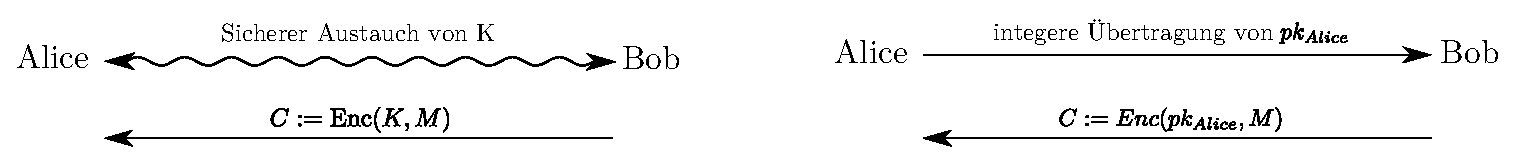
\includegraphics[width=\textwidth]{images/vergleich-symmetrisch-asymmetrisch.eps}
  \caption{Unterschiede in der Vorbereitung von symmetrisch und
    asymmetrisch verschlüsselter Kommunikation}
  \label{fig:asymmenc-symmenc}
\end{figure} Damit Bob eine asymmetrisch verschlüsselte Nachricht an
Alice senden kann, benötigt er ihren öffentlichen Schlüssel. Dieser darf
unverschlüsselt verschickt werden, es muss aber sichergestellt werden,
dass der Schlüssel nicht bei der Kommunikation manipuliert wurde. Dies
geschieht über eine sogenannte \textit{Public Key Infrastructure}, was
hier jedoch nicht weiter vertieft wird.
\section{Sicherheitsbegriffe für asymmetrische Verfahren} Die
Sicherheitsbegriffe, die wir in Kapitel \ref{chap:krypt-begriffe} kennen
gelernt haben, finden mit leicht abgewandelten Definitionen auch bei
asymmetrischen Verfahren Anwendung:

\begin{definition}[Semantische Sicherheit für Public-Key-Verfahren] Ein
  Pub\-lic-""Key-""Ver\-schlüs\-sel\-ungs\-sche\-ma ist \textit{semantisch
    sicher}, wenn es für jede $M$-Verteilung von Nachrichten gleicher Länge,
  jede Funktion $f$ und jeden PPT-Algorithmus $\A$ einen PPT-Algorithmus
  $\B$ gibt, so dass
  \begin{equation*} \Pr\left[\A(1^k, pk, \enc(pk, M)) = f(M)\right] -
    \Pr\left[\B(1^k) = f(M)\right]
  \end{equation*} vernachlässigbar (als Funktion im Sicherheitsparameter)
  ist.
\end{definition}

\begin{definition}[IND-CPA-Sicherheit für
  Public-Key-Verfahren]\indexINDCPA Betrachte folgendes Experiment mit
  einem Herausforderer $\C$ und einem PPT-Angreifer $\A$.
  \begin{itemize}
  \item $\C$ generiert mit dem Generator-Algorithmus ein Schlüsselpaar,
    d.h. er berechnet $(pk, sk)$.
  \item $\A$ erhält $pk$ und kann sich zu jedem Zeitpunkt jedes
    beliebige $\plaint$ mithilfe von $pk$ verschlüsseln.
  \end{itemize}
  \begin{enumerate}
  \item $\A$ wählt zwei Nachrichten $\plaint_1$, $\plaint_2$ gleicher
    Länge.
  \item $\A$ erhält $\ciphert^{*} \coloneqq \enc(pk, \plaint_{b})$ für ein von
    $\C$ zufällig gleichverteilt gewähltes $b \in \{1, 2\}$.
  \item $\A$ gewinnt, wenn er $b$ korrekt errät.
  \end{enumerate} Ein asymmetrisches Verfahren $(\gen, \enc, \dec)$
  heißt IND-CPA-sicher, wenn der Vorteil des Angreifers gegenüber dem
  Raten einer Lösung, also $\Pr \left[ \A \textnormal{ gewinnt} \right] -
  \frac{1}{2}$, für alle PPT-Algorithmen $\A$ vernachlässigbar im
  Sicherheitsparameter $k$ ist.
\end{definition}

Der IND-CPA-Begriff unterscheidet sich also dadurch vom symmetrischen
Fall, dass ein Angreifer $\A$ kein Orakel mehr braucht, sondern
Chiffrate selbst mit dem öffentlichen Schlüssel erzeugen kann.

Auch IND-CCA hat eine Variante für asymmetrische Verfahren, die wir aber
nicht weiter vertiefen.


\section{RSA-Verschlüsselung} Das bekannteste Public-Key-Verfahren ist
RSA\indexRSATextBook (1977). Es ist benannt nach seinen Erfindern
Ronald Rivest, Adi Shamir und Leonard Adleman.

\subsection{Erweiterter Euklidischer Algorithmus}
\label{ssec:eea} Um das Vorgehen der Schlüsselerzeugung des
RSA-Algorithmus erklären zu können, führen wir den \emph{Erweiterten
  Euklidischen Algorithmus} (EEA)\indexEEA als Hilfskonstrukt ein, der es
uns erlaubt, das inverse Element $t$ zu $B$ über einer multiplikativen
Gruppe $\mathbbm{Z}^{\ast}_{A}$ zu bestimmen. Für gegebene Parameter $A$
und $B$ berechnet der EEA neben dem größten gemeinsamen Teiler $\ggT(A,
B)$ zwei ganze Zahlen $s$ und $t$, sodass

\begin{align*} \ggt(A, B) = s \cdot A + t \cdot B\, .
\end{align*}

Für das RSA-Verfahren reicht es, den Spezialfall $\ggT(A,B) = 1$ zu
betrachten, der folgenden Zusammenhang liefert:

\begin{align*} 1 &= s \cdot A + t \cdot B\\ \Leftrightarrow 1 &\equiv t
                                                                \cdot B \pmod A
\end{align*}

Bezüglich $\mathbbm{Z}^*_{A}$ ist $t$ also das zu $B$
multiplikativ-inverse Element. Das Vorgehen betrachten wir beispielhaft
für $B = 23$, zu dem das inverse Element über $\mathbbm{Z}^{\ast}_{192}$
bestimmt werden soll.

Wir betrachten im Folgenden zwei Varianten des erweiterten Euklidischen
Algorithmus.

Der EEA entwickelt zwei Variablen $s$ und $t$ iterativ, sodass gilt:
\begin{align*} s_{i+1} &= s_{i-1} - f_{i+1} \cdot s_{i}\\ t_{i+1} &=
                                                                    t_{i-1} - f_{i+1} \cdot t_{i}
\end{align*} Hierbei ist $f_i = \max \{f : f \cdot B_i \leq A_i\}$
und die größte Zahl, die $R_i > 0$
\begin{beispiel}[EEA] Es sei $A = A_2 = 192 $ und $B = B_2 = 23$. Es
  ist $\ggT(192, 23) = 1$, da B prim und A kein Vielfaches von B ist . Nun
  berechnen wir ausgehend von $i = 2$ in
  \begin{align*} A_i = f_i \cdot B_i + R_i
  \end{align*} jeweils $f_i = \max \{f : f \cdot B_i \leq A_i\}$ und
  $R_i > 0$, bis $R_i = 0$. Dabei ist $A_{i+1} = B_i$ und $B_{i+1} =
  R_i$. Parallel dazu entwickeln wir die Parameter $s$ und $t$ über die
  Gleichungen \emph{vorwärts}. Wir erhalten demnach
  \begin{table}[h] \centering \large
    \begin{tabular}[c]{|c|l|rrr|l|} \hline & Gleichung & $R_i$ & $s_i$ & $t_i$ &\\ 
      \hline 
      \hline 
      (0) & $192 = 1 \cdot 192 + 0 \cdot 23$ & $192$ & $1$ & $0$ &\\
      (1) & $23 = 0 \cdot 192 + 1 \cdot 23$ & $23$ & $0$ & $1$   &\\ 
      \hline 
          & EEA & & & &\\ 
      \hline 
      (2) & $192 = 8 \cdot 23 + 8$ & $8$ & $1$ & $-8$ & $\text{(0)} - 8 \cdot\text{(1)}$\\
      (3) & $23 = 2 \cdot 8 + 7$ & $7$ & $-2$ & $17$ & $\text{(1)} - 2  \cdot \text{(2)}$\\ 
      (4) & $8 = 1 \cdot 7 + 1$ & $1$ & $3$ & $-25$ & $\text{(2)} - 1 \cdot \text{(3)}$\\
      (5) & $7 = 7 \cdot 1 + 0$ & $0$ & $-23$ & $192$ & $\text{(3)} - 7 \cdot\text{(4)}$\\ 
      \hline
    \end{tabular}
  \end{table}
  \subsubsection*{Varianten 1: Vorwärts-Entwicklung} Die vom EEA
  berechneten Werte, das heißt die Parameter $s$ und $t$, stehen in der
  (4). Zeile. Es ist also
  \begin{align*} 1    &= 3 \cdot 192 + (-25) \cdot 23\\ 
    \Leftrightarrow 1 &\equiv (-25) \cdot 23 \pmod{192}\\ 
    \Leftrightarrow 1 &\equiv (192 - 25)\cdot 23 \pmod{192}\\
    \Leftrightarrow 1 &\equiv 167 \cdot 23 \pmod{192}\, \text{,}
  \end{align*} 
  und somit $167$ das zu $23$ multiplikativ-inverse Element bezüglich
  $\mathbbm{Z}^{\ast}_{192}$.
  \subsubsection*{Varianten 2: Rückwärts-Entwicklung} 
  Ebenso ist es möglich, die Parameter $s$ und $t$ \emph{rückwärts} zu
  berechnen. Dazu werden, ausgehend von (2), die Gleichungen (3), (4) und
  (5) aufgestellt und anschließend wie folgt ineinander eingesetzt:
  \begin{align*}
    \begin{split}
      1 &\stackrel{\textit{(4)}}{=} 8 - 1 \cdot 7\\
        &\stackrel{\textit{(3)}}{=} 8 - 1 \cdot (23 - 2 \cdot 8) = -23 + 3 \cdot 8\\ 
        &\stackrel{\textit{(2)}}{=} -23 + 3 \cdot (192 - 8 \cdot 23) = 3\cdot 192 - 25 \cdot 23\\
 [.5cm] &\equiv -25 \cdot 23 \pmod{192}\\
        &\equiv 167 \cdot 23 \pmod{192}
    \end{split}
  \end{align*}
\end{beispiel}

\subsection{Vorgehen}
\label{ch:asymmenc:rsa:vorgehen} Um RSA\indexRSATextBook nutzen zu
können, brauchen wir drei Algorithmen: Einen Generator-Algorithmus
$\operatorname{Gen}$, einen Verschlüsselungsalgorithmus
$\operatorname{Enc}$ und einen Entschlüsselungsalgorithmus
$\operatorname{Dec}$.
\subsubsection{Generator-Algorithmus} Für die Erstellung eines
Schlüsselpaares werden zwei große Primzahlen benötigt. Die Berechnung
des öffentlichen und privaten Schlüssels funktioniert folgendermaßen:
\begin{itemize}
\item Wähle zwei große Primzahlen $P, Q$ mit $P \neq Q$ und
  vorgegebener Bitlänge $k$.
\item Berechne $N = P \cdot Q$.
\item Berechne $\varphi(N) = (P - 1)(Q - 1)$\footnote{$\varphi$
    bezeichnet die Eulersche Phi-Funktion\indexEulerPhiFunction. Sie gibt
    für jede natürliche Zahl n an, wie viele zu n teilerfremde natürliche
    Zahlen es gibt, die nicht größer als n sind: $\varphi(n) \coloneqq \vert
    \{a\in\N \, |\, 1 \le a \le n \land \operatorname{ggT}(a,n) = 1 \}
    \vert$. Insbesondere ist $\varphi(N)$ die Anzahl multiplikativ
    invertierbarer Elemente im Restklassenring $\mathbb{Z}/N\mathbb{Z}$.
    Sie ist multiplikativ, d.h. es gilt für teilerfremde $n$, $m$:
    $\varphi(m\cdot n) = \varphi(m) \cdot \varphi(n)$. Da eine Primzahlen
    $p$ nur durch 1 und sich selbst teilbar ist, gilt $\varphi(p) =
    p-1$. Somit gilt für zwei Primzahlen $p$, $q$ also $\phi(p \cdot q) =
    \phi(p) \cdot \phi(q) = (p-1)(q-1)$.}.
\item Wähle $e \in \{3, \dotsc, \varphi(N) - 1\}$, wobei
  $\ggT(e, \varphi(N)) = 1$.
\item Berechne mit Hilfe des \hyperref[ssec:eea]{EEA} das zu $e$
  multiplikativ-inverse Element $d$ bezüglich $\varphi(N)$, d.h. $d \equiv
  e^{-1} \pmod{\varphi(N)}$.
\end{itemize}

Damit ist der geheime Schlüssel $sk = (N, d)$ und $pk = (N, e)$ der
öffentliche Schlüssel. Üblicherweise werden $P$ und $Q$ zufällig
gleichverteilt aus den ungeraden Zahlen der Bitlänge $k$ gezogen, bis
$P$ und $Q$ prim sind. Der Nachrichtenraum ist \Z{N}.
\subsubsection{Ver- und Entschlüsselung} Für die Ver- und
Entschlüsselungsfunktion gilt:
\begin{align*} \enc(pk, M) & = M^e \mod N \\ \dec(sk, C) & = C^d \mod N
\end{align*}

Wie immer muss $\dec(\enc(M)) = M$ gelten. Für die Korrektheit von RSA
bedeutet das, dass
\begin{align*} (M^e)^d \equiv M^{ed} \equiv M \pmod N
\end{align*} erfüllt sein muss. Um das zu beweisen, verwenden wir den
Kleinen Satz von Fermat und den Chinesischen Restsatz.
\begin{theorem}[Kleiner Satz von Fermat]\indexFermatLittleTheorem Für
  primes $P$ und $M \in \{1, \dotsc, P-1\}$ gilt: $M^{P-1} \equiv 1 \mod
  P$.
\end{theorem}
\begin{beweis} ohne Beweis
\end{beweis} Daraus folgt auch: $\forall M \in \Z P, \alpha \in
\mathbbm{Z} : (M^{P-1})^{\alpha} \cdot M \equiv M \mod P$.

\begin{theorem}[Chinesischer Restsatz]\indexChineseRemainderTheorem Sei
  $N = P \cdot Q$ mit $P, Q$ teilerfremd. Dann ist die Abbildung $\mu : \Z
  N \rightarrow \Z P \times \Z Q$ mit $\mu(M) \equiv (M \mod P, M \mod Q)$
  bijektiv.
\end{theorem}
\begin{beweis} ohne Beweis
\end{beweis} Daraus folgt auch: $(X \equiv Y \mod P) \land (X \equiv Y
\mod Q) \Rightarrow X \equiv Y \mod N$.

\begin{theorem}[Korrektheit von RSA] Sei $N = P \cdot Q$ mit $P, Q$
  teilerfremd und prim. Seien weiter $e, d$ teilerfremd wie oben. Dann ist
  $M^{ed} \equiv M \mod N$ für alle $M \in \Z N$.
\end{theorem}

\begin{beweis} Nach Definition gilt $e \cdot d \equiv 1 \mod
  (P-1)(Q-1)$. Daraus folgt:
  \begin{align*}
    (P-1)(Q-1) \mid ed - 1 \quad & \Rightarrow \quad P-1 \mid ed - 1\\
                                 & \Rightarrow \quad ed = \alpha (P-1) + 1 \quad (\text{für }\alpha \in \mathbbm{Z})\\ 
                                 & \Rightarrow \quad M^{ed} = (M^{(P-1)})^{\alpha} \cdot M \stackrel{\text{Fermat}}\equiv M \mod P
  \end{align*} 
  Analog ist $M^{ed} \equiv M \mod Q$. Da $N = P \cdot Q$
  ergibt sich mithilfe des Chinesischen
  Restsatzes\indexChineseRemainderTheorem:
  \[
    (M^{ed} \equiv M \mod P) \land (M^{ed} \equiv M \mod Q) \Rightarrow M^{ed} \equiv M \mod N
  \] \qed
\end{beweis}

Das bisher behandelte Verfahren wird häufig \textit{Textbook-RSA}
\indexRSATextBook genannt und umfasst das grundlegende Prinzip von
RSA. Textbook-RSA weist einige Schwächen auf, die im nächsten Abschnitt
genauer besprochen werden. Deshalb sollte es in der Praxis nicht
verwendet werden.

\subsection{Sicherheit von (Textbook-)RSA}
\label{ch:asymmenc:rsa:sicherheit} Bevor wir die Sicherheit von RSA
betrachten, benötigen wir einen Sicherheitsbegriff, an dem wir uns bei
der Beurteilung von asymmetrischen Verschlüsselungsverfahren orientieren
können. Wir definieren semantische Sicherheit, vergleichbar mit der
Definition für symmetrische Chiffren in Kapitel
\ref{ch:sicherheitsbegriffe:semantischesicherheit} und äquivalent zu
IND-CPA.

RSA ist deterministisch, d.h. eine Nachricht $M$ wird unter Verwendung
desselben Schlüssels $pk$ immer zum gleichen Chiffrat $C_M$
verschlüsselt. Dadurch kann ein PPT-Angreifer zwei Chiffrate
(z.B. $\enc(pk, \text{annehmen})$ und $\enc(pk, \text{ablehnen})$)
effizient voneinander unterscheiden. RSA ist also nicht IND-CPA-sicher
(und damit auch nicht semantisch sicher).

Ein mathematisches Problem, dass eng mit der Sicherheit von RSA
verknüpft ist, ist die Faktorisierung von natürlichen Zahlen. Hierbei
geht es darum eine gegebene Zahl $N$ in seine Primzahlfaktoren zu
zerlegen. Zur Zeit ist kein Algorithmus bekannt, der das
Faktorisierungsproblem in Polynomialzeit löst. Wäre ein solcher
Algorithmus bekannt, so könnte man leicht RSA \glqq brechen\grqq , indem
man $N$ in $P$ und $Q$ faktorisiert und dann mit Hilfe des euklidischen
Algorithmus und dem öffentlichen Schlüssel den geheimen Schlüssel
berechnet. Umgekehrt ist jedoch nicht bekannt, ob ein Algorithmus der
RSA bricht \footnote{Im Sinne von schwächeren
  Sicherheitsbegriffen. Unter gewissen mathematischen Annahmen (die nicht
  mit der Faktorisierung zu verwechseln sind) kann man beispielsweise
  zeigen, dass es schwierig ist, aus ei- nem gegebenen RSA-Chiffrat den
  kompletten Klartext zu berechnen. Diese Sicherheitsbegriffe werden in
  dieser Vorlesung aber nicht weiter thematisiert.} auch einen Algorithmus
impliziert, der das Faktorisierungsproblem effizient löst. Dies ist eine
wichtige offene Forschungsfrage der Kryptographie. \footnote{In der
  gängigen populärwissenschaftlichen Literatur und Magazinen liest man
  häufig Sätze wie \glqq RSA zu brechen ist so schwierig wie
  Faktorisieren\grqq. Dies ist, wie oben argumentiert, mit Vorsicht zu
  genießen.}

Textbook-RSA hat noch einige andere Angriffspunkte, die im Folgenden
umrissen werden.

\begin{description}
\item[Wahl von $e$:] Aus Effizienzgründen liegt es auf den ersten Blick
  nahe, den Parameter $e$ aus dem öffentlichen Schlüssel nicht für jeden
  Benutzer neu zu berechnen, sondern für alle gleich zu wählen. Da diese
  Wahl nur den öffentlichen Schlüssel betrifft, scheint diese
  Einschränkung nicht kritisch zu sein, führt jedoch zu Problemen, wenn
  dieselbe Nachricht $M$ an mehrere unterschiedliche Benutzer
  verschlüsselt gesendet wird.
  
  Sei beispielsweise $e=3$. Ein PPT-Angreifer, der die drei öffentlichen
  Schlüssel $pk_1, pk_2, pk_3$ kennt, mit denen $M$ verschlüsselt wurde,
  kann sich die Nachricht $M$ berechnen. Hierzu verwendet man den
  chinesischen Restsatz:

  Es gibt ein $X$ mit
  \begin{align*} X \equiv M^3 \mod N_1\\ X \equiv M^3 \mod N_2\\ X
    \equiv M^3 \mod N_3\\
  \end{align*} und mit dem chinesischen Restsatz
  \begin{align*} X \equiv M^3 \mod N_1N_2N_3
  \end{align*}

  Da $M < N_1, N_2, N_3$, gilt insbesondere $M^3<N_1N_2N_3$, womit die
  dritte Wurzel von $X$ in $\mathbbm{Z}$ gezogen und damit $M$ berechnet
  werden kann.
  
\item[Wahl von $N$:] Nutzen zwei Benutzer Schlüssel mit dem selben $N$,
  ergeben sich zwei weitere Angriffe:
  \begin{itemize}
  \item Wird wieder dieselbe Nachricht $M$ mit zwei öffentlichen
    Schlüsseln $(N, e_1)$ und $(N, e_2)$ chiffriert und gilt weiterhin
    $\text{ggT}(e_1, e_2) = 1$ in $\Z{}$, kann ein PPT-Angreifer aus den
    Chiffraten $M$ berechnen:
    \begin{alignat*}{2} re_1 + se_2 & = 1\\ \Longrightarrow C_1^rC_2^s
      \mod N &= M^{re_1}M^{se_2} &\mod N\\ &= M^{re_1 + se_2} &\mod N\\ &= M
      &\mod N
    \end{alignat*}
  \item Ist $N$ für zwei Benutzer $A$, $B$ gleich, dann kennen beide
    Benutzer $P$ und $Q$, also auch $\varphi(N)$. Damit kann $A$ mit $pk_A =
    (N, e_A)$ nun einfach ein $d_B'$ zu Benutzer $B$ mit $pk_B = (N, e_B)$
    berechnen mit
    \[d_B'=e_B^{-1} \mod \varphi(N).\] Dies geht genauso wie die
    RSA-Schlüsselerzeugung.
  \end{itemize}
\item[Homomorphie:]\indexRSAHomomorphie Auf der multiplikativen Gruppe
  $(\mathbbm{Z}, \cdot)$ des RSA-Modulus gilt der Zusammenhang
  \begin{alignat*}{2} \enc(pk, M_1) \cdot \enc(pk, M_2) &\equiv M_1^e
    \cdot M_2^e & \pmod N \\ &\equiv (M_1 \cdot M_2)^e & \pmod N\\ &\equiv
    \enc(pk, M_1 \cdot M_2) & \pmod N
  \end{alignat*} und wir sehen, dass RSA homomorph ist.  Folgendes
  Beispiel soll veranschaulichen, zu welchen Zwecken die Homomorphie
  ausgenutzt werden kann:
  \begin{beispiel} Wir betrachten eine Auktion mit dem Auktionsleiter
    $A$ und zwei Bietern $B_1$ und $B_2$. Damit keiner der Interessenten
    einen anderen knapp überbietet oder sich von den Geboten anderer in
    seiner eigenen Abgabe beeinflussen lässt, nimmt der Auktionator die
    Gebote verschlüsselt entgegen. Dafür hat er seinen öffentlichen
    Schlüssel $pk_A$ zur Verfügung gestellt. Das Gebot eines Bieters wird
    chiffriert und zur Aufbewahrung an den Auktionator geschickt. Wenn die
    Zeit abgelaufen ist, werden keine neuen Preisvorschläge mehr angenommen,
    die eingegangenen Gebote entschlüsselt und der Höchstbietende ermittelt.
    
    Der unehrliche Bieter $B_2$ kann nun seinen Preisvorschlag
    mithilfe des verschlüsselten Gebots von $B_1$ zu seinen Gunsten
    wählen. Dafür setzt er z.B. $C_2 = C_1 \cdot \enc({pk_A, 2})$ oder, wenn
    er besonders sparsam ist, $C_2 = C_1 \cdot \enc({pk_A, 1001/1000 \mod
      N})$. Damit kann er das Gebot von $B_1$ verdoppeln bzw. knapp
    überbieten, ohne dass der Auktionator und der ehrliche Bieter $B_1$ ihm
    Betrug nachweisen können.
  \end{beispiel}
\end{description}

\subsection{Sicheres RSA}\label{ssec:sicheres-rsa} Wir haben
festgestellt, dass RSA deterministisch und damit nicht semantisch sicher
ist. Die gepaddete Variante \emph{RSA optimal asymmetric encryption
  padding} (RSA-OAEP)\indexRSAOAEP dagegen ist IND-CCA-sicher im
\emph{Random Oracle Model}\indexRandomOracleModel\footnote{Im Random
  Orcale Model geht man von einer idealisierten Form von Hashfunktionen
  aus, die in der Realität nicht existiert. Trotzdem wurde bisher kein in
  diesem Modell als sicher bewiesenes Verfahren \glqq gebrochen\grqq. Die
  Bewertung des Random Orcale Models ist ein viel diskutiertes Thema,
  worauf hier aber nicht weiter eingegangen werden soll.}. Wir verwenden
dabei eine Zufallszahl $R$, mit deren Hilfe wir die Nachricht $M$ vor
dem Verschlüsseln abwandeln. Zu diesem Zweck wird die in Abbildung
\ref{fig:rsa-oaep} dargestellte Konstruktion von Hashfunktionen $G, H$
verwendet. $R$ muss nach dem Entschlüsseln nicht gespeichert werden, da
es sich mit $Y \oplus H(X)$ berechnen lässt, aber $\enc_R(M)$ lässt sich
nun nicht mehr so einfach mit anderen Chiffraten abgleichen.

\begin{figure}[h]
  \begin{center} \unitlength=1mm \linethickness{0.4pt} \hspace{-3 cm}
    \begin{picture}(60,60)
      
      \put(0,50){\framebox(30,5){$m$}}
      \put(32,50){\framebox(15,5){$000$}} \put(55,50){\framebox(20,5){$R$}}
      
      \put(15,45){\line(0,1){5}} \put(39,45){\line(0,1){5}}
      \put(15,45){\line(1,0){24}} \put(25,45){\vector(0,-1){40}}
      
      \put(65,50){\vector(0,-1){45}}
      
      \put(45,35){\circle{7}} \put(45,34){\makebox(0,0)[cb]{$G$}}
      \put(25,35){\circle{4}} \put(23,35){\line(1,0){18.5}}
      \put(65,35){\vector(-1,0){16.5}}
      
      \put(45,20){\circle{7}} \put(45,19){\makebox(0,0)[cb]{$H$}}
      \put(65,20){\circle{4}} \put(25,20){\vector(1,0){16.5}}
      \put(48.5,20){\line(1,0){18.5}}
      
      \put(0,0){\framebox(45,5){$X$}} \put(55,0){\framebox(20,5){$Y$}}
      
    \end{picture}
  \end{center}
  \caption{Pad-Funktion von RSA-OAEP ($G,H$ sind Hashfunktionen)}
  \label{fig:rsa-oaep}
\end{figure}

\subsubsection{Verschlüsselung mit RSA-OAEP} Um mit RSA-OAEP zu
verschlüsseln, wendet man erst das Padding-Verfahren aus Grafik
\ref{fig:rsa-oaep} an und verschlüsselt danach mit RSA, wobei das
Schlüsselpaar wie bei RSA generiert wurde:
\begin{itemize}
\item Wähle $R$ zufällig.
\item Berechne
  \begin{align*} X & = m \oplus G(R) \\ Y & = R \oplus H(X).
  \end{align*}
\item Verschlüssele gemäß:
  \[ \enc_{OAEP}(pk, M) = (X||Y)^e \mod N.
  \]
\end{itemize}
\subsubsection{Entschlüsselung mit RSA-OAEP} Zur Entschlüsselung eines
Chiffrats $C$ wird erst RSA-Entschlüsselung angewendet, danach wird das
Padding rückgängig gemacht:
\begin{itemize}
\item Rekonsturiere $(X||Y) = \dec(sk, C)$.
\item rekonstruiere $R$ mit $R = Y \oplus H(X)$.
\item Berechne $M$ mit $M = X \oplus G(R)$.
\end{itemize}

\subsection{Bedeutung von RSA}\indexRSATextBook\indexRSAOAEP Im
Gegensatz zu den meisten symmetrischen Chiffren basiert RSA als Beispiel
einer asymmetrischen Verschlüsselungstechnik nicht auf einfachen,
bit-orientierten sondern auf einer mathematischen Funktion. Der für Ver-
und Entschlüsselung, sowie für die Schlüsselerzeugung nötige
Rechenaufwand steigt dadurch ungemein: Ein naiver
Exponentiationsalgorithmus benötigt für die Berechnung einer modulo
$l$-Bit-Zahl $\omega(l)$ Bitoperationen.

Nichtsdestotrotz wird RSA in der Praxis häufig eingesetzt. Es macht sich
relativ einfache Arithmetik zunutze und die Ähnlichkeit zwischen Ver-
und Entschlüsselungsfunktion vereinfachen die Implementierung
zusätzlich. Mit einfachen Anpassungen ($e = 3$ bei Verschlüsselung,
Chinesischer Restsatz nutzen bei Entschlüsselung) kann RSA so weit
beschleunigt werden, dass es die Laufzeit betreffend gegenüber anderen
Verschlüsselungsverfahren konkurrenzfähiger wird.

\section{ElGamal-Verschlüsselung}
\label{ch:asymenc:elgamal} Das ElGamal-Verfahren\indexElGamal (1985)
macht sich die Schwierigkeit zunutze, das DLOG-Problem\indexDLOGProblem,
also die Berechnung von diskreten Logarithmen in zyklischen Gruppen, zu
lösen. Unter einer zyklischen Gruppe versteht man eine Gruppe
$\mathbbm{G}$, bei der ein sogenanntes Erzeugerelement $g$ existiert, so
dass $\mathbbm{G} = \langle g \rangle \coloneqq \{g^k \mid k \in
\mathbbm{Z}\}$.

\subsection{Vorgehen} Für die Schlüsselerzeugung wird eine ausreichend
große Gruppe $\mathbbm{G}$ mit Primordnung $p$ mit dem Erzeuger $g$
verwendet.
\subsubsection{Schlüsselerzeugung} Zur Schlüsselerzeugung wird ein $x
\in {2,\dots, p-1}$ zufällig gewählt und $h \equiv g^x$ berechnet. Dann
sind
\begin{align*} 
  pk &= (\mathbbm{G}, g, h)\\ sk &= (\mathbbm{G}, g, x)
\end{align*}

\subsubsection{Ver- und Entschlüsselung} Ver- und Entschlüsselung sind
definiert durch
\begin{align*} 
&\enc(pk, M) = (g^y, h^y M) \\ 
&\dec(sk, (g^y, C)) = \frac{C}{(g^y)^x},
\end{align*} 
wobei $y$ bei jeder Verschlüsselung neu zufällig aus $\{2, \dots, p-1\}$
gewählt wird. Es gilt also 
\begin{align*} 
C &\equiv h^y M \\ 
\Leftrightarrow \quad M& \equiv \frac{C}{h^y} \equiv \frac{C}{g^{xy}}
                         \equiv \frac{C}{(g^y)^x} 
\end{align*}

\subsubsection{Homomorphie}\indexElGamalHomomorphie Wie RSA ist auch
ElGamal homomorph:
\begin{align*} 
\enc({pk,M}) \cdot \enc({pk,M'}) &= (g^y, g^{xy} \cdot M)\cdot (g^{y'},
                                   g^{xy'} \cdot M')\\ 
                                 &= (g^{y+y'}, g^{x(y + y')}\cdot M  \cdot M')\\ 
                                 &= \enc({pk, M \cdot M'})
\end{align*}

\subsubsection{Sicherheit des Verfahrens und Wahl geeigneter Gruppen}
Für die Sicherheit des ElGamal-Verfahrens ist die Wahl eine geeigneten
Gruppe $\mathbb{G}$ von entscheidender Bedeutung. ElGamal ist genau dann
IND-CPA-sicher, wenn in $\mathbb{G}$ die \emph{decisional
  Diffie-Hellman}-Annahme\indexDecisionalDiffieHellman (DDH-Annahme)
gilt.
\begin{definition}[DDH-Annahme]\label{def:ddh} In einer zyklischen
  Gruppe $\mathbbm{G} = \langle g \rangle$ sind die Tupel $(g^a, g^b,
  g^{ab})$ und $(g^a, g^b, g^c)$ für zufällig und unabhängig gewählte
  $a,~b,~c$ von jedem PPT-Angreifer nur mit im Sicherheitsparameter $k$
  vernachlässigbarer Wahrscheinlichkeit unterscheidbar.
\end{definition}

Damit die DDH-Annahme gilt, muss $\mathbbm{G}$ ausreichend viele
Elemente haben. Ansonsten könnte die DDH-Annahme schon durch
ausprobieren aller Elemente gebrochen werden. Geeignete Kandidaten für
$\mathbbm{G}$ sind echte Untergruppen von $\mathbbm{Z}^*_p$ mit $p$ prim
und $|\mathbbm{G}| \approx 2^{2048}$. Effizienter sind Untergruppen von
elliptischen Kurven $\boldsymbol{\mathsf{E}}(\mathbbm{F}^*_q)$ mit einer
Gruppengröße von $|\mathbbm{G}| \approx 2^{200}$.

\subsection{Erweiterung des Urbildraums} Ein Problem des klassischen
ElGamal-Verfahrens ist, dass nur Nachrichten $M \in \mathbbm{G}$
verschlüsselt werden können. In der Praxis sind jedoch die meisten
Nachrichten außerhalb der gewählten Gruppe, weshalb die Korrektheit der
notwendigen Operationen nicht garantiert werden kann. Es existieren
jedoch verschiedene Ansätze, dieses Problem zu lösen und den Raum
möglicher Nachrichten flexibler zu gestalten.

\subsubsection{Nachrichtenumwandlung} Die Nachrichtenumwandlung
\indexMessageTransformation erlaubt es, beliebige Nachrichten fester
Länge zu verschlüsseln, ohne den eigentlichen Algorithmus anpassen zu
müssen. Die Länge der möglichen Nachrichten wird dabei durch die Größe
der zugrunde liegenden Gruppe festgelegt.

\paragraph*{Verfahren} Im Folgenden werde $M$ zunächst als Bit-String
aufgefasst. Wir wählen $p > 2 $ prim und setzen $\mathbbm{G} \subset
\mathbbm{Z}^*_p$ als Untergruppe der Quadrate\footnote{Die Untergruppe
  der Quadrate von $\mathbbm{Z}^*_p$ besteht aus den Elementen $\{x^2
  \text{ mod } p\ \vert\ x \in \mathbbm{Z}^*_p\}$. Falls $p > 2$ prim ist,
  besteht diese Untergruppe aus $\frac{p - 1}{2}$ Elementen. Jedes
  Element, mit Ausnahme der Eins, kann als Gruppenerzeuger dienen.} von
$\mathbbm{Z}^*_p$, wobei $\mathbbm{G}$ die Ordnung $q = \frac{(p -
  1)}{2}$ hat.  Es sei $n$ die Länge des Bit-Strings der Gruppenordnung
$q$. Dann können wir die Nachricht $M \in \{0, 1\}^{n - 1}$ beliebig
wählen und interpretieren sie im weiteren Verlauf als ganze Zahl
äquivalent zu ihrer Binärdarstellung. Da $M$ auch die Null darstellen
kann und die Null in multiplikativen Gruppen nicht vorhanden ist, setzen
wir $\tilde{M} = M + 1$. Folglich ist $ 1 \leq \tilde{M} \leq q$ und
daher $\tilde{M} \in \mathbbm{Z}^*_p$. Nach der Eigenschaft einer
quadratischen Untergruppe ist somit $\hat{M} = \tilde{M}^2 \text{ mod }
p \in \mathbbm{G}$.

Damit kann $\hat{M}$ analog zum obigen Verfahren verschlüsselt
werden. Zum Entschlüsseln berechnet der Empfänger aus $\hat{M}$ als
Zwischenschritt $\tilde{M} = \sqrt{\hat{M}}\ \text{mod}\ p\ \in [1, q]$
und erhält mit $M = \tilde{M} - 1$ die ursprüngliche Nachricht $M$ in
der Binärdarstellung. $\hat{M}$ ist durch normales Entschlüsseln mit
ElGamal zu berechnen.

Ein Nachteil dieses Verfahrens ist, dass die Nachrichtenumwandlung, je
nach gewählter Gruppe, nicht effizient möglich ist.

\subsubsection{Hash-ElGamal} Eine weitere Variante, die Einschränkung
der Nachrichten auf Elemente der gewählten Gruppe aufzuheben, ist das
Hash-ElGamal-Kryptosystem\indexHashElGamal. Es realisiert ein Verfahren,
dass zu allen Nachrichten $M \in \{0, 1\}^l$ mit Hilfe der bereits
bekannten Bausteine und einer Hashfunktion ein Chiffrat der gleichen
Länge bestimmt. Im Gegensatz zur Nachrichtenumwandlung bilden wir $M$
dabei nicht auf die Gruppe ab. Die Sicherheit des Kryptosystems beruht
ausschließlich auf der Annahme, dass der diskrete Logarithmus nicht
effizient berechnet werden kann und ist, zumindest falls
rechtseindeutig, nicht von der Wahl der Hashfunktion abhängig. Das
Hash-ElGamal-Verfahren bietet somit Sicherheit auf gleichem Niveau, ist
in der Verwendung, aufgrund des größeren Urbildraums, jedoch deutlich
flexibler.

\paragraph*{Verfahren} Es seien die Gruppe $\mathbbm{G} \subset
\mathbbm{Z}^*_p$ und das Schlüsselpaar $(pk,sk)$ analog zu ElGamal
gewählt und berechnet. Sei zudem $H \colon \mathbbm{G} \rightarrow
\{0,1\}^l$ eine beliebige Hashfunktion, die in Bitfolgen der Länge $l$
abbildet.

Wähle, um eine Nachricht $M \in \{0,1\}^l$ zu verschlüsseln, $y
\leftarrow \mathbbm{Z}_p$ zufällig gleichverteilt, berechne $Y = g^y\
\text{mod}\ p$ und sende das Tupel
\begin{align*} (Y, H(h^y) \oplus M) = (Y, C)
\end{align*}

Unter Zuhilfenahme des privaten Schlüssels $sk = (\mathbbm{G}, g, x)$
kann der Ursprungstext $M$ aus dem Chiffrat-Tupel zurückgerechnet
werden:
\begin{align*} M = H(Y^x) \oplus C
\end{align*}

\section{Fazit} Asymmetrische Verschlüsselung\indexEncryptionAsymm
bietet einige Vorteile, die es bei symmetrischer Verschlüsselung nicht
gibt. Insbesondere wird für jeden Teilnehmer nur ein Schlüsselpaar
benötigt, damit alle Teilnehmer verschlüsselt kommunizieren können,
während bei symmetrischen Verfahren die Anzahl an Schlüsseln quadratisch
in der Anzahl der Teilnehmer wächst.

Wie symmetrische Verfahren auch, aber im Gegensatz zu
informationstheoretisch sicheren Verfahren, bauen asymmetrische
Verschlüsselungsverfahren auf Probleme, von denen man annimmt, dass sie
schwer zu lösen sind. Bei RSA ist dies das Ziehen von $e$-ten Wurzeln
modulo $N$, bei ElGamal die DDH-Annahme.

Alle bekannten asymmetrischen Verschlüsselungsverfahren haben einen
deutlich höheren Rechenaufwand als symmetrische Verfahren
\indexEncryptionSymm, da sie nicht auf Elementaroperationen, wie das
Shiften von Bits oder einem XOR beruhen, sondern auf komplexen
mathematischen Operationen in algebraischen Strukturen. Deshalb
verwendet man in der Praxis oft sogenannte \emph{hybride}
Verschlüsselungsverfahren\indexEncryptionHybrid. Ein Beispiel hierfür
ist \emph{TLS}\indexTLS, das in \hyperref[cha:keyexchange]{Kapitel 8}
näher besprochen wird.
\chapter{Symmetrische Authentifikation von Nachrichten}
\label{cha6}

Bisher haben wir uns nur mit der Frage beschäftigt, wie ein Kommunikationsteilnehmer Bob eine Nachricht an Alice für einen unbefugten Lauscher unverständlich machen, also verschlüsseln kann. Wir haben uns noch nicht der Frage nach der Authentifikation einer Nachricht gewidmet. 
Der Angreifer könnte mit dem entsprechenden Zugriff auf den Übertragungskanal sogar eine verschlüsselte Kommunikation beeinflussen, deren Inhalt er nicht versteht. Er kann Nachrichten abfangen, verändern und wieder auf den Weg bringen, ohne dass Alice oder Bob etwas von dem Zwischenstopp der Nachricht bemerken.
Falls ein Angreifer trotz der Verschlüsselungsmaßnahmen außerdem in der Lage ist, die Kommunikation zu verstehen, könnte er sogar \textit{gezielt} den Inhalt von Nachrichten verändern.
Es kann jedoch auch ohne Angreifer geschehen, dass der Kommunikationskanal gestört und Bobs Nachricht durch technische Einwirkungen abgewandelt wird.

Im besten Fall erhält Alice dann eine unbrauchbare Nachricht und kann bei Bob eine Wiederholung anfordern. Im schlechtesten Fall ist die Veränderung zufällig (oder vom Angreifer gewollt) sinnvoll und beeinflusst damit das weitere Vorgehen der beiden Kommunikationsteilnehmer.

%TODO: Erklärung von Integrität zum ersten Aufkommen hinzufügen und hier entfernen
\section{Ziel}
Angesichts dessen, dass wir uns unseren Kommunikationskanal nicht immer aussuchen können, hätten wir gern einen Mechanismus, der uns ermöglicht, eine erhaltene
Nachricht auf Fehler und Veränderungen zu überprüfen (Integrität) und den Absender zu bestimmen (Authentizität). Dafür erstellt Bob für seine Nachricht $M$
zusätzlich eine "`Unterschrift"' $\sigma$ und überträgt diese gemeinsam mit $M$. Alice erhält das Paar $(M,\sigma)$ und überprüft, ob die Unterschrift auf die
erhaltene Nachricht passt.

Um ein funktionierendes und gegen einen Angreifer möglichst sicheres Unterschriftensystem zu erhalten, müssen einige Anforderungen erfüllt sein:
\begin{itemize}
  \item Bob muss $\sigma$ aus der bzw. für die Nachricht $M$ berechnen können
  \item Alice muss $\sigma$ zusammen mit $M$ verifizieren können
  \item ein Angreifer soll kein gültiges $\sigma$ für ein selbst gewähltes $M$ berechnen können
\end{itemize} 

\section{MACs}
\label{ch:symauth:macs}
Die Idee von \textit{Message Authentication Codes} (MACs) basiert auf der Grundannahme, dass Alice und Bob bereits ein gemeinsames Geheimnis $K$ besitzen. Es
ist also ein symmetrisches Verfahren. Signatur und Verifikation der Unterschrift funktionieren dann wie folgt:
\begin{itemize}
  \item \textbf{Signieren:} $\sigma \leftarrow \sig(K,M)$
  \item \textbf{Verifizieren:} $\ver(K,M,\sigma) \in \{0,1\}$
\end{itemize}
Es muss immer gelten: $\ver(K,M, \sig(K,M)) = 1$. Eine mit $\sig$ erstellte Signatur muss also unter demselben Schlüssel $K$ von $\ver$ als gültig ausgezeichnet
werden.

\section{Der EUF-CMA-Sicherheitsbegriff}
\label{ch:symauth:sicherheit}
Damit ein MAC uns nicht nur vor Übertragungsfehlern sondern auch vor einem Angreifer schützt, verlangen wir, dass kein Angreifer selbstständig ein
Nachrichten-Signatur-Paar finden kann, das gültig ist.

Er bekommt dafür ein Signaturorakel mit vor ihm verborgenem Schlüssel $K$, mit dem er Nachrichten seiner Wahl signieren kann. Er
gewinnt, wenn er die Signatur einer Nachricht $M$ korrekt vorhersagen kann, ohne $M$ vorher an das Orakel gegeben zu haben. Etwas strukturierter sieht der
Angriff für einen PPT-Angreifer $\mathcal{A}$ so aus:
\begin{enumerate}
  \item $\mathcal{A}$ erhält Zugriff auf ein Signaturorakel $\sig(K,\cdot)$
  \item $\mathcal{A}$ wählt ein Nachrichten-Signatur-Paar $(M^*,\sigma^*)$
  \item $\mathcal{A}$ gewinnt, wenn das Orakel zu $M^*$ $\sigma^*$ ausgibt, wenn also $\ver(K,M^*,\sigma^*) = 1$, und das Signaturorakel vorher $M^*$ noch
  nicht von $\mathcal{A}$ erhalten hat
\end{enumerate}
Dieses Schema bildet passive Angriffe ab, bei denen der Angreifer keinen Zugriff auf die $\ver$-Funktion hat, sondern "`blind"' signiert. Wenn es für ein $M$
nur ein einziges, gültiges $\sigma$ gibt, ist dieser Angriff dagegen äquivalent zu einer Attacke mit Zugriff auf die $\ver$-Routine. 

Einen Signaturalgorithmus, der sicherstellt, dass $\mathcal{A}$ dieses Spiel nur vernachlässigbar oft gewinnt, nennen wir \textit{EUF-CMA-sicher} (EUF:
Existential Unforgeability, CMA: Chosen Message Attack).

\section{Konstruktionen}

\subsection{Hash-then-Sign Paradigma}
Eine Signatur, die so lang ist, wie das ursprüngliche Dokument, erfüllt zwar ihren Zweck, was Datenintegrität und Authentizität angeht, ist jedoch
unpraktikabel. Wir suchen also einen Mechanismus, der uns bei variabler Nachrichtenlänge eine kurze Signatur einer Nachricht $M$ ermöglicht. Dafür bieten sich
sofort Hashfunktionen an.

Die Idee des \emph{Hash-then-Sign} Paradigmas ist also, nicht die vollständige Nachricht $M~\in~\{0,1\}^*$ zu signieren, sondern den aus dieser Nachricht berechneten
Hashwert $H(M) \in \{0,1\}^k$. Die Sicherheit des MACs ist dabei sowohl von der verwendeten Hashfunktion als auch vom Signaturalgorithmus
abhängig.~\\

\begin{theorem}
Sei $(\sig, \ver)$ EUF-CMA-sicher und $H$ eine kollisionsresistente Hashfunktion. Dann ist der durch 
\begin{align*}
\sig(K,M) &= \sig(K,H(M))\\
\ver(K,M,\sigma) &= \ver(K,H(M),\sigma) 
\end{align*}
erklärte MAC EUF-CMA-sicher.~\\
\end{theorem}

\begin{beweis}[Entwurf]
\label{ch:symauth:eufcma-beweis}
Der EUF-CMA-Angreifer $\mathcal{A}$ muss entweder eine Kollision in der Hashfunktion $H$ finden und kann damit auf dieselbe Signatur von zwei Nachrichten
schließen oder er muss einen einzelnen Hashwert $H(M)$ finden, für den er eine Signatur errechnen kann.
\end{beweis}

\subsection{Pseudorandomisierte Funktionen}\label{ssec:prf}
Wenn man sich die Berechnung eines MACs als eine einfache Funktion im mathematischen Sinne vorstellt und damit die Errechnung eines "`frischen"' MACs zum
Finden eines unbekannten Funktionswertes wird, erkennt man schnell, dass Regelmäßigkeit in einer solchen Funktion zu Sicherheitslücken führt. Zielführender ist
es, die Funktionswerte möglichst zufällig auf ihre Urbilder zu verteilen.
\begin{definition}[Pseudorandomisierte Funktion (PRF)]
Sei\\ 
$\text{\textit{PRF}}\colon\{0,1\}^k \times \{0, 1\}^k \rightarrow \{0,1\}^k$
eine über $k \in \mathbbm{N}$ parametrisierte Funktion. $PRF$ heißt Pseudorandom Function (PRF), falls für jeden PPT-Algorithmus $\mathcal{A}$ die Funktion
\begin{equation*}
\text{Adv}_{\text{\textit{PRF}},\mathcal{A}}^{prf}(k) := \Pr \lbrack \mathcal{A}^{\text{\textit{PRF}}(K,\cdot)}(1^k) = 1 \rbrack - \Pr \lbrack \mathcal{A}^{R(\cdot)}(1^k) = 1 \rbrack
\end{equation*}
vernachlässigbar ist, wobei $R: \{0,1\}^k \rightarrow \{0,1\}^k$ eine echt zufällige Funktion ist.~\\
\end{definition}

Ein Kandidat für eine solche PRF ist eine Hash-Konstruktion: $PRF(K,X) = H(K,X)$. Allerdings lässt sich eine solche Konstruktion manchmal, wie bereits in
Abschnitt \ref{ch:hash:merkledamgard} bei Merkle-Damgård ausgenutzt, nach der Berechnung von $H(K,X)$ auch ohne Zugriff auf das Geheimnis $K$ noch auf
$H(K,X,X')$ erweitern. Das führt dazu, dass die PRF-Eigenschaft für Eingaben unterschiedlicher Länge nicht mehr hält. Abbildung \ref{fig:symauth:prf} verdeutlicht das.

\begin{figure}[h]
\begin{center}
\unitlength=1mm
\linethickness{0.4pt}
\hspace{-3 cm}
\begin{picture}(70,40)

\put(10,27){\vector(1,0){15}}
\put(17,28){\makebox(0,0)[cb]{IV}}

\put(30,37){\vector(0,-1){7.5}}
\put(33,31){\makebox(0,0)[cb]{$K$}}

\put(25,24.5){\framebox(10,5){$F$}}

\put(35,27){\vector(1,0){12}}
\put(52,37){\vector(0,-1){7.5}}
\put(55,31){\makebox(0,0)[cb]{$X$}}

\put(47,24.5){\framebox(10,5){$F$}}

\put(57,27){\vector(1,0){8}}
\put(75,25){\makebox(0,0)[cb]{$H(K,X)$}}


\put(0,10){\vector(1,0){15}}
\put(7,11){\makebox(0,0)[cb]{IV}}

\put(20,20){\vector(0,-1){7.5}}
\put(23,15){\makebox(0,0)[cb]{$K$}}

\put(15,7.5){\framebox(10,5){$F$}}

\put(25,10){\vector(1,0){12}}
\put(42,20){\vector(0,-1){7.5}}
\put(45,15){\makebox(0,0)[cb]{$X$}}

\put(37,7.5){\framebox(10,5){$F$}}

\put(47,10){\vector(1,0){12}}
\put(64,20){\vector(0,-1){7.5}}
\put(67,15){\makebox(0,0)[cb]{$X'$}}

\put(59,7.5){\framebox(10,5){$F$}}

\put(69,10){\vector(1,0){8}}
\put(89,8){\makebox(0,0)[cb]{$H(K,X,X')$}}

\put(53,4){\makebox(0,0)[cb]{\Large{$\Uparrow$}}}
\put(53,-2){\makebox(0,0)[cb]{$H(K,X)$ bekannt}}

\end{picture}
\end{center}
\caption{\emph{Merkle-Damgård}-Konstruktion $H_{MD}$. Es ist möglich, an einen bereits bekannten Hashwert $H(K,X)$ einen Wert $X'$ anzuhängen und trotzdem
einen korrekten Hashwert zu erzeugen.}
\label{fig:symauth:prf}
\end{figure}

\begin{theorem}
Sei $\text{PRF}\colon\{0,1\}^k \times \{0,1\}^k \rightarrow \{0,1\}^k$ eine PRF und $H \colon \{0,1\}^* \rightarrow \{0,1\}^k$ eine kollisionsresistente
Hashfunktion.
Dann ist der durch $\sig(K,M) = \text{\textit{PRF}}(K,H(M))$ gegebene MAC EUF-CMA-sicher.
\end{theorem}
\vspace{10pt}

\begin{beweis}[Entwurf]
Sei $\mathcal{A}$ ein erfolgreicher EUF-CMA-Angreifer auf ein durch $\sig(K,M) = \text{\textit{PRF}}(K,H(M))$ gegebenen MAC. Dann können wir annehmen,
dass $\mathcal{A}$ eine Fälschung $(M^*,\sigma^*)$ mit einer noch nicht signierten Nachricht $M^*$ berechnen kann. Wir können also $\mathcal{A}$ als
\textit{PRF}-Unterscheider auffassen, der mit nicht-vernachlässigbarer Wahrscheinlichkeit $\text{\textit{PRF}}(K,H(M^*))$ vorhersagt. Eine Vorhersage ist jedoch
nur dann möglich, wenn \textit{PRF} keinen Zufall ausgibt. Da \textit{PRF} jedoch nach Definition nur mit vernachlässigbarer Wahrscheinlichkeit von echtem
Zufall unterscheidbar ist, kann es einen solchen \textit{PRF}-Unterscheider nicht geben.
\end{beweis}

\subsection{HMAC}
Im Abschnitt zu \hyperref[ssec:prf]{pseudorandomisierten Funktionen} haben wir gesehen, dass Signaturverfahren, die Merkle-Dåmgard nutzen,
dem EUF-CMA-Sicherheitsbegriff im Allgemeinen nicht genügen. Ein Angreifer, dem $\sigma = H(K,M)$ bekannt ist, erhält durch Anfügen eines Blockes $X$ problemlos den korrekten Hashwert $H(K,M,X)$ und somit die Signatur der Nachricht $M,X$.
Dennoch ist es möglich, EUF-CMA-sichere MACs zu konstruieren, die mittels einer Merkle-Dåmgard-Konstruktion signieren.
Eines der verbreitetsten Verfahren ist der \textit{Keyed-Hash Message Authentication Code}, der HMAC. Das Signieren einer Nachricht
funktioniert dabei wie folgt:
\begin{equation*}
\sig(K,M) = H(K \oplus \textit{opad}, H(K \oplus \textit{ipad}, M))
\end{equation*}
Dabei sind \textit{opad}, das \textit{outer padding}, und \textit{ipad}, das \textit{inner padding}, zwei Konstanten der Blocklänge $m$ der Hashfunktion, die bei jedem Signaturvorgang gleich bleiben. Üblich\footnote{Sowohl im RFC 2104, sowie in einer Veröffentlichung des NIST und in diverser Fachliteratur werden diese Werte (als Standard) vorgeschlagen. Siehe: ~\\~\\ \url{http://tools.ietf.org/html/rfc2104} \\ \url{http://csrc.nist.gov/publications/fips/fips198-1/FIPS-198-1_final.pdf}} ist es, $opad = \{0x5C\}^{m/8}$ und $ipad = \{0x36\}^{m/8}$ zu wählen. Das Verifizieren funktioniert analog zu der in \ref{ch:symauth:macs} gegebenen Definition.

Immun gegen den in Abbildung \ref{fig:symauth:prf} vorgestellten Angriff ist HMAC aufgrund seiner verschachtelten Struktur. Die Nachricht
$M$, die es zu Signieren gilt, wird in jeweils zwei Hash\-vorgängen verarbeitet. Für eine Nachricht $M,X$ ist 
\begin{equation*}
H(K \oplus \textit{opad}, H(K \oplus \textit{ipad}, M), X)
\end{equation*} 
aber offensichtlich keine gültige Signatur. Der Angreifer müsste einen Nachrichtenblock $X$ bereits im inneren Hashvorgang unterbringen. Da er dafür allerdings $H$ invertieren, oder das Geheimnis $K$ kennen müsste, schlägt der Angriff fehl. 

Selbstverständlich muss, obwohl HMAC das eben angesprochene Problem löst, keine Merkle-Dåmgard-Funktion verwendet werden. Für jede pseudorandomisierte Hashfunktion genügt HMAC dem EUF-CMA-Sicherheitsbegriff.
\chapter{Asymmetrische Authentifikation von Nachrichten}
\label{cha:asymmauth}

Wie wir bereits bei den Verschlüsselungsverfahren festgestellt haben, weisen symmetrische Verfahren einige Unbequemlichkeiten auf. Allen voran stellt sich das Problem der Schlüsselverteilung, wenn für die Kommunikation zwischen zwei Partnern bei beiden derselbe Schlüssel vorhanden sein muss. Dieses Problem stellt sich natürlich umso mehr, wenn wir über einen nicht vertrauenswürdigen Kanal kommunizieren. Selbst für die Authentifikation unserer Nachrichten, die wir im Zweifelsfall nur betreiben, weil wir dem Kanal nicht vertrauen, müssen wir unter einigem Aufwand Schlüssel mit unseren Kommunikationspartnern festlegen.

Weiterhin ermöglicht symmetrische Authentifikation in keiner sinnvollen Weise, dass wir von uns veröffentlichte Dokumente oder Nachrichten unterschreiben und damit die Urheberschaft für jeden nachprüfbar machen können. Zur Authentifikation des Dokuments sollte schließlich jeder befähigt sein, der sich dafür interessiert. Wenn wir mit symmetrischen Verfahren arbeiten, bedeutet das, dass wir zur Prüfung den Schlüssel herausgeben müssen, mit dem wir das Dokument signiert haben. Das bedeutet aber auch, dass jeder Interessierte nun nicht nur zur Prüfung der bereits bestehenden Signatur in der Lage ist, sondern auch eigene Signaturen erstellen kann. Damit ist die Urheberschaft einer Unterschrift nicht mehr gesichert.

Es bietet sich ein Verfahren an, bei dem die Prüfung einer Signatur nicht mit einem privaten Schlüssel erfolgt. Dieses System kennen wir bereits aus dem Kapitel \ref{ch:asymmenc}. Bei der Verwendung von asymmetrischen Verfahren zur Authentifikation verwenden wir die folgenden Algorithmen:
\begin{itemize}
  \item \textbf{Schlüsselgenerierung:} $(pk, sk) \leftarrow \keygen(1^k)$
    \begin{itemize}
      \item $pk$ : öffentlicher Schlüssel
      \item $sk$ : privater Schlüssel
      \item $k$ : Sicherheitsparameter
    \end{itemize}
  \item \textbf{Signieren:} $\sigma \leftarrow \sig(sk,M)$
  \item \textbf{Verifizieren:} $\ver(pk,M,\sigma) \in \{ 0,1 \}$
\end{itemize}
$\sig$ und $\ver$ müssen korrekt sein, d.h. es muss wie bei MACs gelten:
\begin{equation*}
    \forall (pk,sk) \leftarrow \keygen(1^k), \forall M, \forall \sigma \leftarrow \sig(sk,M) : \ver(pk,M,\sigma) = 1
\end{equation*}
Wir passen außerdem die Definition der EUF-CMA-Sicherheit aus Abschnitt
\ref{ch:symauth:sicherheit} an asymmetrische Verfahren an.

\begin{definition}
Sei \A~ ein PPT-Algorithmus.
\begin{enumerate}
\item \A~erhält Zugriff auf ein Signarorakel $\sig(sk, \cdot)$ sowie den
  entsprechenden öffentlichen Schlüssel $pk$.
\item \A~darf nun polynomiell viele Nachrichten $\plaint_i$ an das
  Orakel schicken und erhält $\sigma_i$ mit $\ver(\pkey, \plaint_i, \sigma_i)=1$ als Antwort.
\item \A~gibt als (potentielle) Fälschung ein Nachrichten-Signatur-Paar
  $(\plaint^*,\sigma^*)$ aus.
\item \A~gewinnt, wenn $\sigma^*$ eine gültige Signatur für
  $\plaint^*$ ist, d.h. $\ver(\pkey, \plaint^*, \sigma^* = 1)$, und $\plaint^*
  \neq \plaint_i$ für alle $i$ ist, d.h. $\plaint^*$ nicht zu den
  Nachrichten gehört, die sich \A~vom Orakel hat signieren lassen.
\end{enumerate} 

Ein asymmetrisches Signaturverfahren ist EUF-CMA-sicher, wenn jeder
beliebige PPT-Angreifer \A~ das oben genannte Spiel nur mit im
Sicherheitsparameter $k$ vernachlässigbarer Wahrscheinlichkeit gewinnt. 
\end{definition}

Die Definition unterscheidet sich also dadurch vom symmetrischen Fall,
dass \A~kein Verifikationsorakel braucht, sondern Signaturen selbst mit
dem öffentlichen Schlüssel prüfen kann.

\section{RSA}
Wir betrachten zuerst RSA als Kandidaten für ein asymmetrisches Signaturverfahren. RSA besteht, wie in Kapitel \ref{ch:asymmenc:rsa:vorgehen} entwickelt,
aus den folgenden Algorithmen:
\begin{alignat*}{2}
& \enc(\pkey, \plaint) &= \plaint^e & \mod N\\
& \dec(\skey, \ciphert) &= \ciphert^d  & \mod N
\end{alignat*}
Unser privater Schlüssel ist $\skey = (N, d)$ und der öffentliche
Schlüssel ist $\pkey = (N, e)$. RSA hat die nützliche Eigenschaft, dass
sich daraus sehr intuitiv ein Signaturverfahren ableiten
lässt\footnote{Oft liest man, dass das Signieren von Nachrichten immer dem
  Verschlüsseln mit dem geheimen Schlüssel entspricht. Dies gilt jedoch
  im Allgemeinen nicht. RSA ist hier eine seltene Ausnahme!}:
\begin{alignat*}{3}
& \sig(\skey, \plaint) & = \plaint^d & \mod N\\
& \ver(\pkey, \plaint, \sigma) & = 1 : \Leftrightarrow \plaint = \sigma^e & \mod N 
\end{alignat*}
Zur Schlüsselgenerierung nutzen wir den Algorithmus aus
\ref{ch:asymmenc:rsa:vorgehen}.

Das Verfahren hat jedoch einige Nachteile:
\begin{description}
    \item[Signatur \glqq unsinniger\grqq~Nachrichten:] Ein Angreifer
      wählt zunächst ein beliebiges $\sigma \in \mathbbm{Z}$. Dann kann
      er mithilfe des öffentlichen Schlüssels $\pkey$ zu dieser Signatur
      einfach ein $\plaint$ generieren, zu dem die Signatur $\sigma$
      passt: $\plaint := \sigma^e \mod N$.\\ 
    Zwar ist für diesen Angriff im ersten Moment keine sinnvolle Nutzung
    ersichtlich, da der Angreifer keine Kontrolle darüber hat, für
    welche Nachricht er eine Signatur fälscht, die Problematik eines
    Missbrauchs besteht jedoch prinzipiell. Dieser Angriff bricht also
    die für ein Signaturverfahren geforderte EUF-CMA-Sicherheit.
  \item[Homomorphie von RSA:] Angenommen, ein Angreifer ist im Besitz
    zweier Signaturen $\sigma_1$, $\sigma_2$ zu den Nachrichten
    $\plaint_1$, $\plaint_2$. Dann kann er eine gültige Signatur
    $\sigma_3$ für
    eine Nachricht $\plaint_3 = \plaint_1 \cdot \plaint_2 \mod N$
    berechnen mit
    \begin{alignat}{2}
      \sigma_3 &= \plaint_3^d  & \mod N\\
               &=  (\plaint_1 \cdot \plaint_2)^d & \mod N \\
               &= \plaint_1^d \cdot \plaint_2^d &\mod N\\
               &= \sigma_1 \cdot \sigma_2 &\mod N\\ 
    \end{alignat}
  \end{description}
  Aus der Homomorphie kann man sich einen Angreifer bauen, der das
  EUF-CMA-Sicherheitsexperiment gewinnt: 
  \begin{beispiel}
    Sei \A~ein PPT-Algorithmus und \C~ein Challenger im
    EUF-CMA-Sicherheitsexperiment. Das Experiment läuft wie folgt ab.
    \begin{itemize}
    \item \A~wählt zwei Nachrichten $M_1$ und $M_2$ und sendet diese an
      \C
    \item \C~erstellt die Signaturen $\sigma_1$, $sigma_2$ und sendet
      diese an \A
    \item \A~ berechnet $M_3=M_1M_2 \mod N$ und
      $\sigma_3=\sigma_1\sigma_2 \mod N$ und gibt diese aus.
    \end{itemize}
    Damit hat \A~eine Gültige Signatur gefälscht und gewinnt das Experiment.
  \end{beispiel}
Wie bereits bei der RSA-Verschlüsselung in Kapitel \ref{ch:asymmenc:rsa:sicherheit} können wir diese Probleme lösen, indem wir die Nachricht vor der Verarbeitung padden:
\begin{align*}
\sig(\skey,\plaint) &= (\text{pad}(\plaint))^d \mod N\\
\ver(\pkey,\sigma,\plaint) &= 1 :\Leftrightarrow \sigma^e \mod N \text{ ist gültiges Padding für } \plaint
\end{align*}
Das so entstandene Signaturverfahren nennt sich (RSA-)PSS (\emph{Probabilistic Signature Scheme}) und ist wie RSA-OAEP (als Teil der \emph{PKCS}) kryptographischer Standard.\footnote{\url{http://www.emc.com/emc-plus/rsa-labs/standards-initiatives/pkcs-rsa-cryptography-standard.htm}}
%TODO: Zeichnungen zum Erstellen und Prüfen einer Signatur

Unter Verwendung idealer Hashfunktionen und mit der Annahme, dass die
RSA-Funktion schwierig zu invertieren ist, ist RSA-PSS heuristisch
EUF-CMA sicher\footnote{D.h. sicher im Random-Oracle-Modell}. Ein Angreifer ist gezwungen, die RSA-Funktion direkt anzugreifen. Der beste bekannte Angriff basiert auf der Faktorisierung von $N$ (unter Verwendung des Zahlkörpersiebs). Die Parameter werden ähnlich wie bei RSA-OAEP gewählt und haben so eine Länge von meistens 2048 Bit. Um eine effiziente Verifikation der Signaturen zu gewährleisten, ist es außerdem ohne Schwierigkeiten möglich, den Parameter $e$ klein zu wählen.


\section{ElGamal}
Analog zum ElGamal-Verschlüsselungssystem aus Kapitel
\ref{ch:asymenc:elgamal} betrachten wir nun ein Signaturverfahren über
zyklischen Gruppen.
\subsection{erste Idee}
Sei für unseren ersten Versuch der geheime Schlüssel $\skey = (\G, g,
x)$ und der öffentliche Schlüssel $\pkey = (\G, g, g^x)$. Dann bietet
sich die Verwendung von ElGamal zur Erzeugung einer Signatur auf diese
Art an: 
\begin{align*}
\sig(\skey,M) &= a \text{ mit } a \cdot x = M \mod \left|\G\right|\\
\ver(\pkey,\sigma,M) &= 1 :\Leftrightarrow (g^x)^a = g^M
\end{align*}
Allerdings lässt sich diese Konstruktion auf einfache Art brechen, indem
mit $x = M a^{-^1} \mod \G$ der geheime Schlüssel berechnet wird. 
Der Ansatz, \textit{\glqq Signieren ist Verschlüsseln mit dem geheimen
  Schlüssel\grqq}, den wir bei RSA verwendet haben, führt hier also
nicht zu einem sicheren Signaturverfahren.
\subsection{Schlüssel- und Signaturerzeugung}
Für die Schlüssel gilt weiterhin $\skey = (\G, g,
x)$, $\pkey = (\G, g, g^x)$. 
Für sie Signaturerzeugung wählt Alice, die eine Nachricht signieren will, eine
zufällige, in $\Z{n}$ invertierbare Zahl $e \in \{1, \dots, q - 1\}$,
wobei $q=|\G|$ und berechnet damit:
\begin{align*}
a &:= g^e \in |G|\\
b &:= (M - a \cdot x) \cdot e^{-1} \mod q
\end{align*}
$a$ ist Gruppenelement, $b$ ist eine Zahl in $\Z{q}$. 
Damit gilt $a \cdot x + e \cdot b = M$. Das Signaturverfahren ist nun
$\sig(\skey,M) = (a, b)$.

Für das Verifikationsverfahren werden nun zwei Gruppenelemente $v_1,
v_2 \in \G$ berechnet mit
\begin{align*}
  v_1 &= (g^x)^a \cdot a^b\\
  v_2 &= g^M.
\end{align*}
Das Verifikationsverfahren ist nun
\begin{align*}
\ver(\pkey,\sigma,M) = 1 : & \Leftrightarrow v_1 = v_2 \\
 &\Leftrightarrow (g^x)^a \cdot a^b = g^M \\
 &\Leftrightarrow  g^{ax} \cdot g^{be} = g^M
\end{align*}
Doch auch bei dieser Variante gibt es noch einige offene Angriffspunkte:
\begin{description}
	\item[Doppelte Verwendung von $e$:]
	Wird der zufällige Parameter $e$ mehrmals zur Erzeugung von Signaturen verwendet, kann der geheime Schlüssel $x$ aus den beiden Signaturen errechnet werden. Seien die Signaturen $(a = g^e, b, M)$ und $(a' = g^{e'} = a, b', M')$. Dann ergibt sich durch Aufaddieren und Umformen
	der Gleichungen
	\begin{align*}
	&a \cdot x + e \cdot b = M\\
	\land \quad &a \cdot x + e \cdot b' = M'\\
	\Rightarrow \quad &e = \frac{M - M'}{b - b'}
	\end{align*}
	Mit bekanntem $e$ kann wiederum auf den geheimen Schlüssel $x$
        geschlossen werden.\footnote{Im Signaturverfahren der
          Spielekonsole \textit{PlayStation 3} (PS 3) wurde dem
          Zufallsparameter $e$ ein immer gleicher Wert zugewiesen,
          wodurch der geheime Schlüssel berechnet werden konnte. Dadurch
          wurde es möglich, unautorisierte Anwendungen, wie
          \textit{gecrackte} Spiele, auf der PS 3 auszuführen. Die
          Erklärung zu diesem erfolgreichen Angriff ist
          \href{https://www.youtube.com/watch?v=4loZGYqaZ7I}{hier} zu
          finden, wobei der Angriff auf das Signaturverfahren ab Minute
          35:30 beschrieben wird.} Bei zufälliger Wahl geschieht es nur
        vernachlässigbar oft, dass zwei Mal dasselbe $e$ ausgewählt wird
        und infolgedessen ausgenutzt werden kann .
	\item[Erzeugung "`unsinniger"' Signaturen:]
	Durch günstige Wahl der Parameter ist es möglich, auch ohne Kenntnis des Schlüssels $x$ gültige Signaturen zu erzeugen. Wähle zunächst $c$
	zufällig. Setze außerdem:
	\begin{align*}
	a &:= g^cg^x = g^{c+x}\\
	b &:= -a
	\end{align*}
        Dies implieziert $e=c+x$. 
	Dann ist $(a, b)$ eine gültige Signatur zu $M$ mit
	\begin{align*}
          M &= -ac\\
            &= a \cdot x - a \cdot (c + x)\\
            &= a \cdot x + b \cdot e,\\
	\end{align*}
        denn es gilt 
        \begin{alignat*}{3}
          &&                 & (g^x)^a\cdot a^b       &= &g^M\\
          && \Leftrightarrow & g^{ax} \cdot a^{-a}     &= &g^{-ac}\\
          && \Leftrightarrow & g^{ax} \cdot (g^e)^{-a} &= &g^{-ac}\\
          && \Leftrightarrow & g^{ax-a(c+x)}            &= &g^{-ac}\\
          && \Leftrightarrow & g^{-ac}                 &= &g^{-ac}
        \end{alignat*}
      \end{description}
      \subsection{Beispiel}
      Im Folgenden werden Schlüsselerzeugung, Signieren und Verifizieren beispielhaft
      in der multiplikative Gruppe $\G = \Z{17}^{*}$ mit Ordnung $16$ gezeigt. 
      \subsubsection*{Schlüsselerzeugung}
      Es sind $\skey = (\G, g, x)$ und $\pkey = (\G, g, g^x)$. Als
      Erzeuger wird $g=3$, als Zufallszahl wird $x=11$
      gewählt. Es sind also $\skey = (\G, 3, 11)$ und $\pkey = (\G, 3,
      3^{11})\equiv (\G, 3, 7)$.
      \subsubsection*{Signieren}
      Alice will eine Nachricht $\plaint = 10$ mit $sk$ signieren. Dazu
      wählt sie einen zufälligen, in $\Z{16}$ invertierbaren  Exponenten
      $e= 13$ und $e^{-1}=5$. Dann ist $\sigma = 
      (a, b)$ mit 
      \begin{align*}
       a &:= g^e\\
         &= 3^{13} \equiv 12 \\
       b &:= (\plaint-a  \cdot x) \cdot e^{-1} & \mod |\G|\\
          &= (10 - 11 \cdot 12) \cdot 7^{-1} & \mod |\G|\\
          &\equiv (10 - 11*12) \cdot 5 \equiv 14 & \mod |\G|
      \end{align*}
      \subsubsection*{Verifizieren}
      Es ist
      \begin{align*}
        v_1 & = (g^x)^a \cdot a^b\\
            & = 7^{12} \cdot 12^{14} \\
            & \equiv 13 \cdot 15\\
            & \equiv 8 \mod 17\\
        v_2 & = g^M \\
            &= 3^{10} \\
            &\equiv 8 \mod 17,\\
      \end{align*}
      also gilt $v_1=v_2$ und die Signatur ist gültig.
     

      \section{Hash-Then-Sign-Paradigma}
      Analog zum symmetrischen Fall wollen wir mithilfe eines
      Hash-Then-Sign-Paradigmas Nachrichten beliebiger Länge signieren können.
      \begin{theorem}[Hash-Then-Sign-Paradigma]
        Sei $(\keygen, \sig, \ver)$ EUF-CMA-sicher und $H$ eine
        kollisionsresistente Hashfunktion. Dann ist das durch  
        \begin{align*}
          \keygen'(1^k) &= \keygen(1^k)\\
          \sig'(\skey,M) &= \sig(\skey,H(M))\\
          \ver'(\pkey,M,\sigma) &= \ver(\pkey,H(M),\sigma)
        \end{align*}
        definierte Signaturverfahren EUF-CMA-sicher.~\\
      \end{theorem}

      Der Beweis dieses Theorems verläuft analog zu \ref{ch:symauth:eufcma-beweis}.

      Die Verwendung einer kollisionsresistenten Hashfunktion ermöglicht
      eine Abwehr gegen die Erzeugung "`unsinniger"' Signaturen, denn
      die errechneten "`unsinnigen"' Klartexte müssen nun zusätzlich
      denselben Hashwert erzeugen wie die Originalnachricht. 


\section{Digital Signature Algorithm (DSA)}
Aus der Anwendung des Hash-Then-Sign-Paradigmas auf das ElGamal-Signaturverfahren entsteht unter Verwendung einer kollisionsresistenten
Hashfunktion $H$ der \emph{Digital Signature Algorithm} (DSA):
\begin{align*}
a &:= g^e\\
b &:= (H(M) - a \cdot x) \cdot e^{-1} \mod \left|\G\right|
\end{align*}
mit der Signatur $\sigma = (a,b)$.

Der DSA ist nach RSA der zweitwichtigste Signaturalgorithmus und wurde 1994 standardisiert.\footnote{Der aktuelle Standard findet sich auf \url{http://csrc.nist.gov/groups/ST/toolkit/digital_signatures.html}} Für die Bewertung von DSA wirkt sich nachteilig aus, dass für jede neue Signatur eine frische Zufallszahl gewählt werden muss (ein guter Zufallsgenerator wird also
vorausgesetzt) und dass die Verifikation einer DSA-Signatur im Vergleich zu einer RSA-Signatur mit kleinem Modulus deutlich langsamer ist.

Ob DSA EUF-CMA-sicher ist, steht noch nicht eindeutig fest.

\chapter{Schlüsselaustauschprotokolle}
\label{cha:keyexchange}

In diesem Kapitel widmen wir uns der offenen Frage nach dem
Schlüsselaustauschproblem, das insbesondere bei der Besprechung von
symmetrischen Verschlüsselungs- und Signaturverfahren einige Male
aufgekommen ist. Zwei Kommunikationspartner Alice und Bob können ohne
vorherigen Schlüsselaustausch keine sichere Verbindung
einrichten. Allerdings werden sie nicht jedes Mal die Möglichkeit haben,
sich vor ihrer eigentlichen Kommunikation privat zu treffen, um einen
gemeinsamen Sitzungsschlüssel auszuhandeln. Vielleicht kennen sie
einander nicht einmal persönlich, auf jeden Fall aber wäre ein solches
Vorgehen sichtlich nicht praktikabel.

Alice und Bob müssen also die unsichere Leitung zum Schlüsselaustausch
verwenden. Den Schlüssel im Klartext darüber zu senden, würde einen
Mithörer trivial in die Situation bringen, auch den verschlüsselten Teil
der darauf folgenden Kommunikation mitzulesen. Der neue
Sitzungsschlüssel $\key$ von Alice und Bob muss also bereits so über die
Leitung gesendet werden, dass ein Lauscher nicht in der Lage ist, den
Schlüssel zu rekonstruieren. Dabei sind folgende grundlegende Szenarien
denkbar:\indexSecretKeyInfrastructure\indexPublicKeyInfrastructure
\begin{itemize}
  \item Alice und Bob besitzen bereits einen alten Schlüssel $\key'$ aus
    einem früheren Austausch und möchten ein frisches $\key$ erzeugen
  \item es existierte eine Secret-Key-Infrastruktur mit einer
    Schlüsselzentrale (Alice besitzt einen Schlüssel $\key_A$, Bob $\key_B$
    und die Schlüsselzentrale beide)
  \item es existiert eine Public-Key-Infrastruktur ($\pkey_A, \pkey_B$
    sind öffentlich, Alice besitzt $\skey_A$, Bob besitzt $\skey_B$)
  \item Alice und Bob besitzen ein gemeinsames Passwort
  \item Alice und Bob besitzen keine gemeinsamen Informationen
\end{itemize}


\section{Symmetrische Verfahren}
Als Grundszenario für symmetrische Verfahren wird hier ein System mit
einer Secret-Key-Infrastruktur\indexSecretKeyInfrastructure
gewählt. Das bedeutet, dass jeder Teilnehmer einen geheimen,
symmetrischen Schlüssel mit der Schlüsselzentrale hat. Jeder
Verbindungsaufbau mit einem anderen Teilnehmer beginnt deshalb mit einer
Anfrage an die Zentrale. Da die Zentrale die Anlaufstelle für viele
Teilnehmer ist, sollte die Kommunikation mit dieser Stelle möglichst
minimiert werden, was die vollständige Kommunikation der beiden
Teilnehmer Alice und Bob über die Zentrale ausschließt. Gleichzeitig
sind jedoch die Leitungen nicht vertrauenswürdig, sodass die
Kommunikation über große Strecken verschlüsselt stattfinden sollte.

\subsection{Kerberos}
Eine Lösung für dieses Szenario bietet das Protokoll \emph{Kerberos}
\indexKerberos an, das in Abbildung \ref{fig:keyex:kerberos} in seiner
ursprünglichen Form dargestellt ist. Alice sendet dabei der
Schlüsselzentrale eine Anfrage, die ihren Namen und den ihres
gewünschten Gesprächspartners erhält und bekommt dafür von der Zentrale
zwei Pakete zurück, von denen eines mit ihrem und eins mit Bobs
Schlüssel verschlüsselt ist. Beide Pakete erhalten den gemeinsamen
Sitzungsschlüssel $K$, sowie die Lebensdauer $L$ des Schlüssels und
einen Zeitstempel $T_{KC}$ der Schlüsselzentrale, der Replay-Attacken
erschwert.  Alice entpackt das an sie adressierte Paket, erhält den
Sitzungsschlüssel und leitet nach Prüfung von $L$ und $T$ das für Bob
vorbereitete Paket weiter. Sie fügt außerdem eine mit $K$ verschlüsselte
Nachricht bei, in der sie ihre Identität und einen von ihr erstellten
Zeitstempel $T_A$ einfügt.

Bob überprüft seinerseits den Zeitstempel der Zentrale und die
Lebensdauer des Sitzungsschlüssels und dechiffriert dann Alices
Nachricht mit dem neuen Sitzungsschlüssel. Er kann nun sowohl den
Zeitstempel überprüfen als auch, ob die Anfrage an die Schlüsselzentrale
vom selben Teilnehmer stammt wie die mit dem Sitzungsschlüssel
chiffrierte Nachricht. Außerdem kann er bei erfolgreicher
Entschlüsselung sicher sein, dass Alice $K$ besitzt. Er sendet nun
seinerseits eine mit $K$ verschlüsselte Nachricht an Alice, mit der er
nachweist, dass er den Sitzungsschlüssel besitzt. Mit der Erhöhung des
Zeitstempels kann er außerdem beweisen, dass er die korrekte Nachricht
erhalten und dechiffriert hat.

\begin{figure}[h]
\begin{center}
\unitlength=1mm
\linethickness{0.4pt}
\hspace{-3 cm}
	\begin{picture}(120,60)(-10,0)
		\put(0,53){\makebox(0,0)[cb]{\texttt{Alice}$_{\key_A}$}}
		\put(100,53){\makebox(0,0)[cb]{\texttt{Schlüsselzentrale (KC)$_{\key_A, \key_B}$}}}
		\put(120,28){\makebox(0,0)[cb]{\texttt{Bob$_{\key_B}$}}}
	
		\put(0,2){\line(0,1){50}}
		\put(100,30){\line(0,1){22}}
		\put(120,2){\line(0,1){25}}
		
		\put(50,46){\makebox(0,0)[cb]{(Alice, Bob)}}
		\put(0,45){\vector(1,0){100}}
	
		\put(50,36){\makebox(0,0)[cb]{$\enc(\key_A,(T_{KC}, L, \key, \text{Bob}))$, $\enc(\key_B, (T_{KC}, L, \key, \text{Alice}))$}}
		\put(100,35){\vector(-1,0){100}}
		
		\put(60,20){\makebox(0,0)[cb]{$\enc(\key, (\text{Alice}, T_A))$, $\enc(\key_B, (T_{KC}, L, \key, \text{Alice}))$}}
		\put(0,19){\vector(1,0){120}}
		
		\put(60,10){\makebox(0,0)[cb]{$\enc(K, T_A+1)$}}
		\put(120,9){\vector(-1,0){120}}
	
	\end{picture}
\end{center}
\caption{Ursprüngliches Schlüsselaustauschprotokoll Kerberos. $T_X$ bezeichnet einen von $X$ ausgestellten Zeitstempel, $\key$ den
erzeugten Sitzungsschlüssel für Alice und Bob und $L$ seine Lebensdauer.}
\label{fig:keyex:kerberos}
\end{figure}

Die verschachtelte Konstruktion von Kerberos verhindert
Man-in-the-Middle-Angriffe. Die Kodierung der Absender- und
Empfängernamen durch die Schlüsselzentrale ermöglicht eine
Authentifizierung der Kommunikationsteilnehmer und der Einsatz von
Zeitstempeln sowie die Zuordnung einer Lebensdauer zu einem Schlüssel
erschwert zudem Replay-Attacken.  Nichtsdestotrotz ist für das Protokoll
ein aktiv sicheres Verschlüsselungsverfahren nötig. Die Sicherheit von
Kerberos ist nicht formal geklärt.

\section{Asymmetrische Verfahren}
Als Grundlage für die folgenden Schlüsselaustauschprotokolle nutzen wir
eine Public-Key Infrastruktur. Die Schlüssel werden wie in Kapitel
\ref{ch:asymmenc} von den Teilnehmern selbst erzeugt. Jeder hält also
seinen privaten Schlüssel geheim. Die öffentlichen Schlüssel
hinterliegen an einem allgemein zugänglichen Ort und sind von einer
vertrauenswürdigen Stelle zertifiziert.

\subsection{Public-Key Transport} Das einfachste Verfahren, das sich zum
Schlüsselaustausch in Public-Key-Infrastruktur
\indexPublicKeyInfrastructure anbietet, nennt sich \emph{Public-Key
Transport}\indexPublicKeyTransport. Alice erzeugt einen
Sitzungsschlüssel, den sie für die Kommunikation mit Bob verwenden
will. Die bereits bestehende Infrastruktur wird nun dafür genutzt, den
Sitzungsschlüssel mit Bobs öffentlichem Schlüssel zu chiffrieren und an
Bob zu senden (siehe Abb.
\ref{fig:keyex:publickeytransport}).

\begin{figure}[h]
\begin{center}
\unitlength=1mm
\linethickness{0.4pt}
\hspace{-3 cm}
\begin{picture}(30,10)
\put(0,2){\makebox(0,0)[cb]{$\text{Alice}_{\skey_A}$}}
\put(10,3){\vector(1,0){40}}
\put(30,4){\makebox(0,0)[cb]{$C \coloneqq \enc(\pkey_B, \key)$}}
\put(55,0.5){\makebox(10,5){$\text{Bob}_{\skey_B}$}}
\end{picture}
\end{center}
\caption{Während des Protokolls Public-Key Transport wählt Alice einen Sitzungsschlüssel $\key$ und sendet ihn unter Ausnutzung der zur
Verfügung stehenden Public-Key-Infrastruktur an Bob.}
\label{fig:keyex:publickeytransport}
\end{figure}

Vorausgesetzt, das verwendete Public-Key-Verfahren ist IND-CPA-sicher,
kann der Angreifer $\ciphert$ nicht von Zufall unterscheiden oder den
darin enthaltenen Sitzungsschlüssel extrahieren. Public-Key Transport
ermöglicht also passive Sicherheit gegenüber einem Angreifer, der
$\ciphert$ auf der Leitung mithören kann.

Allerdings bietet das Verfahren in dieser Form keine Möglichkeit zur
Authentifizierung der Kommunikationsteilnehmer an. Das lässt sich durch
das Hinzufügen von Signaturen wie in Abbildung
\ref{fig:keyex:publickeytransportauth} lösen. Trotzdem ist es dann noch
immer möglich, einen Replay-Angriff durchzuführen und $\ciphert$ zu
einem späteren Zeitpunkt noch einmal zu senden, ohne dass Bob der Fehler
sofort auffällt.

\begin{figure}[h]
\begin{center}
\unitlength=1mm
\linethickness{0.4pt}
\hspace{-3 cm}
\begin{picture}(120,10)(-15,0)
\put(0,0){\makebox(0,0)[cb]{$\text{Alice}_{\skey_{\text{PKE,}A}, \skey_{\sig, A}}$}}
\put(16,3){\vector(1,0){80}}
\put(55,4){\makebox(0,0)[cb]{$(C \coloneqq \enc(\pkey_{\text{PKE,}B}, \key),$}}
\put(55,-2){\makebox(0,0)[cb]{$\sigma \coloneqq \sig(\skey_{\sig, A}, C))$}}
\put(110,0){\makebox(10,5){$\text{Bob}_{\skey_{\text{PKE,}B}, \skey_{\sig, B}}$}}
\end{picture}
\end{center}
\caption{Digitale Signaturen ermöglichen den Ausbau des Protokolls Public-Key Transport auf die Authentifikation der Teilnehmer.}
\label{fig:keyex:publickeytransportauth}
\end{figure}


\subsection{Diffie-Hellman-Schlüsselaustausch} 
\label{sec:ddh-key-exchange}\indexDiffieHellmanKeyExchange,
Historisch gesehen entstand das uns schon bekannte
ElGamal-Verschlüsselungsverfahren (1985) aus dem
Diffie-Hellman-Schlüsselaustausch (1976)
den wir im folgenden betrachten werden. Auch hier benötigen wir eine
ausreichend große, zyklische Gruppe $\G = \langle g \rangle$ mit Ordnung
$q$. Alice und Bob wählen sich jeweils eine Zufallszahl $x, y \in
\mathbbm{Z}_q$ und schicken $g^x$ bzw. $g^y$ an den jeweils
anderen. Jeder von beiden ist nun in der Lage, $g^{xy}$ zu
berechnen. Abbildung \ref{fig:keyex:dh} erläutert dies.

Das Berechnen des gemeinsamen Geheimnisses $g^{xy}$ als Außenstehender
bezeichnet man als \emph{computational Diffie-Hellman}-Problem
(CDH-Problem)\indexComputationalDiffieHellmanProblem.  Dabei hat ein
Angreifer Zugriff auf das Erzeugerelement und die beiden Zahlen
$g^{x}$, $g^{y}$. Die Sicherheit des Verfahrens beruht auf der
sogenannten \emph{computational Diffie-Hellman}-Annahme
(CDH-Annahme)\indexComputationalDiffieHellmanAssumption, die besagt,
dass das Lösen des CDH-Problems in manchen zyklischen Gruppen schwer
ist.  Aktive Angriffe, wie Replay- oder Man-in-the-Middle-Attacken, sind
damit allerdings nicht ausgeschlossen.

\begin{figure}[h]
  \begin{center}
    \begin{tikzpicture}[x=2em, y=2em]

      \draw (-6,0) node (Alice) {\texttt{Alice}};
      \draw (-6,-0.5) node (AliceSk) {Geheimnis: $x$};
      \draw (6,0) node (Bob) {\texttt{Bob}};
      \draw (6,-0.5) node (BobSk) {Geheimnis: $y$};
      
      % Lebenslinien
      \draw[dashed] (AliceSk) -- (-6,-3.25);
      \draw[dashed] (BobSk) -- (6,-3.25);
      
      % Pfeile fuer Nachrichten
      \textbf{\draw[->, thick] (-5.7,-1) -- (5.7,-1.5) node[sloped,above,pos=0.5] {$g^x$};}
      \textbf{\draw[->, thick] (5.7,-2.5) -- (-5.7,-3) node[sloped,above,pos=0.5] {$g^y$};}	
      
      % Beschriftung Ergebnis
      \draw (-6, -3.75) node {$(g^y)^x$};
      \draw (-3, -3.75) node {$=$};
      \draw (0, -3.75) node  {$g^{xy}$};
      \draw (3, -3.75) node  {$=$};
      \draw (6, -3.75) node  {$(g^x)^y$};

    \end{tikzpicture}
  \end{center}
  \caption{Diffie-Hellman-Schlüsselaustausch}
  \label{fig:keyex:dh}
\end{figure}
\subsubsection{Man-in-the-Middle-Angriff auf den
  Diffie-Hellman-Schlüsselaustausch}
Man-in-the-Middle-Angriffe sind eine häufige Art von Angriffen gegen
Netzwerkprotokolle. Hierbei versucht ein Angreifer, die Kommunikation
zwischen Alice und Bob dadurch zu übernehmen, dass er die ausgetauschten
Nachrichten abfängt und durch eigene ersetzt.

Im Fall des Diffie-Hellman-Schlüsselaustauschs kann ein Angreifer \A~,
der die Nachrichten manipulieren kann, den Schlüsselaustausch
kompromittieren. Dies wird in Abbildung \ref{fig:keyex:dh-angriff}
dargestellt. Der Angreifer wählt sich einen Zufallswert
$a$ und berechnet $g^a$. Das Ergebnis sendet er dann Alice und Bob, die
ihrerseits $g^x$ bzw. $g^y$ senden. Diese Nachrichten fängt \A~jedoch
ab, sodass Alice und Bob nie die Nachricht der jeweils anderen Partei
erhalten. Somit halten sie das $g^a$ für die Nachricht ihres
Gesprächspartners. Damit werden dann zwei Schlüssel $g^{xa}$ und
$g^{ya}$ erzeugt. Alice und Bob glauben, einen gemeinsamen Schlüssel
ausgetauscht zu haben. Sie haben aber jeweils einen gemeinsamen
Schlüssel mit \A~ausgetauscht.

Angenommen, Alice und Bob würden den Schlüssel nun für ein
Verschlüsselungsverfahren verwenden wollen. Verschlüsselt Alice nun eine
Nachricht, so tut sie dies mit dem Schlüssel $g^{xa}$. Sendet sie also ein
Chiffrat an Bob, so muss \A~dieses abfangen, entschlüsselt (\A~kennt
$g^{xa}$), mit $g^{xb}$ verschlüsseln und dann dieses Chiffrat an Bob
senden. Analog geht \A~vor, wenn Bob eine Nachricht an Alice
schickt. Damit lernt \A~alle Nachrichten, die Alice und Bob
austauschen. Zusätzlich muss \A~dies tun, um nicht aufzufallen. Würde
\A~eine Nachricht nicht so "neuverschlüsseln", so würde Bob bemerken,
dass er das Chiffrat nicht richtig entschlüsseln kann, womit der Angriff
auffällt.

Eine Lösung für dieses Problem ist, dass Alice und Bob ihre Nachrichten
signieren.
\begin{figure}[h]
  \begin{center}
    \scalebox{1}{
      \begin{tikzpicture}[x=2em, y=2em]

        \draw (-6,0) node (Alice) {\texttt{Alice}};
        \draw (-6,-0.5) node (AliceSk) {Geheimnis: $x$};
        \draw (0,0) node (A) {$\mathcal{A}$};
        \draw (6,0) node (Bob) {\texttt{Bob}};
        \draw (6,-0.5) node (BobSk) {Geheimnis: $y$};
        
        \draw[dashed] (AliceSk) -- (-6,-4.25);
        \draw[dashed] (BobSk) -- (6,-4.25);
        
        
        \textbf{\draw[->, thick] (-5.7,-1) -- (-0.3,-1.5) node[sloped,above,pos=0.5] {$g^x$};}
        \textbf{\draw[->, thick] (5.7,-1) -- (0.3,-1.5) node[sloped,above,pos=0.5] {$g^y$};}	
        
        \draw (0,-2.25) node (ASk) {wähle $a$ zufällig};
        \draw[dashed] (A) -- (ASk);	
        \draw[dashed] (ASk) -- (0,-4.25);
        
        \textbf{\draw[->, thick] (-0.3,-3) -- (-5.7,-3.5) node[sloped,above,pos=0.5] {$g^a$};}
        \textbf{\draw[->, thick] (0.3,-3) -- (5.7,-3.5) node[sloped,above,pos=0.5] {$g^a$};}
        
        \draw[decorate, decoration={brace, mirror}] (-5.9,-4) -- node[below=0.4ex] {Schlüssel: $g^{xa}$} (-0.1,-4);
        \draw[decorate, decoration={brace, mirror}] (0.1,-4) -- node[below=0.4ex] {Schlüssel: $g^{ya}$} (5.9,-4);

      \end{tikzpicture}
    }
  \end{center}

  \caption{Man-in-the-Middle-Angriff auf Diffie-Hellman-Schlüsselaustausch}
  \label{fig:keyex:dh-angriff}    
\end{figure}
\section{Transport Layer Security (TLS)}\indexTLS
\label{sec:keyexchange:tls}
TLS (\emph{Transport Layer Security}) ist eine 1999 standardisierte
Weiterentwicklung des von Netscape entwickelten Protokolls SSL
(\emph{Secure Socket Layer}). Das Protokoll besteht aus 5
Teilprotokollen (siehe Tabelle \ref{tbl:tls}). Das Ziel von TLS ist es,
ein sicheres Verschlüsselungsverfahren für die Kommunikation über ein
unsicheres Netzwerk zu ermöglichen

\begin{table}[h]
\centering
\begin{tabular}{lllll}
\cline{1-4}
\multicolumn{1}{|c|}{\begin{tabular}[c]{@{}c@{}}TSL Handshake\\Protocol\end{tabular}} &
\multicolumn{1}{c|}{\begin{tabular}[c]{@{}c@{}}TSL Change Cipher Spec\\Protocol\end{tabular}} &
\multicolumn{1}{c|}{\begin{tabular}[c]{@{}c@{}}TSL Alert\\Protocol\end{tabular}} &
\multicolumn{1}{c|}{\begin{tabular}[c]{@{}c@{}}TSL Application Data\\Protocol\end{tabular}} & \\ \cline{1-4} \multicolumn{4}{|c|}{TLS Record
Protocol} & \\ \cline{1-4} & & & & \\ & & & &
\end{tabular}
\caption{Protokolle in TLS}
\label{tbl:tls}
\end{table}

TLS setzt auf die Transportschicht\indexTransportSchicht des OSI-Modell
auf\footnote{Die 
  Transportschicht ist die 4. Schicht des OSI-Modells, eine in Schichten
  gegliederte Architektur für Netzwerkprotokolle. Auf der 4. Schicht
  sind die bekannten Transportprotokolle TCP und UDP angesiedelt.}
. Dadurch kann TLS unabhängig von Anwendungen auf TCP aufgesetzt
werden. Den Teilprotokollen kommen dabei verschiedene Funktionen zu:
\begin{itemize}
\item Das \emph{TSL Handshake Protocol} initialisiert die
  Verschlüsselung. Dieses Protokoll führt den Schlüsselaustausch durch
  und wird im Folgenden näher betrachtet.
\item Das \emph{TLS Change Cipher Spec Protocol} enthält bloß ein Byte
  mit dem Inhalt \glqq 1\grqq. Dies dient dazu, die ausgehandelte
  Verschlüsselung zu aktivieren.
\item Das \emph{TSL Alert Protocol} meldet Fehler, die im Betrieb
  aufgetreten sind.
\item Das \emph{TSL Record Protocol} ist ein Dummy-Protokoll, dass die
  Daten der Anwendungen weiterreicht.
\item Das \emph{TLS Application Data Protocol} dient dazu, Daten mit den
  ausgehandelten Konfigurationen zu verschlüsseln.
\end{itemize}

\subsection{TLS-Handshake}\indexTLSHandshake 
Der Ablauf des TLS-Handshake-Protokolls ist in Abbildung
\ref{fig:keyex:tls-handshake} vereinfacht dargestellt.

Dafür signalisiert der Client dem Server, dass er den Aufbau eines
verschlüsselten Kanals wünscht (\emph{client\_hello}). Er liefert dem
Server eine Zufallszahl $R_C$ sowie eine nach seiner Präferenz sortierte
Liste von Algorithmen (Hashfunktionen, symmetrische
Verschlüsselungsverfahren und Schlüsselaustauschprotokolle). Der Server
generiert seinerseits eine Zufallszahl $R_S$, wählt einen Satz
Algorithmen aus der Liste des Clients aus und schickt diese zurück
(\emph{server\_hello}). Im Folgenden werden die vom Server ausgewählten
Verfahren verwendet.

Im nächsten Schritt schickt der Server dem Client ein Zertifikat, dass
seinen öffentlichen Schlüssel $pk_S$ enthält, damit der Client
die Identität seines Gesprächspartners überprüfen kann. Haben sich
Client und Server auf beidseitige Authentifikation geeinigt, fordert der
Server außerdem das Zertifikat des Clients an.  Wie genau diese
Authentifizierung abläuft, wurde im vorigen Schritt durch die Auswahl
der entsprechenden Algorithmen festgelegt. Der Client antwortet mit
seinem Zertifikat und seinem öffentlichen Schlüssel $pk_C$. Um die
Integrität der bisherigen Kommunikation sicherzustellen, berechnet der
Client außerdem den Hashwert $H$ der bisher ausgetauschten Nachrichten
und signiert diesen mit seinem privaten Schlüssel. Der Server prüft das
Zertifikat, die Signatur und den Hashwert.

Nun wählt der Client eine weitere Zufallszahl, das so genannte
\emph{premaster secret} (PMS)\indexTLSPreMasterSecret, und schickt es
verschlüsselt mit dem zertifizierten öffentlichen Schlüssel an den
Server. Beide Teilnehmer besitzen nun einen selbst gewählten Zufallswert
sowie einen des Kommunikationspartners und das premaster secret. Aus
diesen drei Zufallszahlen berechnen Client und Server nun mithilfe eines
öffentlich bekannten Algorithmus den \emph{master key}
(MS)\indexTLSMasterKey, aus dem wiederum die für die Kommunikation
verwendeten session keys abgeleitet werden.  Für die Berechnung der
jeweiligen Schlüssel werden Funktionen verwendet, die pseudozufällige
Ergebnisse liefern.

Im letzten Teil des Handshakes signalisiert der Client, dass er nun
verschlüsselt kommunizieren wird (\emph{ChangeCipherSpec}) und dass
damit der Handshake beendet ist (\emph{Finished}). Der Server antwortet
analog. Beide verwenden für die fortlaufende Kommunikation den
vereinbarten Verschlüsselungsalgorithmus und den gemeinsamen session
key.
\begin{figure}[h]
\begin{center}
\unitlength=1mm
\linethickness{0.4pt}
\hspace{-3 cm}
	\begin{picture}(120,150)(-10,0)
		\put(20,143){\makebox(0,0)[cb]{\texttt{Client}$_{\skey_C, \pkey_C}$}}
		\put(100,143){\makebox(0,0)[cb]{\texttt{Server}$_{\skey_S, \pkey_S}$}}
	
		\put(20,2){\line(0,1){140}}
		\put(100,2){\line(0,1){140}}
		
		\put(5,131){\makebox(0,0)[cb]{berechne}}
		\put(5,127){\makebox(0,0)[cb]{Zufallszahl $R_C$}}
		\put(60,123){\makebox(0,0)[cb]{\emph{client\_hello}(Liste$_{Algorithmen}$, $R_C$)}}
		\put(20,122){\vector(1,0){80}}
	
		\put(117,118){\makebox(0,0)[cb]{berechne}}
		\put(117,114){\makebox(0,0)[cb]{Zufallszahl $R_S$}}
		\put(60,110){\makebox(0,0)[cb]{\emph{server\_hello}(Auswahl$_{Algorithmen}$, $R_S$)}}
		\put(100,109){\vector(-1,0){80}}
		
		\put(60,100){\makebox(0,0)[cb]{Server-Zertifikat (inkl. $\pkey_S$)}}
		\put(100,99){\vector(-1,0){80}}
		\put(60,94){\makebox(0,0)[cb]{Anfrage Client-Zertifikat}}
		\put(100,93){\vector(-1,0){80}}
		
		\put(3,87){\makebox(0,0)[cb]{überprüfe}}
		\put(3,84){\makebox(0,0)[cb]{Server-Zertifikat}}
		
		\put(60,80){\makebox(0,0)[cb]{Client-Zertifikat (inkl. $\pkey_C$)}}
		\put(20,79){\vector(1,0){80}}
	
		\put(3,73){\makebox(0,0)[cb]{berechne Hash $H$}}
		\put(3,69){\makebox(0,0)[cb]{aller bisherigen}}
		\put(3,66){\makebox(0,0)[cb]{Nachrichten}}
		\put(60,62){\makebox(0,0)[cb]{$\sig(\skey_C, H)$}}
		\put(20,61){\vector(1,0){80}}
		
		\put(117,55){\makebox(0,0)[cb]{überprüfe $H$}}
		\put(117,51){\makebox(0,0)[cb]{und Signatur}}
		
		\put(3,55){\makebox(0,0)[cb]{berechne}}
		\put(3,51){\makebox(0,0)[cb]{Zufallszahl \emph{PMS}}}
		\put(60,47){\makebox(0,0)[cb]{$\enc(\pkey_S, \textit{PMS})$}}
		\put(20,46){\vector(1,0){80}}
		
		\put(3,40){\makebox(0,0)[cb]{berechne \emph{MS}}}
		\put(3,36){\makebox(0,0)[cb]{aus $R_C$, $R_S$, \emph{PMS}}}
		
		\put(117,40){\makebox(0,0)[cb]{berechne \emph{MS}}}
		\put(117,36){\makebox(0,0)[cb]{aus $R_C$, $R_S$, \emph{PMS}}}
		
		\put(60,32){\makebox(0,0)[cb]{\emph{ChangeCipherSpec}}}
		\put(20,31){\vector(1,0){80}}
		
		\put(60,26){\makebox(0,0)[cb]{\emph{Finished}}}
		\put(20,25){\vector(1,0){80}}
	
		\put(60,16){\makebox(0,0)[cb]{\emph{ChangeCipherSpec}}}
		\put(100,15){\vector(-1,0){80}}
		
		\put(60,10){\makebox(0,0)[cb]{\emph{Finished}}}
		\put(100,9){\vector(-1,0){80}}
	
	\end{picture}
\end{center}
\caption{Vereinfachter Ablauf eines SSL/TLS-Handshakes mit beidseitiger
  Authentifikation.} 
\label{fig:keyex:tls-handshake}
\end{figure}


\subsection{Angriffe auf TLS} Unter Verwendung einer idealen
Verschlüsselung, also im idealen Modell, ist TLS sicher. Auch in der
Praxis gilt die Sicherheit von TLS in der neuesten Version und
Verwendung der richtigen Parameter und Algorithmen als
ausreichend. Allerdings mussten konkrete Implementierungen als Reaktion
auf veröffentlichte Angriffe immer wieder gepatcht werden und es
existieren einige Angriffe auf bestimmte Varianten und Kombinationen von
eingesetzten Algorithmen, von denen im Folgenden einige erklärt werden.

\subsubsection{\texttt{ChangeCipherSpec} Drop} Dieser Angriff entstammt
dem Jahr 1996 und richtet sich gegen SSL unter Version 3.0, also gegen
das Protokoll \emph{vor} seiner Standardisierung als TLS.
\begin{description}
\item[Beobachtung:] Server und Client tauschen zu Beginn ihrer
  Kommunikation eine Reihe unverschlüsselter Nachrichten aus (öffentliche
  Schlüssel, Präferenzen für verwendete Algorithmen, Details der
  Authentifikation \ldots), die es einem Angreifer erlauben, den Status
  des Schlüsselaustauschs zu erkennen. Kurz vor Ende des Handshakes sendet
  der Client, ebenfalls im Klartext, \emph{ChangeCipherSpec}, um auf
  verschlüsselte Kommunikation umzuschalten.
\item[Angriff:] Ein aktiver Angreifer unterdrückt den
  \emph{ChangeCipherSpec}-Hinweis des Clients.
\item[Konsequenz:] Falls der Server sofort danach Nutzdaten
  sendet, werden diese nicht verschlüsselt und können vom Angreifer von
  der Leitung gelesen werden.
\item[Gegenmaßnahme:] Bevor die Nutzdaten gesendet werden, muss
  der Server auf die Bestätigung des Clients warten.
\end{description}

\subsubsection{Beispielangriff auf RSA-Padding} 1998 wurde ein Angriff
auf das RSA-Padding bekannt, der bei entsprechender Algorithmenwahl in
SSL ausgenutzt werden kann, um Einblick in den für die gemeinsame
Kommunikation verwendeten Schlüssel zu erlangen.
\begin{description}
\item[Beobachtung:] Die von SSL eingesetzte Variante von RSA
  verwendet beim Transport des Master Keys\indexTLSMasterKey "`naives"'
  Padding:
  \begin{align*} C = \enc(\pkey, \text{pad}(M)) =
    (\text{pad}(M))^e \mod N
  \end{align*} Dabei kann durch homomorphe Veränderungen
  des Chiffrats $C$ und ständige Überprüfung, ob $C$ noch immer gültig
  ist, auf die Beschaffenheit von $M$ geschlossen werden.
\item[Angriff:] Eine vereinfachte Darstellung des zu
  übertragenden Schlüssels $K$ ist:
  \begin{align*} C = \text{pad}(K)^e =
    (0\mathrm{x}0002 \parallel \mathtt{rnd} \parallel
    0\mathrm{x}00 \parallel K)^e \mod N
  \end{align*} Klar ist, dass $K$ vergleichsweise kurz
  sein und deshalb mit vielen Nullbits beginnen muss. Ziel ist es nun,
  möglichst viele gültige Faktoren $\alpha_i$ zu finden, sodass
  \begin{align*} M_i \coloneqq \alpha_i \cdot
    (0\mathrm{x}0002 \parallel \mathtt{rnd} \parallel
    0\mathrm{x}00 \parallel K) \mod N = \dec(\alpha_i^e \cdot C \mod N)
  \end{align*} gültig ist. Die Gültigkeit wird
  festgestellt, indem die $M_i$ zur Überprüfung an den Server
  weitergeleitet werden. Der Server gibt in älteren SSL-Versionen
  Hinweise, wenn das Padding fehlerhaft ist.
\item[Konsequenz:] Viele gültige $M_i$ liefern ein grobes
  Intervall, in dem $K$ liegt.
\item[Gegenmaßnahme:] Wähle $K$ zufällig, wenn das Padding
  ungültig ist. (Zu diesem Zeitpunkt stand eigentlich bereits RSA-OAEP zur
  Verfügung.)
\end{description} 
Aus diesem Angriff geht das Theorem von Håstad und Näslund hervor, das
besagt, dass jedes Bit von RSA \emph{hardcore} ist.
\begin{theorem}[Håstad und Näslund] Sei N, e, d wie bei RSA, $M^* \in
\mathbbm{Z}_N$ und $i \in \{1, \ldots , \lfloor \log_2(N)\rfloor \}$
beliebig. Sei $\mathcal{O}$ ein Orakel, das bei Eingabe $C$ das i-te Bit
von $M = C^d \mod N$ ausgibt. Dann existiert ein (von N, e, d
unabhängiger) Polynomialzeit-Algorithmus, der bei Eingabe N, e, i und
$C^* \coloneqq (M^*)^e \mod N$ und mit $\mathcal{O}$-Zugriff $M^*$ berechnet.
\end{theorem}

\subsubsection{CRIME}
\label{sec:keyex:crime}
Dieser Angriff aus 2002 (Aktualisierung in 2012) funktioniert bei
eingeschalteter Kompression. 
\begin{description}
\item[Beobachtung:] Bei eingeschalteter Kompression wird nicht mehr $M$
  sondern \emph{comp}$(M)$ übertragen. TLS verwendet
  \emph{DEFLATE}-Kompression. Bereits einmal aufgetretene Muster werden
  also nach dem Prinzip \emph{comp}\texttt{(Fliegen fliegen) = Fliegen
    f(-8,6)} wiederverwendet.
\item[Angriff:] Ein Angreifer kann über die Länge des Chiffrats
  feststellen, ob im nachfolgenden (unbekannten) Teil des Klartextes
  Kompression verwendet wurde, indem er einen vorangegangenen Teil
  manipuliert. Die Länge des Chiffrats sinkt dann und der Angreifer weiß,
  dass zumindest ein Teil seines selbst eingefügten Textes im Rest des
  Chiffrats vorgekommen sein muss.
  
  Konkret kann sich ein Angreifer, der in der Lage ist, einem Client
  einen Teil seiner Kommunikation mit dem Server zu diktieren, Stück für
  Stück dem von ihm gesuchten Klartext nähern. Wenn er beispielsweise den
  Session-Cookie des Clients (mit dem geheimen Inhalt \texttt{ABCD})
  stehlen möchte, so kann er (z.B. über Schadcode) dem Client eine Eingabe
  (z.B. \texttt{WXYZ}) diktieren, die dieser vor dem Verschlüsseln der
  Nachricht hinzufügt. Er komprimiert und verschlüsselt also nicht mehr
  nur \texttt{ABCD} sondern \texttt{WXYZABCD}. Aus dem belauschten
  Chiffrat $C \coloneqq \enc(K, \mathit{comp}(\mathtt{WXYZABCD}))$ kann der
  Angreifer die Länge von $\mathit{comp}(\mathtt{WXYZABCD})$ extrahieren
  und so den Abstand seines eingeschleusten Textstücks \texttt{WXYZ} zu
  dem vom Client geheim gehaltenen Cookie bestimmen.
\item[Konsequenz:] Mit mehreren Wiederholungen kann der Angreifer den
  Inhalt des Cookies immer weiter einschränken und ihn schließlich
  rekonstruieren.
\item[Gegenmaßnahme:] Keine Kompression verwenden.
\end{description}

\subsubsection{Logjam}
Logjam\cite{Adrian2015} ist ein 2015 veröffentlichter Angriff auf das
TLS-Handshake-Protokol. Es ermöglicht einem Man-in-the-Middle-Angreifer
den Server zur Verwendung eines unsicheren Verfahrens zu bringen.
\begin{description}
\item[Beobachtung:] 
  Die ersten Nachrichten des Handshakes sind nicht verschlüsselt. Die
  Absicherung der Integrität wird erst über die Signatur nach dem
  Austausch der Zertifikate erreicht.
\item[Angriff:] Der Angreifer fängt die \emph{client\_hello}-Nachricht ab
  und ersetzt die Liste der Schlüsselaustausch-Verfahren durch eine
  Liste, die lediglich Diffie-Hellman-Schlüsselaustausch mit Schlüsseln
  von 512-bit Länge enthält. Diese manipulierte Nachricht sendet er an
  den Server weiter. Dieser wählt dann das schwache Verfahren aus.
  Der Angreifer hat jetzt bis zum Senden der Signatur über die Hashes
  der bisher gesendeten Nachrichten Zeit, das Verfahren zu brechen und
  an den geheimen Schlüssel zu kommen. Dies braucht zwar einige
  Vorberechnungen, ist aber trotzdem praktikabel.
\item[Konsequenz:] Der Angreifer kann sich als
  Man-in-the-Middle-Angreifer in die verschlüsselte Kommunikation
  einklinken und Nachrichten beliebig manipulieren.
\item[Gegenmaßnahme:] Der Server darf schwache Verschlüsselungen nicht
  akzeptieren, sondern muss den Aufbau von Verbindungen zurückweisen,
  wenn er vom Client lediglich schwache Verfahren vorgeschlagen bekommt.
\end{description}

\subsubsection{Fazit}
TLS\indexTLS ist ein historisch gewachsenes Protokoll mit hoher
Relevanz. Allerdings bietet es durch die hohe Anzahl an Versionen und
Einstellungsmöglichkeiten auch eine große Angriffsfläche, die häufiger
durch Fixes als durch Einführung sichererer Algorithmen reduziert
wird. Dazu kommt, dass von vielen Browsern ausschließlich der
TLS-Standard von 1999 unterstützt wird, was zwar Schwierigkeiten in der
Kompatibilität mit anderen Systemen umgeht, aber auch dazu führt, dass
einige bereits bekannte Ansatzpunkte für Angriffe noch immer
flächendeckend bestehen.

\section{Weitere Protokolle}

\subsection{IPsec}\indexIPsec
IPsec (\emph{Internet Protocol Security}) ist eine Sammlung von
Standards, die zur Absicherung eines IP-Netzwerks entworfen wurden. Es
setzt demnach nicht wie TLS auf der Transportschicht sondern auf der
Internetschicht des TCP/IP-Protokollstapels auf. Es soll die Schutzziele
Vertraulichkeit, Integrität und Authentizität in IP-Netzwerken
sicherstellen. Allerdings liegt der Fokus von IPsec dabei nicht auf dem
Schlüsselaustausch, der deshalb vorher getrennt stattfinden muss
(aktuell durch IKE). Stattdessen bietet IPsec Maßnahmen zur
Integritätssicherung der Daten an (u.A. HMAC), soll die Vortäuschung
falscher IP-Adressen (IP-Spoofing) verhindern und bietet verschiedene
Modi zur Verschlüsselung von IP-Paketen an.

Obwohl IPsec nicht sonderlich stark verbreitet und nicht sehr gut
untersucht ist, haben sich bereits einige Angriffe herauskristallisiert,
auf die hier jedoch nicht näher eingegangen wird.


\subsection{Password Authentication Key Exchange (PAKE)}\indexPAKE
Dieses Protokoll basiert auf der Annahme, dass Alice und Bob, die
miteinander kommunizieren wollen, ein gemeinsames Geheimnis
\texttt{passwort} besitzen. Über dieses Passwort wollen sie einander
authentifizieren und einen Schlüssel für ihre Kommunikation
errechnen. Natürlich kann ein Angreifer trotz allem noch eine
vollständige Suche über die möglichen Passwörter durchführen, es sollte
ihm jedoch nicht möglich sein, schneller ans Ziel zu kommen.

Es handelt sich dabei eher um ein grundlegendes Prinzip als um ein
feststehendes Protokoll. Bei der Konstruktion eines PAKE ist darauf zu
achten, dass die simpelste Variante, das Senden von
$\enc(\mathtt{passwort}, \key)$ keine forward-secrecy bietet. Das
bedeutet, wenn im Nachhinein ein Angreifer das Passwort eines
Teilnehmers knackt, ist er nicht nur zukünftig in der Lage, dessen
Identität zu simulieren sondern kann außerdem sämtliche vergangene
Kommunikation nachvollziehen.

Eine funktionierende Konstruktion ist \emph{Encrypted Key Exchange}
(EKE), bei dem zunächst $\enc(\mathtt{passwort},\pkey)$ gesendet und
infolgedessen asymmetrisch kommuniziert wird. Bei \emph{Simple Password
Exponential Key Exchange} wird ein Diffie-Hellman-Schlüsselaustausch auf
der Basis von einem nur den Teilnehmern bekannten $g =
H(\mathtt{passwort})^2$ durchgeführt. Der beweisbare PAKE von
Goldreich-Lindell nutzt Zero-Knowledge, um die Teilnehmer zu
authentifizieren, ohne das dafür nötige Geheimnis aufzudecken.

PAKE wird z.B. als Basis für EAP (\emph{Extensible Authentication
Protocol}) in WPA verwendet und ist formal modellierbar und seine
Sicherheit unter bestimmten theoretischen Annahmen beweisbar.

\chapter{Identifikationsprotokolle} 
Nachdem wir jetzt Authentifikation von Nachrichten und den
authentifizierten Austausch von Schlüsseln betrachtet haben, befasst
sich dieses Kapitel mit der asymmetrischen Identifikation von
Kommunikationsteilnehmern. Das bedeutet, Alice ist im Besitz eines
geheimen Schlüssels $\skey$ und Bob, der den dazugehörigen öffentlichen
Schlüssel $\pkey$ kennt, möchte sicher sein, dass er mit einer Instanz
redet, die in Besitz von $\skey$ ist. Üblicherweise geht es bei dieser
Prüfung um den Nachweis einer Identität, der an bestimmte
(Zugangs-)Rechte gekoppelt ist.

Da Alice im Folgenden \emph{beweisen} muss, dass sie den geheimen
Schlüssel besitzt, und Bob ihre Identität \emph{überprüft}, heißen die
beiden für den Rest dieses Kapitels \texttt{Prover} und
\texttt{Verifier}\indexVerifier.

Der einfachste Weg, dem Verifier zu beweisen, dass der Prover das
Geheimnis $\skey$ kennt, ist es, ihm den Schlüssel einfach direkt zu
schicken. Der Verifier kann dann die Zugehörigkeit zu $\pkey$
feststellen und sicher sein, dass der Prover das Geheimnis
kennt. Allerdings wird bei diesem Vorgehen $\skey$ allgemein bekannt und
garantiert nach der ersten Verwendung keine Zuordnung mehr zu einer
bestimmten Identität.

Die Protokollanforderungen steigen also darauf, dass der Verifier sicher
sein kann, dass der Prover das Geheimnis kennt, der Verifier selbst
jedoch $\skey$ nicht lernt.

Ein zweiter Versuch umfasst die bereits entwickelten
Signaturschemata. Der Prover schickt $\sigma \coloneqq \sig(\skey_A,
\text{"`ich bin's, P"'})$ an den Verifier.  $\ver(\pkey_A,\text{"`ich
bin's, P"'}, \sigma)$ liefert dem Verifier die Gültigkeit der
entsprechenden Signatur und damit die Identität des Absenders. Die Idee
hierbei ist, dass der Angreifer eine Signatur fälschen müsste, um das
Identifikationsprotokoll zu brechen, was ein Widerspruch zur Sicherheit
des Signaturverfahrens darstellen würde. Leider funktioniert diese
Argumentation nicht. Ein Angreifer auf das Identifikationsprotokoll
könnte eine bereits gesehene Signatur $\sigma$ wiederverwenden, um sich
gegenüber anderen als den Prover P auszugeben. Dies kann er
beispielsweise in einem Man-in-the-Middle-Angriff oder einer
Replay-Attacke tun.

Aus den ersten beiden Versuchen geht hervor, dass wir ein interaktives
Protokoll wie in Abbildung \ref{fig:id:interaktiv} benötigen, um den
geheimen Schlüssel gleichzeitig zu verbergen und den Besitz dieses
Geheimnisses zu beweisen. Die Sicherheit eines solchen Verfahrens wird
in Kapitel \ref{sec:id:protokolle} näher betrachtet.

\begin{figure}[h]
  \begin{center} \unitlength=1mm \linethickness{0.4pt} \hspace{-3 cm}
    \begin{picture}(30,20)
      \put(10,15){\makebox(0,0)[cb]{$\mathtt{Prover}_{\skey_A}$}}
      \put(50,15){\makebox(0,0)[cb]{$\mathtt{Verifier}_{\pkey_A}$}}
      
      \put(10,0){\line(0,1){13}} \put(50,0){\line(0,1){13}}

      \put(50,10){\vector(-1,0){40}} \put(30,11){\makebox(0,0)[cb]{$R$}}
      
      \put(10,3){\vector(1,0){40}} \put(30,4){\makebox(0,0)[cb]{$\sigma \coloneqq
          \sig(\skey_A, R)$}}
    \end{picture}
  \end{center}
  \caption[Interaktives Protokoll, in dem der Verifier dem Prover eine
  Zufallszahl $R$ gibt, um dessen Identität durch eine Signatur
  sicherzustellen.]{Interaktives Protokoll, in dem der Verifier dem Prover eine
    Zufallszahl $R$ gibt, um dessen Identität durch eine Signatur
    sicherzustellen \protect\footnotemark.}
  \label{fig:id:interaktiv}
\end{figure}
\section{Sicherheitsmodell}
Um ein Sicherheitsmodell zu Identifikationsprotokollen betrachten zu
können, definieren wir uns ein solches zunächst formal.
\begin{definition}\indexPKIdentificationProtocol
Ein \textit{Public-Key-Identifikationsprotokoll} ist definiert durch ein 3-Tupel
$(\gen, \mathrm{P}, \mathrm{V})$ von PPT-Algorithmen. Dabei gibt $\gen$
wie gewohnt bei Eingabe eines Sicherheitsparameters $1^k$ das
Schlüsselpaar $(\pkey, \skey)$ aus. Der Prover P und der Verifier V sind
zustandsbehaftet und interagieren während des Identitätsnachweises
miteinander.
\end{definition}
%TODO:
%Ganz hässlicher Trick, um die Fußnote aus der Grafik oben auf der
%richtigen Seite anzuzeigen. 
\footnotetext{Es kann sinnvoll sein, nicht nur die Zufallszahl $R$ zu
signieren, sondern dieser noch das aktuelle Datum und die aktuelle
Uhrzeit hinzuzufügen. So kann, selbst wenn der Verifier irgendwann zum
zweiten Mal die selbe Zufallszahl ausgibt, eine gerade erzeugte von
einer alten Signatur unterschieden werden.}

Ein solches Protokoll läuft folgendermaßen ab:

\begin{enumerate}
  \item P erhält den geheimen Schlüssel $\skey$.
  \item V erhält den öffentlichen Schlüssel $\pkey$ als Eingabe und
    gibt $\mathrm{out}_V$ aus.
  \item P erhält Vs Ausgabe $\mathrm{out}_V$ und gibt $\mathrm{out}_P$ aus.
  \item V erhält Ps Ausgabe $\mathrm{out}_P$ und gibt $\mathrm{out}_V$
    aus.
  \item ist $\mathrm{out}_V \in \{0,1\}$ beende die Interaktion,
    ansonsten springe zurück zu Schritt 2.
\end{enumerate} 

Der Ablauf wird in Abbildung \ref{fig:pki-identifikation} dargestellt.  

\begin{figure}[h]
\begin{center}
    \begin{tikzpicture}[x=1em, y=1em]
      \draw (-6,0) node (P) {$\mathtt{Prover}_{\skey}$}; 
      \draw (6,0) node (V) {$\mathtt{Verifier}_{\pkey}$};
      
      \draw (P) -- (-6,-6);
      \draw (V) -- (6,-6);
      
      \draw[->] (6 ,-1) -- (-6, -1)
        node[sloped,above, pos=0.5] {$out_{V}$}; 
      
      \draw[->] (-6 ,-3) -- (6, -3)
        node[sloped,above, pos=0.5] {$out_{P}$}; 
      
      \draw[decoration={brace,raise=5pt},decorate] (V) --(6,-3.5)
        node[above, pos=1.3, xshift=55, text width=3cm]{polynomiell oft, wird vom
          Protokoll vorgegeben} (6, -3.5);

      \draw[->] (6 ,-5) -- (-6, -5)
        node[sloped,above, pos=0.5] {$out_V \in \{0, 1\}$}; 
      
    \end{tikzpicture}
  \caption{Ablauf eines Public-Key-Identifikationsprotokolls}
  \label{fig:pki-identifikation}
\end{center}
\end{figure}


Der Verifier erzeugt also eine Ausgabe, mit deren Hilfe
P beweisen muss, dass er das Geheimnis $\skey$ kennt. P liefert auf Basis
des Geheimnisses und der Ausgabe von V seinerseits eine Ausgabe und gibt
diese an V weiter. Möglicherweise tauschen P und V mehrmals wie eben
beschrieben Nachrichten aus. Am Ende prüft V das Ergebnis und
entscheidet, ob die Identifikation erfolgreich abgeschlossen wurde. Falls ja,
gibt er 1 aus, falls nein 0. 

% Das Verfahren muss \emph{korrekt} sein, also muss schließlich gelten:
% \begin{align*}
%  \forall (\pkey, \skey) \leftarrow \gen(1^k):
% V(\mathrm{out}_P) \rightarrow 1
% \end{align*}
Das Verfahren muss \emph{korrekt} sein, d.h für alle $(\pkey, \skey)
\leftarrow \gen(1^k)$ wird $V$ am Ende des interaktiven Protokolls mit
$P$ $1$ ausgeben. 
%  $\langle \mathrm{P}(\skey), \mathrm{V}(\pkey) \rangle$
% bezeichnet im Folgenden das Transkript der Interaktion zwischen Prover
% und Verifier.

Einem Angreifer $\A$ darf es nun intuitiv nicht möglich sein, gegenüber
einem Verifier die Identität eines anderen Provers anzunehmen. Um das zu
präzisieren, führen wir ein neues Spiel ein. Zunächst erzeugt der Challenger $i$
$(\pkey, \skey)$-Paare mithilfe des $\gen$-Algorithmus und ordnet die privaten Schlüssel $i$ Provern zu.
\begin{enumerate}
  \item $\A$ darf nun mit beliebig vielen dieser gültigen Prover
    interagieren. Dabei nimmt er die Rolle des Verifiers ein und hat demnach
    9Zugriff auf die passenden öffentlichen Schlüssel $\pkey_i$, während die
    gültigen Prover seine Anfragen mit ihren privaten Schlüsseln $\skey_i$
    beantworten.
  \item $\A$ wählt sich nun einen der $\pkey_{i}$ aus und gibt sich
    damit gegenüber dem Challenger (welcher nun als \glqq echter\grqq{}
    Verifier fungiert) als Prover $i$ aus. der Challenger erhält als
    Eingabe $\pkey_i$ von \A.
  \item $\A$ gewinnt, wenn der Challenger als Ergebnis schließlich 1
ausgibt.
\end{enumerate} Wir nennen ein Public-Key-Identifikationsprotokoll
$(\gen, \mathrm{P}, \mathrm{V})$ sicher, wenn kein PPT-Angreifer $\A$
das oben genannte Spiel häufiger als vernachlässigbar oft gewinnt.

Allerdings verhindert das oben genannte Spiel keinen
Man-in-the-Middle-Angriff, in dem $\A$ die Ausgaben einfach
weiterreicht.

\section{Protokolle}\label{sec:id:protokolle}
Mithilfe des eben definierten Sicherheitsbegriffs können wir nun die
Sicherheit des Vorschlags aus Abbildung \ref{fig:id:interaktiv} genauer untersuchen.
Dieser Ansatz basiert auf einem Signaturverfahren. Seine
Sicherheit ist demnach von der Sicherheit des verwendeten
Signaturalgorithmus abhängig.

\begin{theorem} Ist das verwendete Signaturverfahren EUF-CMA-sicher, so
ist das in Abbildung \ref{fig:id:interaktiv} gezeigte
PK-Identifikationsprotokoll $(\gen, \mathrm{P}, \mathrm{V})$
\indexPKIdentificationProtocol sicher.
\end{theorem}
\begin{beweisidee} Angenommen, es gibt einen Angreifer $A$, der das
PK-Identifikationsprotokoll bricht. Dann ist er in der Lage,
nicht-vernachlässigbar oft aus dem öffentlichen Schlüssel $\pkey_{i^*}$
und einer vom Verifier ausgewählten Zufallszahl $R$ eine Signatur
$\sigma \coloneqq \sig(\skey_{i^*}, R)$ zu berechnen.

Aus $A$ kann nun ein Angreifer $B$ konstruiert werden, der die
Ergebnisse von $A$ nutzt, um das EUF-CMA-sichere Signaturverfahren zu
brechen.~\\
\end{beweisidee}

Ein weiterer Ansatz für ein funktionierendes Identifikationsprotokoll
auf Public-Key-Basis ist in Abbildung \ref{fig:id:protokoll2}
dargestellt.  Hier wird $R$ vor der Übertragung über die Leitung vom
Verifier mit $\pkey_{i^*}$ verschlüsselt, sodass die Kenntnis von
$\skey_{i^*}$ durch einen Entschlüsselungsvorgang überprüft wird.

Es ist hierbei darauf zu achten, dass das Schlüsselpaar, das für dieses
Identifikationsprotokoll verwendet wird, nicht auch zum Verschlüsseln
gebraucht werden sollte. Ansonsten kann ein Angreifer in der Rolle des
Verifiers die Entschlüsselung von ihm bekannten Chiffraten herbeiführen
und somit jedes beliebige Chiffrat entschlüsseln lassen.

\begin{figure}[h]
\begin{center} \unitlength=1mm \linethickness{0.4pt} \hspace{-3 cm}
    \begin{picture}(50,30)(0,0)
\put(10,22){\makebox(0,0)[cb]{\texttt{Prover}$_{\skey_{i^*}}$}}
\put(10,0){\line(0,1){20}}
    
        \put(70,22){\makebox(0,0)[cb]{\texttt{Verifier}$_{\pkey_{i^*}}$}}
\put(70,0){\line(0,1){20}}
        
        \put(40,16){\makebox(0,0)[cb]{$\ciphert \leftarrow
\enc(\pkey_{i^*}, R)$}} \put(70,15){\vector(-1,0){60}}
        
        \put(40,6){\makebox(0,0)[cb]{$R = \dec(\skey_{i^*}, \ciphert)$}}
\put(10,5){\vector(1,0){60}}
    \end{picture}
\end{center}
\caption{Dieses Identifikationsprotokoll profitiert von der Sicherheit
des verwendeten Public-Key-Verschlüsselungsverfahrens.}
\label{fig:id:protokoll2}
\end{figure}

\begin{theorem} 
Ist das in Abbildung \ref{fig:id:protokoll2} verwendete
Verschlüsselungsverfahren IND-CCA-sicher, so ist das darauf basierende
PK-Identifikationsprotokoll\indexPKIdentificationProtocol$(\gen,
\mathrm{P}, \mathrm{V})$ sicher.
\end{theorem}

\begin{beweisidee} 
Der Beweis dafür läuft analog zum obigen. Aus einem Angreifer $A$, der
das Identifikationsprotokoll nicht vernachlässigbar oft bricht, wird ein
Angreifer $B$ konstruiert, der das IND-CCA-sichere
Verschlüsselungsverfahren bricht.
\end{beweisidee}

Identifikationsprotokolle wie die in Abbildungen \ref{fig:id:interaktiv}
und \ref{fig:id:protokoll2} gezeigten heißen auch
"`Challenge-Response-Verfahren"', denn der Verifier stellt dem Prover
eine Aufgabe (oder Herausforderung, die "`Challenge"'), die nur der
echte Prover lösen kann. In dem Protokoll aus Abbildung
\ref{fig:id:interaktiv} ist diese Aufgabe die Erstellung einer Signatur
für einen Zufallsstring~$R$; in Abbildung \ref{fig:id:protokoll2} ist
diese Aufgabe die Entschlüsselung eines zufälligen Chiffrats $C =
\enc(\pkey_{i^*}, R)$. Die Lösung des Provers wird daher auch als die
Antwort, oder "`Response"' bezeichnet.


\chapter{Zero-Knowledge}
\index{Zero-Knowledge}
Im vorigen Kapitel wurden zwei Voraussetzungen entwickelt, die für
Identifikationsprotokolle wünschenswert sind.
\begin{itemize}
  \item Verifier V lernt $\skey_P$ nicht
  \item Prover P beweist, dass er $\skey_P$ kennt
\end{itemize}
Diese Eigenschaften konnten wir im vorigen Kapitel nur teilweise
erfüllen. Beispielsweise ist es dem Verifier im Protokoll aus Abbildung
\ref{fig:id:interaktiv} möglich, Teilinformationen über $\skey_P$ zu
erlangen. Vielleicht kennt P außerdem nur eine Art Ersatzschlüssel und
nicht den echten $\skey_P$. All das reicht für eine Identifikation aus,
kann jedoch dazu führen, dass der geheime Schlüssel mit der Zeit
korrumpiert wird.

\section{Zero-Knowledge-Eigenschaften}
Wir wollen nicht nur erreichen, dass V $\skey_P$ nicht lernt, sondern
verlangen strikter, dass V \emph{nichts} über den geheimen Schlüssel von
P lernt. Wir müssen dabei allerdings berücksichtigen, dass er in Form
von $\pkey_P$ bereits eine mit $\skey_P$ verknüpfte Information besitzt
(z.B.  mit $\skey_P = x$ und $\pkey_P = g^x$). Wir verlangen also, dass
V während der Kommunikation mit P nichts über $\skey_P$ lernt, was er
nicht schon aus $\pkey_P$ berechnen kann.

Wir modellieren dafür zu dem Verifier V einen Simulator $\mathcal{S}$,
der dieselbe Ausgabe erzeugt wie P, jedoch ohne mit P kommuniziert zu
haben. Dazu benötigen wir die folgende Definition:
\begin{definition}[Ununterscheidbarkeit\index{Ununterscherscheidbarkeit}]\label{def:zk:ununterscheidbarkeit}
  Zwei (möglicherweise vom Sicherheitsparameter $k \in \mathbbm{N}$ abhängige) Verteilungen $X$, $Y$ sind ununterscheidbar (geschrieben $X
  \stackrel{c}\approx Y$), wenn für alle PPT-Algorithmen $\A$ die Differenz
  \[
    \Pr \left[ \A(1^k,x) = 1 : x \leftarrow X \right] - \Pr \left[ \A(1^k, y) = 1 : y \leftarrow Y \right]
  \]
  vernachlässigbar in $k$ ist.
\end{definition}
Intuitiv sind also Elemente aus $X$ nicht effizient von Elementen aus $Y$ unterscheidbar.

\begin{definition}[Zero-Knowledge]
  \label{def:zk}
  Ein PK-Identifikationsprotokoll $(\gen, \mathrm{P}, \mathrm{V})$ ist
  Zero-Knowledge (ZK), falls für jeden PPT-Algorithmus $\A$ (der
  Angreifer) ein PPT-Algorithmus $\mathcal{S}$ (der Simulator) existiert,
  so dass die folgenden Verteilungen ununterscheidbar sind (wobei
  $(\pkey, \skey) \leftarrow \gen(1^k)$):
  \[
    \langle \mathrm{P}(\skey), \A(1^k, \pkey) \rangle \text{\qquad und\qquad (Ausgabe von) } \mathcal{S}(1^k, \pkey)
  \]
\end{definition}

$\mathcal{S}$ simuliert also die Interaktion zwischen P und \A. Da
$\Sim$ ein PPT-Algorithmus ist, dessen einzige Informationsquelle über
$\skey$ der gegebene Public Key $\pkey$ ist, kann die Ausgabe von $\Sim$
nur Informationen enthalten, die bereits mit geringem Aufwand aus
$\pkey$ berechnet werden können. Ist die Zero-Knowledge Eigenschaft
erfüllt, dann ist ein solches simuliertes Transkript von einem echten
Transkript $\langle \mathrm{P}(\skey), \A(1^k, \pkey) \rangle$ nicht
unterscheidbar, also kann auch das echte Transkript nicht mehr
Informationen über $\skey$ enthalten als bereits in $\pkey$ enthalten
sind.

Wir untersuchen nun als Beispiel, ob das oben vorgestellte
Identifikationsprotokoll (vgl. Abbildung \ref{fig:id:interaktiv}) ein
Zero-Knowledge-Protokoll ist. Im ersten Schritt des Protokolls sendet
der Verifier V einen Zufallsstring R an den Prover P. Im zweiten Schritt
sendet P eine Signatur der Nachricht R an V zurück.

Um ein glaubwürdiges simuliertes Transkript zu erstellen müsste der
Simulator also einen Zufallsstring R und eine gültige Signatur $\sigma
\coloneqq \sig(\skey, R)$ erzeugen, um diese in das simulierte Transkript
einzubetten. Das würde aber einen Bruch des Signaturverfahrens
erfordern, da $\Sim$ nur über $\pkey$ verfügt. Das Protokoll ist also
\emph{nicht} Zero-Knowledge.

Bevor wir jedoch ein Zero-Knowledge-Identifikationsprotokoll vorstellen,
benötigen wir noch \emph{Commitments} als Hilfskonstruktion.
\section{Commitments}
\index{Commitment}

Ein Commitment-Schema besteht aus einem PPT-Algorithmus $\Com$. Dieser
erhält eine Nachricht $\plaint$ als Eingabe. Außerdem schreiben wir den
von $\Com$ verwendeten Zufall $R$ explizit hinzu. Eine Ausführung von
$\Com$ wird also als $\Com(\plaint; R)$ geschrieben. Die Ausgabe von
$\Com$ wird als \emph{Commitment} bezeichnet. Dieses Commitment muss
folgende Eigenschaften erfüllen:
\begin{description}
\item[Hiding]\index{Commitment!Hiding-Eigenschaft} $\Com(\plaint; R)$
  verrät zunächst keinerlei Information über $\plaint$.
\item[Binding]\index{Commitment!Binding-Eigenschaft} $\Com(\plaint; R)$
  legt den Ersteller des Commitments auf $\plaint$ fest, d.h. der
  Ersteller kann später nicht glaubhaft behaupten, dass $\plaint' \neq
  \plaint$ zur Erstellung des Commitments verwendet wurde.
\end{description}

Ein klassisches Anwendungsbeispiel für Commitment-Schemas sind
Sportwetten, z.B. auf Pferderennen. Hier möchte Alice eine Wette auf den
Ausgang eines Rennens bei der Bank abgeben.  Alice befürchtet jedoch,
dass die Bank den Ausgang des Rennens manipulieren könnte, wenn die Bank
Alices Wette erfahren würde.  Deshalb möchte Alice ihren Wettschein
nicht vor dem Ereignis der Bank übergeben. Andererseits muss die Bank
darauf bestehen, dass Alice die Wette vor dem Wettstreit abgibt, denn
sonst könnte Alice betrügen, indem sie den Wettschein erst nach Ende des
Sportereignisses ausfüllt.

Commitment-Schemas bieten eine einfache Lösung für dieses Dilemma: Alice
setzt ihre Wette $\plaint$ und legt sich mittels des Commitment-Schemas
darauf fest. Sie berechnet also ein Commitment $\Com(\plaint;R)$, und
händigt dieses der Bank aus.  Wegen der Hiding-Eigenschaft kann die Bank
Alices Wette nicht in Erfahrung bringen und deshalb das Rennen nicht
gezielt manipulieren. Alice ist also vor Manipulation zu ihren Ungunsten
geschützt.  Sobald das Rennen abgeschlossen ist, deckt Alice ihr
Commitment auf. Nun erfährt die Bank was Alice gewettet hat und kann
ggf. den Gewinn auszahlen.  Die Binding-Eigenschaft des Commitments
garantiert der Bank, dass Alice nur ihre echte, vorher gesetzte Wette
$\plaint$ aufdecken kann. Damit ist ausgeschlossen, dass Alice die Bank
betrügen kann.

\begin{definition}[Hiding]\index{Commitment!Hiding-Eigenschaft}
  Ein Commitmentschema $\Com$ ist \emph{hiding}, wenn für beliebige
  $\plaint \neq \plaint' \in \{0, 1\}^*$ und unabhängig zufälliges $R$
  $\Com(\plaint; R) \stackrel{c}{\approx} \Com(\plaint'; R)$ ist.
\end{definition}

\begin{definition}[Binding]\index{Commitment!Binding-Eigenschaft}
  Ein Commitmentschema $\Com$ ist \emph{binding}, wenn für jeden
  PPT-Angreifer $\A$, der $\plaint, R, \plaint', R'$ ausgibt, $\Pr \lbrack
  \Com(\plaint; R) = \Com(\plaint'; R') \text{ und } \plaint \neq
  \plaint'\rbrack$ vernachlässigbar im Sicherheitsparameter $\secpara$
  ist.
\end{definition}

In der Literatur existieren verschiedene Konstruktionen für solche
Commitment-Verfahren. Ein bekanntes Beispiel sind Pedersen-Commitments
\cite{Pedersen1992}. 

\section{Beispielprotokoll: Graphendreifärbbarkeit}
\index{Graph-Dreifärbbarkeit}
Als Beispiel für ein Zero-Knowledge-Identifikationsprotokoll geben wir
ein Protokoll an, das auf dem Problem der Dreifärbbarkeit von Graphen
beruht. Wir rekapitulieren zunächst dieses Problem.

\begin{definition}
Gegeben sei ein Graph $G = (V, E)$ mit Knotenmenge $V$ und Kantenmenge
$E \subseteq V^2$. Eine Dreifärbung von $G$ ist eine Abbildung $\phi: V
\rightarrow \{1, 2, 3\}$, die jedem Knoten $v \in V$ eine "`Farbe"'
$\phi(V) \in \{1,2,3\}$ zuordnet\footnote{Man kann grundsätzlich drei
beliebige Farben für die Definition wählen, z.B. "`rot"', "`grün"' und
"`blau"'; "`cyan"', "`magenta"' und gelb; oder auch "`pastell"',
"`purpur"' und "`pink"'. Die Definition bleibt dabei im Wesentlichen die
Gleiche. Um sich um eine konkrete, willkürliche Wahl dieser drei Farben
zu drücken verwendet man schlicht 1,2 und 3.}, wobei jede Kante $(i, j)
\in E$ zwei verschiedenfarbige Knoten $i, j$ verbindet. Es muss also für
jede Kante $(i,j)$ gelten, dass $\phi(i) \neq \phi(j)$. Ein Graph $G$
heißt dreifärbbar, wenn eine Dreifärbung für $G$ existiert.
\end{definition}
Abbildung \ref{fig:zk:dreifaerbbarkeit} zeigt beispielhaft einen Graphen
zusammen mit einer Dreifärbung. 

\begin{figure}
  \begin{center}
    \unitlength=1mm
    \linethickness{0.4pt}
    \hspace{-3 cm}
    \begin{picture}(44,44)(-16,-16) 
      
      % Die 7 Knoten			
      \put(0,0){\circle{8}}
      \put(-3,-1){4/1}
      
      \put(12,12){\circle{8}}
      \put( 9,11){3/2}
      
      \put(-12,12){\circle{8}}
      \put(-15,11){2/3}
      
      \put(-12,-12){\circle{8}}
      \put(-15,-13){6/2}
      
      \put(12,-12){\circle{8}}
      \put(9,-13){7/3}
      
      \put(24,0){\circle{8}}
      \put(21,-1){5/1}
      
      \put(0,24){\circle{8}}
      \put(-3,23){1/1}
      
      % Die Verbindungslinien für das innere Quadrat
      \put(-8,12){\line(1,0){16}}
      \put(-8,-12){\line(1,0){16}}
      \put(-12,-8){\line(0,1){16}}
      \put(12,-8){\line(0,1){16}}
      
      % Die Verbindungslinien des innersten Knotens mit den Konten des Quadrats
      \put(-9,-9){\line(1,1){6}}
      \put(9,-9){\line(-1,1){6}}
      \put(3,3){\line(1,1){6}}
      
      % Die Verbindungslinien für die beiden äußersten Knoten
      \put(15,-9){\line(1,1){6}}
      \put(15,9){\line(1,-1){6}}
      \put(-9,15){\line(1,1){6}}
      \put(9,15){\line(-1,1){6}}
    \end{picture}
  \end{center}
  \caption{Ein dreifärbbarer Graph. Für jeden Knoten sind Nummer (links)
    und Farbe (rechts) angegeben. Da kein Knoten mit einem
    gleichgefärbten Knoten direkt benachbart ist, ist die hier gezeigte
    Dreifärbung gültig.} 
  \label{fig:zk:dreifaerbbarkeit}
\end{figure}

Das Entscheidungsproblem, ob ein gegebener Graph dreifärbbar ist, ist
NP-vollständig \cite{Stockmeyer1973}.

Zwar lässt sich für bestimmte Klassen von Graphen $G$ leicht
entscheiden, ob sie dreifärbbar sind oder nicht.\footnote{Graphen mit
maximalem Knotengrad 2 sind z.B. immer dreifärbbar. Graphen, die eine
4-Clique enthalten (also 4 Knoten, die untereinander alle direkt
verbunden sind), sind niemals dreifärbbar.} Es gibt aber auch
Wahrscheinlichkeitsverteilungen von Graphen, für die es im Mittel sehr
schwierig ist, die Dreifärbbarkeit zu entscheiden. Die Details sind hier
für uns nicht weiter interessant.

Wir betrachten nun das folgende Protokoll. Zuvor wird der Algorithmus
$\gen$ ausgeführt, der einen zufälligen Graphen $G$ zusammen mit einer
Dreifärbung $\phi$ erzeugt. Der öffentliche Schlüssel ist $\pkey = G$,
der geheime Schlüssel $\skey = (G, \phi)$.
\begin{enumerate}
\item Der Prover P wählt eine zufällige Permutation $\pi$ der Farben
  $\{1,2,3\}$. Mit dieser Permutation werden im nächsten Schritt die
  Farben von $G$ vertauscht. 
\item P berechnet für jeden Knoten $i$ das Commitment auf die (neue)
  Farbe $com_i = \Com(\pi(\phi(i)); R_i)$ und sendet alle Commitments an
  V, d.h. $P$ legt sich gegenüber V auf den Graphen mit vertauschten
  Farben fest. 
\item V wählt eine zufällige Kante $(i,j)$ und sendet diese an P.
\item P öffnet die Commitments $com_i$ und $com_j$ gegenüber V.
\item V überprüft, ob die Commitments korrekt geöffnet wurden und ob
  $\pi(\phi(i)) \neq \pi(\phi(j))$. Wenn beides der Fall ist akzeptiert
  V. Wenn eines nicht der Fall ist, lehnt V ab. 
\end{enumerate}

Wenn P ehrlich ist, also tatsächlich eine Dreifärbung von $G$ kennt,
dann kann er V immer überzeugen.  Das bisherige Protokoll ist aber noch
nicht sicher, denn ein Angreifer der keine Dreifärbung von $G$ kennt,
könnte einfach eine zufällige Abbildung $\phi': V \rightarrow \{1,2,3\}$
erstellen.  Mit dieser zufälligen Färbung, die im Allgemeinen keine
gültige Dreifärbung ist, führt der Angreifer das Protokoll regulär
durch, d.h. er wählt eine zufällige Permutation $\pi$ und berechnet die
Commitments wie oben angegeben.  Für eine zufällige, vom Verifier
gewählte Kante $(i,j)$ gilt dann mit Wahrscheinlichkeit $2/3$ $\phi'(i)
\neq \phi'(j)$, also auch $\pi(\phi'(i)) \neq \pi(\phi'(j))$. Der
Angreifer kann den Verifier also mit einer Wahrscheinlichkeit von $2/3$
überzeugen.

Diese Schwäche kann man ausräumen, indem man das Protokoll mehrfach
ausführt. Der Verifier akzeptiert P nur dann, wenn P in \emph{allen}
Durchläufen erfolgreich ist. Scheitert P in auch nur einer einzigen
Runde, lehnt V ab. Für das Protokoll mit mehrfacher Wiederholung kann
man die Sicherheit auch formal zeigen. Dazu muss man aber natürlich
\emph{alle} möglichen Angriffsstrategien betrachten, nicht nur die oben
gezeigt Rate-Strategie.

Wir möchten uns hier jedoch lieber mit der Zero-Knowledge-Eigenschaft
befassen. Zunächst wollen wir dazu an einem Beispiel zeigen, dass der
Verifier im obigen Protokoll keine Information über die geheime
Dreifärbung $\phi$ von $G$ gewinnt. Im Anschluss werden wir die
Zero-Knowledge-Eigenschaft nachweisen.
\begin{beispiel}
  \label{ex:zk:zkexample}
  Wir betrachten die ersten zwei Runden eines Protokollablaufs zwischen
  Verifier und Prover. Beide Parteien kennen den öffentlichen Schlüssel,
  einen Graphen $G = (V, E)$.  Der Prover kennt den geheimen Schlüssel,
  eine Dreifärbung $\phi$.  Es seien $a,b,c \in V$ drei Knoten des
  Graphen, die mit $\phi(a) = 1$, $\phi(b) = 2$ und $\phi(c) = 3$ gefärbt
  sind.
  
  Zu Beginn der ersten Runde wählt P die Permutation $\pi_1$ zufällig,
  hier $\pi_1 = (2, 3, 1)$, also $\pi_1(1) = 2$, $\pi_1(2) = 3$ und
  $\pi_1(3) = 1$. Anschließend erzeugt P Commitments auf $\pi_1(\phi(i))$
  für alle $i \in V$.
  
  Der Verifier wählt eine Kante, hier beispielsweise $(a, b)$, und
  sendet diese an den Prover.  Der Prover öffnet daraufhin die Commitments
  für die Knoten $a$ und $b$, und so lernt der Verifier $\pi_1(\phi(a)) =
  2$ und $\pi_1(\phi(b)) = 3$.
  
  In der nächsten Runde wählt P eine neue, zufällige Permutation
  $\pi_2$, unabhängig von $\pi_1$. Hier sei $\pi_2 = (2, 1, 3)$. Er
  erzeugt wieder Commitments $\pi_2(\phi(i))$ für alle $i \in V$, und
  sendet diese an den Verifier.
  
  Dieser wählt nun seinerseits eine neue, unabhängig zufällige
  Kante. Dabei tritt zufällig $a$ erneut auf: Die gewählte Kante sei
  $(a,c)$.
  
  P öffnet also die Commitments für $a$ und $c$. Der Verifier erfährt
  nun, dass $\pi_2(\phi(a)) = 2$ und $\pi_2(\phi(c)) = 3$ gelten.  Da hier
  $\pi_2(\phi(a)) = \pi_1(\phi(a))$ gilt, wurde die Farbe $\phi(a)$
  offensichtlich in beiden Runden auf die selbe Farbe, nämlich $2$,
  abgebildet.  Tatsächlich ist sogar $\pi_1(\phi(b)) =
  \pi_2(\phi(c))$. Dadurch erfährt der Verifier jedoch nichts darüber, ob
  $b$ und $c$ gleich gefärbt sind, denn es könnte sowohl sein dass
  \begin{itemize}
  \item $b$ und $c$ gleich gefärbt sind und P zufällig zwei mal
    hintereinander die selben Permutation gewählt hat (dann gälte also
    $\pi_1 = \pi_2$), als auch dass
  \item $b$ und $c$ unterschiedlich gefärbt sind und nur die
    Permutationen $\pi_1$ und $\pi_2$ unterschiedlich sind.
  \end{itemize}
  Wenn $\pi_1$ und $\pi_2$ unabhängig voneinander gleichverteilt gezogen
  werden, sind beide Fälle gleich wahrscheinlich. Deshalb lernt der
  Verifier hier \emph{nichts} über die Färbung der Knoten $a, b$ und
  $c$, und ganz allgemein auch nichts über die vollständige Färbung
  $\phi$ von $G$.
\end{beispiel}

Nach diesem Beispiel zeigen wir nun die Zero-Knowledge-Eigenschaft des
Protokolls.  Hierfür müssen wir einen Simulator $\Sim$ angeben, dessen
Ausgabe ununterscheidbar von echten Transskripten $\langle
\mathrm{P}(\skey), \A(1^k, \pkey) \rangle$ ist.  Da es grundsätzlich
schwierig ist, ZK-Protokolle zu konstruieren, deren
Sicherheitseigenschaft durch einen garantiert
poly\-nomialzeit-be\-schränk\-ten Simulator gezeigt werden kann, fordern
wir im Folgenden lediglich, dass $\Sim$ erwartet in Polynomialzeit
terminiert.

Um Ununterscheidbarkeit zu erreichen, simuliert $\Sim$ intern eine
Interaktion mit $\A$. $\Sim$ setzt sich dabei selbst in die Rolle des
Provers und setzt $\A$ in die Rolle des Verifiers. $\Sim$ zeichnet dabei
alle Ausgaben von $\A$ und sich selbst auf, da diese das auszugebende
Transkript bilden.  $\Sim$ verfährt wie folgt:
\begin{enumerate}
\item \label{item:zk:SimulatorSpeichertZustand}
  $\Sim$ speichert den Zustand von $\A$.
\item $\Sim$ wählt zufällige Farben $c_i$ für jeden Knoten $i$ und gibt
  die entsprechenden Commitments gegenüber dem Verifier, also $\A$, ab. 
\item Anschließend simuliert $\Sim$ die weitere Ausführung von $\A$, bis
  $\A$ eine Kante $(i,j)$ ausgibt.
\item Ist $c_i \neq c_j$, dann deckt $\Sim$ die entsprechenden
  Commitments für $c_i$ und $c_j$ auf und führt das Protokoll regulär
  weiter aus. Ist jedoch stattdessen $c_i = c_j$, dann kann $\Sim$ nicht
  einfach die Commitments öffnen, denn dann wäre das Transkript
  offensichtlich von echten Transkripten unterscheidbar: In echten
  Transkripten werden beim Öffnen der Commitments immer verschiedene
  Farben gezeigt, in diesem falschen Transkript werden jedoch gleiche
  Farben aufgedeckt. 
  
  Um dennoch ein echt wirkendes Transkript erstellen zu können, setzt
  $\Sim$ den Algorithmus $\A$ auf den in Schritt
  \ref{item:zk:SimulatorSpeichertZustand} gespeicherten Zustand zurück,
  ändert eine der Farben $c_i$ oder $c_j$, gibt dem zurückgesetzten
  Algorithmus $\A$ nun die entsprechenden neuen Commitments und führt
  diesen wieder aus.
  
  Nun wird $\A$ wieder $(i,j)$ ausgeben, doch diesmal wird $c_i \neq
  c_j$ gelten. $\Sim$ kann die Commitments also bedenkenlos öffnen und
  $\A$ zu Ende ausführen.

\item Sobald $\A$ terminiert hat gibt $\Sim$ das Transkript der
  Interaktion von sich selbst und $\A$ aus. 
\end{enumerate}
Wir vergleichen nun ein so entstandenes Transkript mit echten
Transkripten $\langle \mathrm{P}(\skey), \A(1^k, \pkey) \rangle$.

Ein echtes Transkript besteht aus allen Commitments $com_i$, die eine
gültige Dreifärbung des Graphen enthalten, der Wahl $(i,j)$ des
Angreifers $\A$, sowie der Information zur Öffnung der Commitments
$com_i$ und $com_j$.

Das vom Simulator $\Sim$ ausgegebene Transkript enthält ebenfalls alle
Commitments $com_i$, die Wahl des Angreifers $(i,j)$ sowie der
Information zur Öffnung der Commitments $com_i$ und $com_j$. Durch die
Konstruktion des Simulators werden dabei immer verschiedene Farben
aufgedeckt, d.h. in diesem Schritt ist keine Unterscheidung möglich.

Ein Unterschied tritt jedoch bei den Commitments auf: Im echten
Protokoll enthalten diese Commitments eine gültige Dreifärbung des
Graphen. Im simulierten Transkript enthalten diese eine zufällige
Färbung des Graphen, und dies ist im Allgemeinen keine gültige
Dreifärbung.  Glücklicherweise lässt sich jedoch wegen der
Hiding-Eigenschaft der Commitments nicht effizient feststellen, ob diese
eine gültige Dreifärbung oder eine zufällige Färbung des Graphen
beinhalten.

Deshalb sind die so entstehenden Transkripte gemäß Definition
\ref{def:zk:ununterscheidbarkeit} ununterscheidbar, und die
Zero-Knowledge-Eigenschaft (Definition \ref{def:zk}) erfüllt.

Mit dem hier gezeigten Protokoll kann man übrigens theoretisch beliebige
NP-Aussagen beweisen.  Um für einen beliebigen Bitstring $b$ eine
bestimmte Eigenschaft (die als Sprache $L \subset \{0,1\}^*$ aufgefasst
werden kann) nachzuweisen, transformiert man das Problem $b
\stackrel{?}{\in} L$ in eine Instanz $I$ des
Graphdreifärbbarkeitsproblems $L_{G3C}$.  (Dies ist möglich, weil das
Graphdreifärbbarkeitsproblem NP-vollständig ist.)  Dann kann man mit
obigem Protokoll nachweisen, dass der so entstehende Graph $I$
dreifärbbar ist (also $I \in L_{G3C}$), also $b \in L$ ist.  Der
Verifier kann dabei wegen der Zero-Knowledge-Eigenschaft keine
Information über $b$ gewinnen, außer das $b \in L$ ist.

Solche Beweise sind zwar extrem ineffizient, aber theoretisch möglich.
Z.B. kann man für zwei Chiffrate $\ciphert_1 = \enc(\pkey, \plaint)$ und
$\ciphert_2 = \enc(\pkey, \plaint)$ so nachweisen, dass beide Chiffrate
die selbe Nachricht enthalten, ohne die Nachricht preiszugeben.  Dies
wird z.B. bei kryptographischen Wahlverfahren benötigt.  Dort werden
jedoch effizientere Verfahren verwendet, die aber dann speziell auf ein
Verschlüsselungsverfahren zugeschnitten sind.

\section{Proof-of-Knowledge-Eigenschaft}
\index{Zero-Knowledge!Proof-of-Knowledge-Eigenschaft}
Nun haben wir gezeigt, dass im vorherigen Protokoll der Verifier
\emph{nichts} über $\skey_P$ lernt, was er nicht bereits aus $\pkey_P$
selbst hätte berechnen können.  Nun wenden wir uns der zweiten
wünschenswerten Eigenschaft von Identifikationsprotokollen zu: P soll
beweisen, dass er tatsächlich $\skey_P$ kennt.

Wir definieren dazu die Proof-of-Knowledge-Eigenschaft:
\begin{definition}(Proof of Knowledge)
  Ein Identifikationsprotokoll $(\gen, P, V)$ ist ein Proof of
  Knowledge, wenn ein PPT-Algorithmus $\ext$ (der "`Extraktor"')
  existiert, der bei Zugriff auf einen beliebigen erfolgreichen Prover P
  einen \footnote{Im Allgemeinen kann es mehrere gültige geheime Schlüssel
    zu einem Public-Key geben. In unserem Beispielprotokoll auf Basis der
    Graphdreifärbbarkeit ist z.B. jede Permutation einer gültigen
    Dreifärbung selbst eine gültige Dreifärbung. Es kann darüber hinaus aber
    auch vorkommen, dass ein Graph zwei verschiedene Dreifärbungen hat, die
    nicht durch Permutation auseinander hervorgehen.}  geheimen Schlüssel
  $\skey$ zu $\pkey$ extrahiert.
\end{definition}

Diese Definition scheint zunächst im Widerspruch zur
Zero-Knowledge-Eigenschaft zu stehen.  Schließlich forderte die
Zero-Knowledge-Eigenschaft doch, dass ein Verifier nichts über $\skey_P$
lernt, während die Proof-of-Knowledge-Eigenschaft fordert, dass man
einen vollständigen geheimen Schlüssel aus $P$ extrahieren kann.
Tatsächlich sind diese Eigenschaften jedoch nicht widersprüchlich, da
wir dem Extraktor $\ext$ weitergehende Zugriffsmöglichkeiten auf P
zugestehen als einem Verifier: Ein Verifier ist nämlich auf die
Interaktion mit P beschränkt, während wir dem Extraktor $\ext$ auch
gestatten P zurückzuspulen.

Für unser Graphdreifärbbarkeits-Identifikationsprotokoll können wir
diese Eigenschaft auch tatsächlich nachweisen.

\begin{theorem}
  Das Graphdreifärbbarkeits-Identifikationsprotokoll ist ein Proof of Knowledge.
\end{theorem}

\begin{beweis}
  Wir geben einen Extraktor $\ext$ an, der einen gültigen $\skey$ extrahiert. Dazu sei P ein beliebiger erfolgreicher Prover.
  
  \begin{enumerate}
  \item Der Extraktor simuliert zunächst einen ehrlichen Verifier V. Er
    führt P solange aus, bis P die zufällige Farbpermutation $\pi$
    gewählt und Commitments $com_i = \Com(\pi(\phi(i));R)$ auf die
    Farben jedes Knotens abgegeben hat.	 
  \item \label{item:zk:ExtraktorSpeichertZustand}
    Nun speichert $\ext$ den Zustand von $P$.
  \item $\ext$ lässt den von ihm simulierten Verifier nun die erste
    Kante $(i_1, j_1)$ des Graphen $G$ wählen und diese an P
    übermitteln.
  \item P muss daraufhin die Commitments $com_{i_1}$ und $com_{j_1}$
    aufdecken. Der Extraktor lernt also die (vertauschten) Farben der
    Knoten $i_1$ und $j_1$, nämlich $\pi(\phi(i_1))$ und
    $\pi(\phi(j_1))$.
  \item Anstatt des Protokoll weiter auszuführen setzt $\ext$ nun P auf
    den in Schritt \ref{item:zk:ExtraktorSpeichertZustand} zurück. Zu
    diesem Zeitpunkt hatte P bereits alle Commitments abgegeben und
    erwartet vom Verifier eine Aufforderung, eine Kante offenzulegen.
  \item $\ext$ wählt nun eine zweite Kante $(i_2, j_2)$ und lässt diese
    dem Prover vom Verifier übermitteln. Daraufhin deckt P die
    Commitments $com_{i_2}$ und $com_{j_2}$ auf, und $\ext$ lernt die
    Farben der Knoten $i_2$ und $j_2$, nämlich $\pi(\phi(i_2))$ und
    $\pi(\phi(j_2))$.
  \item So verfährt $\ext$ so lange, bis $\ext$ die Farben aller Knoten erfahren hat.
    \footnote{Streng genommen kann der Extraktor hiermit nur die Farben
      von Knoten in Erfahrung bringen, die mindestens eine Kante
      haben. Knoten ohne Kanten können jedoch beliebig gefärbt werden,
      ohne das eine Dreifärbung ihre Gültigkeit verliert.} 
  \item Schließlich gibt $\ext$ die Farben $\pi(\phi(i))$ aller Knoten
    $i$ aus. Da P ein erfolgreicher Prover ist, muss P auch tatsächlich
    eine gültige Dreifärbung $\phi$ von $G$ besitzen. Dann ist aber auch
    $\pi \circ \phi$ eine gültige Dreifärbung, und die Ausgabe von
    $\ext$ damit \emph{ein möglicher} $\skey$ zu $\pkey$.
  \end{enumerate}
\end{beweis}

Der wesentliche Unterschied, warum ein Verifier keinerlei Informationen
aus den aufgedeckten Kanten über $\phi$ lernt, ein Extraktor aber schon,
ist, dass die dem Verifier aufgedeckten Farben stets einer anderen
Permutation unterzogen werden (vgl. Beispiel \ref{ex:zk:zkexample}),
während die Kanten, die der Extraktor in Erfahrung bringt immer der
selben Permutation unterliegen. 

\chapter{Benutzerauthentifikation}\label{cha11}
\index{Benutzerauthentifikation}
In den vorherigen beiden Kapiteln haben wir betrachtet, wie sich ein
Prover gegenüber einem Verifier identifizieren kann.  Dabei konnten wir
durchaus beachtliche Resultate vorweisen.  Leider kommen die bisher
betrachteten Protokolle nur für die computergestützte Identifizierung
des Provers gegenüber dem Verifier in Frage, denn kaum ein Mensch wird
sich einen komplizierten geheimen Schlüssel für ein Signaturverfahren
merken, geschweige denn den Signaturalgorithmus von Hand ausführen
wollen. Man stelle sich dies im Fall von RSA-basierten Signaturen vor:
Alleine der geheime Schlüssel wird eine für 2048-Bit RSA über 600
Stellen lange Zahl sein.  Auch das Protokoll auf Basis der
Graphdreifärbbarkeit ist nur mühsam von Hand auszuführen, da das
Protokoll oft genug wiederholt werden muss, um echte Sicherheit zu
bieten.

Aus diesem Grund wollen wir uns in diesem Kapitel damit
auseinandersetzen, wie sich Menschen authentifizieren (können), und wie
man eine solche Authentifikation möglichst sicher gestalten kann.

\section{Passwörter}\index{Passwörter} 
Die wohl verbreitetste Methode, die Menschen zur Authentifikation
benutzen sind Passwörter. Heutzutage begegnen uns Passwörter fast
überall.  Ob bei Twitter, Facebook, Youtube, in den eigenen
E-Mail-Konten, auf dem eigenen Computer, auf den Computern der
Universität, Amazon, Ebay, in einem Online-Shop oder andernorts, beinahe
überall werden Passwörter verwendet.

Wir modellieren dieses Szenario ganz allgemein: Ein Nutzer $U$ möchte
sich auf einem Server $S$ mittels Passwort $\pw$ einloggen.  Dabei
wünschen wir uns folgende Sicherheitseigenschaften:

\begin{itemize}
	\item Niemand außer $U$ kann sich bei $S$ als $U$ einloggen.
	\item Niemand soll das Passwort $\pw$ erfahren, nach Möglichkeit
auch nicht $S$.
\end{itemize}

Wir betrachten die zwei Angreifer Eve und Mallory. Eve kann die
Kommunikation zwischen $U$ und $S$ abhören, aber nicht
verändern. Mallory hat keinen Zugriff auf diese Kommunikation, ist dafür
jedoch in der Lage, die auf dem Server gespeicherte Benutzerdatenbank zu
erlangen, z.B. in dem er den Server hackt.\footnote{% Es ist übrigens
durchaus keine Seltenheit, dass Hacker Benutzerdatenbanken von gehackten
Webseiten öffentlich ins Internet stellen.  Dies ist besonders dann
gefährlich, wenn Benutzer ihre Passwörter bei anderen Diensten
wiederverwenden.  Noch schlimmer wird es, wenn das Passwort für einen
Benutzeraccount mit der (üblicherweise in Benutzerdatenbanken ebenfalls
hinterlegten) E-Mail-Adresse geteilt wird.  Denn ein solches
E-Mail-Konto kann leicht zum Generalschlüssel zu den Benutzeraccounts
des Opfers bei vielen anderen Webseiten werden.  Dafür muss der
Angreifer nur die "`Passwort Vergessen"'-Funktion auf diesen Webseiten
nutzen.  Häufig erhält der Nutzer dann entweder ein neues Passwort
zugesendet oder erhält eine Möglichkeit, selbst ein neues Passwort zu
wählen.  Hat der Angreifer aber Zugriff auf den E-Mail-Account des
Opfers, so kann er diese Funktion selbst nutzen und sich mit den neuen
Passwörtern auch bei anderen Internetseiten als das Opfer anmelden.  }
Wir betrachten diese Angreifer getrennt, d.h. Eve und Mallory
kooperieren nicht. Sollten sich Eve und Mallory doch zusammentun, so
können sie zusammen mindestens das erreichen, was zuvor schon einer
allein erreichen konnte.

Im einfachsten Verfahren verfügen sowohl $U$ als auch $S$ über das
Passwort $\pw$. Die Authentifikation geschieht, indem $U$ $S$ das
Passwort im Klartext übersendet. Dieses Verfahren ist in Abbildung
\ref{fig:auth:simplepassword} dargestellt.

\begin{figure}[h]
  \begin{center}
    \setlength{\unitlength}{1mm}
    \begin{picture}
      (50,10)(-5,-3) \put(0,-1.25){$U_\pw$}
      \put(45,-1.25){$S_\pw$} \put(8,0){\vector(1,0){36}} \put(23,2.5){$\pw$}
    \end{picture}
  \end{center}
  \caption{Einfache Benutzerauthentifikation mit Passwort.}
  \label{fig:auth:simplepassword}
\end{figure}

Dieses Verfahren bietet jedoch noch keinerlei Sicherheit. Eve, die die
Kommunikation abhören kann, erfährt unmittelbar das Passwort. Auch
Mallory, der die auf $S$ gespeicherte Passwortliste einsehen kann,
erfährt hier das Passwort.

Eine einfache Verbesserung bieten kryptographische Hashfunktionen. Der
Server speichert dann einen Hashwert des Passworts anstatt des Passworts
im Klartext. Dies ist in Abbildung \ref{fig:auth:storedpasswordhash}
gezeigt.

\begin{figure}[h]
  \begin{center} 
    \setlength{\unitlength}{1mm}
    \begin{picture}(50,10)(-5,-3) \put(0,-1.25){$U_\pw$}
      \put(45,-1.25){$S_{H(\pw)}$} \put(8,0){\vector(1,0){36}}
      \put(23,2.5){$\pw$}
    \end{picture}
  \end{center}
  \caption{Einfache Benutzerauthentifikation mit gespeichertem
    Passworthash.}
  \label{fig:auth:storedpasswordhash}
\end{figure}

Der Server kann nun immer noch überprüfen, ob das gesendete Passwort
$\pw$ mit dem gespeicherten Passwort übereinstimmt, indem er den
Hashwert des gesendeten Passworts mit dem gespeicherten Hashwert
vergleicht. Wegen der Kollisionsresistenz der Hashfunktion werden
unterschiedliche Passwörter zu unterschiedlichen Hashwerten führen. Wird
jedoch das richtige Passwort verwendet, so stimmen die Hashwerte
überein.

In diesem Verfahren kann Eve zwar immer noch das Passwort erhalten und
sich damit später als Benutzer $U$ bei $S$ anmelden.  Mallory jedoch,
der nur auf die Benutzerdatenbank von $S$ zugreifen kann, gelangt nur in
Besitz des Passworthashes $H(\pw)$, nicht jedoch von $\pw$ selbst.
Mallory kann sich also gegenüber $S$ nicht als der Benutzer $U$
ausgeben.\footnote{Ist Mallory jedoch ein besonders gewiefter Hacker und
hat Kontrolle über $S$, so könnte er jedoch auch eine Zeit lang alle an
den Server gesendeten Passwörter aufzeichnen und so an eine große Zahl
von Passwörtern gelangen. Meldet sich Benutzer $U$ in dieser Zeit bei
$S$ an, so gelangt Mallory ebenfalls an das Passwort $\pw$.}

In einer weiteren Variante sendet $U$ nicht sein Passwort im Klartext an
$S$, sondern hasht $\pw$ selbst und sendet diesen Hashwert an $S$. Dies
ist in Abbildung \ref{fig:auth:simplehashedpassword} dargestellt.

\begin{figure}[h]
  \begin{center} \setlength{\unitlength}{1mm}
    \begin{picture}(50,10)(-5,-3) \put(0,-1.25){$U_\pw$}
      \put(45,-1.25){$S_{H(\pw)}$} \put(8,0){\vector(1,0){36}}
      \put(21,2.5){$H(\pw)$}
    \end{picture}
  \end{center}
  \caption{Einfache Benutzerauthentifikation mit Hashfunktion und
    Passwort.}
  \label{fig:auth:simplehashedpassword}
\end{figure}

In dieser Variante erfährt Eve zwar nur den Hashwert $H(\pw)$ des
Passworts, dies reicht ihr jedoch, um sich später gegenüber $S$ als $U$
auszugeben. Auch Mallory, der $H(\pw)$ kennt, kann sich später als $U$
bei $S$ anmelden. Dafür erfahren jedoch weder Eve noch Mallory das
tatsächliche Passwort $\pw$. Dies schränkt die Wahrscheinlichkeit, dass
sich Eve oder Mallory bei einem anderen Server anmelden können, bei dem
$U$ das selbe Passwort verwendet, ein.

Die Sicherheitseigenschaften dieser drei einfachen Protokolle sind in
Tabelle \ref{table:auth:overview} zusammengefasst.\\
\begin{table}[h]
  \begin{center}
    \begin{tabular}{l||c|c|c|c} 
      & \multicolumn{2}{c|}{Eve} & \multicolumn{2}{|c}{Mallory}\\ 
      & lernt $\pw$ & Anmelden als $U$ & lernt $\pw$ & Anmelden als $U$
      \\\hline \hline 
      Verfahren 1(Abb. \ref{fig:auth:simplepassword}) & X & X & X & X \\\hline
      Verfahren 2 (Abb. \ref{fig:auth:storedpasswordhash}) & X & X & & \\\hline
      Verfahren 3 (Abb. \ref{fig:auth:simplehashedpassword}) & & X & & X \\
    \end{tabular}
  \end{center}
  \caption{Übersicht über die Sicherheitseigenschaften der drei
    betrachteten Protokolle. Die Spalten "`lernt $\pw$"' geben an, ob der
    jeweilige Angreifer das Passwort $\pw$ direkt lernt. Die Spalten
    "`Anmelden als $U$"' geben an, ob sich der jeweilige Angreifer gegenüber
    $S$ als $U$ ausgeben kann.}
  \label{table:auth:overview}
\end{table}

Man sieht, dass das dritte Verfahren zwar das Passwort $\pw$ besser
schützt als das zweite Verfahren. Dafür eröffnet es Mallory jedoch
wieder die Möglichkeit, sich bei $S$ als $U$ auszugeben.

\section{Wörterbuchangriffe}\index{Wörterbuchangriffe}
Wir betrachten nun noch einmal genauer die Möglichkeiten, aus $H(\pw)$
das benutzte Passwort $\pw$ zu rekonstruieren.

Wegen der Einwegeigenschaft von $H(\pw)$ ist es im Allgemeinen
schwierig, $\pw$ durch "`rückrechnen"' von $H$ zu erhalten. Die
Einwegeigenschaft von $H$ garantiert sogar, dass es sehr schwierig ist,
das Passwort $\pw$ zu finden, wenn das Passwort gleichverteilt zufällig
gewählt wurde.

Unglücklicherweise sind Passwörter jedoch meist alles Andere als
gleichverteilt zufällige Bitstrings.\footnote{ Eine Suche im Internet
fördert verschiedene Listen der am häufigsten benutzten Passwörter
zutage, darunter "`123456"', "`qwertz"' (im englischsprachigen Raum auch
"`qwerty"'), "`password"', oder "`abc123"'; außerdem findet man auch
Programme, die unter Nutzung solcher Listen versuchen, Urbilder zu einer
Liste von Hashes zu finden. Es gibt jedoch auch zahlreiche Anleitungen,
wie gute Passworte erstellt werden können.  }

Natürliche Sprachen wie deutsch oder englisch verfügen nur über wenige
tausend bis zehntausend Worte.  Wird ein solches natürlichsprachliches
Wort als Passwort verwendet, ist es ausreichend alle Worte dieser
Sprache zu hashen und die Hashwerte mit $H(\pw)$ zu vergleichen. Stimmt
der Hashwert eines natürlichen Wortes mit dem bekannten Hashwert
$H(\pw)$ überein, so hat man $\pw$ gefunden.  Es ist also
offensichtlich, dass natürlichsprachliche Worte keine guten Passwörter
sind.

Auch das Verwenden von gebräuchlichen Namen bringt keine wesentliche
Verbesserung, da es auch von diesen nur wenige tausend gibt. Auch das
Anhängen von Ziffern, Geburtstagen oder -jahren ergibt nicht genug
Kombinationsmöglichkeiten, um eine vollständige Suche ausreichend zu
erschweren.

\section{Brute-Force-Angriffe}

Solange also der Vorrat an Passwörtern klein genug ist, ist es mit
relativ wenig Aufwand möglich, zu gegebenem $H(\pw)$ das ursprüngliche
Passwort $\pw$ zu rekonstruieren. Deshalb konzentrieren wir uns nun auf
den Fall, wenn der Vorrat an Passworten sehr groß ist.

In diesem Fall ist es sehr aufwendig, für jeden zu brechenden Hashwert
$H(\pw)$ alle möglichen Passworte durchzuprobieren. Gibt es insgesamt
$N$ Passwörter, dann muss man $H$ etwa $\mathcal{O}(N)$ mal
auswerten. Es ist daher (aus Angreifersicht) wünschenswert, eine
vollständige Liste aller möglichen Passworte $\pw$ und ihrer Hashwerte
$H(\pw)$ zu besitzen. Dies ist in Abbildung \ref{fig:auth:listofhashes}
illustriert.

\begin{figure}[h]
  \begin{align*}
    (\quad H(\pw_1) \qquad&,\qquad \pw_1 \quad) \\
    (\quad H(\pw_2) \qquad&,\qquad \pw_2 \quad) \\ 
    \vdots \qquad&\qquad \vdots
  \end{align*}
  \caption{Eine Liste aller Passwörter und ihrer Hashwerte.}
  \label{fig:auth:listofhashes}
\end{figure}

Ist diese Liste nach $H(\pw)$ sortiert, kann man zu einem gegebenen
Hashwert sogar durch binäre Suche sehr effizient das zugrundeliegende
Passwort bestimmen, man braucht dazu nur $\mathcal{O}(\log_2 N)$
Operationen. Für sehr große Mengen an möglichen Passwörtern werden
jedoch auch diese Listen sehr groß ($\Omega(N)$), und es entsteht ein
Speicherplatzproblem.

\section{Kompression von Hashtabellen/Time Memory Tradeoff}
\index{Hashtabelle}\index{Time-Memory-Tradeoff}
Einen Mittelweg zwischen sehr großer Suchzeit (ohne vorberechnete
Tabelle aller Passworte und Hashwerte) und sehr viel
Speicherplatzverbrauch (mit vollständiger Liste aller Passworte und
ihrer Hashwerte) liefert die Kompression von Hashtabellen. Man
bezeichnet diese Technik auch als "`Time Memory Tradeoff"'.

Unglücklicherweise sind gute, kryptographische Hashwerte quasi zufällig
und nur sehr schwer zu komprimieren. Daher können gängige
Kompressionsverfahren nicht angewendet werden.

Tatsächlich ergibt sich jedoch ein sehr einfaches, maßgeschneidertes
Kompressionsverfahren für solche Hashtabellen, dass sogar eine sehr
effiziente Suche erlaubt.  Hierzu betrachtet man Hash\emph{ketten}.
Eine \emph{Hashkette}\index{Hashkette} (vgl. Abbildung
\ref{fig:auth:hashchain}) beginnt mit einem Passwort $\pw_1$ aus dem
Vorrat aller Passwörter.

Anschließend wird dieses Passwort gehasht, um $H(\pw_1)$ zu erhalten.
Nun wird eine sogenannte \emph{Reduktionsfunktion} $f$ benutzt, um
diesen Hashwert auf ein neues Passwort $\pw_2 = f(H(\pw_1))$ aus dem
Passwortraum abzubilden.  Anschließend wird dieses wieder zu $H(\pw_2)$
gehasht.  Dieser Hashwert wird erneut durch $f$ auf ein Passwort $\pw_3$
abgebildet, usw.  Dieser Prozess kann theoretisch beliebig lange
fortgeführt werden. Man beschränkt dies jedoch auf eine frei wählbare
Anzahl von Iterationen $m$.

\newcommand{\RTF}[1][]{\mathit{f}\if!#1!\else_{#1}\fi}
\newcommand{\VRTF}[1][]{\xlongrightarrow{\RTF[#1]}}
\newcommand{\hasharrow}{\stackrel{H}{\longrightarrow}}
\begin{figure}[h]
  \begin{equation*} \pw_1 \hasharrow H(\pw_1) \VRTF \pw_2
    \hasharrow H(\pw_2) \VRTF %\pw_3 \quad \ldots \quad \hasharrow
    H(\pw_{m-1}) \VRTF \pw_m \hasharrow H(\pw_m)
  \end{equation*}
  \caption{Eine Hashkette.}
  \label{fig:auth:hashchain}
\end{figure}

Eine solche Kette stellen wir auch wie in Abbildung
\ref{fig:auth:hashchainalternative} dar.

\begin{figure}[h]
  \begin{equation*} (H(\pw_{1}),\pw_{1}) \VRTF
    (H(\pw_{2}),\pw_{2}) \VRTF\quad \ldots \quad \VRTF (H(\pw_{m}),\pw_{m})
  \end{equation*}
  \caption{Eine alternative Darstellung für Hashketten.}
  \label{fig:auth:hashchainalternative}
\end{figure}

Es ist leicht einzusehen, dass zur Konstruktion einer solchen Hashkette
nur das Passwort $\pw_1$ benötigt wird. Man kann $\pw_1$ also als stark
komprimierte Form der Hashkette verstehen, da man die gesamte Kette aus
$\pw_1$ berechnen kann.

Anstelle einer vollständigen Liste aller möglichen Passwörter speichert
man nun eine Menge von $n$ Hashketten. Diese kann man tabellarisch wie
in Abbildung \ref{fig:auth:hashchains} darstellen.

\begin{figure}[h]
  \begin{gather*} (H(\pw_{1,1}),\pw_{1,1}) \VRTF
    (H(\pw_{1,2}),\pw_{1,2}) \VRTF\ldots\VRTF (H(\pw_{1,m}),\pw_{1,m})\\
    (H(\pw_{2,1}),\pw_{2,1}) \VRTF (H(\pw_{2,2}),\pw_{2,2}) \VRTF\ldots\VRTF
    (H(\pw_{2,m}),\pw_{2,m})\\ 
    \vdots\\ 
    (H(\pw_{n,1}),\pw_{n,1}) \VRTF
    (H(\pw_{n,2}),\pw_{n,2}) \VRTF\ldots\VRTF (H(\pw_{n,m}),\pw_{n,m})
  \end{gather*}
  \caption{Tabellarische Darstellung von $n$ Hashketten der Länge
    $m$.}
  \label{fig:auth:hashchains}
\end{figure}

Hierbei nimmt man in Kauf, dass möglicherweise nicht alle Passwörter in
der so entstehenden Tabelle auftauchen. Den Anteil dieser Passwörter
kann man jedoch verringern, in dem man die Anzahl der Hashketten $n$
oder die Länge der Hashketten $m$ erhöht.

Um nun eine Kompression der Tabelle bei gleichzeitiger effizienter Suche
zu erreichen, speichert man für jede Hashkette $i$ nur das erste
Passwort $\pw_{i,1}$ und den letzten Hashwert $H(\pw_{i,m})$. Wenn $m
\cdot n$ ungefähr der Zahl aller Passwörter entspricht, dann ist die so
entstehene Tabelle ungefähr um den Faktor $m$ kleiner als eine
vollständige Auflistung aller Passwörter und ihrer Hashwerte.

Tabelle \ref{table:auth:timememorytradeofffinal} zeigt diese "`komprimierte"' Form.
\begin{table}[!h]
  \begin{equation*}
    \begin{array}{|c|c|} \hline \pw_{1,1} & H(\pw_{1,m})\\
      \hline \pw_{2,1} & H(\pw_{2,m})\\
      \hline
      \vdots & \vdots \\
      \hline
      \pw_{n,1} & H(\pw_{n,m})\\
      \hline
    \end{array}
  \end{equation*}
  \caption{Die komprimierte Hashtabelle.}
  \label{table:auth:timememorytradeofffinal}
\end{table}

Diese Tabelle wird nun nach der Spalte der Hashwerte $H(\pw_{i,m})$
sortiert, um eine effiziente Suche nach Hashwerten zu ermöglichen.

Nun sei $H(\pw^*)$ der dem Angreifer bekannte Passworthash. Das Ziel des
Angreifers ist es, mittels der oben gezeigten Tabelle das Passwort
$\pw^*$ zu rekonstruieren.

Zunächst nimmt der Angreifer an, dass das gesuchte Passwort $\pw^*$ als
letztes Passwort in einer der Hashketten auftaucht.  Es soll also $\pw^*
= \pw_{i,m}$ für ein $i$ gelten.  Wenn diese Annahme zutrifft, dann ist
$H(\pw^*)$ also $H(\pw_{i,m})$. Deshalb sucht der Angreifer in der
zweiten Spalte von Tabelle \ref{table:auth:timememorytradeofffinal} nach
$H(\pw^*)$. Dies ist effizient mittels binärer Suche möglich.  War die
Hypothese korrekt, dann liefert diese Suche einen Treffer in der $i$-ten
Zeile. Dann kann der Angreifer die Hashkette von $\pw_{i,1}$ ausgehend
rekonstruieren und erhält so $\pw_{i,m}$. Dies ist das gesuchte Passwort
$\pw^*$. War die Hypothese falsch, dann liefert diese binäre Suche
keinen Treffer.

In diesem Fall stellt der Angreifer eine neue Hypothese auf: "`Das
gesuchte Passwort $\pw^*$ ist als zweitletztes Passwort in einer der
Hashketten enthalten."'  Dann gilt also $\pw^* = \pw_{i,m-1}$ für ein
$i$, und daher auch $H(\pw_{i,m}) = H(f(H(\pw^*)))$, denn $\pw_{i,m}$
ist genau $f(H(\pw_{i,m-1}))$.  Um zu überprüfen, ob diese Hypothese
stimmt, berechnet der Angreifer daher den Hash $H(f(H(\pw^*)))$ und sucht in
Tabelle \ref{table:auth:timememorytradeofffinal} nach dem Ergebnis
dieser Berechnung.  Liefert die Suche einen Treffer in Kette $i$, kann
der Angreifer diese Kette wieder von $\pw_{i,1}$ neu aufbauen und
erfährt so $\pw_{i,m-1} = \pw^*$.  Liefert die Suche keinen Treffer,
dann war die Hypothese falsch, und der Angreifer fährt mit der nächsten
Hypothese fort: das gesuchte Passwort soll als drittletztes in einer der
Hashketten zu finden sein.  Diese Hypothese testet der Angreifer durch
eine Suche nach $H(f(H(f(H(\pw^*)))))$, usw.

Nacheinander testet der Angreifer so alle Positionen in den
Hashketten. Liefert eine der Suchen einen Treffer, so hat der Angreifer
das Passwort gefunden. Andernfalls ist das gesuchte Passwort nicht in
der Hashtabelle enthalten.

\begin{beispiel}
\label{ex:auth:timememorytradeoff} Wir betrachten als Raum aller
möglichen Passwörter die Buchstaben "`a"' bis "`z"'.  Die angewendete
Hashfunktion sei die schon bereits erwähnte SHA-1-Funktion.  Um einen
Hashwert zurück auf ein Passwort abzubilden, interpretieren wir den
Hashwert als natürliche Zahl $h$ in Hexadezimal-Darstellung, und
berechnen $h \mod 26$.  Die so entstehenden Zahlen von $0$ bis $25$
bilden wir auf natürliche Weise zurück auf die Buchstaben "`a"' bis
"`z"' ab.  Wir wählen $m = 4$ als Kettenlänge.  Da es insgesamt 26
mögliche Passwörter gibt, könnte $n = 7$ ausreichen, damit alle
Passworte an irgendeiner Stelle der Hashketten vorkommen, denn insgesamt
gibt es $7 \cdot 4 = 28$ Passwörter in den Hashketten.  Wir wollen es
mit $n = 7$ Hashketten versuchen.

Als Startpassworte der Hashketten wählen wir die Buchstaben "`a"' bis
"`g"'. Die so entstehenden Hashketten sind in Abbildung
\ref{fig:auth:timememorytradeoff:hashchains} gezeigt.

\begin{figure}[h!] 
%complete results: % a =>
%86f7e437faa5a7fce15d1ddcb9eaeaea377667b8 => o \\% b =>
%e9d71f5ee7c92d6dc9e92ffdad17b8bd49418f98 => i \\% c =>
%84a516841ba77a5b4648de2cd0dfcb30ea46dbb4 => w \\% d =>
%3c363836cf4e16666669a25da280a1865c2d2874 => c \\% e =>
%58e6b3a414a1e090dfc6029add0f3555ccba127f => v \\% f =>
%4a0a19218e082a343a1b17e5333409af9d98f0f5 => l \\% g =>
%54fd1711209fb1c0781092374132c66e79e2241b => n \\% h =>
%27d5482eebd075de44389774fce28c69f45c8a75 => d \\% i =>
%042dc4512fa3d391c5170cf3aa61e6a638f84342 => u \\% j =>
%5c2dd944dde9e08881bef0894fe7b22a5c9c4b06 => o \\% k =>
%13fbd79c3d390e5d6585a21e11ff5ec1970cff0c => o \\% l =>
%07c342be6e560e7f43842e2e21b774e61d85f047 => l \\% m =>
%6b0d31c0d563223024da45691584643ac78c96e8 => k \\% n =>
%d1854cae891ec7b29161ccaf79a24b00c274bdaa => w \\% o =>
%7a81af3e591ac713f81ea1efe93dcf36157d8376 => w \\% p =>
%516b9783fca517eecbd1d064da2d165310b19759 => h \\% q =>
%22ea1c649c82946aa6e479e1ffd321e4a318b1b0 => i \\% r =>
%4dc7c9ec434ed06502767136789763ec11d2c4b7 => b \\% s =>
%a0f1490a20d0211c997b44bc357e1972deab8ae3 => d \\% t =>
%8efd86fb78a56a5145ed7739dcb00c78581c5375 => b \\% u =>
%51e69892ab49df85c6230ccc57f8e1d1606caccc => g \\% v =>
%7a38d8cbd20d9932ba948efaa364bb62651d5ad4 => w \\% w =>
%aff024fe4ab0fece4091de044c58c9ae4233383a => q \\% x =>
%11f6ad8ec52a2984abaafd7c3b516503785c2072 => s \\% y =>
%95cb0bfd2977c761298d9624e4b4d4c72a39974a => q \\% z =>
%395df8f7c51f007019cb30201c49e884b46b92fa => m \\
\begin{center}
  \begin{tabular}{c@{$\;\hasharrow\;$}c@{$\;\VRTF\;$}c@{$\;\hasharrow\;$}c@{$\;\VRTF\;$}c@{$\;\hasharrow\;$}c@{$\;\VRTF\;$}c@{$\;\hasharrow\;$}c}
    a & 86f7\ldots & o & 7a81\ldots & w & aff0\ldots & q & 22ea\ldots\\
    b &e9d7\ldots & i & 042d\ldots & u & 51e6\ldots & g & 54fd\ldots\\
    c &84a5\ldots & w & aff0\ldots & q & 22ea\ldots & i & 042d\ldots\\
    d &3c36\ldots & c & 84a5\ldots & w & aff0\ldots & q & 22ea\ldots\\ 
    e &58e6\ldots & v & 7a38\ldots & w & aff0\ldots & q & 22ea\ldots\\
    f &4a0a\ldots & l & 07c3\ldots & l & 07c3\ldots & l & 07c3\ldots\\
    g &54fd\ldots & n & d185\ldots & w & aff0\ldots & q & 22ea\ldots\\
  \end{tabular}
  \caption{Die in Beispiel \ref{ex:auth:timememorytradeoff}
    erzeugten Hashketten. Aus Platzgründen sind die Hashwerte auf die ersten
    vier Hexadezimalstellen gekürzt.}
  \label{fig:auth:timememorytradeoff:hashchains}
\end{center}
\end{figure}

Gespeichert werden von diesen Hashketten nur die Startpassworte sowie
die letzten Hashwerte. Die Tabelle wird nach den Hashwerten
sortiert. Das Ergebnis ist in Tabelle
\ref{table:auth:timememorytradeoff:hashtable} zu sehen.

\begin{table}[h!]
  \begin{center}
    \begin{tabular}{|c|c|} \hline 
      c & 042d\ldots\\ \hline 
      f & 07c3\ldots\\ \hline 
      a & 22ea\ldots\\ \hline 
      d & 22ea\ldots\\ \hline 
      e & 22ea\ldots\\ \hline 
      g & 22ea\ldots\\ \hline 
      b & 54fd\ldots\\ \hline
    \end{tabular}
  \end{center}
  \caption{Die komprimierte Hashtabelle aus Beispiel
    \ref{ex:auth:timememorytradeoff}.}
  \label{table:auth:timememorytradeoff:hashtable}
\end{table}

Der dem Angreifer bekannte Hashwert sei nun $H(\pw^*) = 042d\cdots$.
Der Angreifer stellt nun zunächst die Hypothese auf, dass das gesuchte
Passwort $\pw^*$ als letztes in einer der Hashketten auftaucht. Er sucht
deshalb in Tabelle \ref{table:auth:timememorytradeoff:hashtable} nach
dem ihm bekannten Hashwert $042d\cdots$. Diese Suche liefert einen
Treffer in Zeile $i = 1$. Die Hypothese war also korrekt. Nun weiß der
Angreifer, dass das gesuchte Passwort $\pw^* = \pw_{1,m}$ ist. Er
rekonstruiert also die Hashkette ausgehend vom Startpasswort "`c"' und
erhält so das gesuchte Passwort "`i"'.
\end{beispiel}

\begin{beispiel} Wir betrachten wieder die komprimierte Hashtabelle aus
dem vorherigen Beispiel. Diesmal sei der dem Angreifer bekannte Hashwert
aber $H(\pw^*) = 51e6\ldots$.  Der Angreifer möchte nun testen, ob das
gesuchte Passwort als letztes in einer der Hashketten aus Abbildung
\ref{fig:auth:timememorytradeoff:hashchains} auftritt.  Doch der
gesuchte Hashwert $51e6\ldots$ taucht nicht in der zweiten Spalte von
Tabelle \ref{table:auth:timememorytradeoff:hashtable} auf.  Daher war
diese erste Hypothese falsch. Der Angreifer berechnet $f(H(\pw^*)) = g$
und $H(f(H(\pw^*))) = 54fd\ldots$.  Eine Suche nach diesem Hashwert
liefert tatsächlich einen Treffer in Zeile $i = 7$ der Tabelle
\ref{table:auth:timememorytradeoff:hashtable}.  Der Angreifer
rekonstruiert also die Hashkette ausgehend vom Buchstaben $b$ und erhält
$\pw_{i,m-1} = \pw_{i,3} = u$.  Dies ist das gesuchte Passwort
$\pw^*$.
\end{beispiel}

\begin{beispiel} Wir betrachten wieder die selbe Hashtabelle, diesmal
sei der gesuchte Hashwert jedoch $H(\pw^*) = 7a38\ldots$.  Dieser kommt
in der zweiten Spalte von Tabelle
\ref{table:auth:timememorytradeoff:hashtable} nicht vor, also taucht
$\pw^*$ nicht an der letzten Stelle einer Hashtabelle auf.  Der
Angreifer berechnet daraufhin $f(H(\pw^*)) = w$ und $H(f(H(\pw^*))) =
aff0\ldots$. Auch dieser Hashwert taucht nicht in Tabelle
\ref{table:auth:timememorytradeoff:hashtable} auf, daher ist das
gesuchte Passwort auch nicht als zweitletztes Passwort in einer der
Hashketten enthalten.  Deshalb setzt der Angreifer die Berechnung fort:
er erhält $f(H(f(H(\pw^*)))) = q$ und $H(f(H(f(H(\pw^*))))) =
22ea\ldots$. Dieser Wert taucht gleich vier Mal in Tabelle
\ref{table:auth:timememorytradeoff:hashtable} auf. Der Angreifer
rekonstruiert daher die vier Ketten ausgehend von "`a"', "`d"', "`e"'
und "`g"', und findet schließlich in der von "`e"' ausgehenden Hashkette
das gesuchte Passwort "`v"'.
\end{beispiel}

Dieses Beispiel illustriert bereits eines der Probleme solcher
Hashtabellen: Es kann passieren, dass mehrere Hashketten, die mit
verschiedenen Passworten beginnen, "`zusammenlaufen"'.  Dies kann
passieren, wenn $f$ eine Kollision liefert, also verschiedene Hashwerte
auf das selbe Passwort abbildet. (Dies lässt sich nur schwer vermeiden,
da es im Allgemeinen wesentlich mehr Hashwerte als Passworte gibt.)
Tritt ein solcher Fall auf, laufen die Hashketten ab diesem Punkt auch
identisch weiter.

Im obigen Beispiel ist z.B. $f(H(o)) = f(H(c)) = f(H(v)) = f(H(n)) =
w$. Deshalb laufen in Abbildung
\ref{fig:auth:timememorytradeoff:hashchains} die Hashketten "`a"',
"`d"', "`e"' und "`g"' zusammen, und enden schließlich gemeinsam auf
$H(q) = 22ea\cdots$. Tatsächlich tauchen die Passwörter "`w"' und "`q"'
sogar noch in Hashkette "`c"' auf. Dort befinden sie sich jedoch weiter
vorne, deshalb endet diese Kette nicht auf $H(q) = 22ea\cdots$ sondern
auf $H(i)$.

Dies führt einerseits dazu, dass gewisse Passworte mehrfach in der
Hashtabelle vorkommen. Dies ist aus Angreifersicht noch kein
Problem. Andererseits nehmen diese mehrfach vorkommenden Passworte
jedoch auch Platz für andere Passwörter weg.

\begin{beispiel} 
  Wir betrachten wieder die obigen Hashtabellen, dieses
  Mal ist der gesuchte Hashwert $H(\pw^*) = 95cb\ldots$.
  
  Dieser Hashwert taucht jedoch nicht in Tabelle
  \ref{table:auth:timememorytradeoff:hashtable} auf, daher ist das
  gesuchte Passwort nicht an letzter Stelle einer der Hashketten.
  
  Anschließend sucht der Angreifer nach $H(f(H(\pw^*))) =
  22ea\ldots$. Diese Suche liefert vier Treffer, in den Hashketten "`a"',
  "`d"', "`e"' und "`g"'. Der Angreifer rekonstruiert also diese
  Hashketten bis zur zweitletzten Position, und findet den Buchstaben $w$
  an allen Stellen. Es gilt aber $H(w) = aff0\ldots \neq 95cb\ldots =
  H(\pw^*)$. Dieses Passwort ist also \emph{nicht} korrekt.
  
  Der Angreifer setzt die Suche fort und berechnet
  \[H(f(H(f(H(\pw^*))))) = 042d\ldots.\] Dies liefert wieder einen Treffer
  in Hashkette "`c"', aber auch diesmal liefert die Rekonstruktion der
  Hashkette wieder das falsche Passwort "`w"'.
  
  Deshalb fährt der Angreifer weiter fort und berechnet
  \[H(f(H(f(H(f(H(\pw^*))))))) = 51e6\ldots.\] Dies liefert keinen Treffer.
  
  Nun hat der Angreifer alle möglichen Hypothesen getestet: Dass
  das Passwort als letztes (viertes), zweitletztes (drittes), drittletztes
  (zweites) oder viertletztes (erstes) in einer der Hashketten vorkommt.
  All diese Hypothesen waren falsch, also ist das gesuchte Passwort nicht
  in der Hashtabelle enthalten.  (Das gesuchte Passwort war "`y"'.)
\end{beispiel}
      
Dieses Beispiel illustriert noch ein weiteres Problem von Kollisionen:
Diese können zu falsch-positiven Treffern führen. Dieses Problem lässt
sich jedoch leicht beheben, in dem man jeden gefunden
Passwort-Kandidaten hasht und den so entstehenden Hashwert mit dem
vorgegebenen Hashwert $H(\pw^*)$ vergleicht.

Von den insgesamt 26 möglichen Passwörtern lassen sich mit Hilfe der
Tabelle \ref{table:auth:timememorytradeoff:hashtable} 15 Passwörter
rekonstruieren. Die Tabelle überdeckt also nur etwa 58\% des
Passwortraums.

Es sei wieder $N$ die Zahl aller Passwörter. Zum Speichern der
komprimierten Tabelle \ref{table:auth:timememorytradeofffinal} braucht
man etwa $\Omega(n)$ Speicherplatz.\footnote{Zur Berechnung aller
Hashketten benötigt man aber $\Omega(m \cdot n) \approx N$
Operationen. Anschließend müssen diese Hashketten noch sortiert werden.}
Ist $m \cdot n \approx N$, so schrumpft der Platzbedarf gegenüber einer
vollständigen Tabelle aller Passwörter und ihrer Hashwerte also etwa um
den Faktor $m$.

Um nach einem Hashwert zu suchen, benötigt man hier $\mathcal{O}(m \cdot
\log_2(n))$ Operationen, während man bei einer vollständigen Tabelle nur
$\mathcal{O}(\log_2(N))$ Operationen benötigt. Der Zeitbedarf zur Suche
nach einem Passwort wächst also etwa um einen Faktor von $m \cdot
\frac{\log_2(n)}{\log_2(N)}$.

\section{Rainbow Tables}
\index{Rainbow-Table}
Eine Technik das Zusammenlaufen von Ketten zumindest partiell zu
verhindern sind sogenannte Rainbow Tables. Dabei verwendet man nicht
\emph{eine} Reduktionsfunktion, sondern $m-1$ verschiedene
Reduktionsfunktionen $f_i$, wobei jede Reduktionsfunktion $f_i$ für die
$i$-te Reduktion in einer Hashkette verwendet wird. Abbildung
\ref{fig:auth:rainbowhashchain} zeigt eine solche Hashkette.

\begin{figure}[h]
  \begin{equation*}
    \pw_1 \hasharrow H(\pw_1)
    \VRTF[1] \pw_2 \hasharrow H(\pw_2)
    \VRTF[2] %\pw_3
    \quad \ldots \quad 
    \hasharrow H(\pw_{m-1})
    \VRTF[m-1] \pw_m \hasharrow H(\pw_m)
  \end{equation*}
  \caption{Eine Hashkette mit verschiedenen Reduktionsfunktionen.}
  \label{fig:auth:rainbowhashchain}
\end{figure}

Diese Änderung verhindert, dass Hashketten zusammenlaufen, solange die
Kollision an verschiedenen Stellen in den Hashketten auftreten.

\begin{beispiel}
\label{ex:auth:rainbowtables} Wir wollen dies wieder mit Hilfe von
Beispiel \ref{ex:auth:timememorytradeoff} verdeutlichen. Wir definieren
dazu die Reduktionsfunktionen $f_i$, die jeden Hashwert wieder als
natürliche Zahl $h$ in Hexadezimaldarstellung interpretieren. Zu dieser
Zahl wird dann $i$ addiert, und das Ergebnis modulo 26 reduziert. Es ist
also $f_i(h) = h + i \mod 26$. Dies führt zu den in Abbildung
\ref{fig:auth:timememorytradeoff:rainbowhashchains} gezeigten
Hashketten.

\begin{figure}[h!]
  \begin{center}
    \begin{tabular}{c@{$\;\hasharrow\;$}c@{\ldots$\;\VRTF[1]\;$}c@{$\;\hasharrow\;$}c@{\ldots$\;\VRTF[2]\;$}c@{$\;\hasharrow\;$}c@{\ldots$\;\VRTF[3]\;$}c@{$\;\hasharrow\;$}c@{\ldots}}
      a & 86f7 & p & 516b & j & 5c2d & r & 4dc7\\
      b & e9d7 & j & 5c2d & q & 22ea & l & 07c3\\ 
      c & 84a5 & x & 11f6 & u & 51e6 & j & 5c2d\\
      d & 3c36 & d & 3c36 & e & 58e6 & y & 95cb\\
      e & 58e6 & w & aff0 & s & a0f1 & g & 54fd\\
      f & 4a0a & k & 13fb & q & 22ea & l & 07c3\\ 
      g & 54fd & m & 6b0d & m & 6b0d & n & d185\\
    \end{tabular}
    \caption{Die in Beispiel \ref{ex:auth:rainbowtables} erzeugten
      Hashketten.}
    \label{fig:auth:timememorytradeoff:rainbowhashchains}
\end{center}
\end{figure} 
Man sieht, dass die Hashketten "`b"' und "`f"'
zusammenlaufen, da die Funktion $f_2$ eine Kollision liefert.
Andererseits laufen z.B. die Hashketten "`d"' und "`e"' \emph{nicht}
zusammen, obwohl beide ein $e$ enthalten. Denn hier liegen die "`e"'s an
\emph{verschiedenen} Positionen, und die Hashwerte werden deshalb im
Anschluss von verschiedenen Reduktionsfunktionen auf unterschiedliche
Passworte abgebildet.

In Abbildung \ref{fig:auth:timememorytradeoff:hashchains} wurde noch der
Buchstabe "`l"' immer auf sich selbst abgebildet. Deswegen enthielt die
Kette "`f"' dort 3 "`l"'s nacheinander.  So etwas tritt hier nicht
auf. Zwar werden immer noch Buchstaben auf sich selbst abgebildet (siehe
z.B. das "`m"' in Kette "`g"'). Da jedoch immer verschiedene
Reduktionsfunktionen verwendet werden, wird das zweite "`m"' nicht mehr
auf sich selbst sondern auf "`n"' abgebildet.
\end{beispiel}

Wegen dieser Eigenschaft haben Rainbow Tables im Allgemeinen eine
bessere Abdeckung des Passwort-Raums als gleich große Hashtabellen mit
nur einer Reduktionsfunktion. Unsere Rainbow Table hier deckt z.B. 20
der 26 möglichen Passwörter ab, also ca. 77\% des Passwortraums. Die
Hashtabelle mit nur einer Reduktionsfunktion deckte nur 15 Passwörter
(58\%) ab. \footnote{Man kann auch vorberechnete Rainbow Tables für
wenige hundert Euro kaufen. Diese erreichen häufig Abdeckungsraten von
weit über 90\%, und werden wegen ihrer Größe gleich auf mehreren
externen Terabyte-Festplatten geliefert. % http://rainbowtables.org 
}

Der Begriff "`Rainbow Tables"' bezieht sich auf die verschiedenen
"`Farben"' der Reduktionsfunktionen $f_i$.

Die Suche in Rainbow Tables funktioniert konzeptionell genau wie bei
Hashtabellen mit nur einer Reduktionsfunktion: Man testet nacheinander
die Hypothesen "`Das gesuchte Passwort taucht als $j$-tes ein einer
Hashkette $i$ auf."' Um zu testen, ob das gesuchte Passwort $\pw^*$ an
Stelle $m$ ist, muss man also nach $H(\pw^*)$ suchen. Um zu testen, ob
das gesuchte Passwort an Stelle $m-1$ ist, berechnet man
$H(f_{m-1}(H(\pw^*)))$ und sucht nach diesem Hashwert in der Rainbow
Table. Um zu testen, ob $\pw^*$ an Stelle $m-2$ liegt, berechnet man
$H(f_{m-1}(H(f_{m-2}(H(\pw^*)))))$ und sucht nach diesem Ergebnis,
usw.

\begin{beispiel} 
  Wir verwenden die Hashketten aus Abbildung
  \ref{fig:auth:timememorytradeoff:rainbowhashchains}. Aus diesen ergibt
  sich die komprimierte Rainbow Table \ref{table:auth:rainbowtable}.
  
  \begin{table}[h!]
    \begin{center}
      \begin{tabular}{|c|c|} \hline 
        b & 07c3\ldots\\\hline 
        f & 07c3\ldots\\\hline 
        a & 4dc7\ldots\\\hline 
        e & 54fd\ldots\\\hline 
        c & 5c2d\ldots\\\hline 
        d & 95cb\ldots\\\hline 
        g & d185\ldots\\\hline
      \end{tabular}
    \end{center}
    \caption{Die komprimierte Rainbow Table für die Hashketten aus
      Abbildung \ref{fig:auth:timememorytradeoff:rainbowhashchains}.}
    \label{table:auth:rainbowtable}
  \end{table}

  Der gesuchte Hashwert sei $H(\pw^*) = 11f6\cdots$.
  Die Hypothese, dass $\pw^* = \pw_{i,m}$ für ein $i$ sei, stellt sich als
  falsch heraus, denn $H(\pw^*)$ taucht nicht in der m-ten Spalte der
  Rainbow Table auf, und somit auch nicht in Tabelle
  \ref{table:auth:rainbowtable}. 
  
  Man testet daher, ob $\pw^* = \pw_{i,m-1}$ für ein $i$ ist. Dazu
  berechnet man $f_{m-1}(H(\pw^*)) = v$ und $H(f_{m-1}(H(\pw^*))) =
  7a38\cdots$. Die binäre Suche nach diesem Wert liefert ebenfalls kein
  Ergebnis, daher war auch diese Hypothese falsch.
  
  Die nächste Hypothese ist, dass $\pw^* = \pw_{i,m-2}$ für ein
  $i$ sein soll.  Man berechnet 
  \begin{align*}
    f_{m-2}(H(\pw^*))               &= u\\
    H(f_{m-2}(H(\pw^*)))            &= 51e6\cdots\\
    f_{m-1}(H(f_{m-2}(H(\pw^*))))    &= j\\
    H(f_{m-1}(H(f_{m-2}(H(\pw^*))))) &= 5c2d\cdots  
  \end{align*}

  Diesmal liefert die Suche in Tabelle \ref{table:auth:rainbowtable}
  einen Treffer in Zeile $i = 5$. Das Startpasswort der Hashkette war
  "`c"'. Deshalb rekonstruiert man die Hashkette ausgehend von $c$ und
  findet $\pw^* = \pw_{5,2} = x$.
\end{beispiel}

Anders als bei Hashtabellen mit nur einer Reduktionsfunktion benötigt
man hier jedoch $\mathcal{O}(m^2 \cdot \log_2(n))$ Operationen für eine
Suche, da man für jede Hypothese die Berechnung des entsprechenden
Hashwerts neu beginnen muss.

\section{Gegenmaßnahmen}


Nachdem wir nun gesehen haben, wie man bekannte Passworthashes mit Hilfe
von vorberechneten Tabellen relativ effizient auf ihr Passwort zurück
abbilden kann, wollen wir uns nun noch einmal damit befassen, wie man
solche Angriffe erschwert.

Eine einfache Lösung bieten sogenannte "`gesalzene"' Hashwerte. In
diesem Szenario ist jedem Benutzer noch ein individuelles "`Salz"' $s$
(englisch "`salt"') zugeordnet. Der Hashwert des Passwortes ist dann
$H(s || \pw)$. In der Praxis ist dies oft ein zufälliger String, der vorn
oder hinten an das Passwort angehängt wird.

Vorberechnete Hash-Tabellen\index{Hashtabelle} (wie z.B. Rainbow Tables)
werden dadurch nutzlos. Die Erstellung von Rainbow Tables o.Ä. ist erst
dann sinnvoll, wenn der Angreifer den Salt kennt. Und selbst dann hilft
die Rainbow Table nur beim Knacken \emph{eines} Passworthashes, da
verschiedene Benutzer im Allgemeinen verschiedene Salts haben. Dann
liefert die Vorberechnung von Rainbow Tables aber auch keinen Vorteil
gegenüber dem Ausprobieren aller möglichen Passworte.


Theoretisch wäre es zwar auch möglich, eine Rainbow Table über
\emph{alle} Kombinationen von Salt und Passwort zu erstellen. Für
ausreichend lange und zufällige Salts ist der Aufwand hierfür jedoch
nicht praktikabel.

Eine zweite einfache Möglichkeit ist die Wiederholung der
Hashfunktion. Dies wird auch als "`Key Strengthening"' bezeichnet.

In diesem Fall ist der gespeicherte Passworthash nicht mehr $H(\pw)$,
sondern statt dessen $H(H(\ldots H(\pw)\ldots))$. Wiederholt man die Funktion $H$
z.B. $n$ mal, so wird der Aufwand, der zum Knacken von Passwörtern oder
zur Erstellung einer Rainbow Table benötigt wird, ver-$n$-facht.

Andererseits wird auch der Aufwand zur Verifikation eines Passworts um
den Faktor $n$ gesteigert, da der Server $S$ nun bei jeder versuchten
Anmeldung die Hashfunktion $H$ insgesamt $n$ mal ausführen muss.

Diese Methode kann jedoch trotzdem sinnvoll sein, da $S$ im Allgemeinen
weniger Passworthashes berechnen muss als ein Angreifer. Selbst bei
einem sehr viel genutzten Dienst sind höchstens wenige Milliarden
Login-Versuche pro Tag zu erwarten. Wiederholt man die Funktion $H$ 1000
mal, so muss $S$ etwa $10^{12}$ Auswertungen von $H$ pro Tag
durchführen. Ist der Passwortraum aber größer als $10^9$,
z.B. $10^{15}$, so müsste der Angreifer insgesamt $10^{18}$ mal die
Funktion $H$ auswerten. Dies stellt den Angreifer vor eine deutlich
größere Herausforderung als den Betreiber des Servers $S$.

\input{12-Zugriffskontrolle}
\chapter{Analyse umfangreicher Protokolle}

Bisher haben wir in dieser Vorlesung hauptsächlich kryptographische
\emph{Bausteine} betrachtet, z.B. Chiffren, Hashfunktionen,
Nachrichtenauthentifikation mit MACS oder digitalen Signaturen und
Schlüsselaustauschprotokolle. 
Die Konstruktion solcher Bausteine ist jedoch kein Selbstzweck.
Vielmehr sind diese Bausteine lediglich Hilfsmittel. Um "`sichere"'
Kommunikation zu ermöglichen, müssen diese Bausteine geeignet
miteinander kombiniert werden. 

Das bei weitem nicht jede mögliche Kombination auch die erwünschten
Sicherheitseigenschaften hat, zeigt folgendes einfaches Beispiel.\\ 

\begin{beispiel}
	\label{ex:protocols:badprotocol}
	Es soll ein einfaches Kommunikationsprotokoll zwischen zwei Teilnehmern Alice und Bob erstellt werden. Dabei soll folgendes gelten:
	\begin{itemize}
		\item Der Inhalt der Kommunikation bleibt geheim, nur Alice und Bob kennen ihn. (Confidentiality)
		\item Nachrichten können vom Angreifer nicht verändert werden. (Integrity)
		\item Alice und Bob können sich sicher sein, dass ihr Kommunikationspartner tatsächlich Bob bzw.\ Alice ist. (Authenticity)%
		\footnote{Eine reale Implementierung eines solchen großen Protokolls ist z.B. das schon erwähnte TLS (siehe Kapitel \ref{sec:keyexchange:tls}), das jedoch andere Primitive benutzt.}
	\end{itemize}
	Als Bausteine sollen hierfür ein symmetrisches Verschlüsselungsverfahren, das auch die Unveränderbarkeit von Nachrichten garantiert, ein Schlüsselaustauschprotokoll und ein Protokoll zur gegenseitigen Identifikation verwendet werden.
	
	Da das Schlüsselaustauschprotokoll rechenintensiv ist, kommt der Protokolldesigner auf die Idee, dass sich Alice und Bob zunächst gegenseitig identifizieren sollen, bevor sie das Schlüsselaustauschprotokoll, und anschließend die symmetrische Chiffre verwenden.
	Das zusammengesetzte Protokoll hat also den in Abbildung \ref{fig:protocols:badprotocol} gezeigten Ablauf.
	
	\begin{figure}[hbtp]
		\begin{center}
			\setlength{\unitlength}{1mm}
			\begin{picture}(80,55)(0,-5)
				\put(6,40){Alice}
				\put(67,40){Bob}
				\put(10,38){\line(0,-1){43}}
				\put(70,38){\line(0,-1){43}}
				
				%Identifikation
				\put(10,35){\vector(1,0){60}}
				\put(70,30){\vector(-1,0){60}}
				\put(30,31){Identifikation}
				
				%Schlüsselaustausch
				\put(10,20){\vector(1,0){60}}
				\put(70,15){\vector(-1,0){60}}
				\put(26,16){Schlüsselaustausch}
				
				%Kommunikation
				\put(10, 5){\vector(1,0){60}}
				\put(70, 0){\vector(-1,0){60}}
				\put(15, 1){Verschlüsselte Kommunikation}
			\end{picture}
		\end{center}
		\caption{Das Kommunikationsprotokoll aus Beispiel \ref{ex:protocols:badprotocol}.}
		\label{fig:protocols:badprotocol}
	\end{figure}
	
	Dieses Protokoll bietet jedoch keinen Schutz gegen den Angreifer Mallory, der Nachrichten abfangen kann. Mallory kann nämlich abwarten, bis Alice und Bob das Identifikationsprotokoll ausgeführt haben. Dann kann Mallory alle Nachrichten von und zu Alice abfangen, und stattdessen an Alice' Stelle das Schlüsselaustauschprotokoll mit Bob durchführen und anschließend unter Alice' Identität mit Bob kommunizieren. Bob hat in diesem Protokoll keine Möglichkeit, dies zu erkennen und wird glauben, mit Alice zu kommunizieren.%
	\footnote{Eine bessere Alternative wäre, dass Alice und Bob zunächst das Schlüsselaustauschprotokoll ausführen, und dann verschlüsselt das Identifikationsprotokoll ausführen.}\\
\end{beispiel}

Selbst wenn also alle Bausteine ihr \emph{eigenes} Sicherheitsziel optimal erreichen, bleibt das zusammengesetzte Protokoll unsicher. Man sagt auch: "`Sicherheit komponiert nicht."'%
\footnote{Die Konstruktion von Protokollen, die immer und unter allen Umständen komponieren, ist ein aktuelles Forschungsthema, das insbesondere von Ran Canetti unter dem Begriff
\emph{Universal Composability} (Vgl. beispielsweise \cite{Canetti2001, Canetti2010}) untersucht wird.}
\\

In diesem Kapitel wollen wir uns damit befassen, wie man "`zusammengesetzte"' Protokolle auf ihre Sicherheit hin untersuchen kann. Hier unterscheiden wir zwei verschiedene Ansätze:
\begin{itemize}
	\item Der "`Security"'-Zugang definiert für ein Protokoll zunächst eine Reihe von Sicherheitseigenschaften. Diese werden dann einzeln nachgewiesen.
	\item Der kryptographische Ansatz definiert ein hypothetisches, idealisiertes, optimales Protokoll, und vergleicht anschließend die Implementierung mit diesem.
\end{itemize}

\section{Der Security-Ansatz}

Kern des Security-Ansatzes ist die Liste der erwünschten Sicherheitseigenschaften. Genau diese Liste ist aber auch die Schwachstelle des Security-Ansatzes.
Denn wie stellt man sicher, dass die Liste vollständig ist, dass also nichts vergessen wurde?
Und wie formalisiert man die erwünschten Eigenschaften genau?

Diese Fragen sind leider bis heute ungeklärt, entziehen sich aber auch der systematischen Erforschung.

Dem ersten Problem (Vollständigkeit) kann man z.B. mit einem Mehr-Augen-Prinzip begegnen, und mit etwas Erfahrung mag auch manch einer fähig sein, eine "`gute"' Liste an benötigten Sicherheitseigenschaften aufzustellen.
Außerdem kann es hilfreich sein, eine Liste von Sicherheitseigenschaften zu haben, die in anderen Protokollen erwünscht waren:

\begin{description}
	\item[Vertraulichkeit/Confidentiality]\index{Vertraulichkeit}\index{Confidentiality|see{Vertraulichkeit}}Bestimmte Informationen bleiben geheim. Dabei muss man definieren, wer die Information erhalten darf, und wer nicht.
	\item[Integrität/Integrity]\index{Integrität} Nachrichten/Informationen bleiben unverändert.
	\item[Authentizität/Authenticity]\index{Authentizität}
          Man kann Nachrichten nicht unter fremder Identität verschicken.
	\item[Verfügbarkeit/Availability]\index{Verfügbarkeit}\index{Availability|see{Verfügbarkeit}} Ein Service bleibt auch unter Angriffen verfügbar. Dies ist im Wesentlichen die Robustheit gegen Denial-of-Service-Angriffe.
	\item[Autorisierung/Authorization]Jeder Benutzer eines Systems kann nur Aktionen durchführen oder Informationen einsehen, zu denen er berechtigt ist.
	\item[Nicht-Abstreitbarkeit/Non-Repudiability]\index{Nicht-Abstreitbarkeit}\index{Non-Repudiability|see{Nicht-Abstreitbarkeit}} Man kann nicht glaubhaft abstreiten, Urheber einer Information zu sein. Dies ist z.B. bei digital unterschriebenen Verträgen wichtig.
	\item[Abstreitbarkeit/Plausible Deniability]\index{Abstreitbarkeit}\index{Plausible Deniability|see{Abstreitbarkeit}}Man kann nicht beweisen, dass jemand Urheber einer Information ist. Dies ist z.B. für Whistleblower wünschenswert, wenn sie geheime Informationen an Journalisten übergeben.
\end{description}

Die konkreten Formen, die diese abstrakten Sicherheitseigenschaften in verschiedenen Protokollen annehmen, können sich unterscheiden.
Bei Verschlüsselungen z.B. bedeutet die Vertraulichkeit, dass nur die legitimen Protokollteilnehmer, d.h. die beiden kommunizierenden Parteien, die Information kennen dürfen.
Bei Commitments aber darf der Empfänger die Information zunächst nicht lernen (wegen der Hiding-Eigenschaft).

\section{Der kryptographische Ansatz}

Dem Problem bei der Formulierung der Sicherheitsziele begegnet der kryptographische Ansatz zumindest teilweise.

Hier definiert man zunächst ein idealisiertes Protokoll, dass unter Ausschluss von Angreifern und ausschließlich mit ehrlichen und vertrauenswürdigen Parteien arbeitet.
Insbesondere kann man hier auch einen vertrauenswürdigen "`Notar"' einführen, der Geheimnisse der anderen Parteien erfahren darf, sie aber niemals weitergibt.

Der Nachweis der Sicherheit erfolgt dann durch Vergleich des realen Protokolls mit dem idealisierten Protokoll. Kern dieses Vergleichs ist eine "`mindestens-so-sicher-wie"'-Relation auf Protokollen, die wir hier als $\geq$ bezeichnen.\\

\begin{definition}[Simulierbarkeit, informell]
\index{Simulierbarkeit}
    Protokoll $\pi_1$ ist \emph{so sicher wie} Protokoll $\pi_2$ (kurz: $\pi_1 \geq \pi_2$), falls
    für jeden effizienten Angreifer $\advA$ auf $\pi_1$
    ein effizienter Simulator $\Sim$ auf $\pi_2$ existiert, so dass
    nicht effizient zwischen $(\pi_1,\advA)$ und $(\pi_2,\Sim)$
    unterschieden werden kann.
\end{definition}

Diese Definition bedeutet, dass jede Schwäche im realen Protokoll $\pi_1$, die ein effizienter Angreifer ausnutzen kann, schon im idealen Protokoll $\pi_2$ enthalten ist.
Umgekehrt besitzt $\pi_1$ keine Schwachstellen, die nicht schon in $\pi_2$ enthalten sind.
Durch entsprechende Modellierung des idealen Protokolls erhält man eine Aussage über die Sicherheit von $\pi_1$.

Auch dieser Ansatz stößt aber an gewisse Grenzen, wie folgendes Beispiel zeigt.\\

\begin{beispiel}
	Wir möchten einen sicheren Kanal mit Hilfe einer Verschlüsselung realisieren. Unser ideales Protokoll $\pi_2$ ist also der sichere Kanal, $\pi_1$ ist ein unsicherer Kanal, über den jedoch verschlüsselt kommuniziert wird.
	
	Abbildung \ref{fig:protocols:reallysecurechannel} zeigt unser idealisiertes Protokoll $\pi_2$.
	\begin{figure}[hbtp]
		\begin{center}
			\begin{gather*}
				\advA\\
				\\
				\texttt{Alice} \quad \xlongrightarrow{\qquad\qquad M\qquad\qquad}
				\quad \texttt{Bob}\\
				\quad\uparrow M\qquad\qquad\qquad\qquad\qquad\qquad\downarrow M
		    \end{gather*}
		\end{center}
		\caption{Das ideale Protokoll: ein sicherer Kanal. Der Angreifer $\advA$ erhält \emph{keinerlei} Information über $M$.}
		\label{fig:protocols:reallysecurechannel}
	\end{figure}
	Dieses Protokolls soll nun durch das reale Protokoll $\pi_1$, das in Abbildung \ref{fig:protocols:insecurechannelwithencryption} gezeigt ist, implementiert werden.
	
	\begin{figure}[hbtp]
		\begin{center}
			\begin{gather*}
				\advA\quad\\
				\uparrow C\\
				\texttt{Alice}_{\pkey_B}\quad
				\xlongrightarrow{\qquad C\coloneqq\enc(\pkey_B,M)\qquad}
				\quad\texttt{Bob}_{\skey_B}\\
				\quad\uparrow M\qquad\qquad\qquad\qquad\qquad\qquad\qquad\downarrow M
			\end{gather*}
		\end{center}
		\caption{Die Implementierung eines sicheren Kanals durch Verschlüsselung.}
		\label{fig:protocols:insecurechannelwithencryption}
	\end{figure}
	
	Hier gilt jedoch \emph{nicht} $\pi_1 \geq \pi_2$, denn in $\pi_1$ erfährt der Angreifer, dass bzw. ob Kommunikation stattfindet. Außerdem kann der Angreifer aus dem Chiffrat die ungefähre Länge der Nachricht ermitteln. Im idealen Protokoll $\pi_2$ erfährt der Angreifer dies jedoch nicht. Deshalb gilt hier $\pi_1 \not\geq \pi_2$.
\end{beispiel}

Um die Sicherheit von $\pi_1$ zu beweisen, muss man hier die Definition des idealen Protokolls $\pi_2$ ändern, sodass der Angreifer ebenfalls diese Information erhält. Das neue Protokoll $\pi_2'$ ist in Abbildung \ref{fig:protocols:weaksecurechannel} gezeigt.

\begin{figure}[hbtp]
	\begin{gather*}
		\advA\quad\quad\\
		\uparrow|M|\\
		\texttt{Alice}\quad
		\xlongrightarrow{\qquad\qquad M\qquad\qquad}
		\quad\texttt{Bob}\\
		\quad\uparrow M\qquad\qquad\qquad\qquad\qquad\qquad\downarrow M
    \end{gather*}
    \caption{Die abgeschwächte Idealisierung $\pi_2'$, eines sicheren Kanals.}
    \label{fig:protocols:weaksecurechannel}
\end{figure}

Mit dieser Änderung kann man tatsächlich $\pi_1 \geq \pi_2'$ beweisen, sofern das eingesetzte Verschlüsselungsverfahren IND-CPA-sicher ist.

Um die Sicherheit von $\pi_1$ zu zeigen, haben wir also nicht etwa $\pi_1$ geändert, sondern nur unsere Anforderungen von $\pi_2$ zu $\pi_2'$ abgeschwächt.

Dennoch bietet die kryptographische Herangehensweise einige Vorteile:
\begin{itemize}
	\item Die Formulierung von Sicherheitszielen wird deutlich vereinfacht.
	Anstelle des Aufstellens einer Liste von nachzuweisenden Eigenschaften wie beim Security-Ansatz, wird hier nur ein ideales Protokoll formuliert, das durch das reale Protokoll angenähert werden muss.
	\item Die Relation $\geq$ erlaubt auch die modulare Analyse von größeren Protokollen.
	Es gilt nämlich das folgende Theorem:
\end{itemize}

\begin{theorem}[Kompositionstheorem, informell]\index{Kompositionstheorem}
    Sei \(\pi^{\tau}\) ein Protokoll, das ein Unterprotokoll \(\tau\)
    benutzt. Sei weiter \(\rho\) ein Protokoll mit \(\rho\geq\tau\), und sei
    \(\pi^{\rho}\) das Protokoll, welches \(\rho\) statt \(\tau\) als
    Unterprotokoll benutzt. Dann gilt \(\pi^{\rho}\geq\pi^{\tau}\).
\end{theorem}

Mit diesem Werkzeug lässt sich nämlich das Protokoll $\pi^\tau$ mit einem \emph{idealen} Unterprotokoll $\tau$ analysieren. Gelingt hier ein Beweis, dass $\pi^\tau$ ein größeres, ideales Protokoll $\pi'$ implementiert (also $\pi^\tau \geq \pi'$), dann gilt sofort $\pi^\rho \geq \pi^\tau \geq \pi'$.

Auf der anderen Seite ist $\geq$ jedoch technisch sehr schwer zu handhaben. Deshalb werden größere Protokolle hauptsächlich mit dem Security-Ansatz untersucht.




\chapter{Implementierungsprobleme}

In den bisherigen Kapiteln haben wir das Thema "`Sicherheit"' hauptsächlich aus einem kryptographischen Blickwinkel betrachtet und eine Vielzahl von kryptographischen Primitiven vorgestellt.

In diesem Kapitel wollen wir uns nun mit einer anderen Seite der Sicherheit befassen: Der Sicherheit bzw. Unsicherheit von Software. Wir betrachten Sicherheitslücken in Software, wie sie täglich von Computerviren und Ähnlichem ausgenutzt werden. Solche Sicherheitslücken entstehen fast immer durch kleine oder große Schlampereien bei der Implementierung.

Die "`Common Vulnerabilities and Exposures"' (CVE) ist eine öffentlich zugängliche Liste bekannter Schwachstellen.
Sie ist unter \url{http://cve.mitre.org/cve/} erreichbar, und zählte im Dezember 2013 knapp 60.000 Einträge.
Die amerikanische "`National Vulnerabilities Database"' (NVD, \url{http://nvd.nist.gov/}) des "`National Institute for Standards and Technology"' (NIST) bietet eine Suchfunktion in dieser Datenbank, inklusive einfacher statistischer Anfragen.
Das "`Open Web Application Security Project"' (OWASP, \url{https://www.owasp.org/}) erstellt alle drei Jahre eine Top-Ten-Liste der Sicherheitslücken in Web-Anwendungen.

Wir stellen im Folgenden einige übliche Angriffstechniken von Hackern auf anfällige Software vor. Wir werden uns jedoch auch kurz mit Implementierungsproblemen von kryptographischen Operationen befassen.

\section{Buffer Overflows}
\index{Buffer Overflow}
In einigen Programmiersprachen (allen voran C und C++) erfolgen Zugriffe auf Puffer (oder Arrays/Felder) ohne eine Überprüfung der Größe der Puffer. Z.B. liefert folgendes C-Programm keinen Fehler:

 %Das Uchanges Paket und das Listings-Paket scheinen zusammen nicht toll zu funktionieren.

\begin{lstlisting}
	#include <stdio.h>
	
	char greeting[8] = "Hello, ";
	char greeted[6] = "World";
	
	int main() {
		printf("%c\n", greeting[8]);
		return 0;
	}
\end{lstlisting}


Dabei hat in diesem Beispiel das Feld \lstinline+greeting+ nur 8 Elemente, die von 0 bis 7 durchnummeriert sind.%
\footnote{In C erhalten Strings immer noch ein terminierendes
  Null-Symbol $\backslash$0, das das Ende des Strings markiert. Deshalb
  benötigt die Zeichenkette \lstinline[showspaces=true]+Hello,\ +, die
  aus sieben Zeichen besteht, dennoch 8 Byte Speicherplatz. Analog
  benötigt die Zeichenkette \lstinline+World+ (5 Zeichen) 6 Byte.}  
Ein Zugriff auf das Element mit der Nummer 8 ist also eigentlich nicht möglich, die Rückgabe bestenfalls undefiniert.
Dennoch löst das Programm keinen Fehler aus, sondern gibt den Buchstaben "`W"' aus.\footnote{Kompiliert mit GCC 4.6.1}\\

Dies liegt an der Implementierung von Puffern in C:
Ein Puffer oder Feld ist in C äquivalent zu einem Zeiger auf das erste Pufferelement (Index 0).
Die Elemente des Puffers sind dann unmittelbar hintereinander angeordnet.
Um die Speicheradresse des $i$-ten Elements (Index $i - 1$) zu bestimmen, wird daher der Platzbedarf der vorherigen $i-1$ Elemente berechnet und dieser Wert zur Startadresse des Puffers hinzuaddiert.
Diese Berechnung erfolgt im Allgemeinen ohne Abgleich mit der Größe des Puffers.

Im obigen Beispiel ist \lstinline+greeting+ im Wesentlichen ein Zeiger auf einen Speicherbereich, in dem die Zeichen \lstinline+Hello, + hintereinander abgelegt sind.
Der Zugriff auf \lstinline+greeting[8]+ erfolgt, in dem der Platzbedarf von 8 \lstinline+char+s zum Zeiger \lstinline+greeting+ hinzuaddiert werden.

Da der Compiler in diesem Beispiel die beiden Speicherbereiche für die Zeichenketten \lstinline+Hello, + und \lstinline+World+ hintereinander angeordnet hat,
liegt 8 Positionen hinter dem Speicherbereich \lstinline+greeting+ der Buchstabe \lstinline+W+ aus der Zeichenkette \lstinline+World+.
Das Speicherlayout wird in Abbildung \ref{fig:impl:memorylayoutexample} gezeigt.

\begin{figure}[h]
	\begin{center}
		\setlength{\unitlength}{0.8mm}
		\begin{picture}(160,50)(-10,-20)
			%the grid
			\put(0,0){\line(1,0){140}}
			\put(0,10){\line(1,0){140}}
			\multiput(0,0)(10,0){15}{\line(0,1){10}}
			
			%the content, namely the strings
			\put(  4,3){H}
			\put( 14,3){e}
			\put( 24,3){l}
			\put( 34,3){l}
			\put( 44,3){o}
			\put( 54,3){,}
			\put( 64,3){ }
			\put( 72,3){$\backslash$ 0}
			\put( 83,3){W}
			\put( 94,3){o}
			\put(104,3){r}
			\put(114,3){l}
			\put(124,3){d}
			\put(132,3){$\backslash$ 0}
			
			%the arrows and markers
			\put(  5,-10){\vector(0,1){10}}
			\put(  1,-15){\lstinline+greeting+}
			\put( 85,-10){\vector(0,1){10}}
			\put( 85,-15){\lstinline+greeted+}
			
			\put( 25, 20){\vector(0,-1){10}}
			\put( 20, 22){\lstinline+greeting[2]+}
			\put( 85, 20){\vector(0,-1){10}}
			\put( 80, 22){\lstinline!greeting[8]!}
		\end{picture}
	\end{center}
	\caption{Anordnung der zwei Speicherbereiche \lstinline+greeting+ und \lstinline+greeted+ in unserem Beispiel. Ein Zugriff auf \lstinline+greeting[8]+ addiert den Speicherplatzbedarf von 8 \lstinline+char+s zu dem Zeiger \lstinline+greeting+. Beim Zugriff wird deshalb tatsächlich auf \lstinline+greeted[0]+ zugegriffen.}
	\label{fig:impl:memorylayoutexample}
\end{figure}

Ein Schreibzugriff auf \lstinline+greeting[8]+ liefert in diesem Beispiel ebenfalls keinen Fehler, selbiges gilt Schreibzugriffe auf \lstinline+greeting[9]+, \lstinline+greeting[10]+, usw. bis zumindest \lstinline+greeting[12]+.

Dieses Verhalten führt dazu, dass ganze Speicherbereiche überschrieben werden.
Wir betrachten hierzu das folgende Beispiel:


\begin{lstlisting}[firstline=3]
#include <stdio.h>

char name[8] = "World";
char greeting[8] = "Hello, ";

int main() {
	printf("What's your name?\n");
	scanf("%s", name);
	printf("%s%s\n", greeting, name);
	return 0;
}
\end{lstlisting}


Dieses Programm liest zunächst den Namen des Benutzers mittels der Funktion \lstinline+scanf+ in den Speicherbereich \lstinline+name+ ein,
und gibt dann die zwei Strings \lstinline+greeting+ und \lstinline+name+ aus.
Ist der Name des Benutzers jedoch länger als 7 Zeichen,
dann überschreibt die Funktion \lstinline+scanf+ nicht nur den Speicherbereich der Variable \lstinline+name+,
sondern auch den Speicherbereich des Strings \lstinline+greeting+.
	
Im Allgemeinen wird die Funktion \lstinline+scanf+ so viel Speicherplatz überschreiben,
wie sie zum Speichern der eingegebenen Daten benötigt.
Bietet der bereitgestellte Puffer nicht genug Speicherplatz,
so wird \lstinline+scanf+ auf den dahinterliegenden Speicherbereich zugreifen und diesen überschreiben.%
\footnote{Selbiges gilt für eine Vielzahl anderer Funktionen in C, z.B. \lstinline+strcat+ zum Konkatenieren von zwei Strings, \lstinline+strcpy+ zum Kopieren von Strings, uvm.}
Der Puffer "`läuft also über"'. Man bezeichnet so etwas deshalb als "`Buffer Overflow"'.

Dieses unerwünschte Verhalten kann ein Angreifer ausnutzen um gezielt bestimmte Daten im Arbeitsspeicher des ausgeführten Programms zu überschreiben.
Befindet sich der übergelaufene Puffer auf dem Stack des Programms,
dann kann der Angreifer mit dieser Technik sogar die Rücksprungadresse überschreiben und somit den Programmfluss lenken.

Hat der Angreifer zuvor eigenen Maschinencode (d.h. Prozessorinstruktionen) in den Arbeitsspeicher des Programms geschrieben,
dann kann der Angreifer somit eigenen Programmcode auf dem Prozessor ausführen lassen.\\

Da diese Angriffstechnik über Jahre hinweg genutzt wurde, wurden inzwischen eine ganze Reihe von Gegenmaßnahmen entwickelt. Im Folgenden wollen wir einige dieser Gegenmaßnahmen vorstellen.%
\footnote{Es gibt aber zahlreiche Abwandlungen des gezeigten Angriffs, die diese Schutzmaßnahmen umgehen und deshalb auch heute noch funktionsfähig sind.}

Eine offensichtliche Gegenmaßnahme ist das vollständige Verhindern von Buffer Overflows.
Hierzu kann man z.B.:
\begin{itemize}
	\item vor jedem Schreibzugriff auf einen Puffer explizit die Puffergröße kontrollieren,
	\item Funktionen benutzen, die diese Kontrolle automatisch durchführen, (z.B. \lstinline+strncat+ oder \lstinline+strncpy+; bei \lstinline+scanf+ kann man in obigem Beispiel \lstinline+scanf("\%7s", name)+ verwenden), oder
	\item eine Datenstruktur oder Programmiersprache verwenden, die beim Zugriff auf Puffer automatisch die Grenzen überprüft (z.B. Arrays in Java).
\end{itemize}

Da die erste Methode sehr anfällig für menschliche Vergesslichkeit oder Bequemlichkeit ist, sind die zweite oder dritte Maßnahme hier eindeutig vorzuziehen.\

Diese Gegenmaßnahmen sind jedoch nicht immer anwendbar.
Z.B. existieren einige weit verbreitete und sehr umfangreiche Programme mit mehreren Millionen Zeilen Quellcode, die noch ohne derartige Gegenmaßnahmen implementiert wurden.
Den Quellcode dieser Programme zu überarbeiten ist praktisch kaum umsetzbar.
Deshalb wurden auch eine Reihe von ad-hoc-Gegenmaßnahmen entwickelt.
Hierzu zählen Stack Canaries\index{Stack Canary}, die sogenannte Data
Execution Prevention\index{Data Execution Prevention} und die Address
Space Layout Randomization\index{Address Space Layout Randomization}.\\

Stack Canaries werden von modernen Compilern in den generierten Maschinencode eingebettet.
Hierbei handelt es sich um zufällige Dummy-Zahlen, die vor Rücksprungadressen auf dem Stack platziert werden.
Tritt ein Buffer Overflow auf bei dem die Rücksprungadresse überschrieben wird, so muss dieser Buffer Overflow auch den Stack Canary, der zwischen Puffer und Rücksprungadresse liegt, überschreiben.

Der Compiler fügt vor jedem Rücksprung im generierten Code noch einige Befehle ein, die überprüfen ob der Stack Canary verändert wurde.
Ist dies der Fall, so wird das Programm beendet.
Ist der Stack Canary unverändert, so geht das Programm davon aus, dass kein Buffer Overflow auftrat und setzt die Ausführung fort.\\

Bei der Data Execution Prevention, die vom Prozessor unterstützt und vom Betriebssystem aktiviert werden muss,
erzwingt der Prozessor eine Trennung von Code- und Speicherbereichen.
Daten in Speicherbereichen können dann nicht als Programmcode interpretiert werden, und Daten in Code-Bereichen können nicht überschrieben werden.
Dadurch kann der Angreifer den von ihm eingeschleusten Code nicht ausführen lassen.\\

Bei der Address Space Layout Randomization (auch als Speicherverwürfelung bezeichnet) platziert das Betriebssystem die Speicherbereiche des Programms nicht deterministisch, sondern zufällig.
Um den eingeschleusten Code auszuführen, muss der Angreifer nämlich die Rücksprungadresse auf dem Stack mit der Adresse des eingeschleusten Codes überschreiben.
Wegen der zufälligen Platzierung der Speicherbereiche kann der Angreifer diese Adresse jedoch nicht kennen.


\section{SQL-Injection}
\index{SQL-Injection}
SQL ist eine weit verbreitete Sprache zur Formulierung von Datenbankabfragen. Zum Beispiel bewirkt die Abfrage
\begin{lstlisting}[language=SQL]
  SELECT * FROM cd WHERE interpret = "Fall Out Boy";
\end{lstlisting}

die Rückgabe aller Zeilen in der Tabelle \lstinline+cd+, in denen als Interpret "`Fall Out Boy"' angegeben ist.
Nun könnte diese Tabelle in einer Datenbank eines Online-Musikshops liegen. Dieser Online-Musikshop bietet dem Nutzer eine Suchfunktion.
Sucht der Nutzer nach CDs von "`Fall Out Boy"', dann wird z.B. obige Anfrage an die Datenbank geschickt.
Sucht der Nutzer stattdessen nach dem Album "`Folie \`a Deux"', so wird stattdessen die Anfrage 

\begin{lstlisting}[language=SQL,escapechar=+]
  SELECT * FROM cd WHERE album = "Folie +\ttfamily \`a+ Deux";
\end{lstlisting}

an die Datenbank geschickt.

Eine naheliegende Implementierung zur Generierung solcher Datenbankabfragen in der Programmiersprache PHP ist z.B. Folgende.

\begin{lstlisting}[language=PHP]
  $alb = $_GET['album'];
  sql_query($db,"SELECT * FROM cd WHERE album = \"$alb\";");
\end{lstlisting}
\label{listing:impl:SqlInjectionInPhp}

Hierbei enthält die Variable \lstinline+$_GET['album']+ die Benutzereingabe. Diese wird zunächst in die Variable \lstinline+$alb+ kopiert. Der String

\begin{lstlisting}[language=PHP]
	"SELECT * FROM cd WHERE album = \"$alb\";"
\end{lstlisting}

wird automatisch in eine Konkatenation des Strings "`\lstinline+SELECT * FROM cd WHERE album = "+"', dem Inhalt von \lstinline+$alb+  und des Strings "`\lstinline+ \";+"' umgesetzt.
Das Ergebnis dieser Konkatenation wird dann durch die Funktion \lstinline+sql_query+ als Abfrage an die Datenbank geschickt.\\

Leider erlaubte diese einfache Implementierung einem Angreifer, selbst festgelegte Befehle an die Datenbank zu senden. Hierfür muss er nur -- anstelle eines Albums -- Strings wie "`\lstinline+\"; DROP TABLE cd; #+"' in die Suchmaske eingeben.

Die Stringkonkatenation führt dann zur Abfrage
\begin{equation*}
	\underbrace{\texttt{SELECT * FROM cd WHERE album = \dq}}_{\mathrm{Konstant}}
	\underbrace{\texttt{\dq; DROP TABLE cd; \#}}_{\mathrm{Benutzereingabe}}
	\underbrace{\text{\ttfamily "\phantom{"};}}_{\mathrm{Konstant}} \text{, }
\end{equation*}
die an die Datenbank geschickt wird. Die Datenbank interpretiert diese Abfrage als zwei Anweisungen:%
\footnote{Das \#-Symbol leitet einen Kommentar ein. Dadurch wird verhindert, dass die folgenden Zeichen "`\lstinline+\";+"' einen Syntaxfehler auslösen.}
\begin{enumerate}
	\item die Suche nach Alben, deren Name das leere Wort ist, und
	\item die Anweisung, die Tabelle "`\lstinline+cd+"' zu löschen.
\end{enumerate}
Beide Anweisungen werden von der Datenbank ausgeführt, und so wird die Tabelle "`\lstinline+cd+"' tatsächlich gelöscht. Der Angreifer hat also eigene Befehle in die Datenbankabfrage "`injiziert"', daher rührt die Bezeichnung "`SQL-Injection"' für solche Sicherheitslücken.

SQL-Injection-Angriffe können aber noch ungleich gefährlicher werden, wenn die Software besondere Funktionen wie das Ausführen von Kommandozeilenbefehlen oder das Erstellen von Dateien erlaubt.
Ersteres ist z.B. bei Microsoft-SQL-Servern der Fall, Letzteres z.B. bei MySQL-Servern.\\

Solche Angriffe kann man z.B. mit den folgenden Methoden verhindern:
\begin{itemize}
	\item Gründliche Überprüfung der Benutzereingabe, bevor diese an die Datenbank geschickt wird.
	Sinnvoll wäre z.B. eine Überprüfung, ob die Benutzereingabe nur aus Buchstaben, Zahlen und Leerzeichen besteht.
	(Dies kann allerdings unnötig restriktiv sein. Z.B. könnte die Eingabe des Zeichens \`a dadurch zurückgewiesen werden, obwohl es ein Album mit einem solchen Namen gibt.)
	\item Das "`Escapen"' von Sonderzeichen in der Benutzereingabe, so dass diese als Bestandteil des Strings interpretiert werden.
	Hierfür gibt es in den APIs der Datenbank häufig besondere Funktionen, z.B. \lstinline+mysql_real_escape_string+.
	\item Das Benutzen von Prepared Statements. Hierbei wird zunächst ein Abfrage mit Platzhalter an die Datenbank geschickt:
\lstinline+SELECT * FROM cd WHERE album=?;+
	In einem zweiten Schritt wird dann die Benutzereingabe an die Datenbank übergeben.
	Hierdurch wird verhindert, dass die Benutzereingabe von der Datenbank als Befehl interpretiert und ausgeführt wird.
\end{itemize}

\section{Cross Site Scripting}
\index{Cross Site Scripting}
Cross-Site-Scripting (XSS) funktioniert konzeptuell ähnlich wie SQL-Injections, taucht jedoch in einer etwas anderen Umgebung auf.\\

Bei Cross-Site-Scripting injiziert ein Angreifer nicht eigene SQL-Befehle in eine Datenbankabfrage,
sondern stattdessen eigene HTML-Elemente in eine Webseite.
Über JavaScript im injizierten HTML kann die im Browser des Opfers dargestellte Webseite vollständig kontrolliert werden, was
ernsthafte Konsequenzen zur Folge haben kann.
\begin{itemize}
	\item Gelingt es dem Angreifer beispielsweise eigenen JavaScript-Code auf einer Login-Seite zu platzieren, so kann der Angreifer hiermit die von einem Opfer eingegebenen Login-Daten abgreifen.
Doch auch wenn ein Benutzer bereits eingeloggt ist, kann der Angreifer mit entsprechendem JavaScript-Code das Login-Cookie des Benutzers kopieren und damit selbst unter der Identität des Nutzers auf der Webseite surfen.
	\item JavaScript-Würmer können in sozialen Netzwerken auf Pinnwände oder Ähnliches geschrieben werden, wo sie von anderen Benutzern eingesehen werden. Sie werden daraufhin im Browser des Opfers ausgeführt und kopieren sich selbstständig auf die Pinnwand des Betrachters.
Beispielsweise wurde MySpace im Jahr 2005 zeitweilig wegen einem solchen Wurm abgeschaltet.\cite{Kamkar2005, Sophos}.
	\item Die Computer-Forensik-Software X-Way Forensics bietet z.B. die Möglichkeit, ihre Ergebnisse als HTML-Seite darzustellen.
Bettet ein Angreifer z.B. einen öffnenden HTML-Kommentar in die Windows-Registry-Key ein, und einen schließenden Kommentar in einen späteren Registry-Key, dann werden die dazwischen liegenden Registry-Keys dem Nutzer nicht angezeigt.
Diese Sicherheitslücke wurde 2011 bekannt und behoben \cite{Wundram2011}.
	\item Cross-Site-Scripting kann auch als Implementierung für den CRIME-Angriff auf TLS verwendet werden (siehe Kapitel \ref{sec:keyex:crime}).
\end{itemize}

Eine typische Gegenmaßnahme gegen XSS-Angriffe ist es, von Benutzern stammende Daten entsprechend zu maskieren, damit sie vom Browser nicht als HTML interpretiert werden können.
Die Programmiersprache PHP bietet hierfür z.B. die Funktionen \lstinline+htmlspecialchars+ und \lstinline+htmlentities+, die Zeichen mit spezieller Bedeutung in HTML (z.B. \lstinline+<+, \lstinline+>+, und \lstinline+\"+) ersetzen.

\section{Denial of Service}
\index{DOS}\index{Denial of Service|see{DOS}}
Denial of Service (DOS) Angriffe zielen, anders als die bisher vorgestellten Angriffe, nicht darauf ab, selbstbestimmten Code auf einem fremden Server ausführen zu lassen.
Ziel ist es bei solchen Angriffen nur einen bestimmten Dienst lahmzulegen, z.B. das Online-Banking einer Bank oder einen Onlineshop.
Bei solchen Angriffen handelt es sich jedoch nicht immer nur um digitalen Vandalismus.

In einigen Fällen versuchten Kriminelle mit solchen Angriffen z.B. Geld von Onlineshops zu erpressen.
Die Gruppe Anonymous protestierte auf diese Art auch dagegen, dass einige Banken Spenden an Wikileaks nicht mehr ausführten.\\

\subsection{DDOS}
\index{DDOS}\index{distributed Denial of Service|see{DDOS}}
Eine technisch einfache Möglichkeit für DOS-Angriffe ist es, den Server, der den Dienst erbringt, mit Anfragen zu überhäufen. Dann kann der Server nämlich aufgrund seiner beschränkten Ressourcen nur einen kleinen Teil der Anfragen bearbeiten, so dass der Service für die eigentlichen Nutzer effektiv nicht mehr zur Verfügung steht.

Je nach Ausstattung des Servers werden dabei die Datenleitungen zum Server überlastet, das Betriebssystem des Servers, dass die Netzwerkverbindungen verwalten muss, oder der Prozessor des Servers, der für die Bearbeitung der Anfragen Rechenleistung erbringen muss.

Im Allgemeinen werden für eine solche Überlastung jedoch eine ganze Reihe von Angreifern benötigt, die gemeinsam versuchen den Server zu überlasten.
Deshalb werden solche Angriffe auch als "`Distributed Denial Of Service"'-Angriffe (DDOS-Angriffe) bezeichnet.
In der Realität werden solche Angriffe üblicherweise durch Bot-Netze ausgeführt.
Ein Botnetz ist ein Netzwerk von mit Viren oder anderer Schadsoftware infizierter Computer.
Auf den Befehl des Autors der Schadsoftware hin führen diese bestimmte Aufgaben aus, z.B. eben eine DDOS-Attacke auf ein bestimmtes Ziel.\\

Eine Variante von solchen DDOS-Angriffen, die darauf abzielt, die Verwaltung von Netzwerkverbindungen durch das Betriebssystem zu überlasten, ist das sogenannte "`SYN-Flooding"'.
SYN-Pakete werden verwendet, um TCP-Verbindungen aufzubauen.
Erhält ein Server ein SYN-Paket mit einer bestimmten Sequenznummer, und möchte der Server die Verbindung akzeptieren, so antwortet er auf das SYN-Paket mit einem SYN+ACK-Paket und einer eigenen Sequenznummer. Unterdessen speichert er einige Informationen zur noch nicht vollständig aufgebauten Verbindung, z.B. die IP-Adresse des Clients, den vom Client verwendeten TCP-Port und die selbst vergebene Sequenznummer.
Bei einem normalen Verbindungsaufbau antwortet der Client dann noch einmal mit einem "`ACK"'-Paket, um den Aufbau der TCP-Verbindung abzuschließen. Abbildung \ref{fig:impl:TcpHandshake} zeigt ein Beispiel eines normalen TCP-Verbindungsaufbaus.

\begin{figure}[htbp]
	\begin{center}
		\includegraphics[scale=0.5]{images/300px-Tcp-handshake.png}
	\end{center}
	\caption{Beispiel eines TCP-Verbindungsaufbaus. Quelle: http://commons.wikimedia.org/wiki/File:300px-Tcp-handshake.png Lizenz: CC-BY-SA 3.0 Unported Autor: vermutlich Caos}
	\label{fig:impl:TcpHandshake}
\end{figure}

Beim SYN-Flooding jedoch sendet der Client niemals das abschließende ACK-Paket, sondern sendet weitere SYN-Pakete um noch mehr TCP-Verbindungen aufzubauen.
Dadurch zwingt der Angreifer den Server dazu, Informationen zu jeder noch nicht vollständig aufgebauten Verbindung zu speichern.
Da der zur Verfügung stehende Speicherplatz jedoch beschränkt ist, lässt sich damit die Verwaltung der Netzwerkverbindungen im Betriebssystem belasten. Arbeiten mehrere Angreifer zusammen, so kann man den Server hiermit überlasten.

\section{Andere DOS-Angriffe}
\index{DOS}
DDOS-Angriffe sind jedoch nicht die einzige Möglichkeit, einen Server lahmzulegen. Wir betrachten nun noch einen anderen beispielhaften Angriff, der technisch etwas interessanter ist.\\

Einige Sprachen, wie z.B. PHP, Python und JavaScript bieten die Möglichkeit Strings als Indizes von Arrays zu verwenden.
Wir haben dies bereits in unserem Beispiel zu SQL-Injection auf Seite \ref{listing:impl:SqlInjectionInPhp} gesehen. Dort wurde auf das (vordefinierte) Array \lstinline+$_GET+ zugegriffen. Dieses Array wird von PHP automatisch mit allen Parametern gefüllt, die der Client dem Server beim Aufruf einer Webseite per \lstinline+GET+-Methode übergibt. Z.B. wird bei der Anfrage
\begin{lstlisting}
http://www.example.com/?q=mad+magazine
\end{lstlisting}

der Wert "`\lstinline+mad magazine+"' unter dem Schlüssel "`\lstinline+q+"' in das (vordefinierte) Array \lstinline+$_GET+ eingefügt. Es ist also \lstinline+$_GET['q'] == 'mad magazine'+.

Intern wird hierfür eine Dictionary-Datenstruktur bzw. eine Hashtabelle verwendet.
Solchen Datenstrukturen liegt ein gewöhnliches (mit Zahlen indiziertes) Array $\overline{\texttt{\$\_GET}}$ der Länge $l$ sowie eine Hashfunktion $h$ zugrunde.
Um einen Wert $v_1$ (z.B. "'\lstinline+mad magazine+"') unter einem Index (oder Schlüssel) $s_1$ (z.B. "`\lstinline+q+"') zu speichern, wird der Schlüssel $s_1$ zunächst zu $h(s_1)$ gehasht.
Das Ergebnis wird modulo $l$ reduziert, und das Paar $(s_1, v_1)$ an der Position $h(s_1) \mod l$ im Array gespeichert.

Die Hashfunktion $h$ bietet jedoch keine kryptographische Kollisionsresistenz, da kryptographische Hashfunktionen zu aufwendig auszuwerten sind.
Deshalb kann es vorkommen, dass für ein zweites Schlüssel-Wert-Paar $(s_2, v_2)$ gilt, dass $h(s_2) \equiv h(s_1) \pmod l$ ist.
In diesem Fall müssen beide Paare $(s_1,v_1)$ und $(s_2,v_2)$ an der selben Stelle im Array gespeichert werden. Deshalb werden beide Paare üblicherweise in eine verkettete Liste eingefügt, die dann an dieser Stelle im Array $\overline{\texttt{\$\_GET}}$ gespeichert wird.%
\footnote{Eine Andere Strategie ist, $(s_2,v_2)$ an der nachfolgenden Stelle im Array zu speichern, sofern diese frei ist.}
Werden weitere Paare $(s_3, v_3), \ldots)$ mit $h(s_3) \equiv h(s_2) \pmod l$, \ldots, so werden diese Paare ebenfalls in die verkettete Liste eingefügt.\\

Tritt keine Hashkollision auf, so benötigt man für $n$ Zugriffe auf eine solche Dictionary-Struktur nur $\mathcal{O}(n)$ Operationen. Treten jedoch \emph{nur} Kollisionen auf, d.h. für alle $i,j$ gilt $h(s_i) \mod l = h(s_j) \mod l$, dann werden alle Elemente der Datenstruktur in \emph{nur einer} verketteten Liste gespeichert. Für $n$ Zugriffe werden dann $\Omega(n^2)$ Operationen benötigt.\\

Dies kann sich ein Angreifer zunutze machen. Da $h$ keine kryptographische Kollisionsresistenz bietet, kann der Angreifer eine große Anzahl entsprechender Schlüssel erzeugen, so dass diese in der Dictionary-Struktur des Servers alle in der selben Liste gespeichert werden. Dadurch kann der Angreifer gezielt eine hohe Last auf dem Server erzeugen.

Weitere Informationen zu diesem Angriff finden sich im Vortrag \cite{Klink2011}.


\backmatter

\nocite{*}
\bibliographystyle{plain}
\bibliography{literature}

\end{document}
